\documentclass[twoside]{book}

% Packages required by doxygen
\usepackage{fixltx2e}
\usepackage{calc}
\usepackage{doxygen}
\usepackage[export]{adjustbox} % also loads graphicx
\usepackage{graphicx}
\usepackage[utf8]{inputenc}
\usepackage{makeidx}
\usepackage{multicol}
\usepackage{multirow}
\PassOptionsToPackage{warn}{textcomp}
\usepackage{textcomp}
\usepackage[nointegrals]{wasysym}
\usepackage[table]{xcolor}

% Font selection
\usepackage[T1]{fontenc}
\usepackage[scaled=.90]{helvet}
\usepackage{courier}
\usepackage{amssymb}
\usepackage{sectsty}
\renewcommand{\familydefault}{\sfdefault}
\allsectionsfont{%
  \fontseries{bc}\selectfont%
  \color{darkgray}%
}
\renewcommand{\DoxyLabelFont}{%
  \fontseries{bc}\selectfont%
  \color{darkgray}%
}
\newcommand{\+}{\discretionary{\mbox{\scriptsize$\hookleftarrow$}}{}{}}

% Page & text layout
\usepackage{geometry}
\geometry{%
  a4paper,%
  top=2.5cm,%
  bottom=2.5cm,%
  left=2.5cm,%
  right=2.5cm%
}
\tolerance=750
\hfuzz=15pt
\hbadness=750
\setlength{\emergencystretch}{15pt}
\setlength{\parindent}{0cm}
\setlength{\parskip}{3ex plus 2ex minus 2ex}
\makeatletter
\renewcommand{\paragraph}{%
  \@startsection{paragraph}{4}{0ex}{-1.0ex}{1.0ex}{%
    \normalfont\normalsize\bfseries\SS@parafont%
  }%
}
\renewcommand{\subparagraph}{%
  \@startsection{subparagraph}{5}{0ex}{-1.0ex}{1.0ex}{%
    \normalfont\normalsize\bfseries\SS@subparafont%
  }%
}
\makeatother

% Headers & footers
\usepackage{fancyhdr}
\pagestyle{fancyplain}
\fancyhead[LE]{\fancyplain{}{\bfseries\thepage}}
\fancyhead[CE]{\fancyplain{}{}}
\fancyhead[RE]{\fancyplain{}{\bfseries\leftmark}}
\fancyhead[LO]{\fancyplain{}{\bfseries\rightmark}}
\fancyhead[CO]{\fancyplain{}{}}
\fancyhead[RO]{\fancyplain{}{\bfseries\thepage}}
\fancyfoot[LE]{\fancyplain{}{}}
\fancyfoot[CE]{\fancyplain{}{}}
\fancyfoot[RE]{\fancyplain{}{\bfseries\scriptsize Generated by Doxygen }}
\fancyfoot[LO]{\fancyplain{}{\bfseries\scriptsize Generated by Doxygen }}
\fancyfoot[CO]{\fancyplain{}{}}
\fancyfoot[RO]{\fancyplain{}{}}
\renewcommand{\footrulewidth}{0.4pt}
\renewcommand{\chaptermark}[1]{%
  \markboth{#1}{}%
}
\renewcommand{\sectionmark}[1]{%
  \markright{\thesection\ #1}%
}

% Indices & bibliography
\usepackage{natbib}
\usepackage[titles]{tocloft}
\setcounter{tocdepth}{3}
\setcounter{secnumdepth}{5}
\makeindex

% Hyperlinks (required, but should be loaded last)
\usepackage{ifpdf}
\ifpdf
  \usepackage[pdftex,pagebackref=true]{hyperref}
\else
  \usepackage[ps2pdf,pagebackref=true]{hyperref}
\fi
\hypersetup{%
  colorlinks=true,%
  linkcolor=blue,%
  citecolor=blue,%
  unicode%
}

% Custom commands
\newcommand{\clearemptydoublepage}{%
  \newpage{\pagestyle{empty}\cleardoublepage}%
}

\usepackage{caption}
\captionsetup{labelsep=space,justification=centering,font={bf},singlelinecheck=off,skip=4pt,position=top}

%===== C O N T E N T S =====

\begin{document}

% Titlepage & ToC
\hypersetup{pageanchor=false,
             bookmarksnumbered=true,
             pdfencoding=unicode
            }
\pagenumbering{alph}
\begin{titlepage}
\vspace*{7cm}
\begin{center}%
{\Large M\+\_\+time }\\
\vspace*{1cm}
{\large Generated by Doxygen 1.8.14}\\
\end{center}
\end{titlepage}
\clearemptydoublepage
\pagenumbering{roman}
\tableofcontents
\clearemptydoublepage
\pagenumbering{arabic}
\hypersetup{pageanchor=true}

%--- Begin generated contents ---
\chapter{M\+\_\+time Fortran Library}
\label{index}\hypertarget{index}{}~~~~

~~~~\hypertarget{index_Introduction}{}\doxysection{Introduction}\label{index_Introduction}
Date and time procedures that expand upon the Fortran D\+A\+T\+E\+\_\+\+A\+N\+D\+\_\+\+T\+I\+M\+E(3f) intrinsic.

~~~~  
\chapter{Modules Index}
\doxysection{Modules List}
Here is a list of all modules with brief descriptions\+:\begin{DoxyCompactList}
\item\contentsline{section}{\mbox{\hyperlink{namespacem__time}{m\+\_\+time}} }{\pageref{namespacem__time}}{}
\item\contentsline{section}{\mbox{\hyperlink{namespacem__time__duplicate}{m\+\_\+time\+\_\+duplicate}} }{\pageref{namespacem__time__duplicate}}{}
\item\contentsline{section}{\mbox{\hyperlink{namespacem__time__oop}{m\+\_\+time\+\_\+oop}} }{\pageref{namespacem__time__oop}}{}
\end{DoxyCompactList}

\chapter{Data Type Index}
\doxysection{Data Types List}
Here are the data types with brief descriptions\+:\begin{DoxyCompactList}
\item\contentsline{section}{\mbox{\hyperlink{structm__time__oop_1_1date__time}{m\+\_\+time\+\_\+oop\+::date\+\_\+time}} }{\pageref{structm__time__oop_1_1date__time}}{}
\item\contentsline{section}{\mbox{\hyperlink{interfacem__time__duplicate_1_1string__to__value}{m\+\_\+time\+\_\+duplicate\+::string\+\_\+to\+\_\+value}} }{\pageref{interfacem__time__duplicate_1_1string__to__value}}{}
\item\contentsline{section}{\mbox{\hyperlink{interfacem__time__duplicate_1_1v2s}{m\+\_\+time\+\_\+duplicate\+::v2s}} }{\pageref{interfacem__time__duplicate_1_1v2s}}{}
\end{DoxyCompactList}

\chapter{File Index}
\doxysection{File List}
Here is a list of all files with brief descriptions\+:\begin{DoxyCompactList}
\item\contentsline{section}{/home/urbanjs/venus/\+V600/github/\+M\+\_\+time/src/\mbox{\hyperlink{M__time_8f90}{M\+\_\+time.\+f90}} }{\pageref{M__time_8f90}}{}
\item\contentsline{section}{/home/urbanjs/venus/\+V600/github/\+M\+\_\+time/src/\mbox{\hyperlink{M__time__duplicate_8f90}{M\+\_\+time\+\_\+duplicate.\+f90}} }{\pageref{M__time__duplicate_8f90}}{}
\item\contentsline{section}{/home/urbanjs/venus/\+V600/github/\+M\+\_\+time/src/\mbox{\hyperlink{M__time__oop_8f90}{M\+\_\+time\+\_\+oop.\+f90}} }{\pageref{M__time__oop_8f90}}{}
\end{DoxyCompactList}

\chapter{Module Documentation}
\hypertarget{namespacem__time}{}\doxysection{m\+\_\+time Module Reference}
\label{namespacem__time}\index{m\_time@{m\_time}}
\doxysubsection*{Functions/\+Subroutines}
\begin{DoxyCompactItemize}
\item 
subroutine, public \mbox{\hyperlink{namespacem__time_acfdc970b4154b0c15bd33727636e3992}{date\+\_\+to\+\_\+julian}} (dat, julian, ierr)
\item 
subroutine, public \mbox{\hyperlink{namespacem__time_abb44cf18cd0a3e420c20469efb056203}{julian\+\_\+to\+\_\+date}} (julian, dat, ierr)
\item 
subroutine, public \mbox{\hyperlink{namespacem__time_aed245c691853279ebf0ce899dec9caa9}{date\+\_\+to\+\_\+unix}} (dat, unixtime, ierr)
\item 
subroutine, public \mbox{\hyperlink{namespacem__time_acc62ada23f8fa2fe67b428702fbcbf1c}{unix\+\_\+to\+\_\+date}} (unixtime, dat, ierr)
\item 
integer function, public \mbox{\hyperlink{namespacem__time_a727dd77bbd4a5d0e3947c5d303845947}{d2o}} (dat)
\item 
integer function, public \mbox{\hyperlink{namespacem__time_ab8960d2aa60e134bcf77247d8b257963}{ordinal\+\_\+seconds}} ()
\item 
subroutine, public \mbox{\hyperlink{namespacem__time_aa4dca4409bf20a011bb04988c1335d63}{ordinal\+\_\+to\+\_\+date}} (yyyy, ddd, dat)
\item 
integer function, dimension(8), public \mbox{\hyperlink{namespacem__time_a55e2cb9efc9d4d209ae2864f073d4f19}{o2d}} (ordinal, year)
\item 
character(len=\+:) function, allocatable, public \mbox{\hyperlink{namespacem__time_a6f28cf00e4998bb50bb503f5e4bd3f77}{v2mo}} (imonth)
\item 
integer function, dimension(8), public \mbox{\hyperlink{namespacem__time_a8188c7ed4e592c4f2388d28c75486726}{mo2d}} (month\+\_\+name, year)
\item 
integer function, public \mbox{\hyperlink{namespacem__time_ad7bf0886754757e8961e562f06cf3bb7}{mo2v}} (month\+\_\+name)
\item 
character(len=\+:) function, allocatable, public \mbox{\hyperlink{namespacem__time_a6b5e87be0e510ff268c1ecfbf67a3bdb}{now}} (format)
\item 
character(len=\+:) function, allocatable, public \mbox{\hyperlink{namespacem__time_a2cb84c9b8af4f395b76aed76e1431328}{fmtdate}} (values, format)
\item 
subroutine, public \mbox{\hyperlink{namespacem__time_a914927f70fb9495af1be2e484b967111}{fmtdate\+\_\+usage}} (indent)
\item 
subroutine, public \mbox{\hyperlink{namespacem__time_aa5198c7aa4f3d8411c8ce93046ce3794}{guessdate}} (datestring, dat, ier)
\item 
subroutine, public \mbox{\hyperlink{namespacem__time_adfda8a89820b8d0ad4581a14896e4ce5}{dow}} (values, weekday, day, ierr)
\item 
subroutine, public \mbox{\hyperlink{namespacem__time_ad4ff99ad6f6d5282c4b65ad636a2a627}{d2w}} (dat, iso\+\_\+year, iso\+\_\+week, iso\+\_\+weekday, iso\+\_\+name)
\item 
subroutine, public \mbox{\hyperlink{namespacem__time_ac0ec48db8d508bfa23fe4b20c9d1c5a3}{w2d}} (iso\+\_\+year, iso\+\_\+week, iso\+\_\+weekday, dat)
\item 
subroutine, public \mbox{\hyperlink{namespacem__time_a0fe7540912df30d3578f3c469413aea8}{box\+\_\+month}} (dat, calen)
\item 
real(kind=\mbox{\hyperlink{namespacem__time_ac10ea9e8d59ec74eaa7d89f2517d7422}{realtime}}) function, public \mbox{\hyperlink{namespacem__time_a3fccc53c2650104eff084c7998d18f54}{d2j}} (dat)
\item 
integer function, dimension(8), public \mbox{\hyperlink{namespacem__time_a3ad5cad6df02c53e0429c3602a072e3c}{j2d}} (julian)
\item 
real(kind=\mbox{\hyperlink{namespacem__time_ac10ea9e8d59ec74eaa7d89f2517d7422}{realtime}}) function, public \mbox{\hyperlink{namespacem__time_a1506e2889a156387df4481ed0534be81}{d2u}} (dat)
\item 
integer function, dimension(8), public \mbox{\hyperlink{namespacem__time_a083bc231f8ba1879d7f86ab424e77d6c}{u2d}} (unixtime)
\item 
integer function \mbox{\hyperlink{namespacem__time_a7903410a1d28bcdf3d33ab0c2d74b124}{get\+\_\+timezone}} ()
\item 
character(len=\+:) function, allocatable, public \mbox{\hyperlink{namespacem__time_a7788285d79b8d58323b05e9a30a2d992}{sec2days}} (seconds, crop)
\item 
real(kind=\mbox{\hyperlink{namespacem__time_ac10ea9e8d59ec74eaa7d89f2517d7422}{realtime}}) function, public \mbox{\hyperlink{namespacem__time_a99393c7906f1989f90ece03969224938}{days2sec}} (str)
\item 
character(len=\+:) function, allocatable, public \mbox{\hyperlink{namespacem__time_ab8a976e2f113cc38b6df80974cee55dc}{phase\+\_\+of\+\_\+moon}} (datin)
\item 
integer function, public \mbox{\hyperlink{namespacem__time_a702b39998a769b8f60070c0bec975ee2}{moon\+\_\+fullness}} (datin)
\item 
subroutine, public \mbox{\hyperlink{namespacem__time_a5ccb70e20160fcf26bb403dbff1f138a}{easter}} (year, dat)
\item 
subroutine, public \mbox{\hyperlink{namespacem__time_a7c5d028ae1e1e01162ffc7bb55dcbbb1}{system\+\_\+sleep}} (seconds)
\item 
subroutine, private \mbox{\hyperlink{namespacem__time_af558bfc1fd5b13a6b879b3969866956f}{call\+\_\+sleep}} (wait\+\_\+seconds)
\item 
subroutine, private \mbox{\hyperlink{namespacem__time_ae63783f7479d2f5093c8031d38ce4304}{call\+\_\+usleep}} (wait\+\_\+seconds)
\end{DoxyCompactItemize}
\doxysubsection*{Variables}
\begin{DoxyCompactItemize}
\item 
integer, parameter, public \mbox{\hyperlink{namespacem__time_ac10ea9e8d59ec74eaa7d89f2517d7422}{realtime}} =kind(0.\+0d0)
\item 
real(kind=\mbox{\hyperlink{namespacem__time_ac10ea9e8d59ec74eaa7d89f2517d7422}{realtime}}), parameter, private \mbox{\hyperlink{namespacem__time_a48130b5a95a3f2e776269dcee1426797}{secday}} =86400.\+0d0
\item 
real(kind=\mbox{\hyperlink{namespacem__time_ac10ea9e8d59ec74eaa7d89f2517d7422}{realtime}}), parameter, public \mbox{\hyperlink{namespacem__time_a9fe6fbb44e2779a2fcf96fba36c08918}{dt\+\_\+minute}} =60.\+0d0
\item 
real(kind=\mbox{\hyperlink{namespacem__time_ac10ea9e8d59ec74eaa7d89f2517d7422}{realtime}}), parameter, public \mbox{\hyperlink{namespacem__time_aa0ca2172092f5e7dcc9b8524e6516fd8}{dt\+\_\+hour}} =3600.\+0d0
\item 
real(kind=\mbox{\hyperlink{namespacem__time_ac10ea9e8d59ec74eaa7d89f2517d7422}{realtime}}), parameter, public \mbox{\hyperlink{namespacem__time_a97725f8d657c24badff19a794f323a6b}{dt\+\_\+day}} =86400.\+0d0
\item 
real(kind=\mbox{\hyperlink{namespacem__time_ac10ea9e8d59ec74eaa7d89f2517d7422}{realtime}}), parameter, public \mbox{\hyperlink{namespacem__time_a3d53519e90264faccdae67e389ffc003}{dt\+\_\+week}} =\mbox{\hyperlink{namespacem__time_a97725f8d657c24badff19a794f323a6b}{dt\+\_\+day}}$\ast$7.\+0d0
\end{DoxyCompactItemize}


\doxysubsection{Function/\+Subroutine Documentation}
\mbox{\Hypertarget{namespacem__time_a0fe7540912df30d3578f3c469413aea8}\label{namespacem__time_a0fe7540912df30d3578f3c469413aea8}} 
\index{m\_time@{m\_time}!box\_month@{box\_month}}
\index{box\_month@{box\_month}!m\_time@{m\_time}}
\doxysubsubsection{\texorpdfstring{box\_month()}{box\_month()}}
{\footnotesize\ttfamily subroutine, public m\+\_\+time\+::box\+\_\+month (\begin{DoxyParamCaption}\item[{integer, dimension(8), intent(in)}]{dat,  }\item[{character(len=wklen), dimension(8)}]{calen }\end{DoxyParamCaption})}

\hypertarget{namespacem__time_autotoc_md152}{}\doxysubsubsection{N\+A\+ME}\label{namespacem__time_autotoc_md152}
box\+\_\+month(3f) -\/ \mbox{[}M\+\_\+time\+:D\+A\+T\+E\+\_\+\+P\+R\+I\+N\+T\+I\+NG\mbox{]} create specified month in a character array (L\+I\+C\+E\+N\+SE\+:PD)\hypertarget{namespacem__time_autotoc_md153}{}\doxysubsubsection{S\+Y\+N\+O\+P\+S\+IS}\label{namespacem__time_autotoc_md153}
\begin{DoxyVerb}subroutine box_month(dat,calen)

 integer,intent(in)    :: dat(8)
 character(len=21)     :: calen(8)
\end{DoxyVerb}
\hypertarget{namespacem__time_autotoc_md154}{}\doxysubsubsection{D\+E\+S\+C\+R\+I\+P\+T\+I\+ON}\label{namespacem__time_autotoc_md154}
box\+\_\+month(3f) uses a year and month from a date array to populate a small character array with a calendar representing the month.\hypertarget{namespacem__time_autotoc_md155}{}\doxysubsubsection{O\+P\+T\+I\+O\+NS}\label{namespacem__time_autotoc_md155}
dat \char`\"{}\+D\+A\+T\char`\"{} array (an integer array of the same format as the array returned by the intrinsic D\+A\+T\+E\+\_\+\+A\+N\+D\+\_\+\+T\+I\+M\+E(3f)) describing the date to be used to specify what calendar month to produce. \begin{DoxyVerb}   dat=[ year,month,day,timezone,hour,&
    & minutes,seconds,milliseconds]
\end{DoxyVerb}
 \hypertarget{namespacem__time_autotoc_md156}{}\doxysubsubsection{R\+E\+T\+U\+R\+NS}\label{namespacem__time_autotoc_md156}
calen returned character array holding a display of the specified month\hypertarget{namespacem__time_autotoc_md157}{}\doxysubsubsection{E\+X\+A\+M\+P\+LE}\label{namespacem__time_autotoc_md157}
\begin{DoxyVerb}Sample program:

 program demo_box_month
 use M_time, only : box_month
 implicit none
 integer           :: dat(8)
 character(len=21) :: calendar(8)
    call date_and_time(values=dat)
    call box_month(dat,calendar)
    write(*,'(a)')calendar
 end program demo_box_month

results:

  >     July 2016
  >Mo Tu We Th Fr Sa Su
  >             1  2  3
  > 4  5  6  7  8  9 10
  >11 12 13 14 15 16 17
  >18 19 20 21 22 23 24
  >25 26 27 28 29 30 31
\end{DoxyVerb}
\hypertarget{namespacem__time_autotoc_md158}{}\doxysubsubsection{A\+U\+T\+H\+OR}\label{namespacem__time_autotoc_md158}
John S. Urban, 2015 \hypertarget{namespacem__time_autotoc_md159}{}\doxysubsubsection{L\+I\+C\+E\+N\+SE}\label{namespacem__time_autotoc_md159}
Public Domain 

References m\+\_\+time\+\_\+duplicate\+::adjustc(), date\+\_\+to\+\_\+julian(), dow(), julian\+\_\+to\+\_\+date(), and v2mo().

Here is the call graph for this function\+:\nopagebreak
\begin{figure}[H]
\begin{center}
\leavevmode
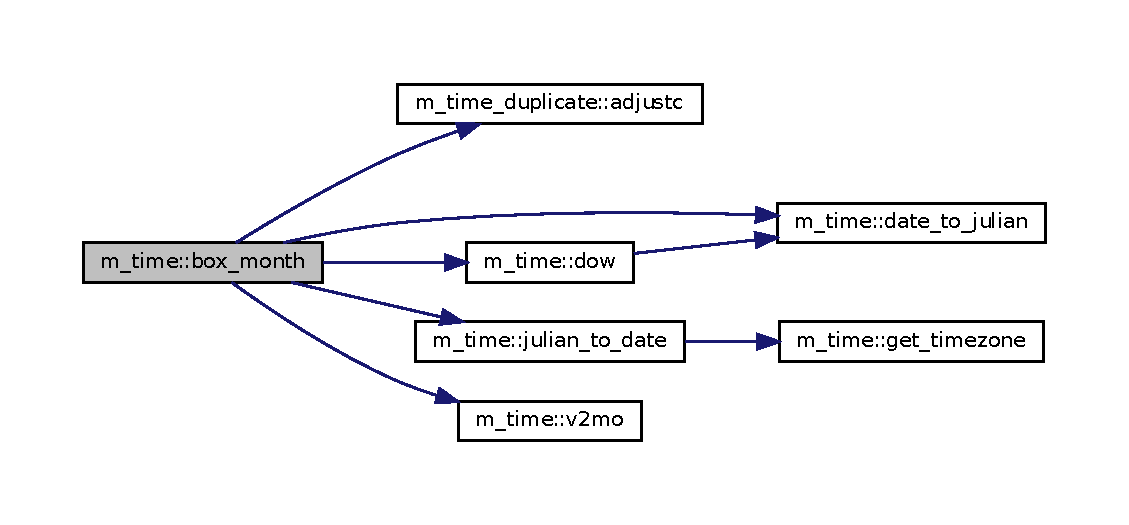
\includegraphics[width=350pt]{namespacem__time_a0fe7540912df30d3578f3c469413aea8_cgraph}
\end{center}
\end{figure}
\mbox{\Hypertarget{namespacem__time_af558bfc1fd5b13a6b879b3969866956f}\label{namespacem__time_af558bfc1fd5b13a6b879b3969866956f}} 
\index{m\_time@{m\_time}!call\_sleep@{call\_sleep}}
\index{call\_sleep@{call\_sleep}!m\_time@{m\_time}}
\doxysubsubsection{\texorpdfstring{call\_sleep()}{call\_sleep()}}
{\footnotesize\ttfamily subroutine, private m\+\_\+time\+::call\+\_\+sleep (\begin{DoxyParamCaption}\item[{integer(kind=c\+\_\+int), intent(in)}]{wait\+\_\+seconds }\end{DoxyParamCaption})\hspace{0.3cm}{\ttfamily [private]}}

Here is the caller graph for this function\+:\nopagebreak
\begin{figure}[H]
\begin{center}
\leavevmode
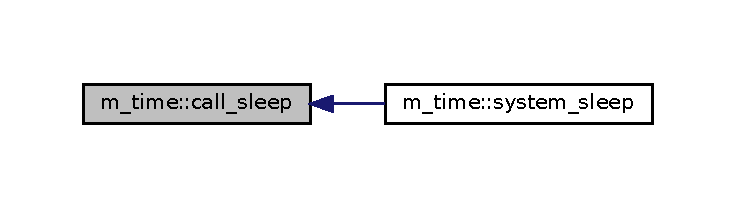
\includegraphics[width=350pt]{namespacem__time_af558bfc1fd5b13a6b879b3969866956f_icgraph}
\end{center}
\end{figure}
\mbox{\Hypertarget{namespacem__time_ae63783f7479d2f5093c8031d38ce4304}\label{namespacem__time_ae63783f7479d2f5093c8031d38ce4304}} 
\index{m\_time@{m\_time}!call\_usleep@{call\_usleep}}
\index{call\_usleep@{call\_usleep}!m\_time@{m\_time}}
\doxysubsubsection{\texorpdfstring{call\_usleep()}{call\_usleep()}}
{\footnotesize\ttfamily subroutine, private m\+\_\+time\+::call\+\_\+usleep (\begin{DoxyParamCaption}\item[{integer(kind=c\+\_\+int), intent(in)}]{wait\+\_\+seconds }\end{DoxyParamCaption})\hspace{0.3cm}{\ttfamily [private]}}

Here is the caller graph for this function\+:\nopagebreak
\begin{figure}[H]
\begin{center}
\leavevmode
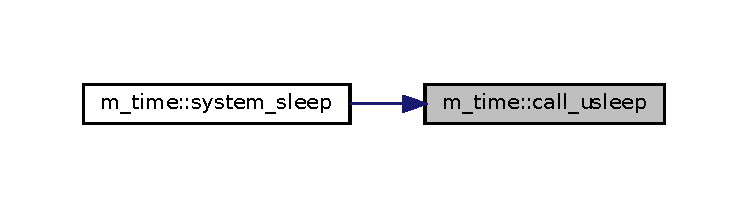
\includegraphics[width=350pt]{namespacem__time_ae63783f7479d2f5093c8031d38ce4304_icgraph}
\end{center}
\end{figure}
\mbox{\Hypertarget{namespacem__time_a3fccc53c2650104eff084c7998d18f54}\label{namespacem__time_a3fccc53c2650104eff084c7998d18f54}} 
\index{m\_time@{m\_time}!d2j@{d2j}}
\index{d2j@{d2j}!m\_time@{m\_time}}
\doxysubsubsection{\texorpdfstring{d2j()}{d2j()}}
{\footnotesize\ttfamily real(kind=\mbox{\hyperlink{namespacem__time_ac10ea9e8d59ec74eaa7d89f2517d7422}{realtime}}) function, public m\+\_\+time\+::d2j (\begin{DoxyParamCaption}\item[{integer, dimension(8), intent(in), optional}]{dat }\end{DoxyParamCaption})}

\hypertarget{namespacem__time_autotoc_md160}{}\doxysubsubsection{N\+A\+ME}\label{namespacem__time_autotoc_md160}
d2j(3f) -\/ \mbox{[}M\+\_\+time\+:J\+U\+L\+I\+AN\mbox{]} given D\+AT date-\/time array returns Julian Date (L\+I\+C\+E\+N\+SE\+:PD)\hypertarget{namespacem__time_autotoc_md161}{}\doxysubsubsection{S\+Y\+N\+O\+P\+S\+IS}\label{namespacem__time_autotoc_md161}
\begin{DoxyVerb}function d2j(dat) result (julian)

 integer,intent(in)  :: dat(8)
 real(kind=realtime) :: julian
\end{DoxyVerb}
\hypertarget{namespacem__time_autotoc_md162}{}\doxysubsubsection{D\+E\+S\+C\+R\+I\+P\+T\+I\+ON}\label{namespacem__time_autotoc_md162}
Given D\+AT date-\/time array returns Julian Date\hypertarget{namespacem__time_autotoc_md163}{}\doxysubsubsection{O\+P\+T\+I\+O\+NS}\label{namespacem__time_autotoc_md163}
dat Integer array holding a \char`\"{}\+D\+A\+T\char`\"{} array, similar in structure to the array returned by the intrinsic D\+A\+T\+E\+\_\+\+A\+N\+D\+\_\+\+T\+I\+M\+E(3f)\+:

dat=\mbox{[} year,month,day,timezone,hour,\& \& minutes,seconds,milliseconds\mbox{]}

If not present, use current time. \hypertarget{namespacem__time_autotoc_md164}{}\doxysubsubsection{R\+E\+T\+U\+R\+NS}\label{namespacem__time_autotoc_md164}
julian The Julian Date.\hypertarget{namespacem__time_autotoc_md165}{}\doxysubsubsection{E\+X\+A\+M\+P\+LE}\label{namespacem__time_autotoc_md165}
\begin{DoxyVerb}Sample program:

 program demo_d2j
 use M_time, only : d2j
 implicit none
 integer :: dat(8)
    call date_and_time(values=dat)
    write(*,'(" Today is:",*(i0:,":"))')dat
    write(*,*)'Julian Date is ',d2j(dat)
 end program demo_d2j

results:

 Today is:2016:7:19:-240:2:11:50:885
 Julian Date is    2457588.7582278359
\end{DoxyVerb}
\hypertarget{namespacem__time_autotoc_md166}{}\doxysubsubsection{A\+U\+T\+H\+OR}\label{namespacem__time_autotoc_md166}
John S. Urban, 2015 \hypertarget{namespacem__time_autotoc_md167}{}\doxysubsubsection{L\+I\+C\+E\+N\+SE}\label{namespacem__time_autotoc_md167}
Public Domain 

References date\+\_\+to\+\_\+julian().

Here is the call graph for this function\+:\nopagebreak
\begin{figure}[H]
\begin{center}
\leavevmode
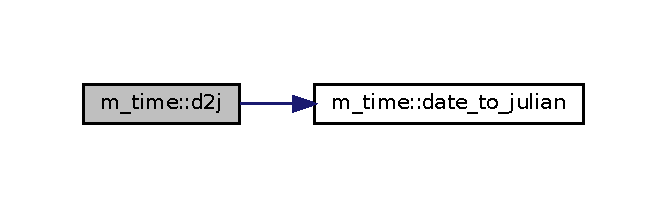
\includegraphics[width=320pt]{namespacem__time_a3fccc53c2650104eff084c7998d18f54_cgraph}
\end{center}
\end{figure}
Here is the caller graph for this function\+:\nopagebreak
\begin{figure}[H]
\begin{center}
\leavevmode
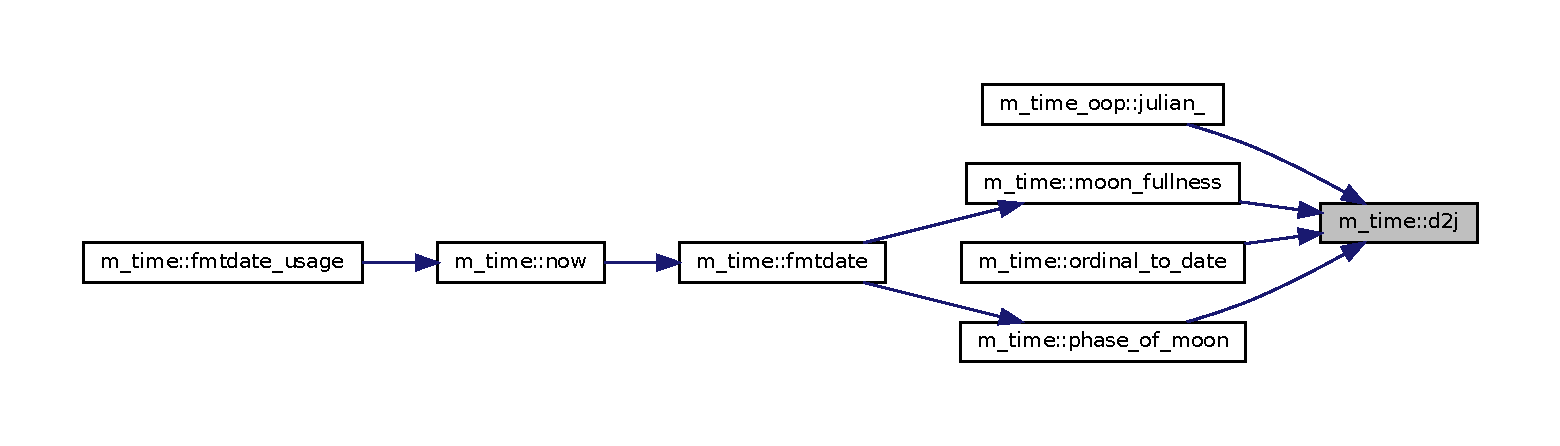
\includegraphics[width=350pt]{namespacem__time_a3fccc53c2650104eff084c7998d18f54_icgraph}
\end{center}
\end{figure}
\mbox{\Hypertarget{namespacem__time_a727dd77bbd4a5d0e3947c5d303845947}\label{namespacem__time_a727dd77bbd4a5d0e3947c5d303845947}} 
\index{m\_time@{m\_time}!d2o@{d2o}}
\index{d2o@{d2o}!m\_time@{m\_time}}
\doxysubsubsection{\texorpdfstring{d2o()}{d2o()}}
{\footnotesize\ttfamily integer function, public m\+\_\+time\+::d2o (\begin{DoxyParamCaption}\item[{integer, dimension(8), intent(in), optional}]{dat }\end{DoxyParamCaption})}

\hypertarget{namespacem__time_autotoc_md34}{}\doxysubsubsection{N\+A\+ME}\label{namespacem__time_autotoc_md34}
d2o(3f) -\/ \mbox{[}M\+\_\+time\+:O\+R\+D\+I\+N\+A\+L\+\_\+\+D\+AY\mbox{]} converts D\+AT date-\/time array to Ordinal day (L\+I\+C\+E\+N\+SE\+:PD)\hypertarget{namespacem__time_autotoc_md35}{}\doxysubsubsection{S\+Y\+N\+O\+P\+S\+IS}\label{namespacem__time_autotoc_md35}
\begin{DoxyVerb}function d2o(dat) result (ordinal)

 integer,intent(in),optional :: dat(8)
 integer                     :: ordinal
\end{DoxyVerb}
\hypertarget{namespacem__time_autotoc_md36}{}\doxysubsubsection{D\+E\+S\+C\+R\+I\+P\+T\+I\+ON}\label{namespacem__time_autotoc_md36}
Given a date in the form of a \char`\"{}\+D\+A\+T\char`\"{} array return the Ordinal Day, (ie. \char`\"{}the day of the year\char`\"{}).\hypertarget{namespacem__time_autotoc_md37}{}\doxysubsubsection{O\+P\+T\+I\+O\+NS}\label{namespacem__time_autotoc_md37}
dat Integer array holding a \char`\"{}\+D\+A\+T\char`\"{} array, similar in structure to the array returned by the intrinsic D\+A\+T\+E\+\_\+\+A\+N\+D\+\_\+\+T\+I\+M\+E(3f)\+: \begin{DoxyVerb}dat=[ year,month,day,timezone,hour,&
 & minutes,seconds,milliseconds]
\end{DoxyVerb}
 \hypertarget{namespacem__time_autotoc_md38}{}\doxysubsubsection{R\+E\+T\+U\+R\+NS}\label{namespacem__time_autotoc_md38}
ordinal The day of the year calculated for the given input date, where Jan 1st=1.\hypertarget{namespacem__time_autotoc_md39}{}\doxysubsubsection{E\+X\+A\+M\+P\+LE}\label{namespacem__time_autotoc_md39}
\begin{DoxyVerb}Sample program:

 program demo_d2o
 use M_time, only : d2o
 implicit none
 integer :: dat(8)
    call date_and_time(values=dat)
    write(*,'(" Today is:",*(i0:,":"))')dat
    write(*,*)'Day of year is:',d2o(dat)

    ! year,month,day,timezone,hour,minute,seconds,milliseconds
    dat=[2020,12,31,-240,12,0,0,0]
    write(*,*)dat(1),' Days in year is:',d2o(dat)

    dat=[2021,12,31,-240,12,0,0,0]
    write(*,*)dat(1),' Days in year is:',d2o(dat)

    dat=[2022,12,31,-240,12,0,0,0]
    write(*,*)dat(1),' Days in year is:',d2o(dat)

    dat=[2023,12,31,-240,12,0,0,0]
    write(*,*)dat(1),' Days in year is:',d2o(dat)

    dat=[2024,12,31,-240,12,0,0,0]
    write(*,*)dat(1),' Days in year is:',d2o(dat)

 end program demo_d2o

results:

 Today is:2016:7:19:-240:20:1:19:829
 Day of year is:         201
        2020  Days in year is:         366
        2021  Days in year is:         365
        2022  Days in year is:         365
        2023  Days in year is:         365
        2024  Days in year is:         366
\end{DoxyVerb}
\hypertarget{namespacem__time_autotoc_md40}{}\doxysubsubsection{A\+U\+T\+H\+OR}\label{namespacem__time_autotoc_md40}
John S. Urban, 2015 \hypertarget{namespacem__time_autotoc_md41}{}\doxysubsubsection{L\+I\+C\+E\+N\+SE}\label{namespacem__time_autotoc_md41}
Public Domain 

References date\+\_\+to\+\_\+unix(), secday, and m\+\_\+time\+\_\+duplicate\+::stderr().

Here is the call graph for this function\+:\nopagebreak
\begin{figure}[H]
\begin{center}
\leavevmode
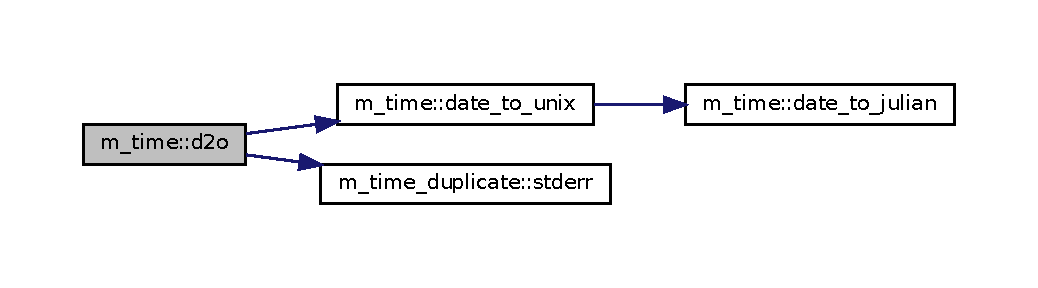
\includegraphics[width=350pt]{namespacem__time_a727dd77bbd4a5d0e3947c5d303845947_cgraph}
\end{center}
\end{figure}
Here is the caller graph for this function\+:\nopagebreak
\begin{figure}[H]
\begin{center}
\leavevmode
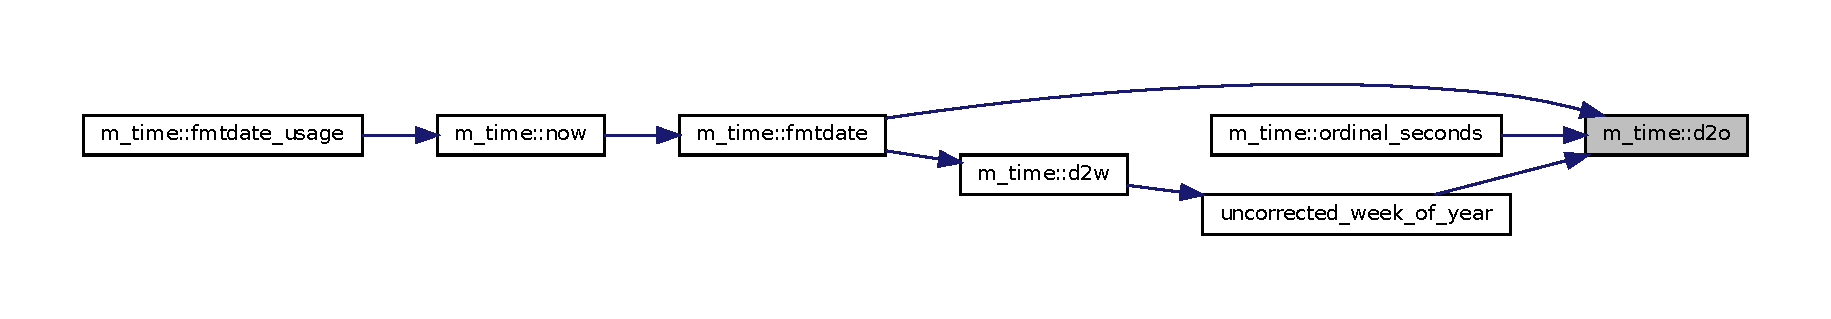
\includegraphics[width=350pt]{namespacem__time_a727dd77bbd4a5d0e3947c5d303845947_icgraph}
\end{center}
\end{figure}
\mbox{\Hypertarget{namespacem__time_a1506e2889a156387df4481ed0534be81}\label{namespacem__time_a1506e2889a156387df4481ed0534be81}} 
\index{m\_time@{m\_time}!d2u@{d2u}}
\index{d2u@{d2u}!m\_time@{m\_time}}
\doxysubsubsection{\texorpdfstring{d2u()}{d2u()}}
{\footnotesize\ttfamily real(kind=\mbox{\hyperlink{namespacem__time_ac10ea9e8d59ec74eaa7d89f2517d7422}{realtime}}) function, public m\+\_\+time\+::d2u (\begin{DoxyParamCaption}\item[{integer, dimension(8), intent(in), optional}]{dat }\end{DoxyParamCaption})}

\hypertarget{namespacem__time_autotoc_md176}{}\doxysubsubsection{N\+A\+ME}\label{namespacem__time_autotoc_md176}
d2u(3f) -\/ \mbox{[}M\+\_\+time\+:U\+N\+I\+X\+\_\+\+E\+P\+O\+CH\mbox{]} given D\+AT date-\/time array returns Unix Epoch Time (U\+ET starts at 0000 on 1 Jan. 1970, U\+TC) (L\+I\+C\+E\+N\+SE\+:PD)\hypertarget{namespacem__time_autotoc_md177}{}\doxysubsubsection{S\+Y\+N\+O\+P\+S\+IS}\label{namespacem__time_autotoc_md177}
\begin{DoxyVerb}function d2u(dat) result (unixtime)

   integer,intent(in),optional :: dat(8)
   real(kind=realtime)         :: unixtime
\end{DoxyVerb}
\hypertarget{namespacem__time_autotoc_md178}{}\doxysubsubsection{D\+E\+S\+C\+R\+I\+P\+T\+I\+ON}\label{namespacem__time_autotoc_md178}
Converts a D\+AT date-\/time array to a Unix Epoch Time value. Typically mathematical operations such as sums, sorting and comparison are performed with simple U\+ET numeric values, and then they are converted back.\hypertarget{namespacem__time_autotoc_md179}{}\doxysubsubsection{O\+P\+T\+I\+O\+NS}\label{namespacem__time_autotoc_md179}
dat Integer array holding a \char`\"{}\+D\+A\+T\char`\"{} array, similar in structure to the array returned by the intrinsic D\+A\+T\+E\+\_\+\+A\+N\+D\+\_\+\+T\+I\+M\+E(3f)\+: \begin{DoxyVerb}   dat=[ year,month,day,timezone,hour,&
    & minutes,seconds,milliseconds]
\end{DoxyVerb}


If not present the current time is used\hypertarget{namespacem__time_autotoc_md180}{}\doxysubsubsection{R\+E\+T\+U\+R\+NS}\label{namespacem__time_autotoc_md180}
unixtime The \char`\"{}\+Unix Epoch\char`\"{} time, or the number of seconds since 00\+:00\+:00 on January 1st, 1970, U\+TC.\hypertarget{namespacem__time_autotoc_md181}{}\doxysubsubsection{E\+X\+A\+M\+P\+LE}\label{namespacem__time_autotoc_md181}
\begin{DoxyVerb}Sample program:

 program demo_d2u
 use M_time, only : d2u
 implicit none
 integer           :: dat(8)
    call date_and_time(values=dat)
    write(*,'(" Today is:",*(i0:,":"))')dat
    write(*,*)'Unix Epoch time is ',d2u(dat)
 end program demo_d2u

results:

 Today is:2016:7:19:-240:2:0:48:561
 Unix Epoch time is    1468908048.5610321
\end{DoxyVerb}
 \hypertarget{namespacem__time_autotoc_md182}{}\doxysubsubsection{A\+U\+T\+H\+OR}\label{namespacem__time_autotoc_md182}
John S. Urban, 2015 \hypertarget{namespacem__time_autotoc_md183}{}\doxysubsubsection{L\+I\+C\+E\+N\+SE}\label{namespacem__time_autotoc_md183}
Public Domain 

References date\+\_\+to\+\_\+unix().

Here is the call graph for this function\+:\nopagebreak
\begin{figure}[H]
\begin{center}
\leavevmode
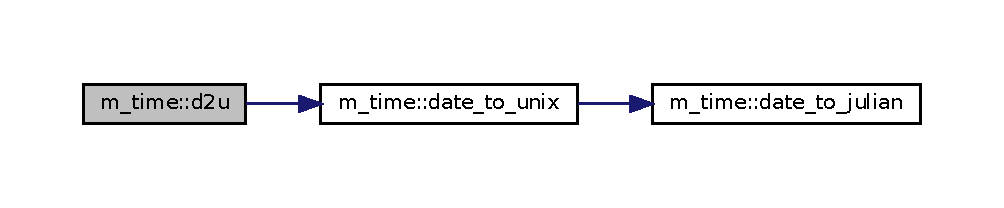
\includegraphics[width=350pt]{namespacem__time_a1506e2889a156387df4481ed0534be81_cgraph}
\end{center}
\end{figure}
Here is the caller graph for this function\+:\nopagebreak
\begin{figure}[H]
\begin{center}
\leavevmode
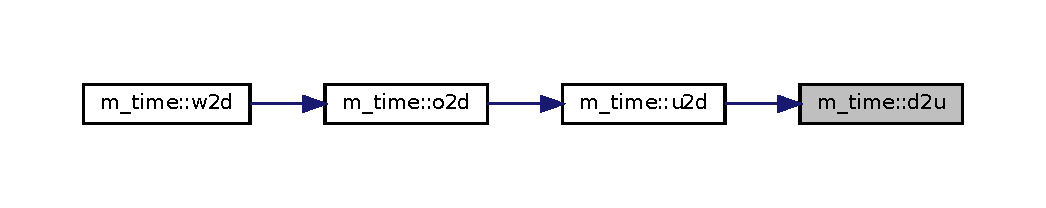
\includegraphics[width=350pt]{namespacem__time_a1506e2889a156387df4481ed0534be81_icgraph}
\end{center}
\end{figure}
\mbox{\Hypertarget{namespacem__time_ad4ff99ad6f6d5282c4b65ad636a2a627}\label{namespacem__time_ad4ff99ad6f6d5282c4b65ad636a2a627}} 
\index{m\_time@{m\_time}!d2w@{d2w}}
\index{d2w@{d2w}!m\_time@{m\_time}}
\doxysubsubsection{\texorpdfstring{d2w()}{d2w()}}
{\footnotesize\ttfamily subroutine, public m\+\_\+time\+::d2w (\begin{DoxyParamCaption}\item[{integer, dimension(8), intent(in)}]{dat,  }\item[{integer, intent(out)}]{iso\+\_\+year,  }\item[{integer, intent(out)}]{iso\+\_\+week,  }\item[{integer, intent(out)}]{iso\+\_\+weekday,  }\item[{character(len=10), intent(out)}]{iso\+\_\+name }\end{DoxyParamCaption})}

\hypertarget{namespacem__time_autotoc_md123}{}\doxysubsubsection{N\+A\+ME}\label{namespacem__time_autotoc_md123}
d2w(3f) -\/ \mbox{[}M\+\_\+time\+:W\+E\+E\+K\+\_\+\+O\+F\+\_\+\+Y\+E\+AR\mbox{]} calculate iso-\/8601 Week-\/numbering year date yyyy-\/\+Www-\/d given D\+AT date-\/time array (L\+I\+C\+E\+N\+SE\+:PD)\hypertarget{namespacem__time_autotoc_md124}{}\doxysubsubsection{S\+Y\+N\+O\+P\+S\+IS}\label{namespacem__time_autotoc_md124}
\begin{DoxyVerb}subroutine d2w(dat,iso_year,iso_week,iso_weekday,iso_name)

 integer,intent(in)              :: dat(8)     ! input date array
 integer,intent(out)             :: iso_year, iso_week, iso_weekday
 character(len=10),intent(out)   :: iso_name
\end{DoxyVerb}
\hypertarget{namespacem__time_autotoc_md125}{}\doxysubsubsection{D\+E\+S\+C\+R\+I\+P\+T\+I\+ON}\label{namespacem__time_autotoc_md125}
Given a \char`\"{}\+D\+A\+T\char`\"{} array defining a date and time, return the I\+S\+O-\/8601 Week in two formats -- as three integer values defining the I\+SO year, week of year and weekday; and as a string of the form \char`\"{}yyyy-\/\+Www-\/d\char`\"{}.\hypertarget{namespacem__time_autotoc_md126}{}\doxysubsubsection{O\+P\+T\+I\+O\+NS}\label{namespacem__time_autotoc_md126}
dat \char`\"{}\+D\+A\+T\char`\"{} array (an integer array of the same format as the array returned by the intrinsic D\+A\+T\+E\+\_\+\+A\+N\+D\+\_\+\+T\+I\+M\+E(3f)) describing the date, which is the basic time description used by the other M\+\_\+time(3fm) module procedures. \hypertarget{namespacem__time_autotoc_md127}{}\doxysubsubsection{R\+E\+T\+U\+R\+NS}\label{namespacem__time_autotoc_md127}
iso\+\_\+year I\+S\+O-\/8601 year number for the given date iso\+\_\+week I\+S\+O-\/8601 week number for the given date iso\+\_\+weekday I\+S\+O-\/8601 weekday number for the given date iso\+\_\+name I\+S\+O-\/8601 Week string for the data in the form \char`\"{}yyyy-\/\+Www-\/d\char`\"{}.\hypertarget{namespacem__time_autotoc_md128}{}\doxysubsubsection{E\+X\+A\+M\+P\+LE}\label{namespacem__time_autotoc_md128}
\begin{DoxyVerb}Sample program:

 program demo_d2w
 use M_time, only : d2w
 implicit none
 integer           :: dat(8)     ! input date array
 integer           :: iso_year, iso_week, iso_weekday
 character(len=10) :: iso_name
    call date_and_time(values=dat)
    call d2w(dat,iso_year,iso_week,iso_weekday,iso_name)
    write(*,'("ISO-8601 Week:   ",a)')iso_name
    write(*,'(a,i0)')'ISO-8601 year    ',iso_year
    write(*,'(a,i0)')'ISO-8601 week    ',iso_week
    write(*,'(a,i0)')'ISO-8601 weekday ',iso_weekday
 end program demo_d2w

results:

 ISO-8601 Week:   2016-W29-1
 ISO-8601 year    2016
 ISO-8601 week    29
 ISO-8601 weekday 1
\end{DoxyVerb}
\hypertarget{namespacem__time_autotoc_md129}{}\doxysubsubsection{D\+E\+F\+I\+N\+I\+T\+I\+ON}\label{namespacem__time_autotoc_md129}
The I\+S\+O-\/8601 date and time standard was issued by the International Organization for Standardization (I\+SO). It is used (mainly) in government and business for fiscal years, as well as in timekeeping. The system specifies a week year atop the Gregorian calendar by defining a notation for ordinal weeks of the year.

An I\+SO week-\/numbering year (also called I\+SO year informally) has 52 or 53 full weeks. That is 364 or 371 days instead of the usual 365 or 366 days. The extra week is referred to here as a leap week, although I\+S\+O-\/8601 does not use this term. Weeks start with Monday. The first week of a year is the week that contains the first Thursday of the year (and, hence, always contains 4 January). I\+SO week year numbering therefore slightly deviates from the Gregorian for some days close to January 1st.\hypertarget{namespacem__time_autotoc_md130}{}\doxysubsubsection{C\+A\+L\+C\+U\+L\+A\+T\+I\+ON}\label{namespacem__time_autotoc_md130}
The I\+S\+O-\/8601 week number of any date can be calculated, given its ordinal date (i.\+e. position within the year) and its day of the week.\hypertarget{namespacem__time_autotoc_md131}{}\doxysubsubsection{M\+E\+T\+H\+OD}\label{namespacem__time_autotoc_md131}
Using I\+SO weekday numbers (running from 1 for Monday to 7 for Sunday), subtract the weekday from the ordinal date, then add 10. Divide the result by 7. Ignore the remainder; the quotient equals the week number. If the week number thus obtained equals 0, it means that the given date belongs to the preceding (week-\/based) year. If a week number of 53 is obtained, one must check that the date is not actually in week 1 of the following year.

These two statements are assumed true when correcting the dates around January 1st\+:

o The number of weeks in a given year is equal to the corresponding week number of 28 December. o January 4th is always in the first week.\hypertarget{namespacem__time_autotoc_md132}{}\doxysubsubsection{I\+S\+O\+\_\+\+N\+A\+ME}\label{namespacem__time_autotoc_md132}
Week date representations are in the format Y\+Y\+Y\+Y\+Www-\/D.

o \mbox{[}Y\+Y\+YY\mbox{]} indicates the I\+SO week-\/numbering year which is slightly different from the traditional Gregorian calendar year. o \mbox{[}Www\mbox{]} is the week number prefixed by the letter W, from W01 through W53. o \mbox{[}D\mbox{]} is the weekday number, from 1 through 7, beginning with Monday and ending with Sunday.

For example, the Gregorian date 31 December 2006 corresponds to the Sunday of the 52nd week of 2006, and is written

2006-\/W52-\/7 (extended form) or 2006W527 (compact form).\hypertarget{namespacem__time_autotoc_md133}{}\doxysubsubsection{R\+E\+F\+E\+R\+E\+N\+CE}\label{namespacem__time_autotoc_md133}
From Wikipedia, the free encyclopedia 2015-\/12-\/19\hypertarget{namespacem__time_autotoc_md134}{}\doxysubsubsection{A\+U\+T\+H\+OR}\label{namespacem__time_autotoc_md134}
John S. Urban, 2015-\/12-\/19 \hypertarget{namespacem__time_autotoc_md135}{}\doxysubsubsection{L\+I\+C\+E\+N\+SE}\label{namespacem__time_autotoc_md135}
Public Domain 

References uncorrected\+\_\+week\+\_\+of\+\_\+year().

Here is the call graph for this function\+:\nopagebreak
\begin{figure}[H]
\begin{center}
\leavevmode
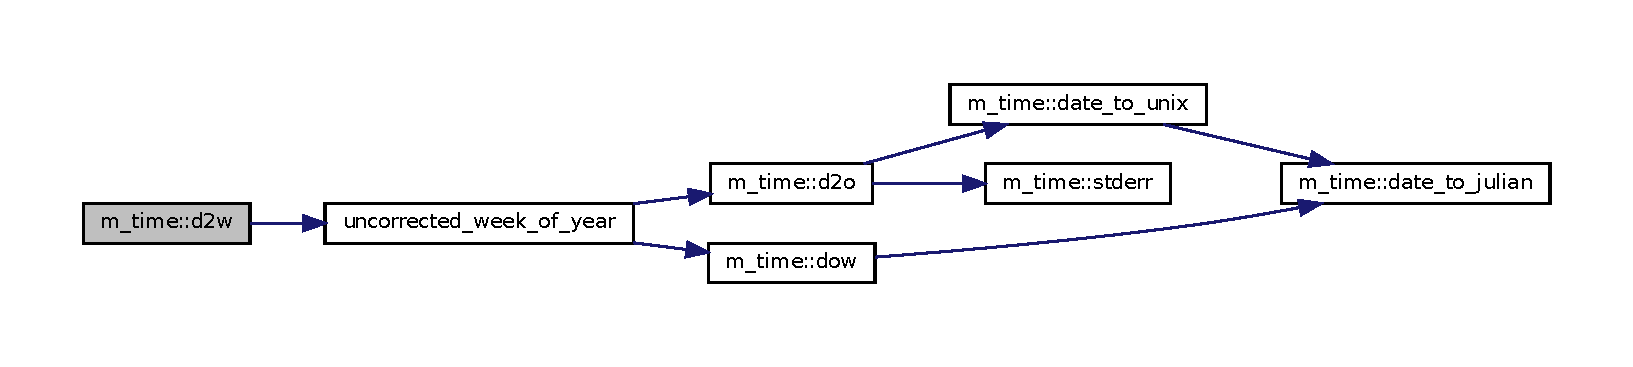
\includegraphics[width=350pt]{namespacem__time_ad4ff99ad6f6d5282c4b65ad636a2a627_cgraph}
\end{center}
\end{figure}
Here is the caller graph for this function\+:\nopagebreak
\begin{figure}[H]
\begin{center}
\leavevmode
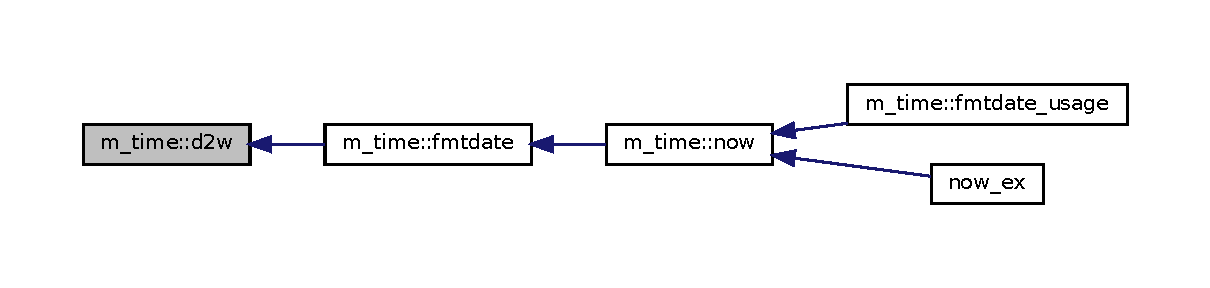
\includegraphics[width=350pt]{namespacem__time_ad4ff99ad6f6d5282c4b65ad636a2a627_icgraph}
\end{center}
\end{figure}
\mbox{\Hypertarget{namespacem__time_acfdc970b4154b0c15bd33727636e3992}\label{namespacem__time_acfdc970b4154b0c15bd33727636e3992}} 
\index{m\_time@{m\_time}!date\_to\_julian@{date\_to\_julian}}
\index{date\_to\_julian@{date\_to\_julian}!m\_time@{m\_time}}
\doxysubsubsection{\texorpdfstring{date\_to\_julian()}{date\_to\_julian()}}
{\footnotesize\ttfamily subroutine, public m\+\_\+time\+::date\+\_\+to\+\_\+julian (\begin{DoxyParamCaption}\item[{integer, dimension(8), intent(in)}]{dat,  }\item[{real(kind=\mbox{\hyperlink{namespacem__time_ac10ea9e8d59ec74eaa7d89f2517d7422}{realtime}}), intent(out)}]{julian,  }\item[{integer, intent(out)}]{ierr }\end{DoxyParamCaption})}

\hypertarget{namespacem__time_autotoc_md0}{}\doxysubsubsection{N\+A\+ME}\label{namespacem__time_autotoc_md0}
date\+\_\+to\+\_\+julian(3f) -\/ \mbox{[}M\+\_\+time\+:J\+U\+L\+I\+AN\mbox{]} converts D\+AT date-\/time array to Julian Date (L\+I\+C\+E\+N\+SE\+:PD)\hypertarget{namespacem__time_autotoc_md1}{}\doxysubsubsection{S\+Y\+N\+O\+P\+S\+IS}\label{namespacem__time_autotoc_md1}
\begin{DoxyVerb}subroutine date_to_julian(dat,juliandate,ierr)

 integer,intent(in)               :: dat(8)
 real(kind=realtime),intent(out)  :: juliandate
 integer,intent(out)              :: ierr
\end{DoxyVerb}
\hypertarget{namespacem__time_autotoc_md2}{}\doxysubsubsection{D\+E\+S\+C\+R\+I\+P\+T\+I\+ON}\label{namespacem__time_autotoc_md2}
Converts a D\+AT date-\/time array to a Unix Epoch Time (U\+ET) value. U\+ET is the number of seconds since 00\+:00 on January 1st, 1970, U\+TC.\hypertarget{namespacem__time_autotoc_md3}{}\doxysubsubsection{O\+P\+T\+I\+O\+NS}\label{namespacem__time_autotoc_md3}
dat Integer array holding a \char`\"{}\+D\+A\+T\char`\"{} array, similar in structure to the array returned by the intrinsic D\+A\+T\+E\+\_\+\+A\+N\+D\+\_\+\+T\+I\+M\+E(3f)\+:

dat=\mbox{[} year,month,day,timezone,hour,\& \& minutes,seconds,milliseconds\mbox{]}\hypertarget{namespacem__time_autotoc_md4}{}\doxysubsubsection{R\+E\+T\+U\+R\+NS}\label{namespacem__time_autotoc_md4}
juliandate A Julian Ephemeris Date (J\+ED) is the number of days since noon (not midnight) on January 1st, 4713 BC. ierr Error code. If 0 no error occurred.\hypertarget{namespacem__time_autotoc_md5}{}\doxysubsubsection{E\+X\+A\+M\+P\+LE}\label{namespacem__time_autotoc_md5}
\begin{DoxyVerb}Sample Program:

 program demo_date_to_julian
 use M_time, only : date_to_julian,realtime
 implicit none
 integer             :: dat(8)
 real(kind=realtime) :: juliandate
 integer             :: ierr
    ! generate DAT array
    call date_and_time(values=dat)
    ! show DAT array
    write(*,'(" Today is:",*(i0:,":"))')dat
    ! convert DAT to Julian Date
    call date_to_julian(dat,juliandate,ierr)
    write(*,*)'Julian Date is ',juliandate
    write(*,*)'ierr is ',ierr
 end program demo_date_to_julian

results:

 Today is:2016:7:19:-240:11:3:13:821
 Julian Date is    2457589.1272432986
 ierr is            0
\end{DoxyVerb}
\hypertarget{namespacem__time_autotoc_md6}{}\doxysubsubsection{A\+U\+T\+H\+OR}\label{namespacem__time_autotoc_md6}
John S. Urban, 2015 \hypertarget{namespacem__time_autotoc_md7}{}\doxysubsubsection{L\+I\+C\+E\+N\+SE}\label{namespacem__time_autotoc_md7}
Public Domain
\begin{DoxyParams}[1]{Parameters}
\mbox{\texttt{ in}}  & {\em dat} & A\+U\+T\+H\+OR\+: John S. Urban \\
\hline
\end{DoxyParams}
\hypertarget{namespacem__time_autotoc_md9}{}\doxysubsubsection{V\+E\+R\+S\+I\+O\+N\+:   2.\+0 2022-\/01-\/16}\label{namespacem__time_autotoc_md9}
R\+E\+F\+E\+R\+E\+N\+CE\+: From Wikipedia, the free encyclopedia 2015-\/12-\/19 Here is the caller graph for this function\+:\nopagebreak
\begin{figure}[H]
\begin{center}
\leavevmode
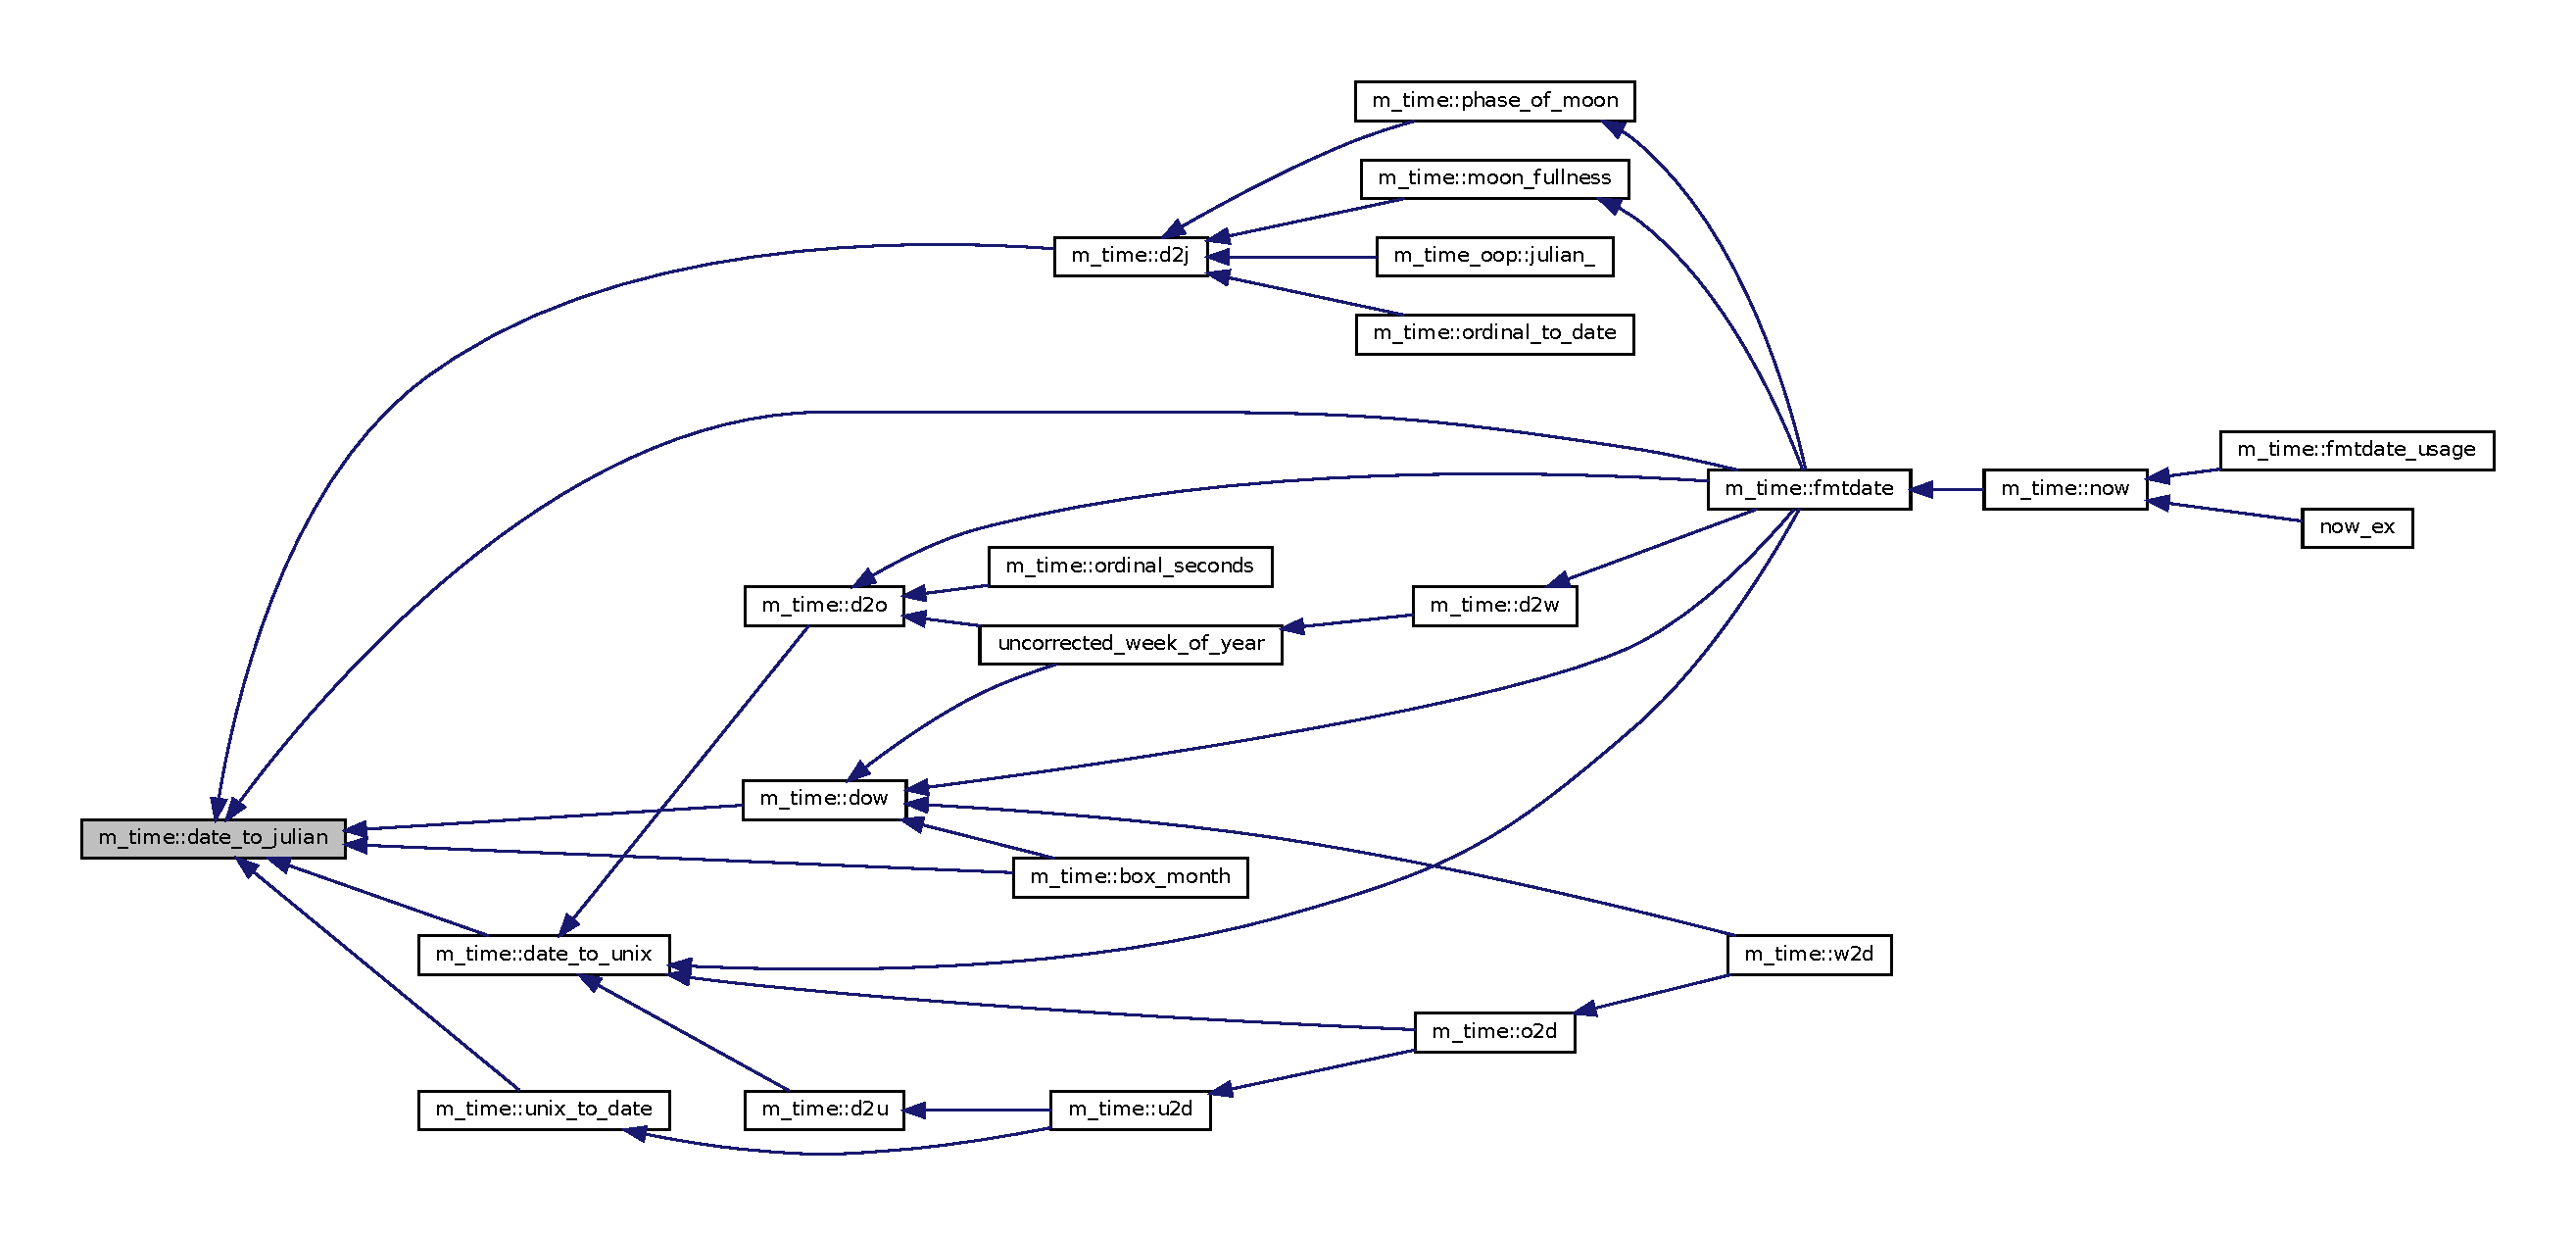
\includegraphics[width=350pt]{namespacem__time_acfdc970b4154b0c15bd33727636e3992_icgraph}
\end{center}
\end{figure}
\mbox{\Hypertarget{namespacem__time_aed245c691853279ebf0ce899dec9caa9}\label{namespacem__time_aed245c691853279ebf0ce899dec9caa9}} 
\index{m\_time@{m\_time}!date\_to\_unix@{date\_to\_unix}}
\index{date\_to\_unix@{date\_to\_unix}!m\_time@{m\_time}}
\doxysubsubsection{\texorpdfstring{date\_to\_unix()}{date\_to\_unix()}}
{\footnotesize\ttfamily subroutine, public m\+\_\+time\+::date\+\_\+to\+\_\+unix (\begin{DoxyParamCaption}\item[{integer, dimension(8), intent(in)}]{dat,  }\item[{real(kind=\mbox{\hyperlink{namespacem__time_ac10ea9e8d59ec74eaa7d89f2517d7422}{realtime}}), intent(out)}]{unixtime,  }\item[{integer, intent(out)}]{ierr }\end{DoxyParamCaption})}

\hypertarget{namespacem__time_autotoc_md18}{}\doxysubsubsection{N\+A\+ME}\label{namespacem__time_autotoc_md18}
date\+\_\+to\+\_\+unix(3f) -\/ \mbox{[}M\+\_\+time\+:U\+N\+I\+X\+\_\+\+E\+P\+O\+CH\mbox{]} converts D\+AT date-\/time array to Unix Epoch Time (L\+I\+C\+E\+N\+SE\+:PD)\hypertarget{namespacem__time_autotoc_md19}{}\doxysubsubsection{S\+Y\+N\+O\+P\+S\+IS}\label{namespacem__time_autotoc_md19}
\begin{DoxyVerb}subroutine date_to_unix(dat,unixtime,ierr)

 integer,intent(in)               :: dat(8)
 real(kind=realtime),intent(out)  :: unixtime
 integer,intent(out)              :: ierr
\end{DoxyVerb}
\hypertarget{namespacem__time_autotoc_md20}{}\doxysubsubsection{D\+E\+S\+C\+R\+I\+P\+T\+I\+ON}\label{namespacem__time_autotoc_md20}
Converts a D\+AT date-\/time array to a U\+ET (Unix Epoch Time).\hypertarget{namespacem__time_autotoc_md21}{}\doxysubsubsection{O\+P\+T\+I\+O\+NS}\label{namespacem__time_autotoc_md21}
dat Integer array holding a \char`\"{}\+D\+A\+T\char`\"{} array, similar in structure to the array returned by the intrinsic D\+A\+T\+E\+\_\+\+A\+N\+D\+\_\+\+T\+I\+M\+E(3f)\+: \begin{DoxyVerb}dat=[ year,month,day,timezone,hour,&
 & minutes,seconds,milliseconds]
\end{DoxyVerb}
 \hypertarget{namespacem__time_autotoc_md22}{}\doxysubsubsection{R\+E\+T\+U\+R\+NS}\label{namespacem__time_autotoc_md22}
unixtime The \char`\"{}\+Unix Epoch\char`\"{} time, or the number of seconds since 00\+:00\+:00 on January 1st, 1970, U\+TC. ierr Error code. If 0 no error occurred.\hypertarget{namespacem__time_autotoc_md23}{}\doxysubsubsection{E\+X\+A\+M\+P\+LE}\label{namespacem__time_autotoc_md23}
\begin{DoxyVerb} Sample program:

  program demo_date_to_unix
  use M_time, only : date_to_unix, realtime
  implicit none
  integer             :: dat(8)
  real(kind=realtime) :: unixtime
  integer             :: ierr
     call date_and_time(values=dat)
     write(*,'(" Today is:",*(i0:,":"))')dat
     call date_to_unix(dat,unixtime,ierr)
     write(*,*)'Unix Epoch time is ',unixtime
     write(*,*)'ierr is ',ierr
  end program demo_date_to_unix

 results:

  Today is:2016:7:18:-240:23:44:20:434
  Unix Epoch time is    1468899860.4340105
  ierr is            0
\end{DoxyVerb}
 \hypertarget{namespacem__time_autotoc_md24}{}\doxysubsubsection{A\+U\+T\+H\+OR}\label{namespacem__time_autotoc_md24}
John S. Urban, 2015 \hypertarget{namespacem__time_autotoc_md25}{}\doxysubsubsection{L\+I\+C\+E\+N\+SE}\label{namespacem__time_autotoc_md25}
Public Domain 

References date\+\_\+to\+\_\+julian(), and secday.

Here is the call graph for this function\+:\nopagebreak
\begin{figure}[H]
\begin{center}
\leavevmode
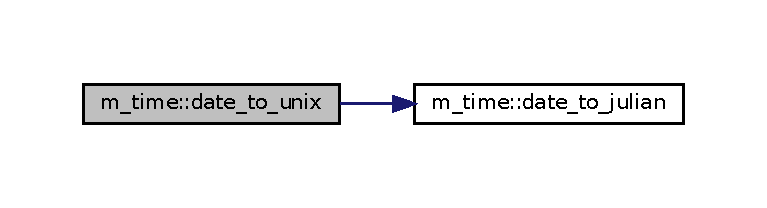
\includegraphics[width=350pt]{namespacem__time_aed245c691853279ebf0ce899dec9caa9_cgraph}
\end{center}
\end{figure}
Here is the caller graph for this function\+:\nopagebreak
\begin{figure}[H]
\begin{center}
\leavevmode
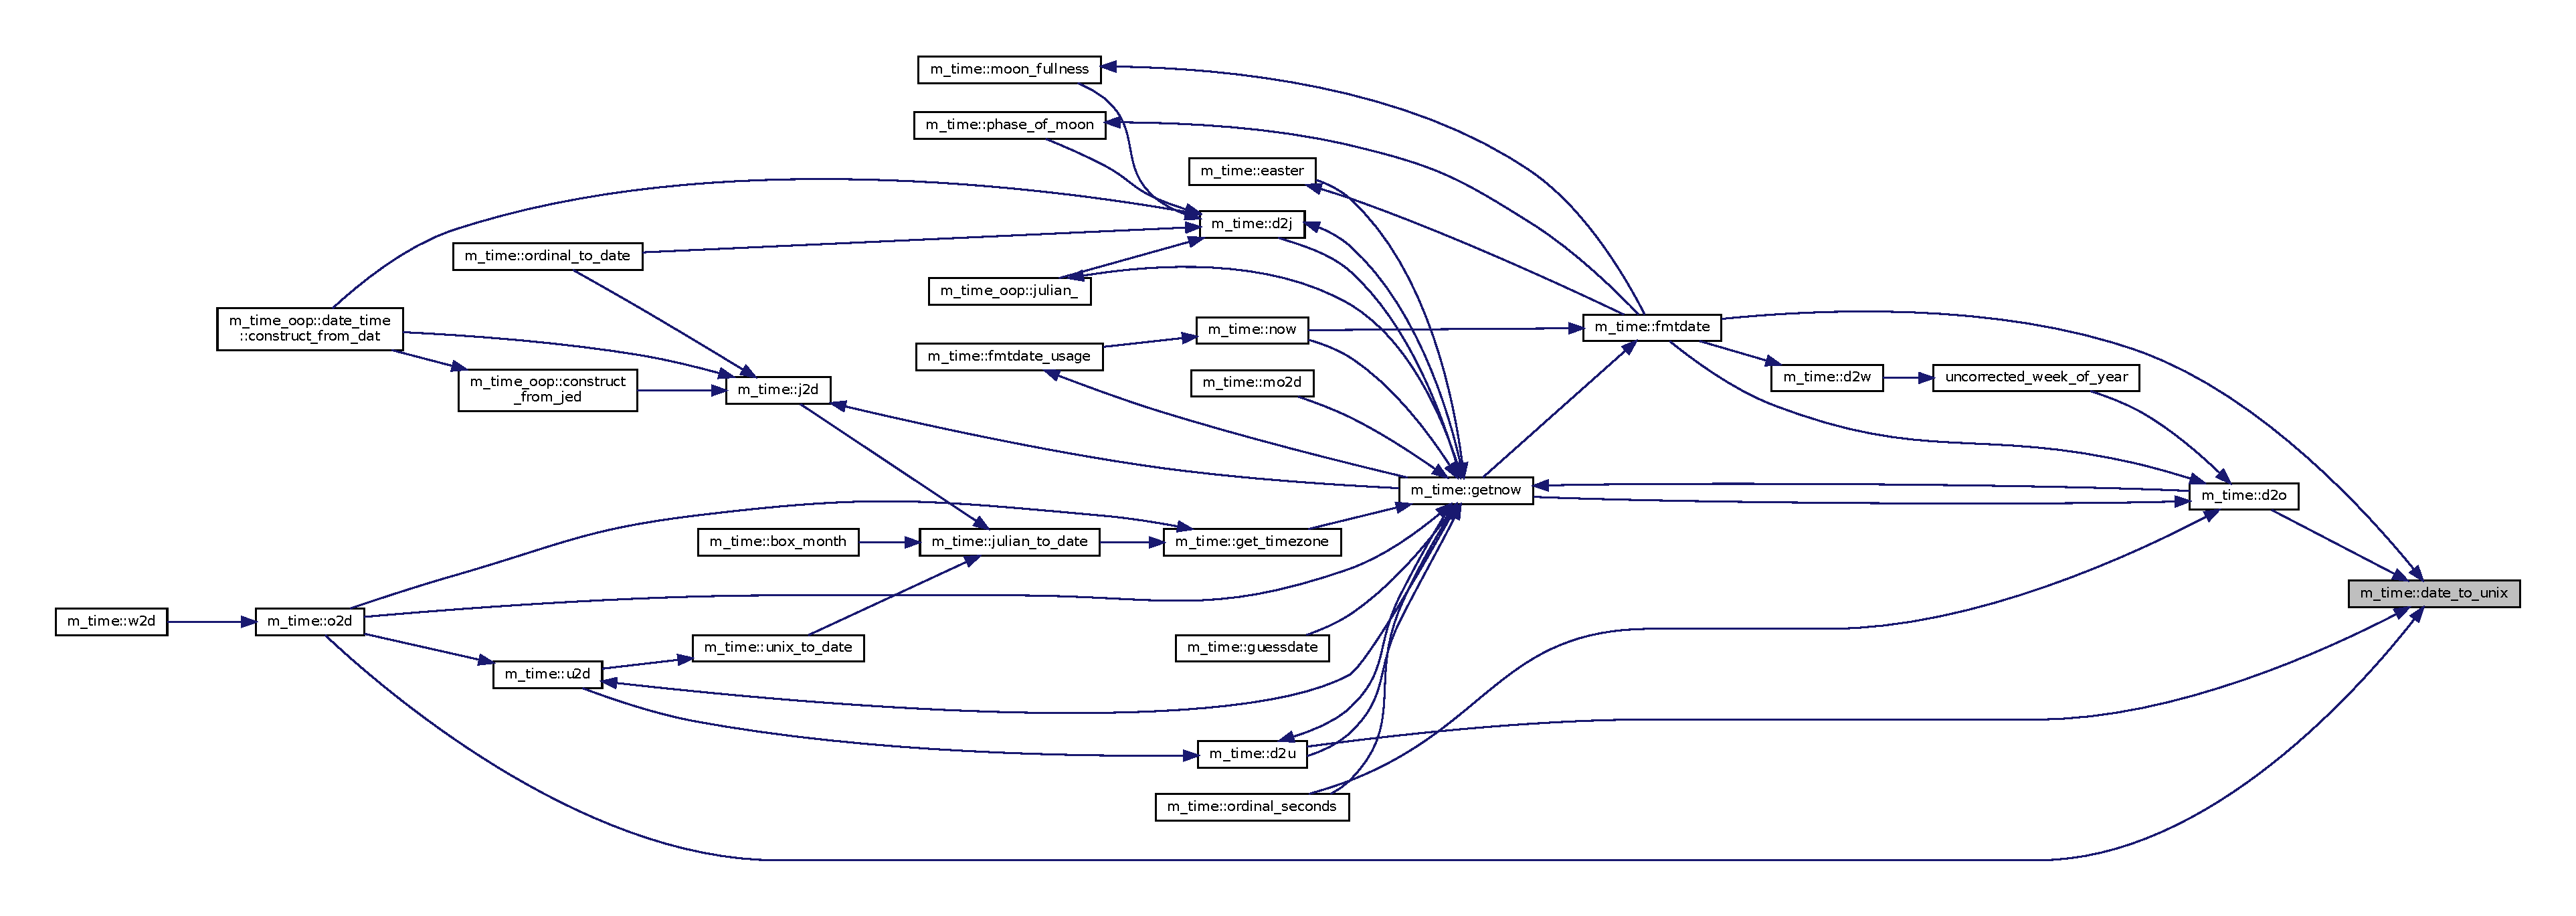
\includegraphics[width=350pt]{namespacem__time_aed245c691853279ebf0ce899dec9caa9_icgraph}
\end{center}
\end{figure}
\mbox{\Hypertarget{namespacem__time_a99393c7906f1989f90ece03969224938}\label{namespacem__time_a99393c7906f1989f90ece03969224938}} 
\index{m\_time@{m\_time}!days2sec@{days2sec}}
\index{days2sec@{days2sec}!m\_time@{m\_time}}
\doxysubsubsection{\texorpdfstring{days2sec()}{days2sec()}}
{\footnotesize\ttfamily real(kind=\mbox{\hyperlink{namespacem__time_ac10ea9e8d59ec74eaa7d89f2517d7422}{realtime}}) function, public m\+\_\+time\+::days2sec (\begin{DoxyParamCaption}\item[{character(len=$\ast$), intent(in)}]{str }\end{DoxyParamCaption})}

\hypertarget{namespacem__time_autotoc_md200}{}\doxysubsubsection{N\+A\+ME}\label{namespacem__time_autotoc_md200}
days2sec(3f) -\/ \mbox{[}M\+\_\+time\+:D\+U\+R\+A\+T\+I\+ON\mbox{]} convert string of form \mbox{[}\mbox{[}-\/\mbox{]}dd-\/\mbox{]}hh\+:mm\+:ss.\+nn to seconds (L\+I\+C\+E\+N\+SE\+:PD)\hypertarget{namespacem__time_autotoc_md201}{}\doxysubsubsection{S\+Y\+N\+O\+P\+S\+IS}\label{namespacem__time_autotoc_md201}
\begin{DoxyVerb}function days2sec(str) result(time)

 character(len=*),intent(in)       :: str
 real(kind=realtime)               :: time
\end{DoxyVerb}
\hypertarget{namespacem__time_autotoc_md202}{}\doxysubsubsection{D\+E\+S\+C\+R\+I\+P\+T\+I\+ON}\label{namespacem__time_autotoc_md202}
Given a string representing a duration of the form \char`\"{}\mbox{[}-\/\mbox{]}\mbox{[}\mbox{[}\mbox{[}dd-\/\mbox{]}hh\+:\mbox{]}mm\+:\mbox{]}ss\char`\"{} or \mbox{[}N\+Nd\mbox{]}\mbox{[}N\+Nh\mbox{]}\mbox{[}N\+Nm\mbox{[}\mbox{]}N\+Ns\mbox{]}\mbox{[}N\+Nw\mbox{]} return a value representing seconds.

If \char`\"{}dd-\/\char`\"{} is present, units for the numbers are assumed to proceed from day to hour to minute to second. But if no day is present, the units are assumed to proceed from second to minutes to hour from left to right. That is ... \begin{DoxyVerb}  [-]dd-hh:mm:ss
  [-]dd-hh:mm
  [-]dd-hh

  hh:mm:ss
  mm:ss
  ss

  Where dd is days, hh hours, mm minutes and ss seconds.
\end{DoxyVerb}


A decimal fraction is supported on the seconds (Actually, any of the numeric values may represent positive floating point numbers). Spaces are ignored.

Simple numeric values may also be used with unit suffixes; where s,m,h, or d represents seconds, minutes, hours or days and w represents a week. Allowed aliases for w,d,h,m, and s units are \begin{DoxyVerb} [NNd][NNh][NNm][NNs][NNw]

   d -  days,day
   m -  minutes,minute,min,mins
   h -  hours,hour,hr,hrs
   s -  seconds,second,sec,secs
   w -  week, weeks, wk, wks
\end{DoxyVerb}


The numeric values may represent floating point numbers.

Spaces, commas and case are ignored.\hypertarget{namespacem__time_autotoc_md203}{}\doxysubsubsection{O\+P\+T\+I\+O\+NS}\label{namespacem__time_autotoc_md203}
str string of the general form dd-\/hh\+:mm\+:ss.\+nn \hypertarget{namespacem__time_autotoc_md204}{}\doxysubsubsection{R\+E\+T\+U\+R\+NS}\label{namespacem__time_autotoc_md204}
time the number of seconds represented by the input string\hypertarget{namespacem__time_autotoc_md205}{}\doxysubsubsection{E\+X\+A\+M\+P\+LE}\label{namespacem__time_autotoc_md205}
\begin{DoxyVerb}Sample program:

 program demo_days2sec
 use M_time, only : days2sec
 implicit none
    write(*,*)days2sec('1-12:04:20')
    write(*,*)'one second ',days2sec('1')
    write(*,*)'one minute ',days2sec('1:00')
    write(*,*)'one hour ',days2sec('1:00:00')
    write(*,*)'one day ',days2sec('1-00:00:00')
    write(*,*)nint(days2sec(' 1-12:04:20              ')) .eq. 129860
    write(*,*)nint(days2sec(' 1.5 days                ')) .eq. 129600
    write(*,*)nint(days2sec(' 1.5 days 4hrs 30minutes ')) .eq. 145800
    write(*,*)nint(days2sec(' 1.5d                    ')) .eq. 129600
    write(*,*)nint(days2sec(' 1d2h3m4s                ')) .eq. 93784
    ! duplicates
    write(*,*)nint(days2sec(' 1d1d1d                  ')) .eq. 259200
    ! negative values
    write(*,*)nint(days2sec(' 4d-12h                  ')) .eq. 302400
 end program demo_days2sec

Results:

 > 129860.00000000000
 > one second    1.0000000000000000
 > one minute    60.000000000000000
 > one hour    3600.0000000000000
 > one day    86400.000000000000
 > T
 > T
 > T
 > T
 > T
 > T
 > T
\end{DoxyVerb}
\hypertarget{namespacem__time_autotoc_md206}{}\doxysubsubsection{A\+U\+T\+H\+OR}\label{namespacem__time_autotoc_md206}
John S. Urban, 2015 \hypertarget{namespacem__time_autotoc_md207}{}\doxysubsubsection{L\+I\+C\+E\+N\+SE}\label{namespacem__time_autotoc_md207}
Public Domain 

References m\+\_\+time\+\_\+duplicate\+::compact(), m\+\_\+time\+\_\+duplicate\+::lower(), m\+\_\+time\+\_\+duplicate\+::s2v(), m\+\_\+time\+\_\+duplicate\+::split(), m\+\_\+time\+\_\+duplicate\+::substitute(), and m\+\_\+time\+\_\+duplicate\+::transliterate().

Here is the call graph for this function\+:\nopagebreak
\begin{figure}[H]
\begin{center}
\leavevmode
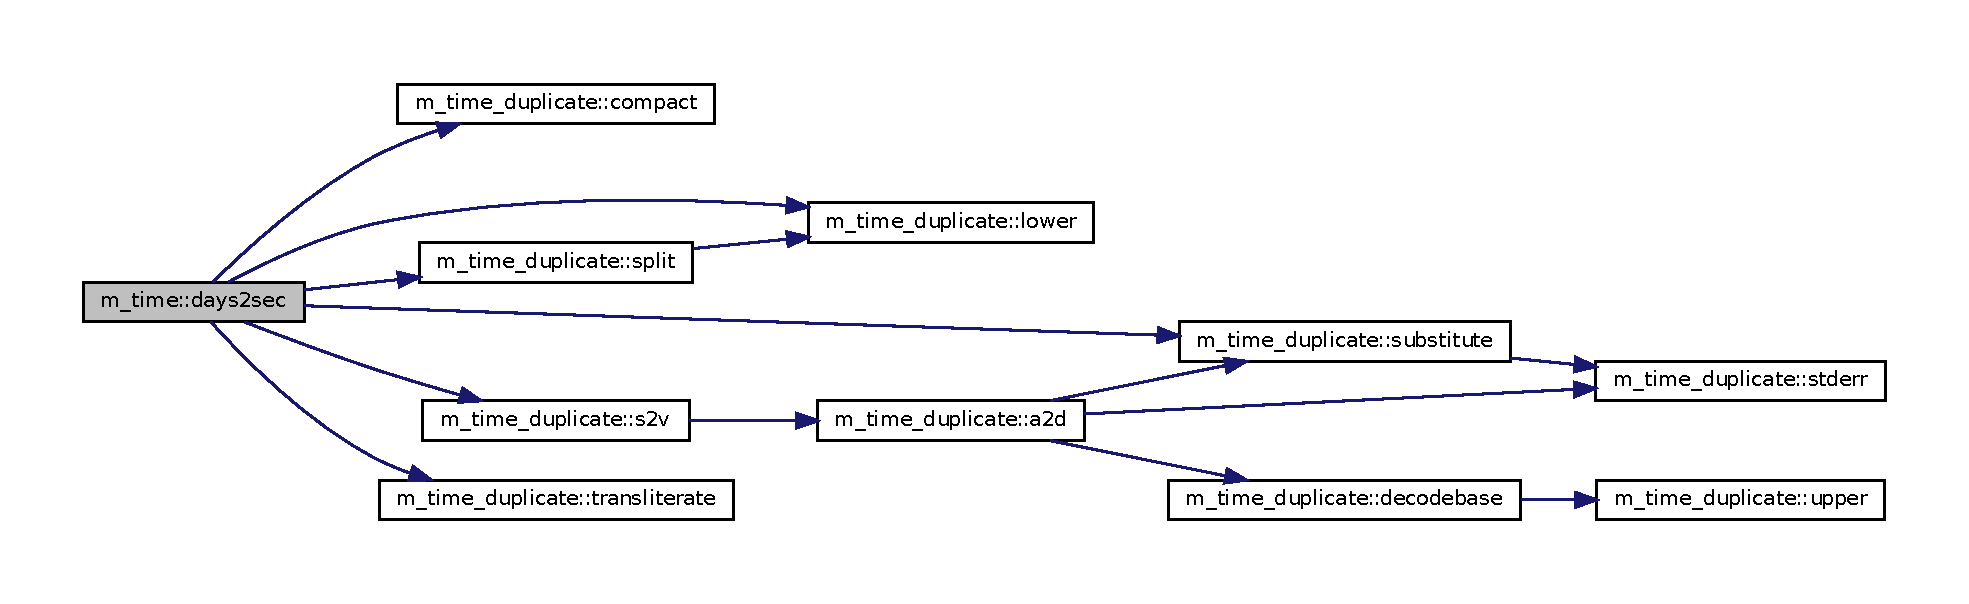
\includegraphics[width=350pt]{namespacem__time_a99393c7906f1989f90ece03969224938_cgraph}
\end{center}
\end{figure}
\mbox{\Hypertarget{namespacem__time_adfda8a89820b8d0ad4581a14896e4ce5}\label{namespacem__time_adfda8a89820b8d0ad4581a14896e4ce5}} 
\index{m\_time@{m\_time}!dow@{dow}}
\index{dow@{dow}!m\_time@{m\_time}}
\doxysubsubsection{\texorpdfstring{dow()}{dow()}}
{\footnotesize\ttfamily subroutine, public m\+\_\+time\+::dow (\begin{DoxyParamCaption}\item[{integer, dimension(8), intent(in)}]{values,  }\item[{integer, intent(out), optional}]{weekday,  }\item[{character(len=$\ast$), intent(out), optional}]{day,  }\item[{integer, intent(out), optional}]{ierr }\end{DoxyParamCaption})}

\hypertarget{namespacem__time_autotoc_md115}{}\doxysubsubsection{N\+A\+ME}\label{namespacem__time_autotoc_md115}
dow(3f) -\/ \mbox{[}M\+\_\+time\+:D\+A\+Y\+\_\+\+O\+F\+\_\+\+W\+E\+EK\mbox{]} given a date-\/time array D\+AT return the day of the week (L\+I\+C\+E\+N\+SE\+:PD)\hypertarget{namespacem__time_autotoc_md116}{}\doxysubsubsection{S\+Y\+N\+O\+P\+S\+IS}\label{namespacem__time_autotoc_md116}
\begin{DoxyVerb}subroutine dow(values, weekday, day, ierr)

 integer,intent(in) :: values(8)
 integer,intent(out),optional :: weekday
 character(len=*),intent(out),optional :: day
 integer,intent(out),optional :: ierr
\end{DoxyVerb}
\hypertarget{namespacem__time_autotoc_md117}{}\doxysubsubsection{D\+E\+S\+C\+R\+I\+P\+T\+I\+ON}\label{namespacem__time_autotoc_md117}
Given a date array D\+AT return the day of the week as a number and a name, Mon=1.\hypertarget{namespacem__time_autotoc_md118}{}\doxysubsubsection{O\+P\+T\+I\+O\+NS}\label{namespacem__time_autotoc_md118}
values \char`\"{}\+D\+A\+T\char`\"{} array (an integer array of the same format as the array returned by the intrinsic D\+A\+T\+E\+\_\+\+A\+N\+D\+\_\+\+T\+I\+M\+E(3f)) describing the date to be used to calculate the day of the week. \hypertarget{namespacem__time_autotoc_md119}{}\doxysubsubsection{R\+E\+T\+U\+R\+NS}\label{namespacem__time_autotoc_md119}
weekday The numeric day of the week, starting with Monday=1. Optional. day The name of the day of the week. Optional. ierr Error code \begin{DoxyVerb}     o [ 0] correct
     o [-1] invalid input date
     o [-2] neither day nor weekday
       return values were requested.

     If the error code is not returned and an error occurs,
     the program is stopped.
\end{DoxyVerb}
\hypertarget{namespacem__time_autotoc_md120}{}\doxysubsubsection{E\+X\+A\+M\+P\+LE}\label{namespacem__time_autotoc_md120}
\begin{DoxyVerb}Sample program:

 program demo_dow
 use M_time, only : dow
 implicit none
 integer          :: dat(8)     ! input date array
 integer          :: weekday
 character(len=9) :: day
 integer          :: ierr
   call date_and_time(values=dat)
   call dow(dat, weekday, day, ierr)
   write(*,'(a,i0)')'weekday=',weekday
   write(*,'(a,a)')'day=',trim(day)
   write(*,'(a,i0)')'ierr=',ierr
 end program demo_dow

results:

 weekday=1
 day=Monday
 ierr=0
\end{DoxyVerb}
 \hypertarget{namespacem__time_autotoc_md121}{}\doxysubsubsection{A\+U\+T\+H\+OR}\label{namespacem__time_autotoc_md121}
John S. Urban, 2015-\/12-\/19 \hypertarget{namespacem__time_autotoc_md122}{}\doxysubsubsection{L\+I\+C\+E\+N\+SE}\label{namespacem__time_autotoc_md122}
Public Domain 

References date\+\_\+to\+\_\+julian().

Here is the call graph for this function\+:\nopagebreak
\begin{figure}[H]
\begin{center}
\leavevmode
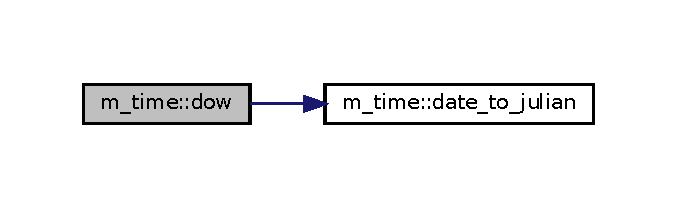
\includegraphics[width=325pt]{namespacem__time_adfda8a89820b8d0ad4581a14896e4ce5_cgraph}
\end{center}
\end{figure}
Here is the caller graph for this function\+:\nopagebreak
\begin{figure}[H]
\begin{center}
\leavevmode
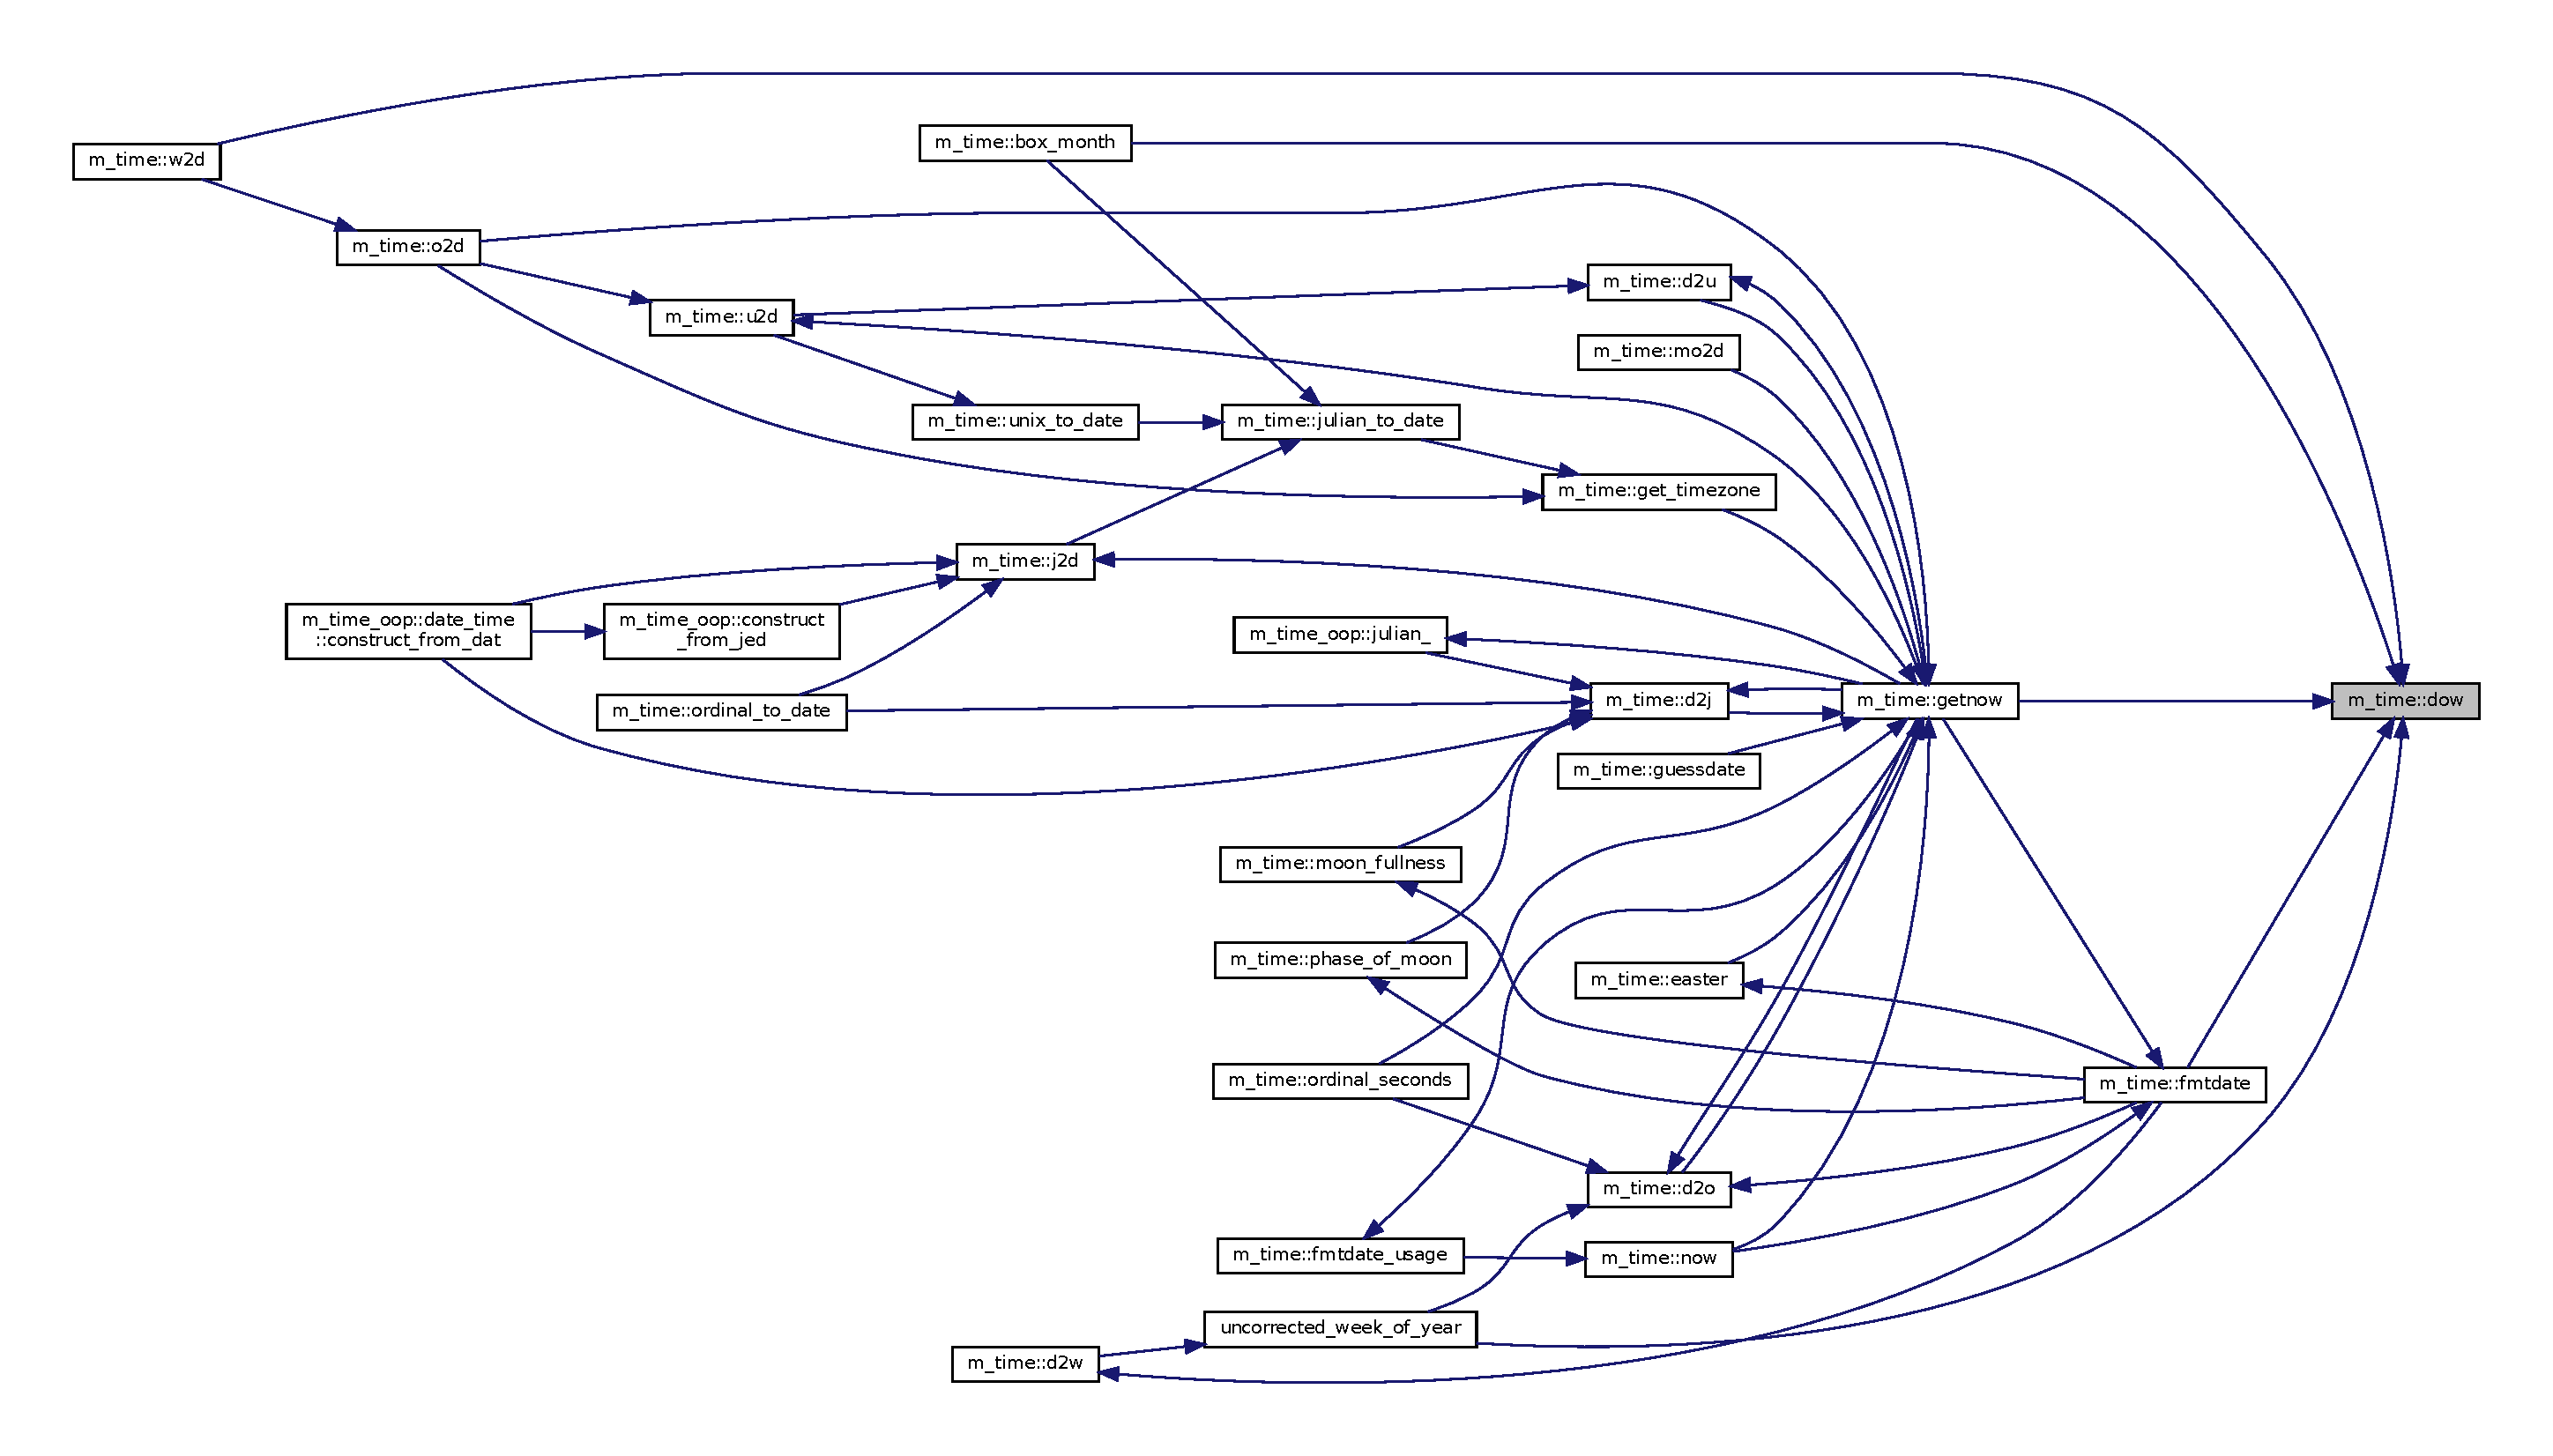
\includegraphics[width=350pt]{namespacem__time_adfda8a89820b8d0ad4581a14896e4ce5_icgraph}
\end{center}
\end{figure}
\mbox{\Hypertarget{namespacem__time_a5ccb70e20160fcf26bb403dbff1f138a}\label{namespacem__time_a5ccb70e20160fcf26bb403dbff1f138a}} 
\index{m\_time@{m\_time}!easter@{easter}}
\index{easter@{easter}!m\_time@{m\_time}}
\doxysubsubsection{\texorpdfstring{easter()}{easter()}}
{\footnotesize\ttfamily subroutine, public m\+\_\+time\+::easter (\begin{DoxyParamCaption}\item[{integer, intent(in)}]{year,  }\item[{integer, dimension(8), intent(out)}]{dat }\end{DoxyParamCaption})}

\hypertarget{namespacem__time_autotoc_md222}{}\doxysubsubsection{N\+A\+ME}\label{namespacem__time_autotoc_md222}
easter(3f) -\/ \mbox{[}M\+\_\+time\+:A\+S\+T\+R\+O\+L\+O\+G\+I\+C\+AL\mbox{]} calculate date for Easter given a year (L\+I\+C\+E\+N\+SE\+:PD)\hypertarget{namespacem__time_autotoc_md223}{}\doxysubsubsection{S\+Y\+N\+O\+P\+S\+IS}\label{namespacem__time_autotoc_md223}
subroutine easter(year,dat)

integer, intent(in) \+:: year integer, intent(out) \+:: dat\hypertarget{namespacem__time_autotoc_md224}{}\doxysubsubsection{D\+E\+S\+C\+R\+I\+P\+T\+I\+ON}\label{namespacem__time_autotoc_md224}
The Date of Easter (Sunday)

The algorithm is due to J.-\/M. Oudin (1940) and is reprinted in the Explanatory Supplement to the Astronomical Almanac, ed. P. K. Seidelmann (1992). See Chapter 12, \char`\"{}\+Calendars\char`\"{}, by L. E. Doggett.

The following are dates of Easter from 1980 to 2024\+: \begin{DoxyVerb} 1980  April  6        1995  April 16        2010  April  4
 1981  April 19        1996  April  7        2011  April 24
 1982  April 11        1997  March 30        2012  April  8
 1983  April  3        1998  April 12        2013  March 31
 1984  April 22        1999  April  4        2014  April 20
 1985  April  7        2000  April 23        2015  April  5
 1986  March 30        2001  April 15        2016  March 27
 1987  April 19        2002  March 31        2017  April 16
 1988  April  3        2003  April 20        2018  April  1
 1989  March 26        2004  April 11        2019  April 21
 1990  April 15        2005  March 27        2020  April 12
 1991  March 31        2006  April 16        2021  April  4
 1992  April 19        2007  April  8        2022  April 17
 1993  April 11        2008  March 23        2023  April  9
 1994  April  3        2009  April 12        2024  March 31
\end{DoxyVerb}


N.\+B. The date of Easter for the Eastern Orthodox Church may be different.\hypertarget{namespacem__time_autotoc_md225}{}\doxysubsubsection{O\+P\+T\+I\+O\+NS}\label{namespacem__time_autotoc_md225}
year Year for which to calculate day that Easter falls on \hypertarget{namespacem__time_autotoc_md226}{}\doxysubsubsection{R\+E\+S\+U\+L\+TS}\label{namespacem__time_autotoc_md226}
dat Date array for noon on Easter for the specified year\hypertarget{namespacem__time_autotoc_md227}{}\doxysubsubsection{E\+X\+A\+M\+P\+LE}\label{namespacem__time_autotoc_md227}
\begin{DoxyVerb}Sample program:

 program demo_easter
 use M_time, only : easter, fmtdate
 implicit none
 integer :: year
 integer :: dat(8) ! year,month,day,tz,hour,minute,second,millisecond
   call date_and_time(values=dat)  ! get current year
   year=dat(1)
   call easter(year, dat)
   write(*,*)fmtdate(dat,&
   "Easter day: the %d day of %L in the year of our Lord %Y")
 end program demo_easter

Sample output:

 Easter day: the 16th day of April in the year of our Lord 2017
\end{DoxyVerb}


U.\+S. Naval Observatory Astronomical Applications Department

This code assembled by Alan Miller Reference web site\+: \href{http://aa.usno.navy.mil/faq/docs/easter.html}{\texttt{ http\+://aa.\+usno.\+navy.\+mil/faq/docs/easter.\+html}} Latest revision 8 April 2002 Here is the caller graph for this function\+:\nopagebreak
\begin{figure}[H]
\begin{center}
\leavevmode
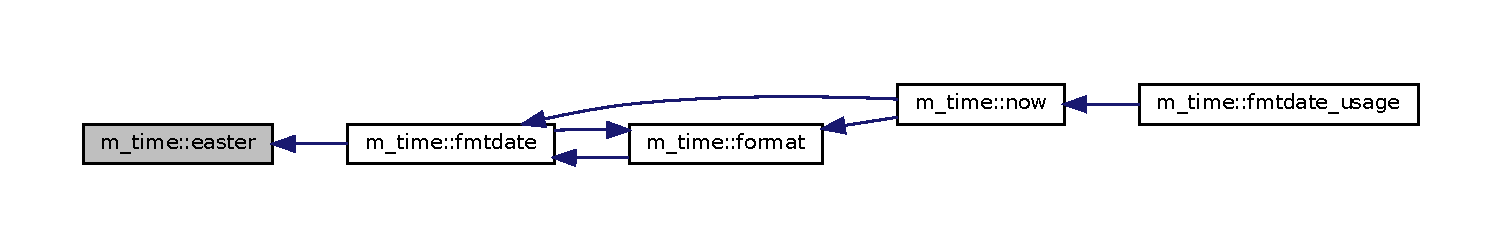
\includegraphics[width=350pt]{namespacem__time_a5ccb70e20160fcf26bb403dbff1f138a_icgraph}
\end{center}
\end{figure}
\mbox{\Hypertarget{namespacem__time_a2cb84c9b8af4f395b76aed76e1431328}\label{namespacem__time_a2cb84c9b8af4f395b76aed76e1431328}} 
\index{m\_time@{m\_time}!fmtdate@{fmtdate}}
\index{fmtdate@{fmtdate}!m\_time@{m\_time}}
\doxysubsubsection{\texorpdfstring{fmtdate()}{fmtdate()}}
{\footnotesize\ttfamily character(len=\+:) function, allocatable, public m\+\_\+time\+::fmtdate (\begin{DoxyParamCaption}\item[{integer, dimension(8), intent(in)}]{values,  }\item[{character(len=$\ast$), intent(in), optional}]{format }\end{DoxyParamCaption})}

\hypertarget{namespacem__time_autotoc_md94}{}\doxysubsubsection{N\+A\+ME}\label{namespacem__time_autotoc_md94}
fmtdate(3f) -\/ \mbox{[}M\+\_\+time\+:D\+A\+T\+E\+\_\+\+P\+R\+I\+N\+T\+I\+NG\mbox{]} given D\+AT date-\/time array return date as string using specified format (L\+I\+C\+E\+N\+SE\+:PD)\hypertarget{namespacem__time_autotoc_md95}{}\doxysubsubsection{S\+Y\+N\+O\+P\+S\+IS}\label{namespacem__time_autotoc_md95}
\begin{DoxyVerb}function fmtdate(values,format) RESULT (timestr)

 integer,dimension(8),intent(in)      :: values
 character(len=*),intent(in),optional :: format
 character(len=:),allocatable         :: timestr
\end{DoxyVerb}
\hypertarget{namespacem__time_autotoc_md96}{}\doxysubsubsection{D\+E\+S\+C\+R\+I\+P\+T\+I\+ON}\label{namespacem__time_autotoc_md96}
The fmtdate(3f) procedure lets you reformat a D\+AT array in many common formats using a special string containing macro names beginning with \textquotesingle{}\textquotesingle{}. To see the allowable macros call or see the fmtdate\+\_\+usage(3f) routine.\hypertarget{namespacem__time_autotoc_md97}{}\doxysubsubsection{O\+P\+T\+I\+O\+NS}\label{namespacem__time_autotoc_md97}
values date in a \char`\"{}\+D\+A\+T\char`\"{} array, which is the same format as the values returned by the intrinsic D\+A\+T\+E\+\_\+\+A\+N\+D\+\_\+\+T\+I\+M\+E(3f)\+:

dat=\mbox{[} year,month,day,timezone,hour,\& \& minutes,seconds,milliseconds\mbox{]}

format string describing how to format the \char`\"{}\+D\+A\+T\char`\"{} array. For a complete description of the formatting macros supported see fmtdate\+\_\+usage(3f). \hypertarget{namespacem__time_autotoc_md98}{}\doxysubsubsection{R\+E\+T\+U\+R\+NS}\label{namespacem__time_autotoc_md98}
timestr formatted output string representing date\hypertarget{namespacem__time_autotoc_md99}{}\doxysubsubsection{E\+X\+A\+M\+P\+LE}\label{namespacem__time_autotoc_md99}
\begin{DoxyVerb}Sample program:

 program demo_fmtdate
 use M_time, only : fmtdate
 implicit none
 integer :: dat(8)
    call date_and_time(values=dat)
    write(*,*)fmtdate(dat,"current date: %w, %l %d, %Y %H:%m:%s %N")
    call showme()
 contains
 subroutine showme()
    use M_time, only : fmtdate_usage
    call fmtdate_usage() ! see all formatting options
 end subroutine showme
 end program demo_fmtdate

results:

   The current date is Sun, Jul 17th, 2016 01:21:35 PM
    ::
    :: An up-to-date description of all the
    :: formatting options will appear here
    ::
\end{DoxyVerb}
\hypertarget{namespacem__time_autotoc_md100}{}\doxysubsubsection{A\+U\+T\+H\+OR}\label{namespacem__time_autotoc_md100}
John S. Urban, 2015-\/12-\/19 \hypertarget{namespacem__time_autotoc_md101}{}\doxysubsubsection{L\+I\+C\+E\+N\+SE}\label{namespacem__time_autotoc_md101}
Public Domain 

References d2o(), d2w(), date\+\_\+to\+\_\+julian(), date\+\_\+to\+\_\+unix(), dow(), easter(), moon\+\_\+fullness(), phase\+\_\+of\+\_\+moon(), m\+\_\+time\+\_\+duplicate\+::substitute(), and v2mo().

Here is the call graph for this function\+:\nopagebreak
\begin{figure}[H]
\begin{center}
\leavevmode
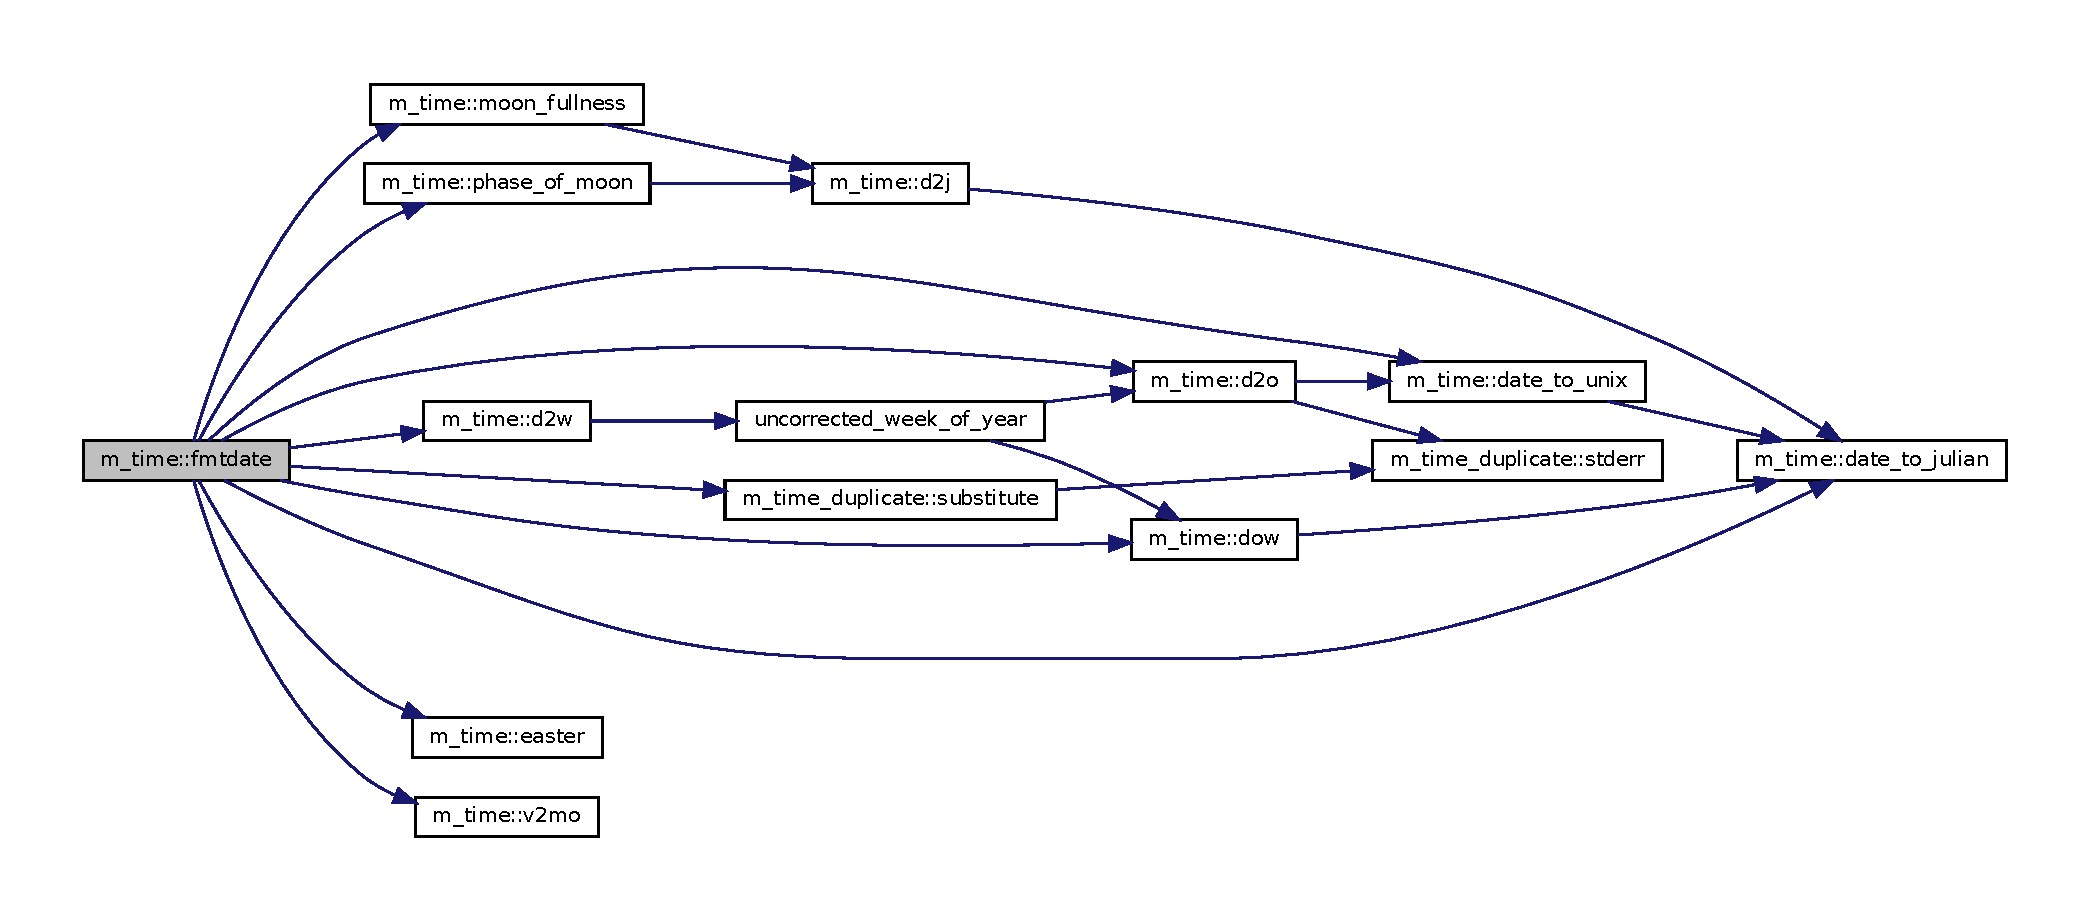
\includegraphics[width=350pt]{namespacem__time_a2cb84c9b8af4f395b76aed76e1431328_cgraph}
\end{center}
\end{figure}
Here is the caller graph for this function\+:\nopagebreak
\begin{figure}[H]
\begin{center}
\leavevmode
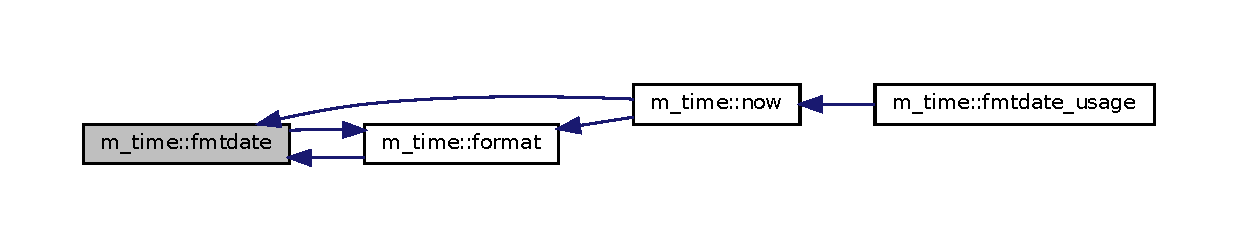
\includegraphics[width=350pt]{namespacem__time_a2cb84c9b8af4f395b76aed76e1431328_icgraph}
\end{center}
\end{figure}
\mbox{\Hypertarget{namespacem__time_a914927f70fb9495af1be2e484b967111}\label{namespacem__time_a914927f70fb9495af1be2e484b967111}} 
\index{m\_time@{m\_time}!fmtdate\_usage@{fmtdate\_usage}}
\index{fmtdate\_usage@{fmtdate\_usage}!m\_time@{m\_time}}
\doxysubsubsection{\texorpdfstring{fmtdate\_usage()}{fmtdate\_usage()}}
{\footnotesize\ttfamily subroutine, public m\+\_\+time\+::fmtdate\+\_\+usage (\begin{DoxyParamCaption}\item[{integer, intent(in), optional}]{indent }\end{DoxyParamCaption})}

\hypertarget{namespacem__time_autotoc_md102}{}\doxysubsubsection{N\+A\+ME}\label{namespacem__time_autotoc_md102}
fmtdate\+\_\+usage(3f) -\/ \mbox{[}M\+\_\+time\+:D\+A\+T\+E\+\_\+\+P\+R\+I\+N\+T\+I\+NG\mbox{]} display macros recognized by fmtdate(3f) and now(3f) (L\+I\+C\+E\+N\+SE\+:PD)\hypertarget{namespacem__time_autotoc_md103}{}\doxysubsubsection{S\+Y\+N\+O\+P\+S\+IS}\label{namespacem__time_autotoc_md103}
\begin{DoxyVerb}subroutine fmtdate_usage(indent)

 integer,intent(in),optional      :: indent
\end{DoxyVerb}
\hypertarget{namespacem__time_autotoc_md104}{}\doxysubsubsection{D\+E\+S\+C\+R\+I\+P\+T\+I\+ON}\label{namespacem__time_autotoc_md104}
The fmtdate\+\_\+usage(3f) subroutine displays the formatting options available for use in procedures such as fmtdate(3f) and now(3f). It is typically used to produce up-\/to-\/date help text in commands that use the M\+\_\+time(3fm) module, so that the formatting information only needs maintained in one place (this routine) and is easily displayed so users can quickly obtain a description of the formatting macros.\hypertarget{namespacem__time_autotoc_md105}{}\doxysubsubsection{O\+P\+T\+I\+O\+NS}\label{namespacem__time_autotoc_md105}
indent how many spaces to prefix the output with, so that calling programs can position the output. Default for this optional parameter is three (3).\hypertarget{namespacem__time_autotoc_md106}{}\doxysubsubsection{E\+X\+A\+M\+P\+LE}\label{namespacem__time_autotoc_md106}
\begin{DoxyVerb}Sample Program:

 program demo_fmtdate_usage
 use M_time, only : fmtdate_usage
 implicit none
    call fmtdate_usage() ! see all formatting options
 end program demo_fmtdate_usage

results (actually call the routine to ensure this is up to date):

 Description                                        Example

 Base time array:
 (1) %Y -- year, yyyy                                2016
 (2) %M -- month of year, 01 to 12                   07
 (3) %D -- day of month, 01 to 31                    29
     %d -- day of month, with suffix (1st, 2nd,...)  29th
 (4) %Z -- minutes from UTC                          -0240
     %z -- -+hh:mm from UTC                          -04:00
     %T -- -+hhmm  from UTC                          -0400
 (5) %h -- hours, 00 to 23                           10
     %H -- hour (1 to 12, or twelve-hour clock)      10
     %N -- midnight< AM <=noon; noon<= PM <midnight  AM
 (6) %m -- minutes, 00 to 59                         54
 (7) %s -- sec, 00 to 59                             08
 (8) %x -- milliseconds 000 to 999                   521
 Conversions:
     %E -- Unix Epoch time                           1469804048.5220029
     %e -- integer value of Unix Epoch time          1469804049
     %J -- Julian  date                              2457599.121
     %j -- integer value of Julian Date(Julian Day)  2457599
     %O -- Ordinal day (day of year)                 211
     %o -- Whole days since Unix Epoch date          17011
     %U -- day of week, 1..7 Sunday=1                6
     %u -- day of week, 1..7 Monday=1                5
     %i -- ISO week of year 1..53                    30
     %I -- iso-8601 week-numbering date(yyyy-Www-d)  2016-W30-5
  Names:
     %l -- abbreviated month name                    Jul
     %L -- full month name                           July
     %w -- first three characters of weekday         Fri
     %W -- weekday name                              Friday
     %p -- phase of moon                             New
     %P -- percent of way from new to full moon      -1%
  Literals:
     %% -- a literal %                               %
     %t -- tab character
     %b -- blank character
     %B -- exclamation(bang) character
     %n -- new line (system dependent)
     %q -- single quote (apostrophe)
     %Q -- double quote
  Program timing:
     %c -- CPU_TIME(3f) output                     .21875000000000000
     %C -- number of times this routine is used    1
     %S -- seconds since last use of this format   .0000000000000000
     %k -- time in seconds from SYSTEM_CLOCK(3f)   723258.812
     %K -- time in clicks from SYSTEM_CLOCK(3f)    723258812

If no percent (%) is found in the format one of several
alternate substitutions occurs.

If the format is composed entirely of one of the following
keywords the following substitutions occur:

  "iso-8601",
  "iso"        ==> %Y-%M-%DT%h:%m:%s%z
  "iso-8601W",
  "isoweek"    ==> %I 2016-W30-5
  "sql"        ==> "%Y-%M-%D %h:%m:%s.%x"
  "sqlday"     ==> "%Y-%M-%D"
  "sqltime"    ==> "%h:%m:%s.%x"
  "rfc-2822"   ==> %w, %D %l %Y %h:%m:%s %T
  "rfc-3339"   ==> %Y-%M-%DT%h:%m:%s%z
  "date"       ==> %w %l %D %h:%m:%s UTC%z %Y
  "short"      ==> %w, %l %d, %Y %H:%m:%s %N UTC%z
  "long"," "   ==> %W, %L %d, %Y %H:%m:%s %N UTC%z
  "suffix"     ==> %Y%D%M%h%m%s
  "formal"     ==> The %d of %L %Y
  "lord"       ==> the %d day of %L in the year of our Lord %Y
  "easter"     ==> FOR THE YEAR OF THE CURRENT DATE:
                   Easter day: the %d day of %L in the year of our Lord %Y
  "all"        ==> A SAMPLE OF DATE FORMATS

otherwise the following words are replaced with the most
common macros:

numeric values:

   year     %Y  2016
   month    %M  07
   day      %D  29
   hour     %h  10
   minute   %m  54
   second   %s  08
   timezone %T  0400

   epoch    %e  1469804049
   julian   %j  2457599
   ordinal  %O  211
   weekday  %u  5

string values:

   MONTH    %L  July
   Month    %l  Jul
   WEEKDAY  %W  Thursday
   Weekday  %w  Thu
   DAY      %d  7th
   TIMEZONE %z  -04:00
   Timezone %Z  -240
   GOOD     %N  AM
   HOUR     %H  10

if none of these keywords are found then every letter that
is a macro is assumed to have an implied percent in front
of it. For example:

   YMDhms ==> %Y%M%D%h%m%s ==> 20160729105408
\end{DoxyVerb}
 \hypertarget{namespacem__time_autotoc_md107}{}\doxysubsubsection{A\+U\+T\+H\+OR}\label{namespacem__time_autotoc_md107}
John S. Urban, 2015-\/10-\/24 \hypertarget{namespacem__time_autotoc_md108}{}\doxysubsubsection{L\+I\+C\+E\+N\+SE}\label{namespacem__time_autotoc_md108}
Public Domain 

References now().

Here is the call graph for this function\+:\nopagebreak
\begin{figure}[H]
\begin{center}
\leavevmode
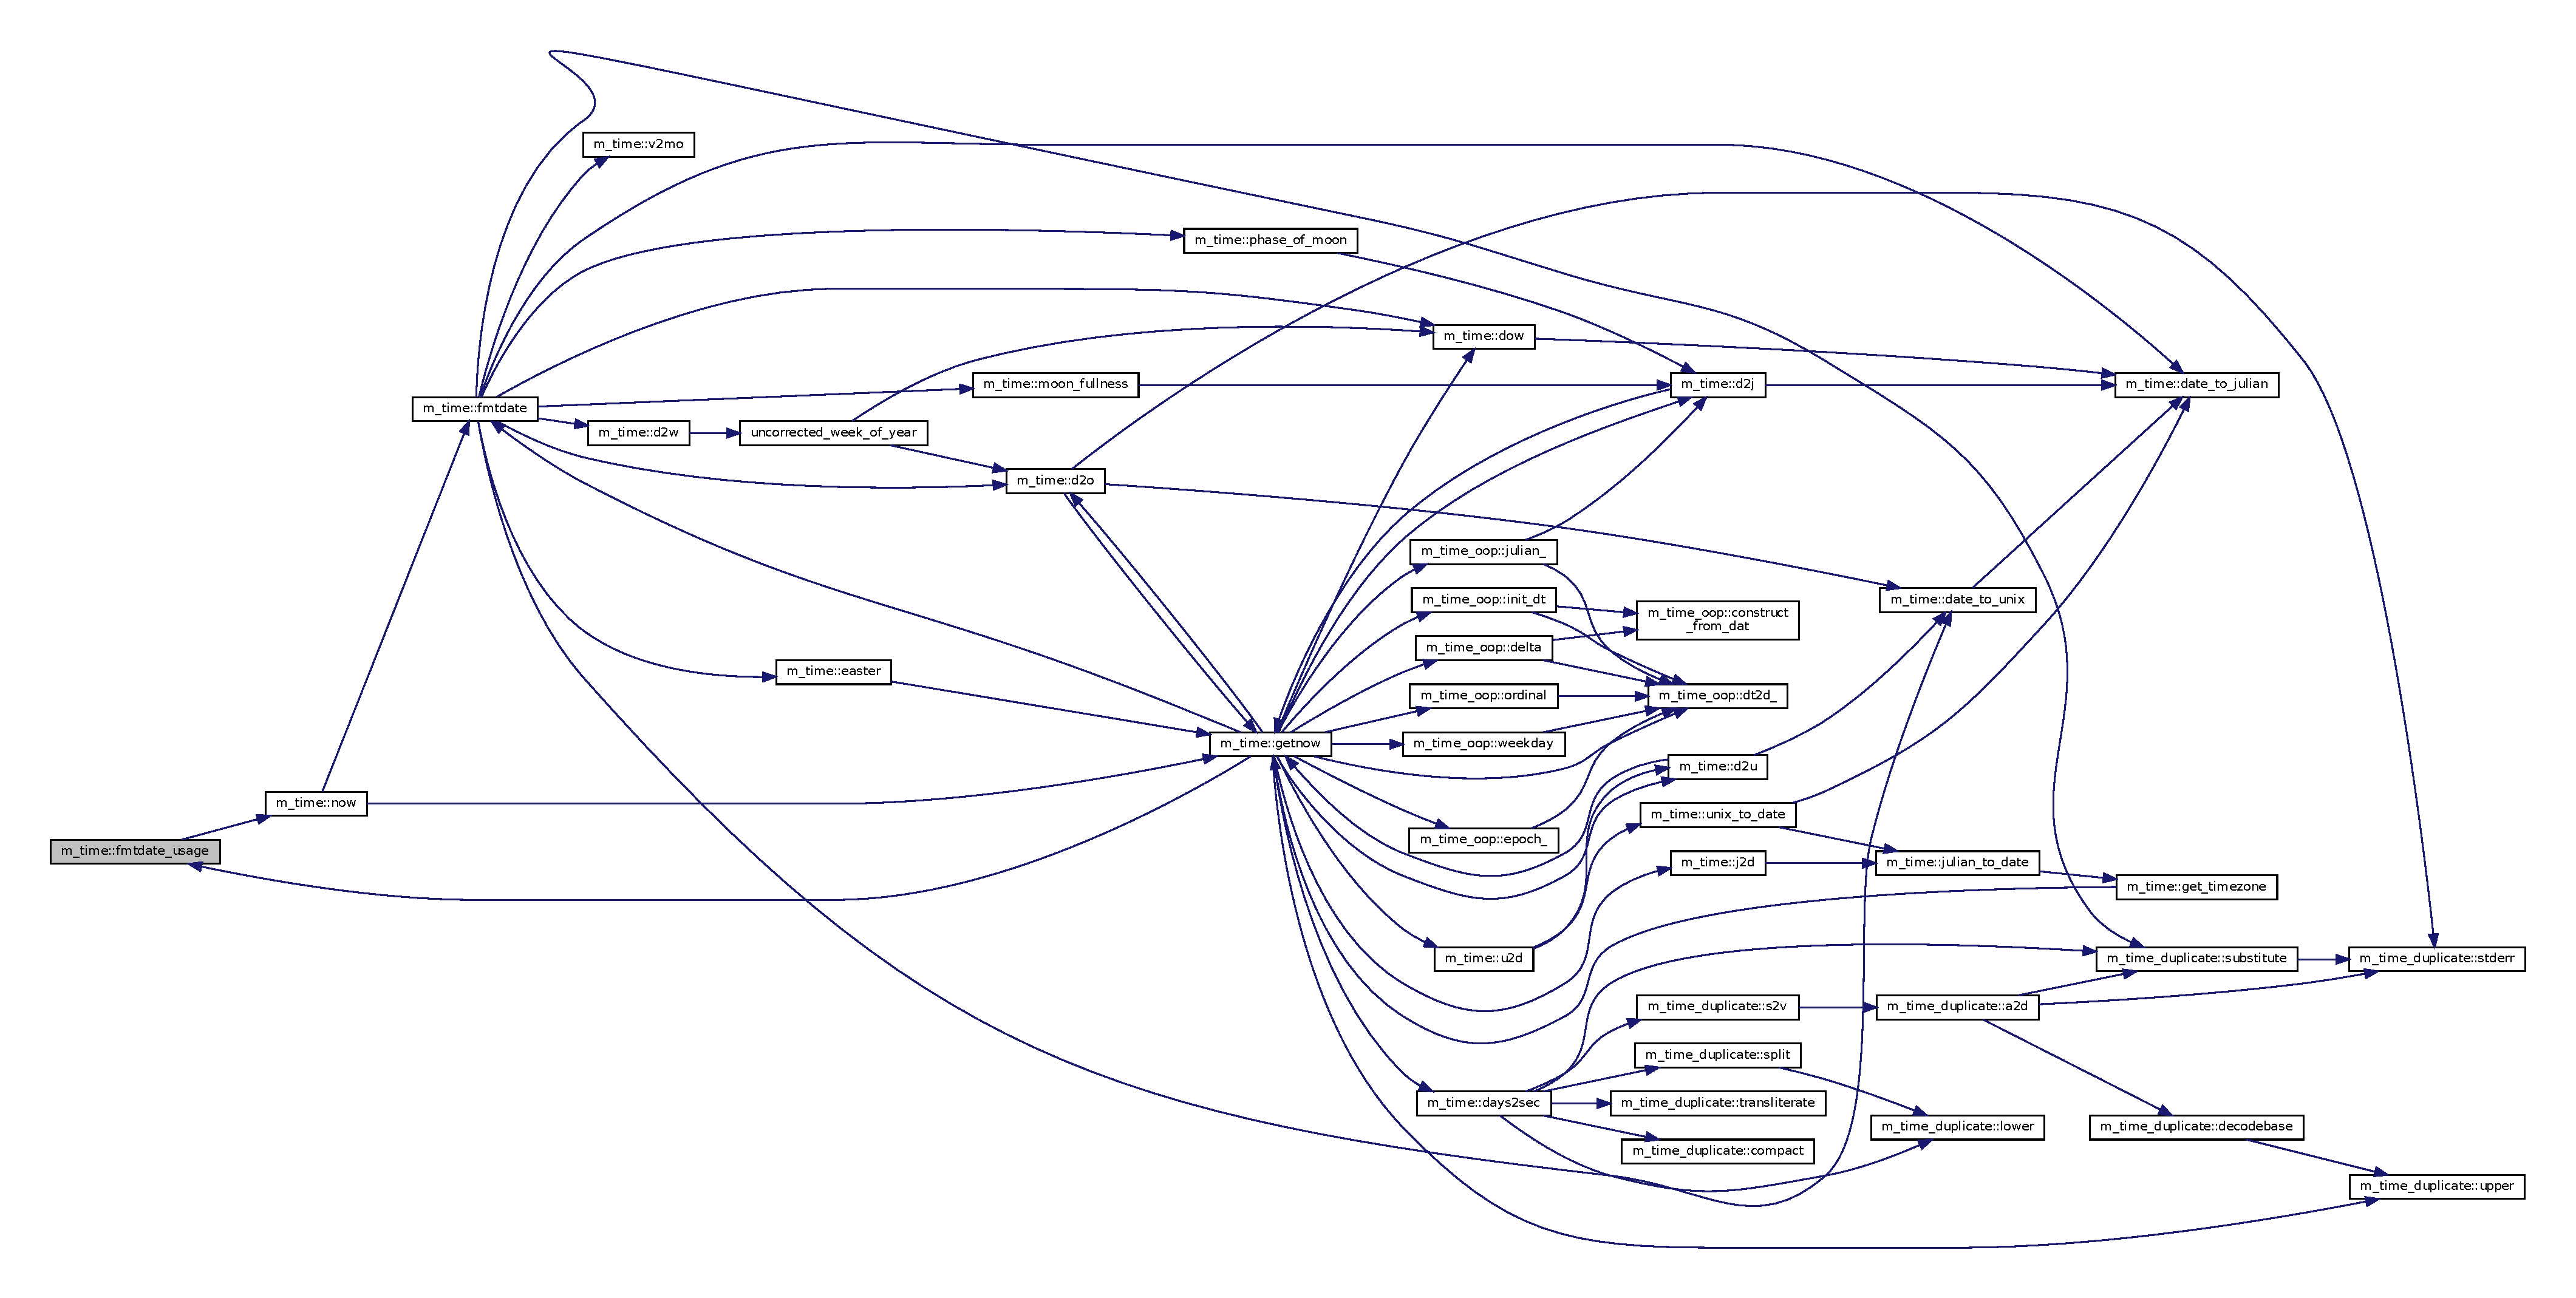
\includegraphics[width=350pt]{namespacem__time_a914927f70fb9495af1be2e484b967111_cgraph}
\end{center}
\end{figure}
\mbox{\Hypertarget{namespacem__time_a7903410a1d28bcdf3d33ab0c2d74b124}\label{namespacem__time_a7903410a1d28bcdf3d33ab0c2d74b124}} 
\index{m\_time@{m\_time}!get\_timezone@{get\_timezone}}
\index{get\_timezone@{get\_timezone}!m\_time@{m\_time}}
\doxysubsubsection{\texorpdfstring{get\_timezone()}{get\_timezone()}}
{\footnotesize\ttfamily integer function m\+\_\+time\+::get\+\_\+timezone\hspace{0.3cm}{\ttfamily [private]}}

Here is the caller graph for this function\+:\nopagebreak
\begin{figure}[H]
\begin{center}
\leavevmode
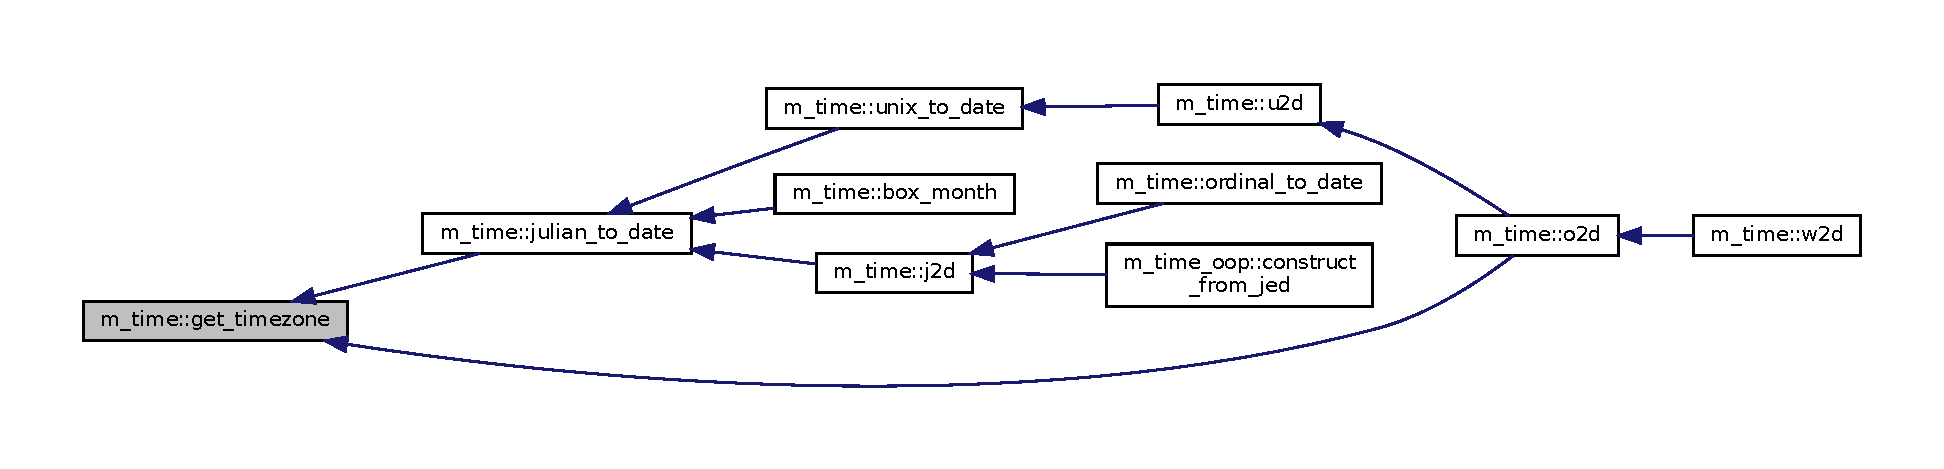
\includegraphics[width=350pt]{namespacem__time_a7903410a1d28bcdf3d33ab0c2d74b124_icgraph}
\end{center}
\end{figure}
\mbox{\Hypertarget{namespacem__time_aa5198c7aa4f3d8411c8ce93046ce3794}\label{namespacem__time_aa5198c7aa4f3d8411c8ce93046ce3794}} 
\index{m\_time@{m\_time}!guessdate@{guessdate}}
\index{guessdate@{guessdate}!m\_time@{m\_time}}
\doxysubsubsection{\texorpdfstring{guessdate()}{guessdate()}}
{\footnotesize\ttfamily subroutine, public m\+\_\+time\+::guessdate (\begin{DoxyParamCaption}\item[{character(len=$\ast$), intent(in)}]{datestring,  }\item[{integer, dimension(8), intent(out)}]{dat,  }\item[{integer, optional}]{ier }\end{DoxyParamCaption})}

\hypertarget{namespacem__time_autotoc_md109}{}\doxysubsubsection{N\+A\+ME}\label{namespacem__time_autotoc_md109}
guessdate(3f) -\/ \mbox{[}M\+\_\+time\+:R\+E\+A\+D\+I\+N\+G\+\_\+\+D\+A\+T\+ES\mbox{]} reads in a date, in various formats (L\+I\+C\+E\+N\+SE\+:PD)\hypertarget{namespacem__time_autotoc_md110}{}\doxysubsubsection{S\+Y\+N\+O\+P\+S\+IS}\label{namespacem__time_autotoc_md110}
\begin{DoxyVerb}subroutine guessdate(anot,dat)

 character(len=*),intent(in) :: anot
 integer,intent(out)         :: dat(8)
\end{DoxyVerb}
\hypertarget{namespacem__time_autotoc_md111}{}\doxysubsubsection{D\+E\+S\+C\+R\+I\+P\+T\+I\+ON}\label{namespacem__time_autotoc_md111}
Read in strings and except for looking for month names remove non-\/numeric characters and try to convert a string assumed to represent a date to a date-\/time array.

Years should always be expressed as four-\/digit numbers, and except for the special format yyyy-\/mm-\/dd the day should come after the year. Named months are preferred. If ambiguous the order is assumed to be day -\/ month -\/ year. Times are assumed to be of the form H\+H\+:\+MM\+:SS

It is planned that this routine will be superseded. As an alternative, a C routine exists in the standard C libraries that allows for expansive features when reading dates that can be called via the I\+S\+O\+\_\+\+C\+\_\+\+B\+I\+N\+D\+I\+NG interface.\hypertarget{namespacem__time_autotoc_md112}{}\doxysubsubsection{O\+P\+T\+I\+O\+NS}\label{namespacem__time_autotoc_md112}
anot A string assumed to represent a date including a year, month and day.

dat Integer array holding a \char`\"{}\+D\+A\+T\char`\"{} array, similar in structure to the array returned by the intrinsic D\+A\+T\+E\+\_\+\+A\+N\+D\+\_\+\+T\+I\+M\+E(3f)\+: \begin{DoxyVerb}   dat=[ year,month,day,timezone,hour,&
    & minutes,seconds,milliseconds]
\end{DoxyVerb}
\hypertarget{namespacem__time_autotoc_md113}{}\doxysubsubsection{E\+X\+A\+M\+P\+LE}\label{namespacem__time_autotoc_md113}
\begin{DoxyVerb}Sample program:

 program demo_guessdate
 use M_time, only : guessdate, fmtdate
 implicit none
 character(len=20),allocatable :: datestrings(:)
 character(len=:),allocatable  :: answer
 integer                       :: dat(8)
 integer                       :: i
    datestrings=[ &
    & 'January 9th, 2001   ',&
    & ' Tue Jul 19 2016    ',&
    & ' 21/12/2016         ',&
    & ' 4th of Jul 2004    ' ]
    do i=1,size(datestrings)
       write(*,'(a)')repeat('-',80)
       write(*,*)'TRYING ',datestrings(i)
       call guessdate(datestrings(i),dat)
       write(*,*)'DAT ARRAY ',dat
       answer=fmtdate(dat)
       write(*,*)'FOR '//datestrings(i)//' GOT '//trim(answer)
    enddo
 end program demo_guessdate

results:

 ---------------------------------------------------------------------
 TRYING January 9th, 2001
 DAT ARRAY         2001  1  9   -240    0   0   0    0
 FOR January 9th, 2001  GOT Tuesday, January 9th, 2001 12:00:00 AM
 ---------------------------------------------------------------------
 TRYING  Tue Jul 19 2016
 DAT ARRAY         2016  7  19  -240    0   0   0    0
 FOR  Tue Jul 19 2016   GOT Tuesday, July 19th, 2016 12:00:00 AM
 ---------------------------------------------------------------------
 TRYING  21/12/2016
 DAT ARRAY         2016  12 21  -240    0   0   0    0
 FOR  21/12/2016        GOT Wednesday, December 21st, 2016 12:00:00 AM
 ---------------------------------------------------------------------
 TRYING  4th of Jul 2004
 DAT ARRAY         2004  7  4   -240    0   0   0    0
 FOR  4th of Jul 2004   GOT Sunday, July 4th, 2004 12:00:00 AM
\end{DoxyVerb}
\hypertarget{namespacem__time_autotoc_md114}{}\doxysubsubsection{L\+I\+C\+E\+N\+SE}\label{namespacem__time_autotoc_md114}
Public Domain 

References m\+\_\+time\+\_\+duplicate\+::s2v(), m\+\_\+time\+\_\+duplicate\+::split(), m\+\_\+time\+\_\+duplicate\+::string\+\_\+to\+\_\+values(), m\+\_\+time\+\_\+duplicate\+::substitute(), and m\+\_\+time\+\_\+duplicate\+::upper().

Here is the call graph for this function\+:\nopagebreak
\begin{figure}[H]
\begin{center}
\leavevmode
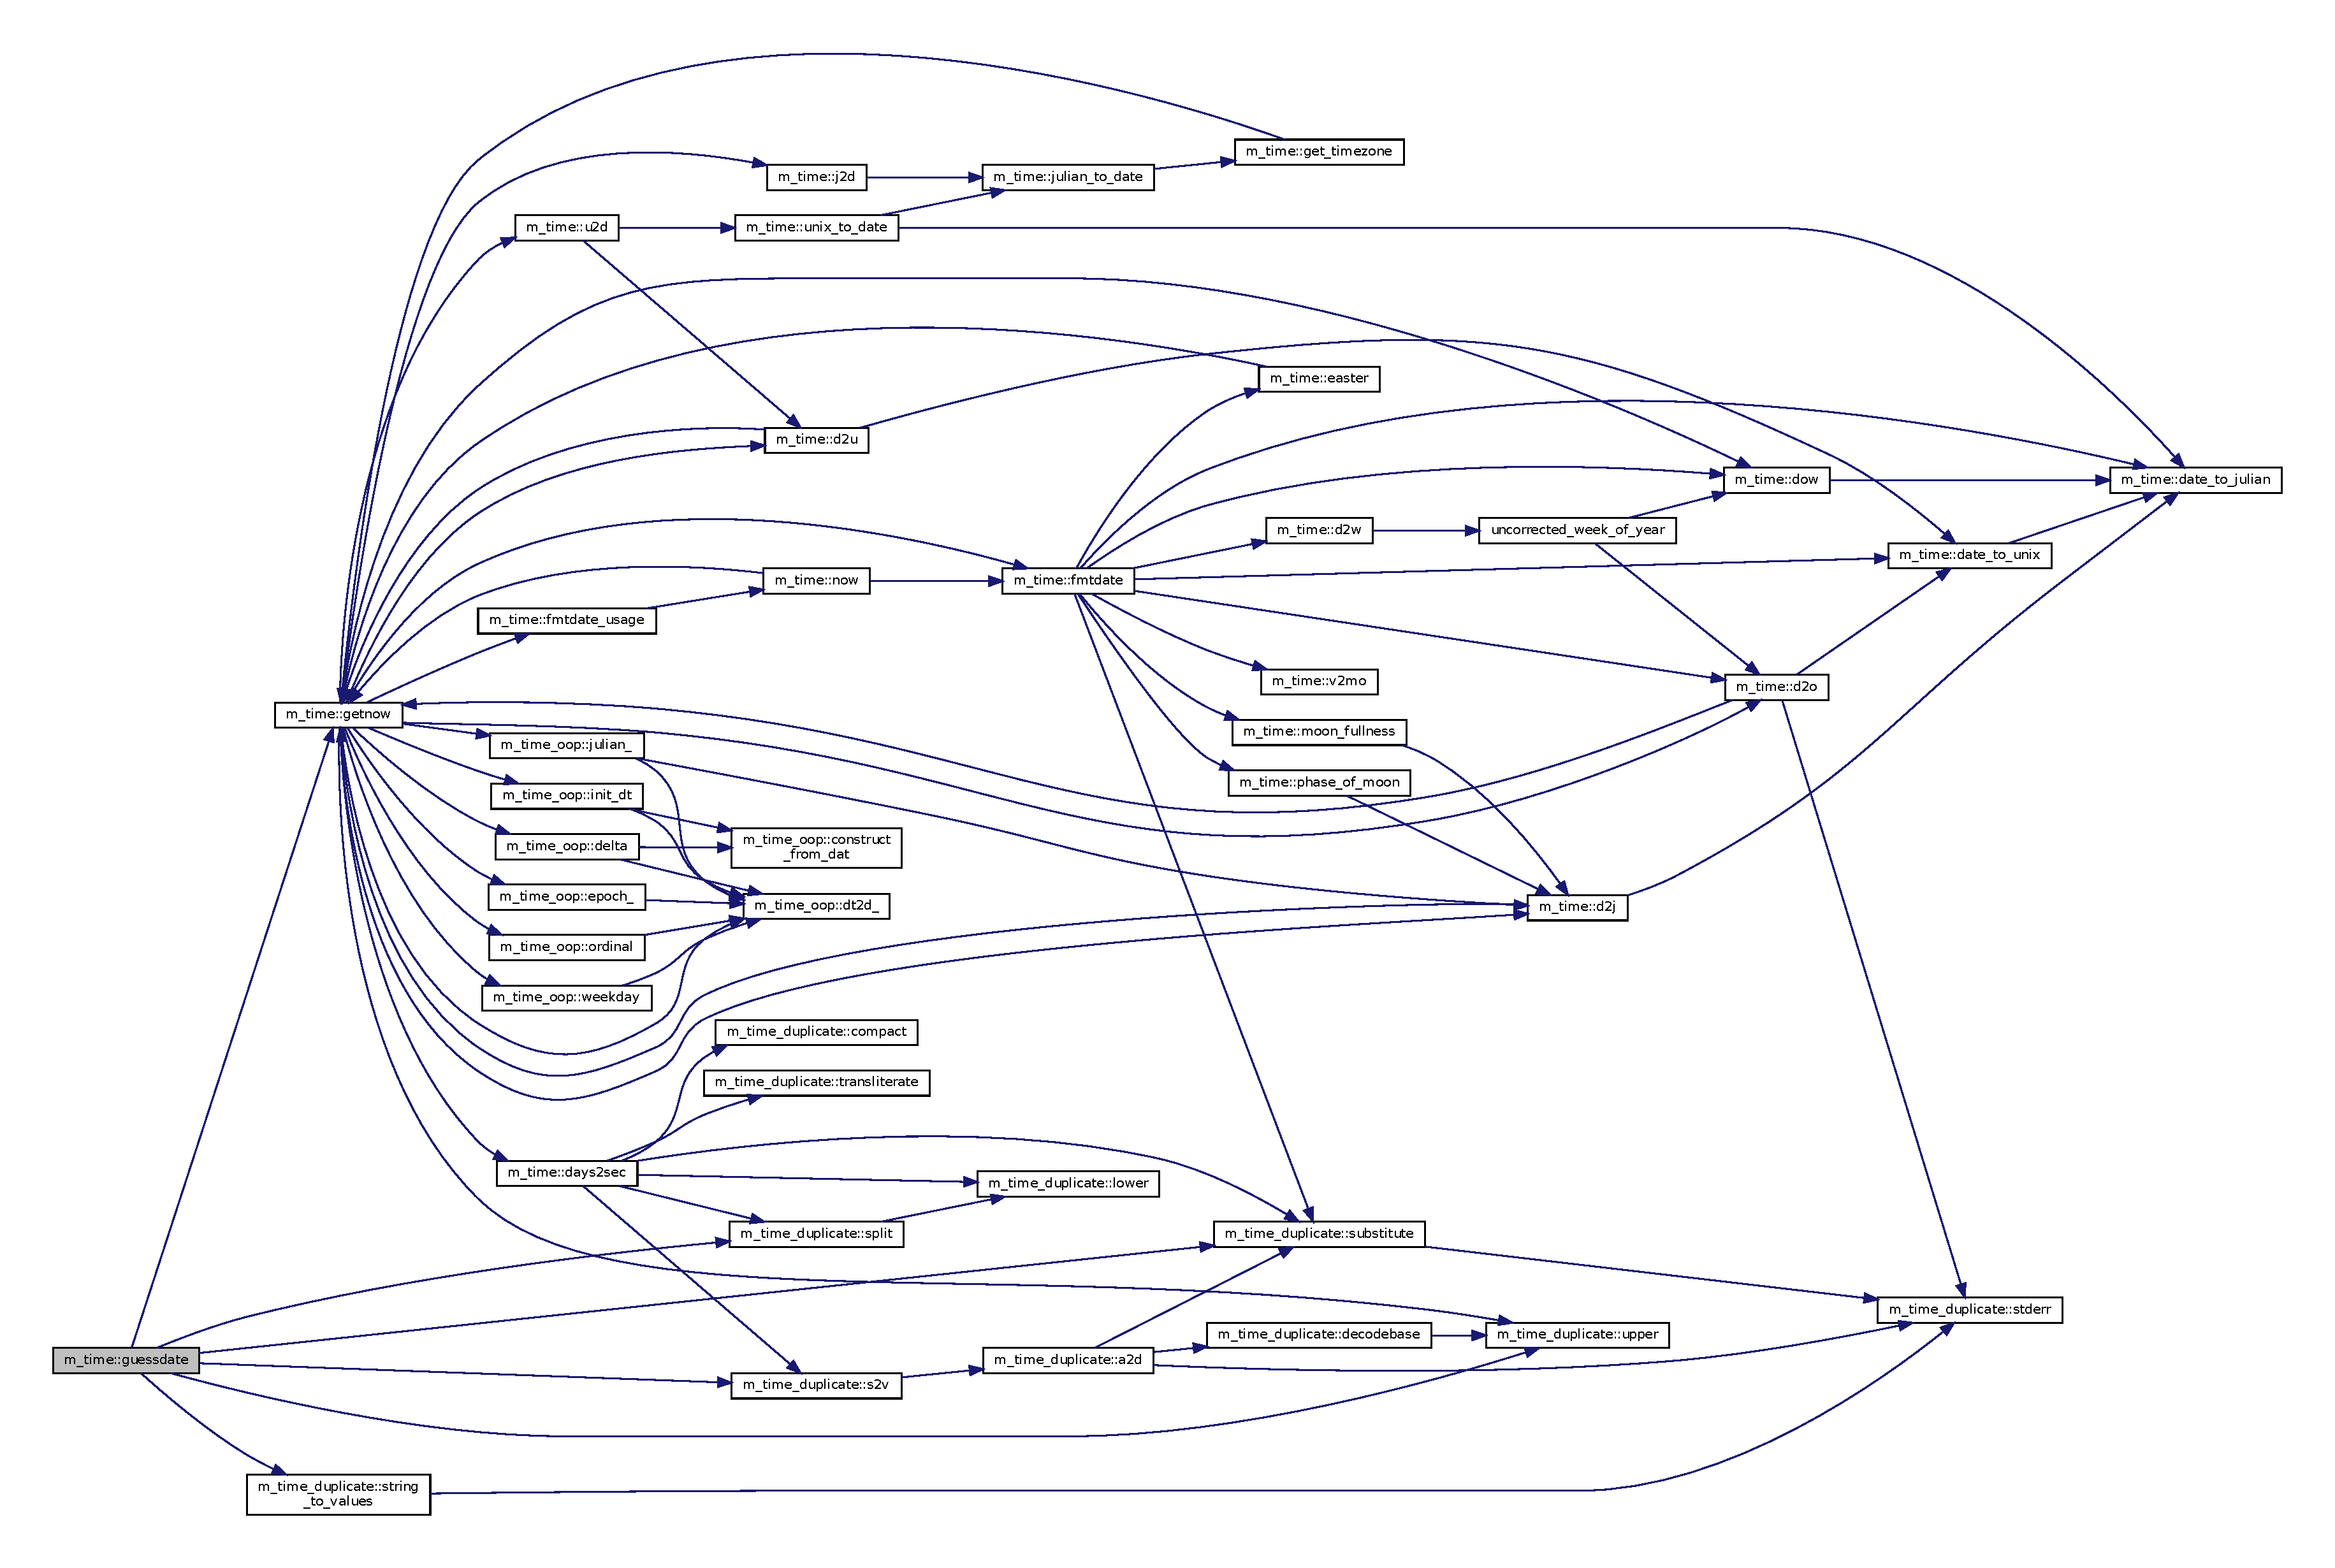
\includegraphics[width=350pt]{namespacem__time_aa5198c7aa4f3d8411c8ce93046ce3794_cgraph}
\end{center}
\end{figure}
\mbox{\Hypertarget{namespacem__time_a3ad5cad6df02c53e0429c3602a072e3c}\label{namespacem__time_a3ad5cad6df02c53e0429c3602a072e3c}} 
\index{m\_time@{m\_time}!j2d@{j2d}}
\index{j2d@{j2d}!m\_time@{m\_time}}
\doxysubsubsection{\texorpdfstring{j2d()}{j2d()}}
{\footnotesize\ttfamily integer function, dimension(8), public m\+\_\+time\+::j2d (\begin{DoxyParamCaption}\item[{real(kind=\mbox{\hyperlink{namespacem__time_ac10ea9e8d59ec74eaa7d89f2517d7422}{realtime}}), intent(in)}]{julian }\end{DoxyParamCaption})}

\hypertarget{namespacem__time_autotoc_md168}{}\doxysubsubsection{N\+A\+ME}\label{namespacem__time_autotoc_md168}
j2d(3f) -\/ \mbox{[}M\+\_\+time\+:J\+U\+L\+I\+AN\mbox{]} given a J\+ED (Julian Ephemeris Date) returns a date-\/time array D\+AT. (L\+I\+C\+E\+N\+SE\+:PD)\hypertarget{namespacem__time_autotoc_md169}{}\doxysubsubsection{S\+Y\+N\+O\+P\+S\+IS}\label{namespacem__time_autotoc_md169}
\begin{DoxyVerb}function j2d(julian) result (dat)

 real(kind=realtime),intent(in),optional :: julian
 integer                                 :: dat(8)
\end{DoxyVerb}
\hypertarget{namespacem__time_autotoc_md170}{}\doxysubsubsection{D\+E\+S\+C\+R\+I\+P\+T\+I\+ON}\label{namespacem__time_autotoc_md170}
Converts a Julian Ephemeris Date to a D\+AT date-\/time array.\hypertarget{namespacem__time_autotoc_md171}{}\doxysubsubsection{O\+P\+T\+I\+O\+NS}\label{namespacem__time_autotoc_md171}
julian A Julian Ephemeris Date (J\+ED) is the number of days since noon (not midnight) on January 1st, 4713 BC. If not present, use current time.\hypertarget{namespacem__time_autotoc_md172}{}\doxysubsubsection{R\+E\+T\+U\+R\+NS}\label{namespacem__time_autotoc_md172}
dat Integer array holding a \char`\"{}\+D\+A\+T\char`\"{} array, similar in structure to the array returned by the intrinsic D\+A\+T\+E\+\_\+\+A\+N\+D\+\_\+\+T\+I\+M\+E(3f)\+: \begin{DoxyVerb}   dat=[ year,month,day,timezone,hour,&
    & minutes,seconds,milliseconds]
\end{DoxyVerb}
\hypertarget{namespacem__time_autotoc_md173}{}\doxysubsubsection{E\+X\+A\+M\+P\+LE}\label{namespacem__time_autotoc_md173}
\begin{DoxyVerb}Sample program:

 program demo_j2d
 use M_time, only : j2d, d2j, fmtdate, realtime
 implicit none
 real(kind=realtime) :: today
 integer :: dat(8)
    call date_and_time(values=dat) ! get the date using intrinsic
    today=d2j(dat)                  ! convert today to Julian Date
    write(*,*)'Today=',fmtdate(j2d(today))
    ! math is easy with Julian Days and Julian Dates
    write(*,*)'Yesterday=',fmtdate(j2d(today-1.0d0))
    write(*,*)'Tomorrow=',fmtdate(j2d(today+1.0d0))
 end program demo_j2d

results:

 Today=Tuesday, July 19th, 2016 08:48:20 AM
 Yesterday=Monday, July 18th, 2016 08:48:20 AM
 Tomorrow=Wednesday, July 20th, 2016 08:48:20 AM
\end{DoxyVerb}
 \hypertarget{namespacem__time_autotoc_md174}{}\doxysubsubsection{A\+U\+T\+H\+OR}\label{namespacem__time_autotoc_md174}
John S. Urban, 2015 \hypertarget{namespacem__time_autotoc_md175}{}\doxysubsubsection{L\+I\+C\+E\+N\+SE}\label{namespacem__time_autotoc_md175}
Public Domain 

References julian\+\_\+to\+\_\+date().

Here is the call graph for this function\+:\nopagebreak
\begin{figure}[H]
\begin{center}
\leavevmode
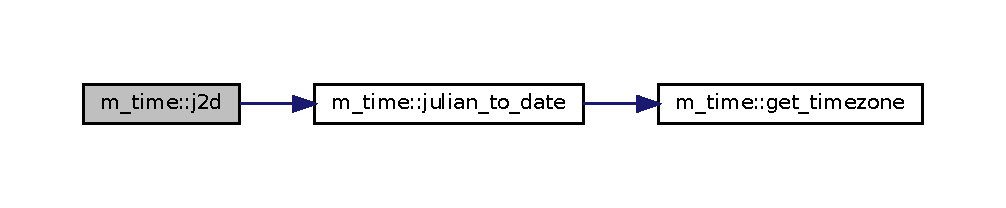
\includegraphics[width=350pt]{namespacem__time_a3ad5cad6df02c53e0429c3602a072e3c_cgraph}
\end{center}
\end{figure}
Here is the caller graph for this function\+:\nopagebreak
\begin{figure}[H]
\begin{center}
\leavevmode
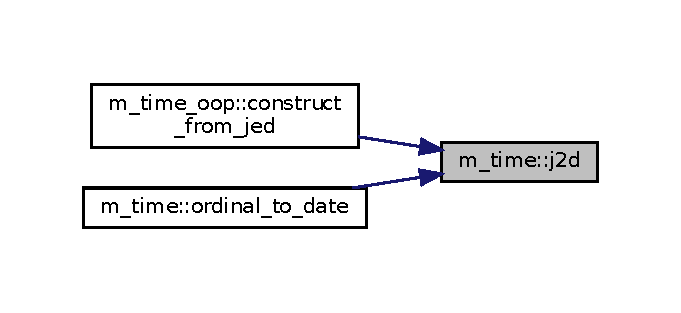
\includegraphics[width=327pt]{namespacem__time_a3ad5cad6df02c53e0429c3602a072e3c_icgraph}
\end{center}
\end{figure}
\mbox{\Hypertarget{namespacem__time_abb44cf18cd0a3e420c20469efb056203}\label{namespacem__time_abb44cf18cd0a3e420c20469efb056203}} 
\index{m\_time@{m\_time}!julian\_to\_date@{julian\_to\_date}}
\index{julian\_to\_date@{julian\_to\_date}!m\_time@{m\_time}}
\doxysubsubsection{\texorpdfstring{julian\_to\_date()}{julian\_to\_date()}}
{\footnotesize\ttfamily subroutine, public m\+\_\+time\+::julian\+\_\+to\+\_\+date (\begin{DoxyParamCaption}\item[{real(kind=\mbox{\hyperlink{namespacem__time_ac10ea9e8d59ec74eaa7d89f2517d7422}{realtime}}), intent(in)}]{julian,  }\item[{integer, dimension(8), intent(out)}]{dat,  }\item[{integer, intent(out)}]{ierr }\end{DoxyParamCaption})}

\hypertarget{namespacem__time_autotoc_md10}{}\doxysubsubsection{N\+A\+ME}\label{namespacem__time_autotoc_md10}
julian\+\_\+to\+\_\+date(3f) -\/ \mbox{[}M\+\_\+time\+:J\+U\+L\+I\+AN\mbox{]} converts a J\+ED(Julian Ephemeris Date) to a D\+AT date-\/time array. (L\+I\+C\+E\+N\+SE\+:PD)\hypertarget{namespacem__time_autotoc_md11}{}\doxysubsubsection{S\+Y\+N\+O\+P\+S\+IS}\label{namespacem__time_autotoc_md11}
\begin{DoxyVerb}subroutine julian_to_date(julian,dat,ierr)

 real(kind=realtime),intent(in) :: julian
 integer,intent(out)            :: dat(8)
 integer,intent(out)            :: ierr
\end{DoxyVerb}
\hypertarget{namespacem__time_autotoc_md12}{}\doxysubsubsection{D\+E\+S\+C\+R\+I\+P\+T\+I\+ON}\label{namespacem__time_autotoc_md12}
Converts a Unix Epoch Time (U\+ET) value to a D\+AT date-\/time array. U\+ET is the number of seconds since 00\+:00 on January 1st, 1970, U\+TC.\hypertarget{namespacem__time_autotoc_md13}{}\doxysubsubsection{O\+P\+T\+I\+O\+NS}\label{namespacem__time_autotoc_md13}
julian Julian Date (days) dat Integer array holding a \char`\"{}\+D\+A\+T\char`\"{} array, similar in structure to the array returned by the intrinsic D\+A\+T\+E\+\_\+\+A\+N\+D\+\_\+\+T\+I\+M\+E(3f)\+:

dat=\mbox{[} year,month,day,timezone,hour,\& \& minutes,seconds,milliseconds\mbox{]}\hypertarget{namespacem__time_autotoc_md14}{}\doxysubsubsection{R\+E\+T\+U\+R\+NS}\label{namespacem__time_autotoc_md14}
unixtime The \char`\"{}\+Unix Epoch\char`\"{} time, or the number of seconds since 00\+:00\+:00 on January 1st, 1970, U\+TC. ierr Error code. If 0 no error occurred.\hypertarget{namespacem__time_autotoc_md15}{}\doxysubsubsection{E\+X\+A\+M\+P\+LE}\label{namespacem__time_autotoc_md15}
\begin{DoxyVerb} Sample program:

  program demo_julian_to_date
  use M_time, only : julian_to_date, fmtdate, realtime
  implicit none
  real(kind=realtime)     :: juliandate
  integer                 :: dat(8)
  integer                 :: ierr
     ! set sample Julian Date
     juliandate=2457589.129d0
     ! create DAT array for this date
     call julian_to_date(juliandate,dat,ierr)
     write(*,*)'Sample Date=',fmtdate(dat)
     ! go back one day
     call julian_to_date(juliandate-1.0d0,dat,ierr)
     write(*,*)'Day Before =',fmtdate(dat)
     ! go forward one day
     call julian_to_date(juliandate+1.0d0,dat,ierr)
     write(*,*)'Day After  =',fmtdate(dat)
  end program demo_julian_to_date

 Results:

  Sample Date=Tuesday, July 19th, 2016 11:05:45 AM UTC-04:00
  Day Before =Monday, July 18th, 2016 11:05:45 AM UTC-04:00
  Day After  =Wednesday, July 20th, 2016 11:05:45 AM UTC-04:00
\end{DoxyVerb}
\hypertarget{namespacem__time_autotoc_md16}{}\doxysubsubsection{A\+U\+T\+H\+OR}\label{namespacem__time_autotoc_md16}
John S. Urban, 2015 \hypertarget{namespacem__time_autotoc_md17}{}\doxysubsubsection{L\+I\+C\+E\+N\+SE}\label{namespacem__time_autotoc_md17}
Public Domain 

References get\+\_\+timezone(), and secday.

Here is the call graph for this function\+:\nopagebreak
\begin{figure}[H]
\begin{center}
\leavevmode
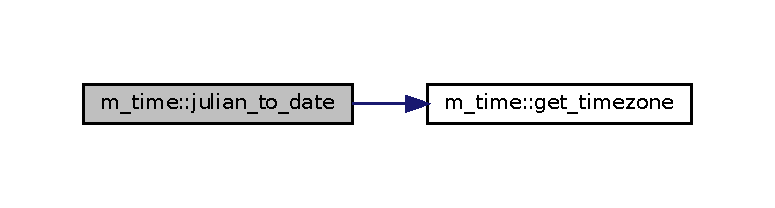
\includegraphics[width=350pt]{namespacem__time_abb44cf18cd0a3e420c20469efb056203_cgraph}
\end{center}
\end{figure}
Here is the caller graph for this function\+:\nopagebreak
\begin{figure}[H]
\begin{center}
\leavevmode
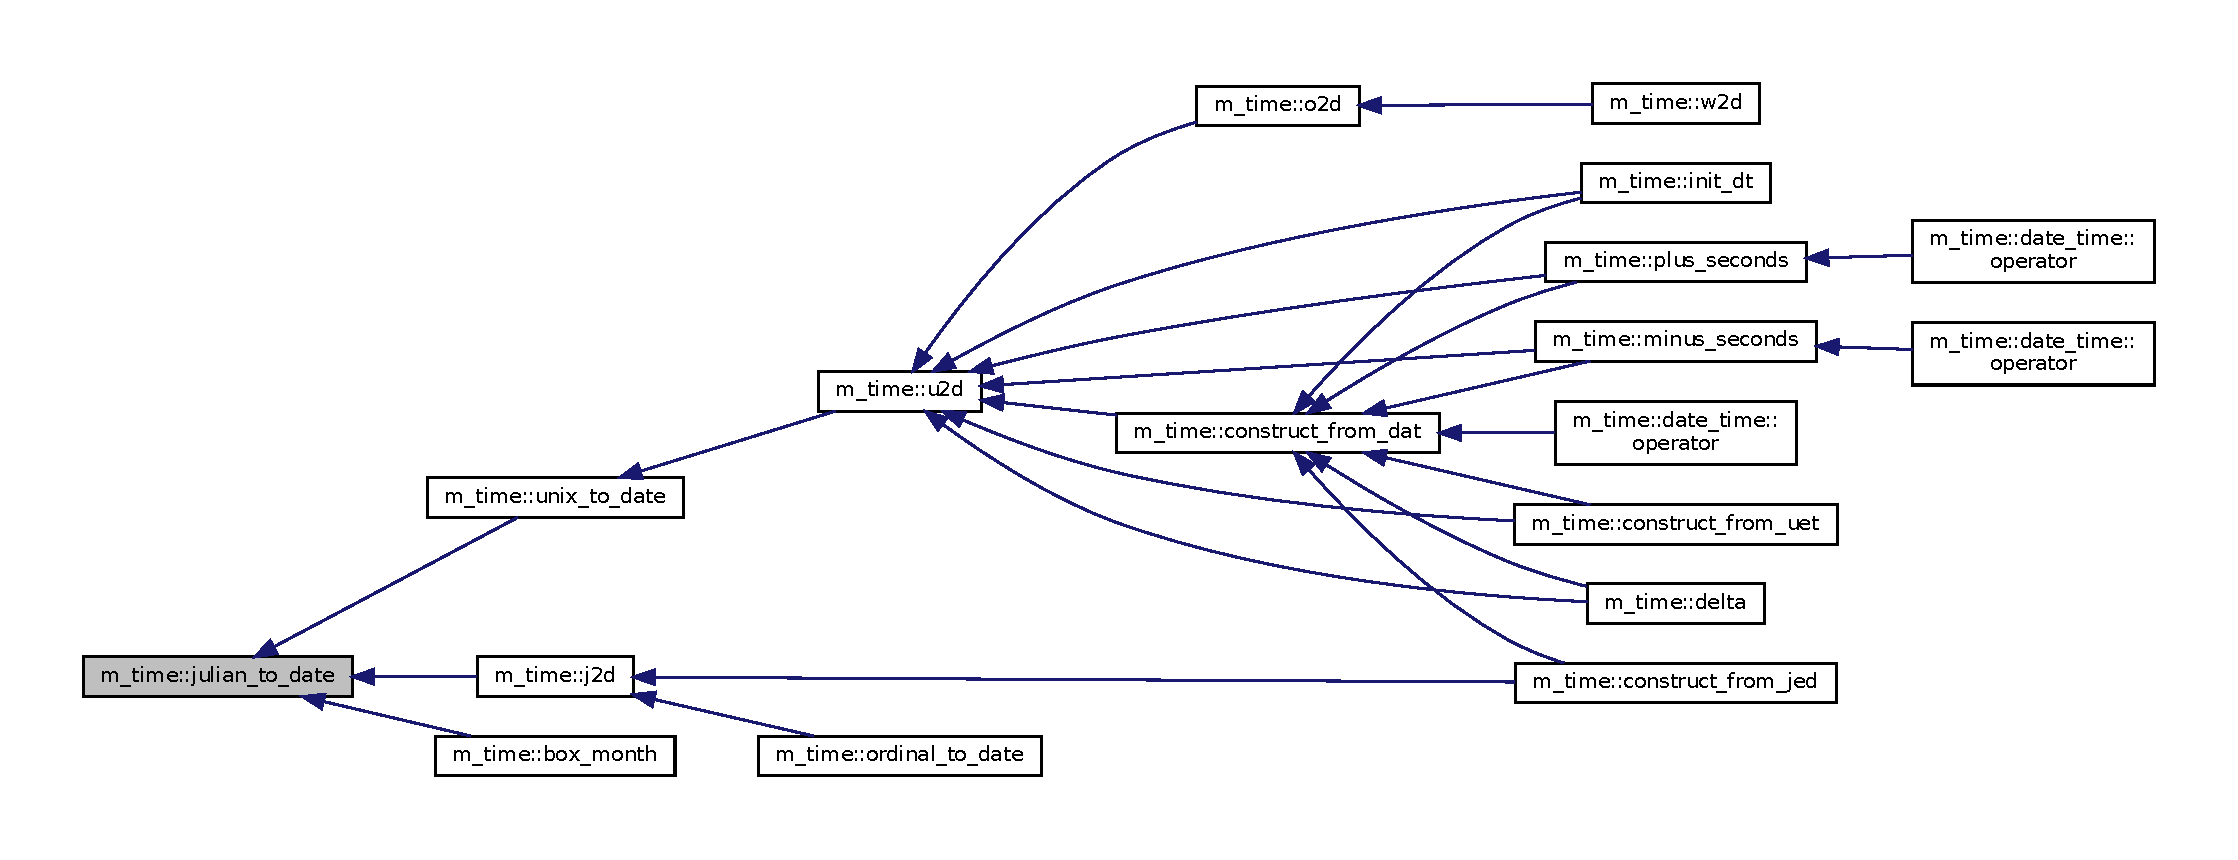
\includegraphics[width=350pt]{namespacem__time_abb44cf18cd0a3e420c20469efb056203_icgraph}
\end{center}
\end{figure}
\mbox{\Hypertarget{namespacem__time_a8188c7ed4e592c4f2388d28c75486726}\label{namespacem__time_a8188c7ed4e592c4f2388d28c75486726}} 
\index{m\_time@{m\_time}!mo2d@{mo2d}}
\index{mo2d@{mo2d}!m\_time@{m\_time}}
\doxysubsubsection{\texorpdfstring{mo2d()}{mo2d()}}
{\footnotesize\ttfamily integer function, dimension(8), public m\+\_\+time\+::mo2d (\begin{DoxyParamCaption}\item[{character(len=$\ast$), intent(in)}]{month\+\_\+name,  }\item[{integer, intent(in), optional}]{year }\end{DoxyParamCaption})}

\hypertarget{namespacem__time_autotoc_md70}{}\doxysubsubsection{N\+A\+ME}\label{namespacem__time_autotoc_md70}
mo2d(3f) -\/ \mbox{[}M\+\_\+time\+:M\+O\+N\+T\+H\+\_\+\+N\+A\+ME\mbox{]} given month name return D\+AT date-\/time array for beginning of that month in specified year (L\+I\+C\+E\+N\+SE\+:PD)\hypertarget{namespacem__time_autotoc_md71}{}\doxysubsubsection{S\+Y\+N\+O\+P\+S\+IS}\label{namespacem__time_autotoc_md71}
\begin{DoxyVerb}   function mo2d(month_name,year) result (dat)

    character(len=*),intent(in) :: month_name
    integer,intent(in),optional :: year
    integer                     :: dat(8)
\end{DoxyVerb}
\hypertarget{namespacem__time_autotoc_md72}{}\doxysubsubsection{D\+E\+S\+C\+R\+I\+P\+T\+I\+ON}\label{namespacem__time_autotoc_md72}
Given a Common Calendar month name, return the date as a \char`\"{}\+D\+A\+T\char`\"{} array for the 1st day of the month. An optional year may be specified. The year defaults to the current year.\hypertarget{namespacem__time_autotoc_md73}{}\doxysubsubsection{O\+P\+T\+I\+O\+NS}\label{namespacem__time_autotoc_md73}
month\+\_\+name A string representing a Common Calendar month name. year Optional year. Defaults to current year \hypertarget{namespacem__time_autotoc_md74}{}\doxysubsubsection{R\+E\+T\+U\+R\+NS}\label{namespacem__time_autotoc_md74}
dat An integer array that has the same structure as the array returned by the Fortran intrinsic D\+A\+T\+E\+\_\+\+A\+N\+D\+\_\+\+T\+I\+M\+E(3f)\+:

dat=\mbox{[} year,month,day,timezone,hour,\& \& minutes,seconds,milliseconds\mbox{]}\hypertarget{namespacem__time_autotoc_md75}{}\doxysubsubsection{E\+X\+A\+M\+P\+LE}\label{namespacem__time_autotoc_md75}
\begin{DoxyVerb}Sample program:

 program demo_mo2d
 use M_time, only : mo2d
 implicit none
    write(*,'(*(i0:,":"))')mo2d('March')
 end program demo_mo2d

results:

   2016:3:1:-240:0:0:0:0
\end{DoxyVerb}
\hypertarget{namespacem__time_autotoc_md76}{}\doxysubsubsection{A\+U\+T\+H\+OR}\label{namespacem__time_autotoc_md76}
John S. Urban, 2015 \hypertarget{namespacem__time_autotoc_md77}{}\doxysubsubsection{L\+I\+C\+E\+N\+SE}\label{namespacem__time_autotoc_md77}
Public Domain 

References mo2v(), and m\+\_\+time\+\_\+duplicate\+::stderr().

Here is the call graph for this function\+:\nopagebreak
\begin{figure}[H]
\begin{center}
\leavevmode
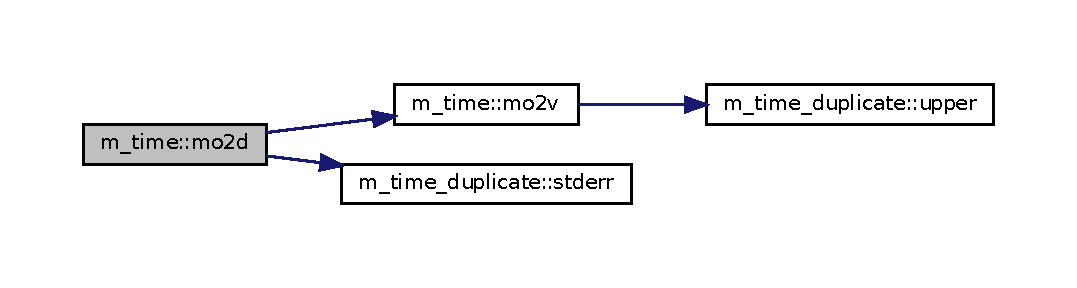
\includegraphics[width=350pt]{namespacem__time_a8188c7ed4e592c4f2388d28c75486726_cgraph}
\end{center}
\end{figure}
\mbox{\Hypertarget{namespacem__time_ad7bf0886754757e8961e562f06cf3bb7}\label{namespacem__time_ad7bf0886754757e8961e562f06cf3bb7}} 
\index{m\_time@{m\_time}!mo2v@{mo2v}}
\index{mo2v@{mo2v}!m\_time@{m\_time}}
\doxysubsubsection{\texorpdfstring{mo2v()}{mo2v()}}
{\footnotesize\ttfamily integer function, public m\+\_\+time\+::mo2v (\begin{DoxyParamCaption}\item[{character(len=$\ast$), intent(in)}]{month\+\_\+name }\end{DoxyParamCaption})}

\hypertarget{namespacem__time_autotoc_md78}{}\doxysubsubsection{N\+A\+ME}\label{namespacem__time_autotoc_md78}
mo2v(3f) -\/ \mbox{[}M\+\_\+time\+:M\+O\+N\+T\+H\+\_\+\+N\+A\+ME\mbox{]} given month name return month number (1-\/12) of that month (L\+I\+C\+E\+N\+SE\+:PD)\hypertarget{namespacem__time_autotoc_md79}{}\doxysubsubsection{S\+Y\+N\+O\+P\+S\+IS}\label{namespacem__time_autotoc_md79}
\begin{DoxyVerb}function mo2v(month_name) result(imonth)

  character(len=*),intent(in):: month_name ! month name
  integer                    :: imonth     ! month number
\end{DoxyVerb}
\hypertarget{namespacem__time_autotoc_md80}{}\doxysubsubsection{D\+E\+S\+C\+R\+I\+P\+T\+I\+ON}\label{namespacem__time_autotoc_md80}
Given a string representing the name or abbreviation of a Gregorian Calendar month return a number representing the position of the month in the calendar starting with 1 for January and ending with 12 for December.\hypertarget{namespacem__time_autotoc_md81}{}\doxysubsubsection{O\+P\+T\+I\+O\+NS}\label{namespacem__time_autotoc_md81}
month\+\_\+name name or abbreviation of month. Case is ignored Once enough characters are found to uniquely identify a month the rest of the name is ignored. \hypertarget{namespacem__time_autotoc_md82}{}\doxysubsubsection{R\+E\+T\+U\+R\+NS}\label{namespacem__time_autotoc_md82}
imonth month number returned. If the name is not recognized a -\/1 is returned.\hypertarget{namespacem__time_autotoc_md83}{}\doxysubsubsection{E\+X\+A\+M\+P\+LE}\label{namespacem__time_autotoc_md83}
\begin{DoxyVerb}Sample program:

 program demo_mo2v
 use M_time, only : mo2v
 implicit none
    write(*,*)mo2v("April")
    write(*,*)mo2v('Apr')
    ! NOTE: still matches September, as "SE" was enough
    write(*,*)mo2v('sexember')
    write(*,*)mo2v('unknown')  ! returns -1
 end program demo_mo2v

results:

   >  4
   >  4
   >  9
   > -1
\end{DoxyVerb}
\hypertarget{namespacem__time_autotoc_md84}{}\doxysubsubsection{A\+U\+T\+H\+OR}\label{namespacem__time_autotoc_md84}
John S. Urban, 2015 \hypertarget{namespacem__time_autotoc_md85}{}\doxysubsubsection{L\+I\+C\+E\+N\+SE}\label{namespacem__time_autotoc_md85}
Public Domain 

References m\+\_\+time\+\_\+duplicate\+::upper().

Here is the call graph for this function\+:\nopagebreak
\begin{figure}[H]
\begin{center}
\leavevmode
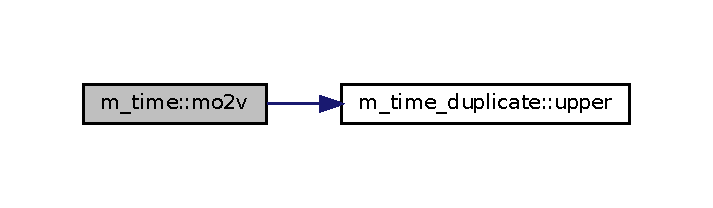
\includegraphics[width=342pt]{namespacem__time_ad7bf0886754757e8961e562f06cf3bb7_cgraph}
\end{center}
\end{figure}
Here is the caller graph for this function\+:\nopagebreak
\begin{figure}[H]
\begin{center}
\leavevmode
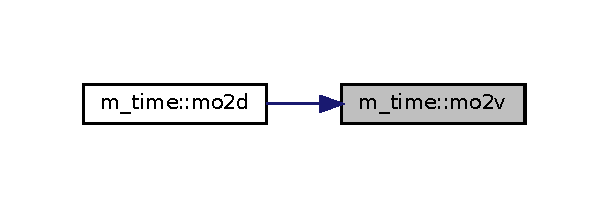
\includegraphics[width=292pt]{namespacem__time_ad7bf0886754757e8961e562f06cf3bb7_icgraph}
\end{center}
\end{figure}
\mbox{\Hypertarget{namespacem__time_a702b39998a769b8f60070c0bec975ee2}\label{namespacem__time_a702b39998a769b8f60070c0bec975ee2}} 
\index{m\_time@{m\_time}!moon\_fullness@{moon\_fullness}}
\index{moon\_fullness@{moon\_fullness}!m\_time@{m\_time}}
\doxysubsubsection{\texorpdfstring{moon\_fullness()}{moon\_fullness()}}
{\footnotesize\ttfamily integer function, public m\+\_\+time\+::moon\+\_\+fullness (\begin{DoxyParamCaption}\item[{integer, dimension(8), intent(in)}]{datin }\end{DoxyParamCaption})}

\hypertarget{namespacem__time_autotoc_md214}{}\doxysubsubsection{N\+A\+ME}\label{namespacem__time_autotoc_md214}
moon\+\_\+fullness(3f) -\/ \mbox{[}M\+\_\+time\+:A\+S\+T\+R\+O\+L\+O\+G\+I\+C\+AL\mbox{]} return percentage of moon phase from new to full (L\+I\+C\+E\+N\+SE\+:PD) \hypertarget{namespacem__time_autotoc_md215}{}\doxysubsubsection{S\+Y\+N\+O\+P\+S\+IS}\label{namespacem__time_autotoc_md215}
function moon\+\_\+fullness(datin)

integer,intent(in) \+:: datin(8) integer \+:: moon\+\_\+fullness\hypertarget{namespacem__time_autotoc_md216}{}\doxysubsubsection{D\+E\+S\+C\+R\+I\+P\+T\+I\+ON}\label{namespacem__time_autotoc_md216}
This procedure is used to support the P field descriptor for the fmtdate(3f) routine.

The moon circles the earth every 29.\+530588853 days on average, so pick a starting point and count. A new moon occurred at January 6, 2000, 18\+:14 U\+TC. Then it is easy to count the number of days since the last new moon. This is an approximate calculation.\hypertarget{namespacem__time_autotoc_md217}{}\doxysubsubsection{O\+P\+T\+I\+O\+NS}\label{namespacem__time_autotoc_md217}
datin D\+AT Date array describing input date\hypertarget{namespacem__time_autotoc_md218}{}\doxysubsubsection{R\+E\+S\+U\+L\+TS}\label{namespacem__time_autotoc_md218}
\begin{DoxyVerb} moon_fullness  0 is a new or dark moon, 100 is a full moon, + for waxing
                and - for waning.
\end{DoxyVerb}
\hypertarget{namespacem__time_autotoc_md219}{}\doxysubsubsection{E\+X\+A\+M\+P\+L\+ES}\label{namespacem__time_autotoc_md219}
\begin{DoxyVerb}Sample:

 program demo_moon_fullness
 use M_time, only : now
 use M_time, only : phase_of_moon
 use M_time, only : moon_fullness
 implicit none
 integer             :: dat(8)
    ! generate DAT array
    call date_and_time(values=dat)
    ! show DAT array
    write(*,'(" Today is:",*(i0:,":"))')dat
    ! the %p and %P fields are supported by fmtdate(3f)
    write(*,*)&
    &now('The phase of the moon is %p, with a fullness of %P')
    write(*,'(1x,*(a))',advance='no')&
    &'The phase of the moon is ',trim( phase_of_moon(dat)),','
    write(*,'(1x,a,i0,a)')&
    &'with a fullness of ', moon_fullness(dat),'%'
 end program demo_moon_fullness

Sample output:

  Today is:2018:11:3:-240:20:18:44:245
  The phase of the moon is Waning crescent, with a fullness of -30%
  The phase of the moon is Waning crescent, with a fullness of -30%
\end{DoxyVerb}
 \hypertarget{namespacem__time_autotoc_md220}{}\doxysubsubsection{A\+U\+T\+H\+OR}\label{namespacem__time_autotoc_md220}
John S. Urban, 2015 \hypertarget{namespacem__time_autotoc_md221}{}\doxysubsubsection{L\+I\+C\+E\+N\+SE}\label{namespacem__time_autotoc_md221}
Public Domain 

References d2j().

Here is the call graph for this function\+:\nopagebreak
\begin{figure}[H]
\begin{center}
\leavevmode
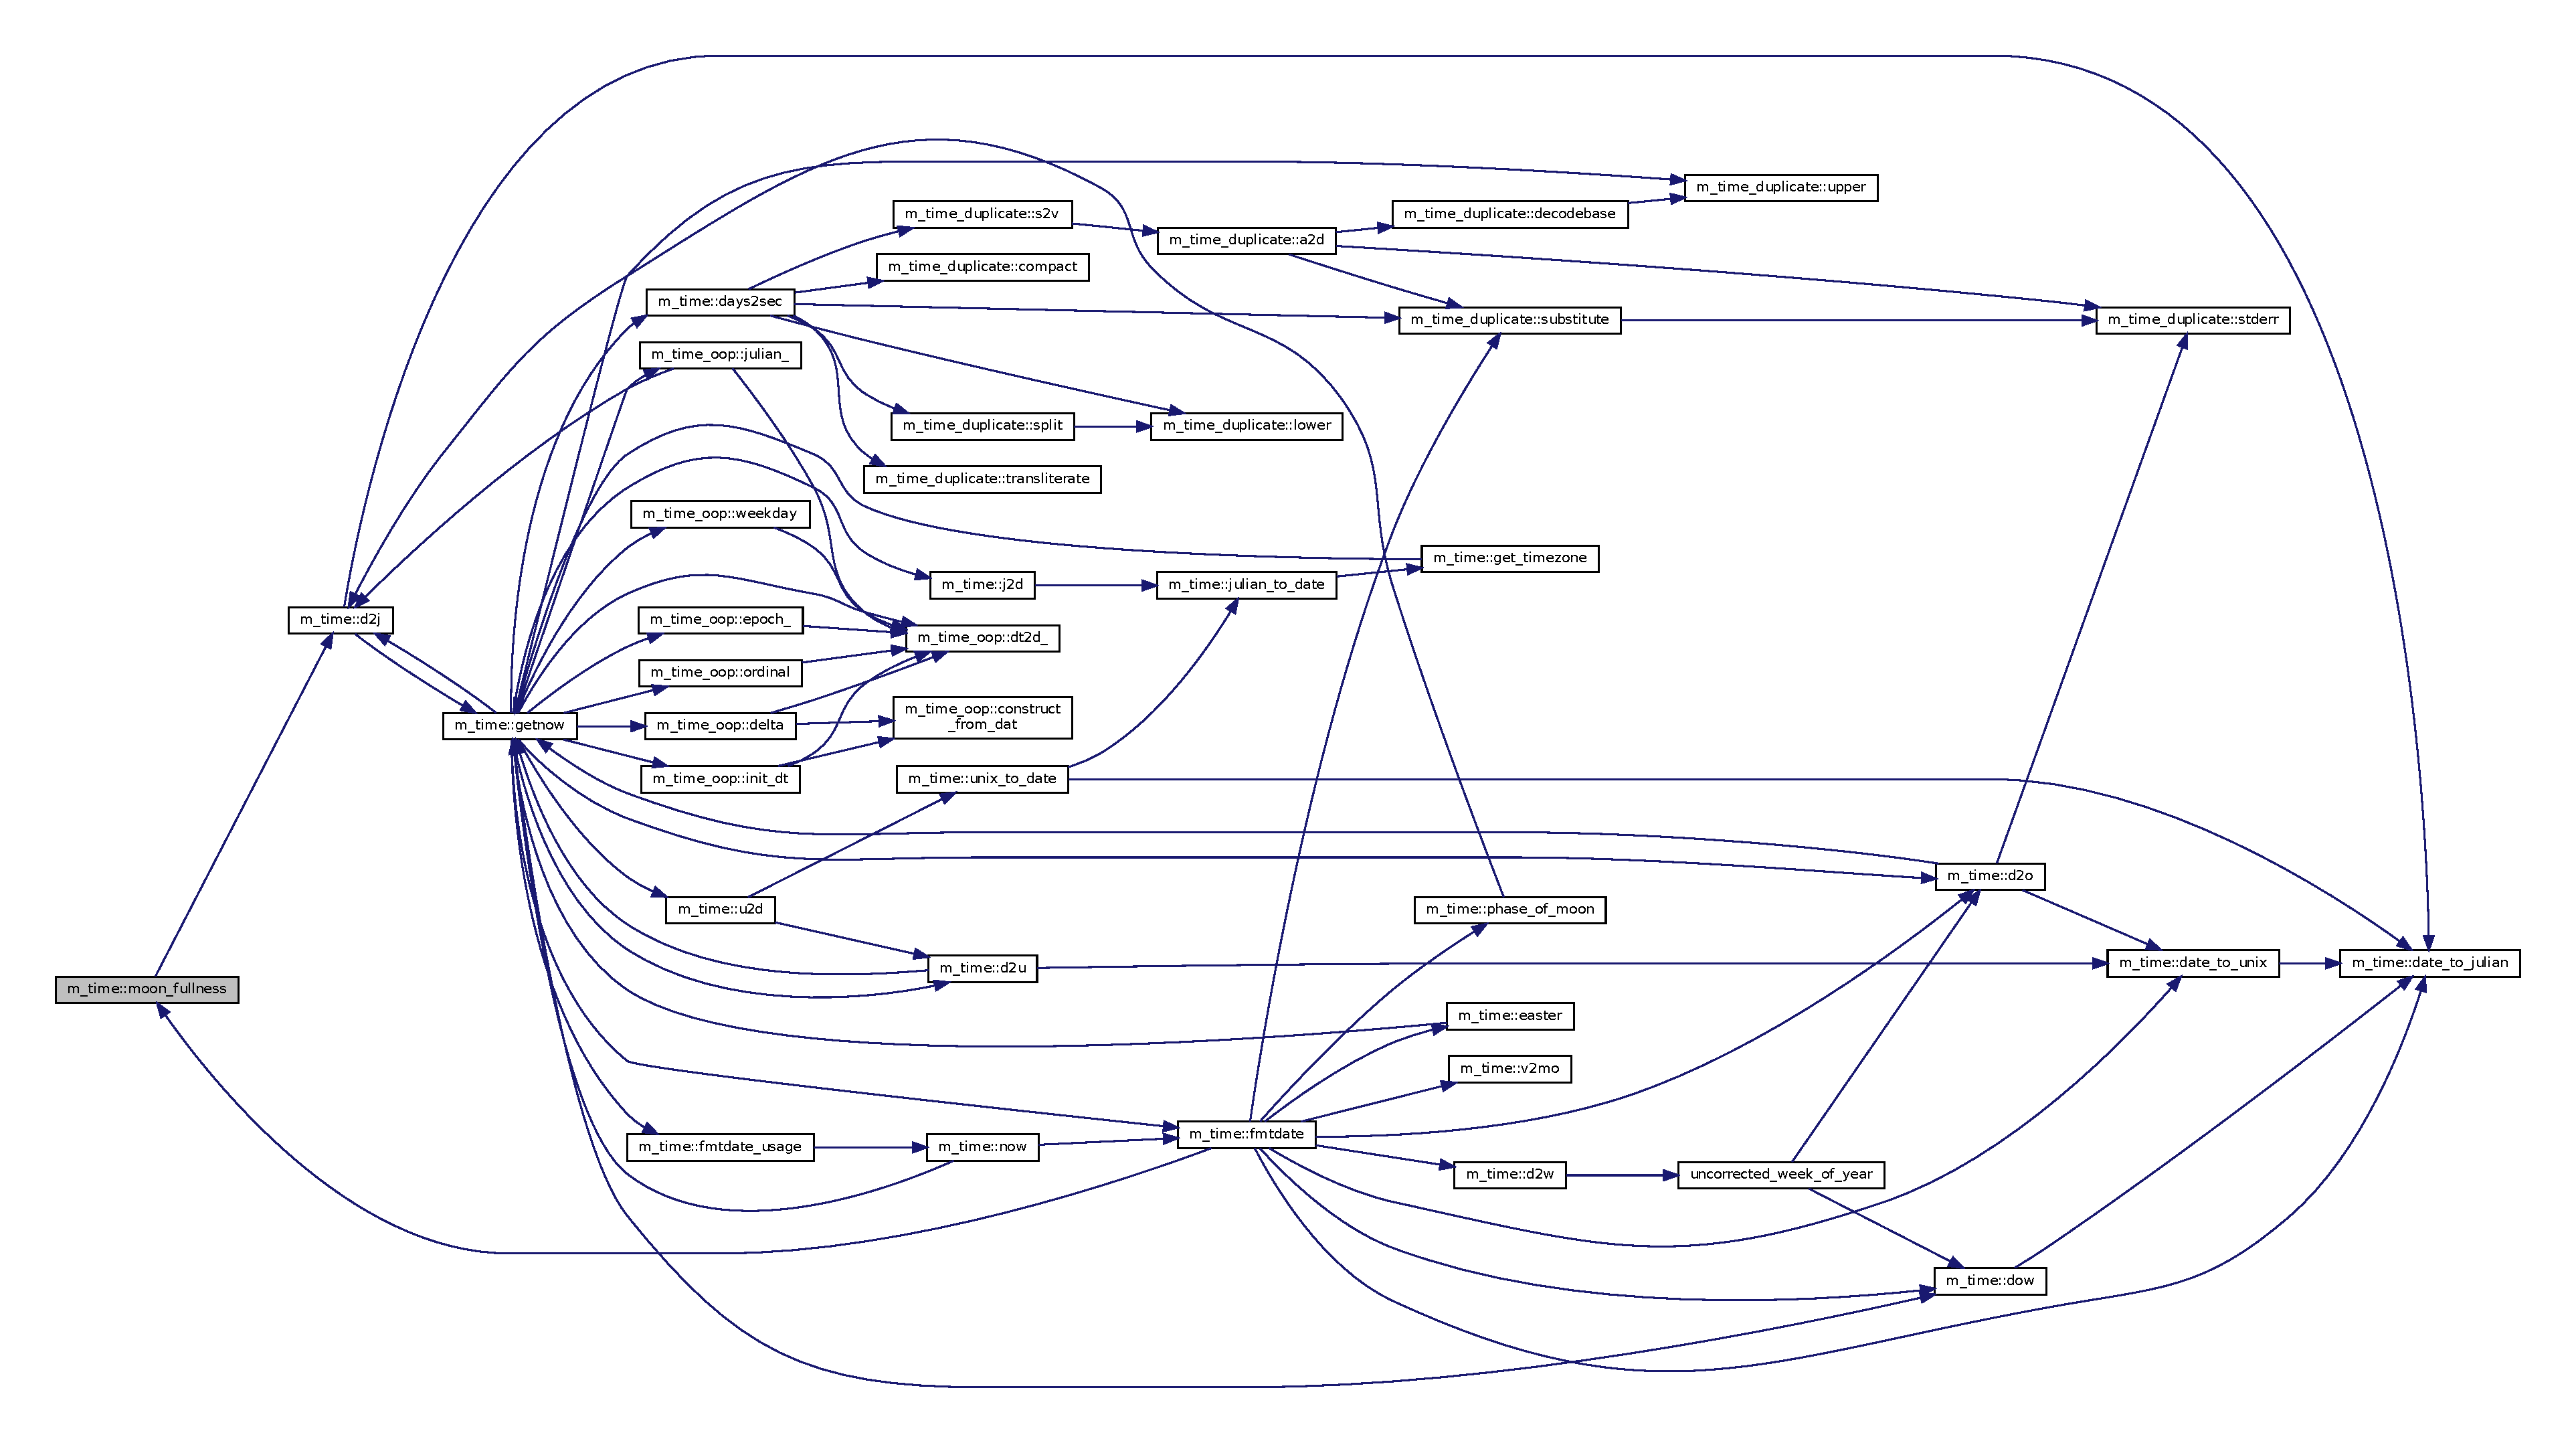
\includegraphics[width=350pt]{namespacem__time_a702b39998a769b8f60070c0bec975ee2_cgraph}
\end{center}
\end{figure}
Here is the caller graph for this function\+:\nopagebreak
\begin{figure}[H]
\begin{center}
\leavevmode
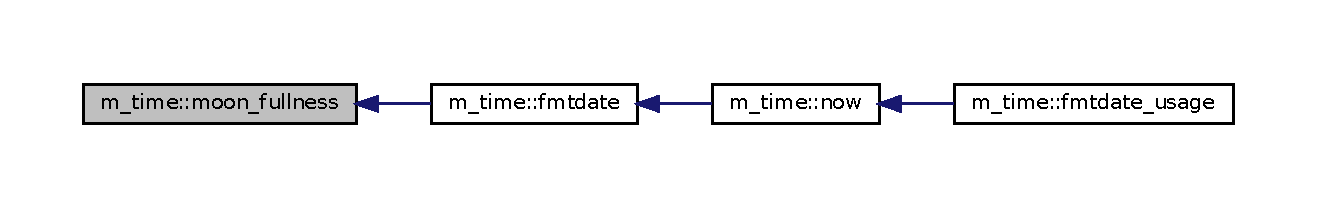
\includegraphics[width=350pt]{namespacem__time_a702b39998a769b8f60070c0bec975ee2_icgraph}
\end{center}
\end{figure}
\mbox{\Hypertarget{namespacem__time_a6b5e87be0e510ff268c1ecfbf67a3bdb}\label{namespacem__time_a6b5e87be0e510ff268c1ecfbf67a3bdb}} 
\index{m\_time@{m\_time}!now@{now}}
\index{now@{now}!m\_time@{m\_time}}
\doxysubsubsection{\texorpdfstring{now()}{now()}}
{\footnotesize\ttfamily character(len=\+:) function, allocatable, public m\+\_\+time\+::now (\begin{DoxyParamCaption}\item[{character(len=$\ast$), intent(in), optional}]{format }\end{DoxyParamCaption})}

\hypertarget{namespacem__time_autotoc_md86}{}\doxysubsubsection{N\+A\+ME}\label{namespacem__time_autotoc_md86}
now(3f) -\/ \mbox{[}M\+\_\+time\+:D\+A\+T\+E\+\_\+\+P\+R\+I\+N\+T\+I\+NG\mbox{]} return string representing current time given format (L\+I\+C\+E\+N\+SE\+:PD)\hypertarget{namespacem__time_autotoc_md87}{}\doxysubsubsection{S\+Y\+N\+O\+P\+S\+IS}\label{namespacem__time_autotoc_md87}
\begin{DoxyVerb}function now(format) RESULT (timestr)

 character(len=*),intent(in)     :: format  ! input format string
 character(len=:),allocatable    :: timestr ! formatted date
\end{DoxyVerb}
\hypertarget{namespacem__time_autotoc_md88}{}\doxysubsubsection{D\+E\+S\+C\+R\+I\+P\+T\+I\+ON}\label{namespacem__time_autotoc_md88}
The now(3f) function is a call to the fmtdate(3f) function using the current date and time. That is, it is a convenient way to print the current date and time.\hypertarget{namespacem__time_autotoc_md89}{}\doxysubsubsection{O\+P\+T\+I\+O\+NS}\label{namespacem__time_autotoc_md89}
format string describing how to format the current date and time. For a complete description of the formatting macros supported see fmtdate\+\_\+usage(3f). \hypertarget{namespacem__time_autotoc_md90}{}\doxysubsubsection{R\+E\+T\+U\+R\+NS}\label{namespacem__time_autotoc_md90}
timestr formatted output string representing date\hypertarget{namespacem__time_autotoc_md91}{}\doxysubsubsection{E\+X\+A\+M\+P\+LE}\label{namespacem__time_autotoc_md91}
\begin{DoxyVerb}Sample Program:

 program demo_now
 use M_time, only : now
 implicit none
    write(*,*)now("The current date is %w, %l %d, %Y %H:%m:%s %N")
    call showme()
 contains
 subroutine showme() ! see all formatting options
 use M_time, only : fmtdate_usage
    call fmtdate_usage() ! see all formatting options
 end subroutine
 end program demo_now

results:

   The current date is Sun, Jul 17th, 2016 01:21:35 PM
    ::
    :: description of all formatting options will appear here
    ::
\end{DoxyVerb}
\hypertarget{namespacem__time_autotoc_md92}{}\doxysubsubsection{A\+U\+T\+H\+OR}\label{namespacem__time_autotoc_md92}
John S. Urban, 2015 \hypertarget{namespacem__time_autotoc_md93}{}\doxysubsubsection{L\+I\+C\+E\+N\+SE}\label{namespacem__time_autotoc_md93}
Public Domain 

References fmtdate().

Here is the call graph for this function\+:\nopagebreak
\begin{figure}[H]
\begin{center}
\leavevmode
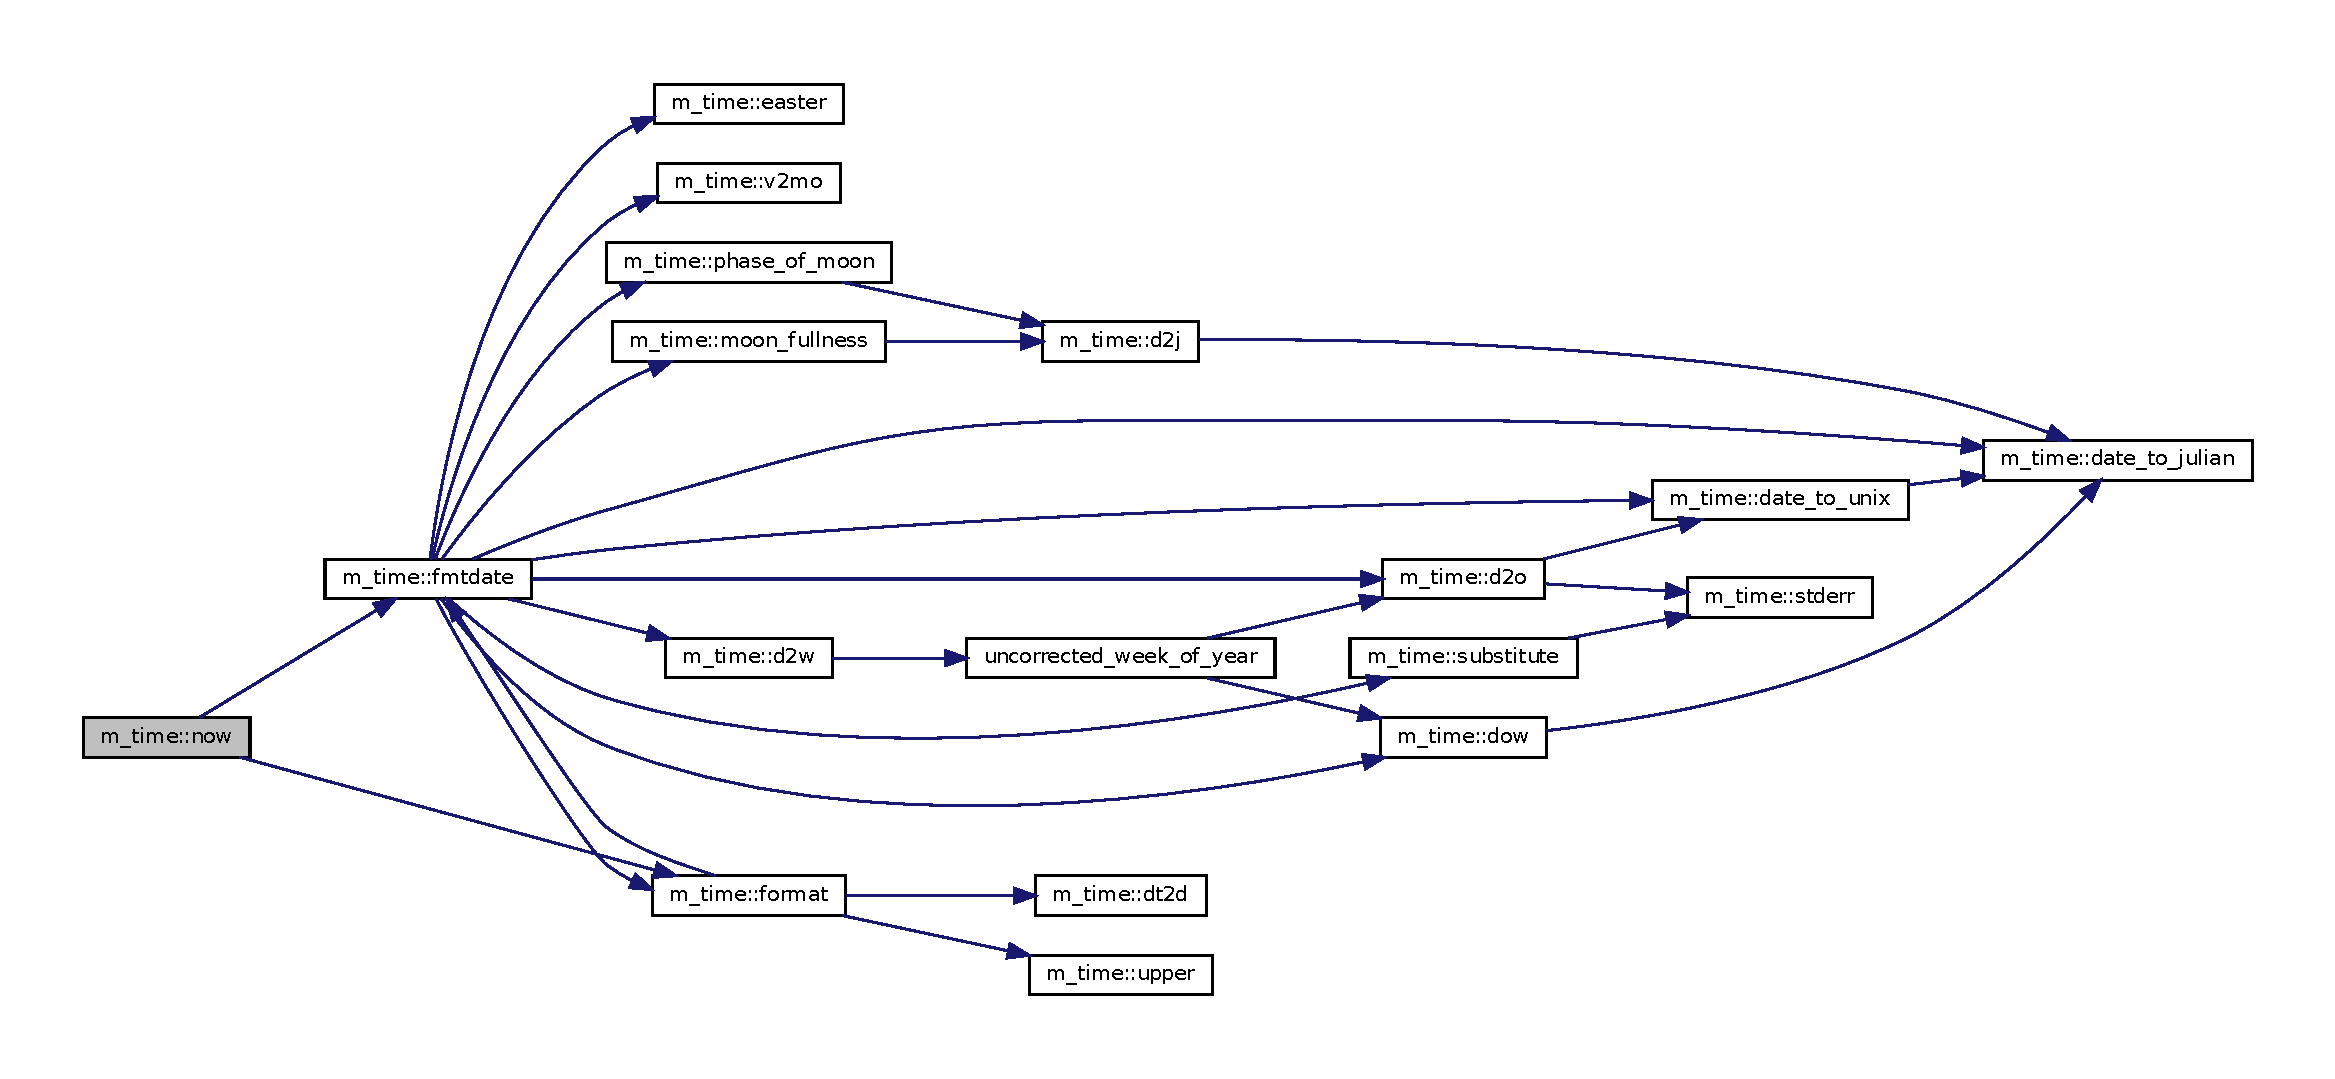
\includegraphics[width=350pt]{namespacem__time_a6b5e87be0e510ff268c1ecfbf67a3bdb_cgraph}
\end{center}
\end{figure}
Here is the caller graph for this function\+:\nopagebreak
\begin{figure}[H]
\begin{center}
\leavevmode
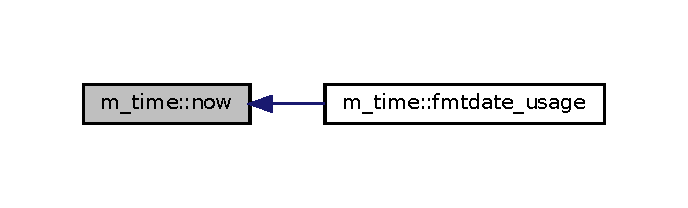
\includegraphics[width=330pt]{namespacem__time_a6b5e87be0e510ff268c1ecfbf67a3bdb_icgraph}
\end{center}
\end{figure}
\mbox{\Hypertarget{namespacem__time_a55e2cb9efc9d4d209ae2864f073d4f19}\label{namespacem__time_a55e2cb9efc9d4d209ae2864f073d4f19}} 
\index{m\_time@{m\_time}!o2d@{o2d}}
\index{o2d@{o2d}!m\_time@{m\_time}}
\doxysubsubsection{\texorpdfstring{o2d()}{o2d()}}
{\footnotesize\ttfamily integer function, dimension(8), public m\+\_\+time\+::o2d (\begin{DoxyParamCaption}\item[{integer, intent(in)}]{ordinal,  }\item[{integer, optional}]{year }\end{DoxyParamCaption})}

\hypertarget{namespacem__time_autotoc_md54}{}\doxysubsubsection{N\+A\+ME}\label{namespacem__time_autotoc_md54}
o2d(3f) -\/ \mbox{[}M\+\_\+time\+:O\+R\+D\+I\+N\+A\+L\+\_\+\+D\+AY\mbox{]} converts Ordinal day to D\+AT date-\/time array (L\+I\+C\+E\+N\+SE\+:PD)\hypertarget{namespacem__time_autotoc_md55}{}\doxysubsubsection{S\+Y\+N\+O\+P\+S\+IS}\label{namespacem__time_autotoc_md55}
\begin{DoxyVerb}function o2d(ordinal,[year]) result (dat)

 integer,intent(in) :: ordinal  ! the day of the year
 integer,optional   :: year     ! year
 integer            :: dat(8)   ! date time array
\end{DoxyVerb}
\hypertarget{namespacem__time_autotoc_md56}{}\doxysubsubsection{D\+E\+S\+C\+R\+I\+P\+T\+I\+ON}\label{namespacem__time_autotoc_md56}
Given an Ordinal day of the year return a date in the form of a \char`\"{}\+D\+A\+T\char`\"{} array.\hypertarget{namespacem__time_autotoc_md57}{}\doxysubsubsection{O\+P\+T\+I\+O\+NS}\label{namespacem__time_autotoc_md57}
ordinal The day of the year for the given year, where Jan 1st=1.

year An optional year for the ordinal day. If not present the current year is assumed.\hypertarget{namespacem__time_autotoc_md58}{}\doxysubsubsection{R\+E\+T\+U\+R\+NS}\label{namespacem__time_autotoc_md58}
dat Integer array holding a \char`\"{}\+D\+A\+T\char`\"{} array, similar in structure to the array returned by the intrinsic D\+A\+T\+E\+\_\+\+A\+N\+D\+\_\+\+T\+I\+M\+E(3f)\+:

dat=\mbox{[} year,month,day,timezone,hour,\& \& minutes,seconds,milliseconds\mbox{]}

The timezone value is from the current time on the current platform.\hypertarget{namespacem__time_autotoc_md59}{}\doxysubsubsection{E\+X\+A\+M\+P\+LE}\label{namespacem__time_autotoc_md59}
\begin{DoxyVerb}Sample program:

 program demo_o2d
 use M_time, only : o2d,fmtdate
 implicit none
 integer :: year
    do year=2004,2008
       write(*,*)&
       & '100th day of ',year,' is ',fmtdate(o2d(100,year))
    enddo
    write(*,*)'100th day of this year is ',fmtdate(o2d(100))
 end program demo_o2d

results:

 100th day of 2004 is Friday, April 9th, 2004 ...
 00:00:00 PM UTC-02:40
 100th day of 2005 is Sunday, April 10th, 2005 ...
 00:00:00 PM UTC-02:40
 100th day of 2006 is Monday, April 10th, 2006 ...
 00:00:00 PM UTC-02:40
 100th day of 2007 is Tuesday, April 10th, 2007 ...
 00:00:00 PM UTC-02:40
 100th day of 2008 is Wednesday, April 9th, 2008 ...
 00:00:00 PM UTC-02:40
 100th day of this year is Saturday, April 9th, 2016 ...
 00:00:00 PM UTC-02:40
\end{DoxyVerb}
 \hypertarget{namespacem__time_autotoc_md60}{}\doxysubsubsection{A\+U\+T\+H\+OR}\label{namespacem__time_autotoc_md60}
John S. Urban, 2015 \hypertarget{namespacem__time_autotoc_md61}{}\doxysubsubsection{L\+I\+C\+E\+N\+SE}\label{namespacem__time_autotoc_md61}
Public Domain 

References date\+\_\+to\+\_\+unix(), get\+\_\+timezone(), m\+\_\+time\+\_\+duplicate\+::stderr(), and u2d().

Here is the call graph for this function\+:\nopagebreak
\begin{figure}[H]
\begin{center}
\leavevmode
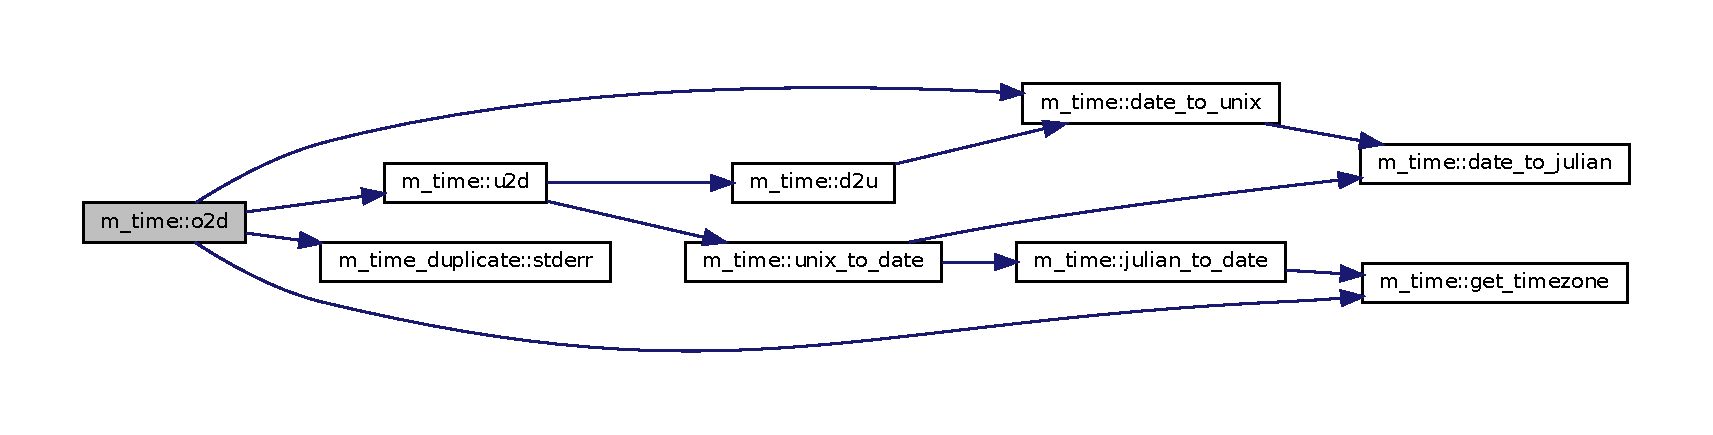
\includegraphics[width=350pt]{namespacem__time_a55e2cb9efc9d4d209ae2864f073d4f19_cgraph}
\end{center}
\end{figure}
Here is the caller graph for this function\+:\nopagebreak
\begin{figure}[H]
\begin{center}
\leavevmode
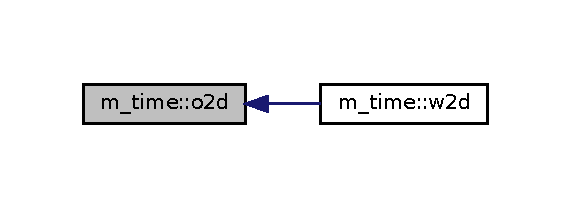
\includegraphics[width=274pt]{namespacem__time_a55e2cb9efc9d4d209ae2864f073d4f19_icgraph}
\end{center}
\end{figure}
\mbox{\Hypertarget{namespacem__time_ab8960d2aa60e134bcf77247d8b257963}\label{namespacem__time_ab8960d2aa60e134bcf77247d8b257963}} 
\index{m\_time@{m\_time}!ordinal\_seconds@{ordinal\_seconds}}
\index{ordinal\_seconds@{ordinal\_seconds}!m\_time@{m\_time}}
\doxysubsubsection{\texorpdfstring{ordinal\_seconds()}{ordinal\_seconds()}}
{\footnotesize\ttfamily integer function, public m\+\_\+time\+::ordinal\+\_\+seconds}

\hypertarget{namespacem__time_autotoc_md42}{}\doxysubsubsection{N\+A\+ME}\label{namespacem__time_autotoc_md42}
ordinal\+\_\+seconds(3f) -\/ \mbox{[}M\+\_\+time\+:O\+R\+D\+I\+N\+A\+L\+\_\+\+D\+AY\mbox{]} seconds since beginning of year (L\+I\+C\+E\+N\+SE\+:PD) \hypertarget{namespacem__time_autotoc_md43}{}\doxysubsubsection{S\+Y\+N\+O\+P\+S\+IS}\label{namespacem__time_autotoc_md43}
\begin{DoxyVerb}function ordinal_seconds()

 integer :: ordinal_seconds
\end{DoxyVerb}
 \hypertarget{namespacem__time_autotoc_md44}{}\doxysubsubsection{D\+E\+S\+C\+R\+I\+P\+T\+I\+ON}\label{namespacem__time_autotoc_md44}
Return number of seconds since beginning of current year.

Before using this routine consider the consequences if the application is running at the moment a new year begins.\hypertarget{namespacem__time_autotoc_md45}{}\doxysubsubsection{E\+X\+A\+M\+P\+LE}\label{namespacem__time_autotoc_md45}
\begin{DoxyVerb}sample program

 program demo_ordinal_seconds
 use M_time, only : ordinal_seconds
 implicit none
 character(len=1) :: paws
 integer          :: ios
 integer          :: istart, iend
 istart=ordinal_seconds()
 write(*,'(a)',advance='no')'now pause. Enter return to continue ...'
 read(*,'(a)',iostat=ios) paws
 iend=ordinal_seconds()
 write(*,*)'that took ',iend-istart,'seconds'
 write(*,*)istart,iend
 end program demo_ordinal_seconds
\end{DoxyVerb}
 \hypertarget{namespacem__time_autotoc_md46}{}\doxysubsubsection{A\+U\+T\+H\+OR}\label{namespacem__time_autotoc_md46}
John S. Urban, 2015 \hypertarget{namespacem__time_autotoc_md47}{}\doxysubsubsection{L\+I\+C\+E\+N\+SE}\label{namespacem__time_autotoc_md47}
Public Domain 

References d2o().

Here is the call graph for this function\+:\nopagebreak
\begin{figure}[H]
\begin{center}
\leavevmode
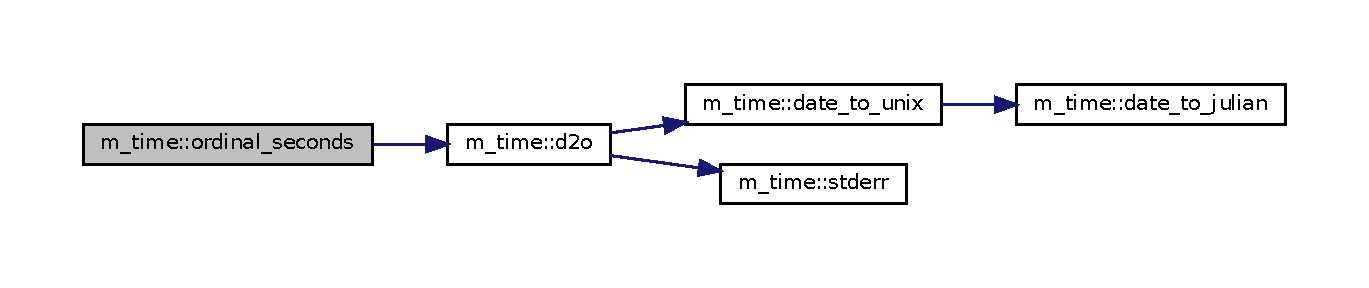
\includegraphics[width=350pt]{namespacem__time_ab8960d2aa60e134bcf77247d8b257963_cgraph}
\end{center}
\end{figure}
\mbox{\Hypertarget{namespacem__time_aa4dca4409bf20a011bb04988c1335d63}\label{namespacem__time_aa4dca4409bf20a011bb04988c1335d63}} 
\index{m\_time@{m\_time}!ordinal\_to\_date@{ordinal\_to\_date}}
\index{ordinal\_to\_date@{ordinal\_to\_date}!m\_time@{m\_time}}
\doxysubsubsection{\texorpdfstring{ordinal\_to\_date()}{ordinal\_to\_date()}}
{\footnotesize\ttfamily subroutine, public m\+\_\+time\+::ordinal\+\_\+to\+\_\+date (\begin{DoxyParamCaption}\item[{integer}]{yyyy,  }\item[{integer}]{ddd,  }\item[{integer, dimension(8)}]{dat }\end{DoxyParamCaption})}

\hypertarget{namespacem__time_autotoc_md48}{}\doxysubsubsection{N\+A\+ME}\label{namespacem__time_autotoc_md48}
ordinal\+\_\+to\+\_\+date(3f) -\/ \mbox{[}M\+\_\+time\+:O\+R\+D\+I\+N\+A\+L\+\_\+\+D\+AY\mbox{]} when given a valid year and day of the year returns the D\+AT array for the date (L\+I\+C\+E\+N\+SE\+:PD) \hypertarget{namespacem__time_autotoc_md49}{}\doxysubsubsection{S\+Y\+N\+O\+P\+S\+IS}\label{namespacem__time_autotoc_md49}
\begin{DoxyVerb}  subroutine ordinal_to_date(yyyy, ddd, dat)

   integer, intent(in)   :: yyyy
   integer, intent(in)   :: ddd
   integer, intent(out)  :: dat
\end{DoxyVerb}
 \hypertarget{namespacem__time_autotoc_md50}{}\doxysubsubsection{D\+E\+S\+C\+R\+I\+P\+T\+I\+ON}\label{namespacem__time_autotoc_md50}
When given a valid year, Y\+Y\+YY, and day of the year, D\+DD, returns the date as a D\+AT date array \hypertarget{namespacem__time_autotoc_md51}{}\doxysubsubsection{O\+P\+T\+I\+O\+NS}\label{namespacem__time_autotoc_md51}
yyyy known year ddd known ordinal day of the year \hypertarget{namespacem__time_autotoc_md52}{}\doxysubsubsection{R\+E\+T\+U\+R\+NS}\label{namespacem__time_autotoc_md52}
dat D\+AT array describing the date \hypertarget{namespacem__time_autotoc_md53}{}\doxysubsubsection{E\+X\+A\+M\+P\+LE}\label{namespacem__time_autotoc_md53}
\begin{DoxyVerb}Sample program:

 program demo_ordinal_to_date
 use M_time, only : ordinal_to_date
 implicit none
 INTEGER            :: yyyy, ddd, mm, dd, yy
 integer            :: dat(8)
 integer            :: ios
   INFINITE: do
      write(*,'(a)',advance='no')&
      & 'Enter year YYYY and ordinal day of year DD '
      read(*,*,iostat=ios)yyyy,ddd
      if(ios.ne.0)exit INFINITE
      ! recover month and day from year and day number.
      call ordinal_to_date(yyyy, ddd, dat)
      yy=dat(1)
      mm=dat(2)
      dd=dat(3)
      write(*,'(*(g0))')'For Year ',yyyy,' and Ordinal day ',ddd,  &
      &         ' Month is ',mm,' and Day of Month is ',dd, &
      &         ' and Year is ',yy
    enddo INFINITE
 end program demo_ordinal_to_date
\end{DoxyVerb}
 

References d2j(), j2d(), and realtime.

Here is the call graph for this function\+:\nopagebreak
\begin{figure}[H]
\begin{center}
\leavevmode
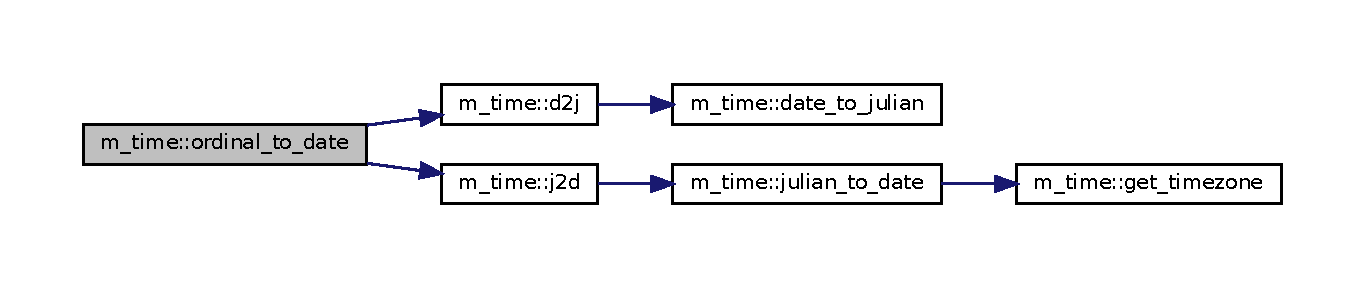
\includegraphics[width=350pt]{namespacem__time_aa4dca4409bf20a011bb04988c1335d63_cgraph}
\end{center}
\end{figure}
\mbox{\Hypertarget{namespacem__time_ab8a976e2f113cc38b6df80974cee55dc}\label{namespacem__time_ab8a976e2f113cc38b6df80974cee55dc}} 
\index{m\_time@{m\_time}!phase\_of\_moon@{phase\_of\_moon}}
\index{phase\_of\_moon@{phase\_of\_moon}!m\_time@{m\_time}}
\doxysubsubsection{\texorpdfstring{phase\_of\_moon()}{phase\_of\_moon()}}
{\footnotesize\ttfamily character(len=\+:) function, allocatable, public m\+\_\+time\+::phase\+\_\+of\+\_\+moon (\begin{DoxyParamCaption}\item[{integer, dimension(8), intent(in)}]{datin }\end{DoxyParamCaption})}

\hypertarget{namespacem__time_autotoc_md208}{}\doxysubsubsection{N\+A\+ME}\label{namespacem__time_autotoc_md208}
phase\+\_\+of\+\_\+moon(3f) -\/ \mbox{[}M\+\_\+time\+:A\+S\+T\+R\+O\+L\+O\+G\+I\+C\+AL\mbox{]} return name for phase of moon for given date (L\+I\+C\+E\+N\+SE\+:PD) \hypertarget{namespacem__time_autotoc_md209}{}\doxysubsubsection{S\+Y\+N\+O\+P\+S\+IS}\label{namespacem__time_autotoc_md209}
function phase\+\_\+of\+\_\+moon(datin)

integer,intent(in) \+:: datin(8) character(len=\+:),allocatable \+:: phase\+\_\+of\+\_\+moon\hypertarget{namespacem__time_autotoc_md210}{}\doxysubsubsection{D\+E\+S\+C\+R\+I\+P\+T\+I\+ON}\label{namespacem__time_autotoc_md210}
Phases Of The Moon

This procedure is used to support the p field descriptor for the fmtdate(3f) routine.

The moon circles the earth every 29.\+530588853 days on average, so pick a starting point and count. A new moon occurred at Julian date 2451550.\+1 (January 6, 2000, 18\+:14 U\+TC). Then it is easy to count the number of days since the last new moon. This is an approximate calculation.

There are eight generally recognized phases of the moon in common use

o new or dark o waxing crescent o first quarter o waxing gibbous o full o waning gibbous o last quarter o waning crescent

To calculate the phase of the moon simply divide the days since the last new moon by eight and select the appropriate phase.

Note that technically the four states (new, first quarter, full, third quarter) are events not phases. That is to say, the moon is technically only new for an instant.\hypertarget{namespacem__time_autotoc_md211}{}\doxysubsubsection{E\+X\+A\+M\+P\+L\+ES}\label{namespacem__time_autotoc_md211}
Sample\+:

program demo\+\_\+phase\+\_\+of\+\_\+moon use M\+\_\+time, only \+: now use M\+\_\+time, only \+: phase\+\_\+of\+\_\+moon use M\+\_\+time, only \+: moon\+\_\+fullness implicit none integer \+:: dat(8) ! generate D\+AT array call date\+\_\+and\+\_\+time(values=dat) ! show D\+AT array write($\ast$,\textquotesingle{}(\char`\"{} Today is\+:\char`\"{},$\ast$(i0\+:,\char`\"{}\+:\char`\"{}))\textquotesingle{})dat ! the p and P fields are supported by fmtdate(3f) write($\ast$,$\ast$)\& \& now(\textquotesingle{}The phase of the moon is p, with a fullness of P\textquotesingle{}) write($\ast$,\textquotesingle{}(1x,$\ast$(a))\textquotesingle{},advance=\textquotesingle{}no\textquotesingle{})\& \& \textquotesingle{}The phase of the moon is \textquotesingle{},trim( phase\+\_\+of\+\_\+moon(dat)),\textquotesingle{},\textquotesingle{} write($\ast$,\textquotesingle{}(1x,a,i0,a)\textquotesingle{})\textquotesingle{}with a fullness of \textquotesingle{},moon\+\_\+fullness(dat),\textquotesingle{}\textquotesingle{} end program demo\+\_\+phase\+\_\+of\+\_\+moon

Sample output\+:

Today is\+:2018\+:11\+:3\+:-\/240\+:20\+:18\+:44\+:245 The phase of the moon is Waning crescent, with a fullness of -\/30\% The phase of the moon is Waning crescent, with a fullness of -\/30\%\hypertarget{namespacem__time_autotoc_md212}{}\doxysubsubsection{A\+U\+T\+H\+OR}\label{namespacem__time_autotoc_md212}
John S. Urban, 2015 \hypertarget{namespacem__time_autotoc_md213}{}\doxysubsubsection{L\+I\+C\+E\+N\+SE}\label{namespacem__time_autotoc_md213}
Public Domain 

References d2j().

Here is the call graph for this function\+:\nopagebreak
\begin{figure}[H]
\begin{center}
\leavevmode
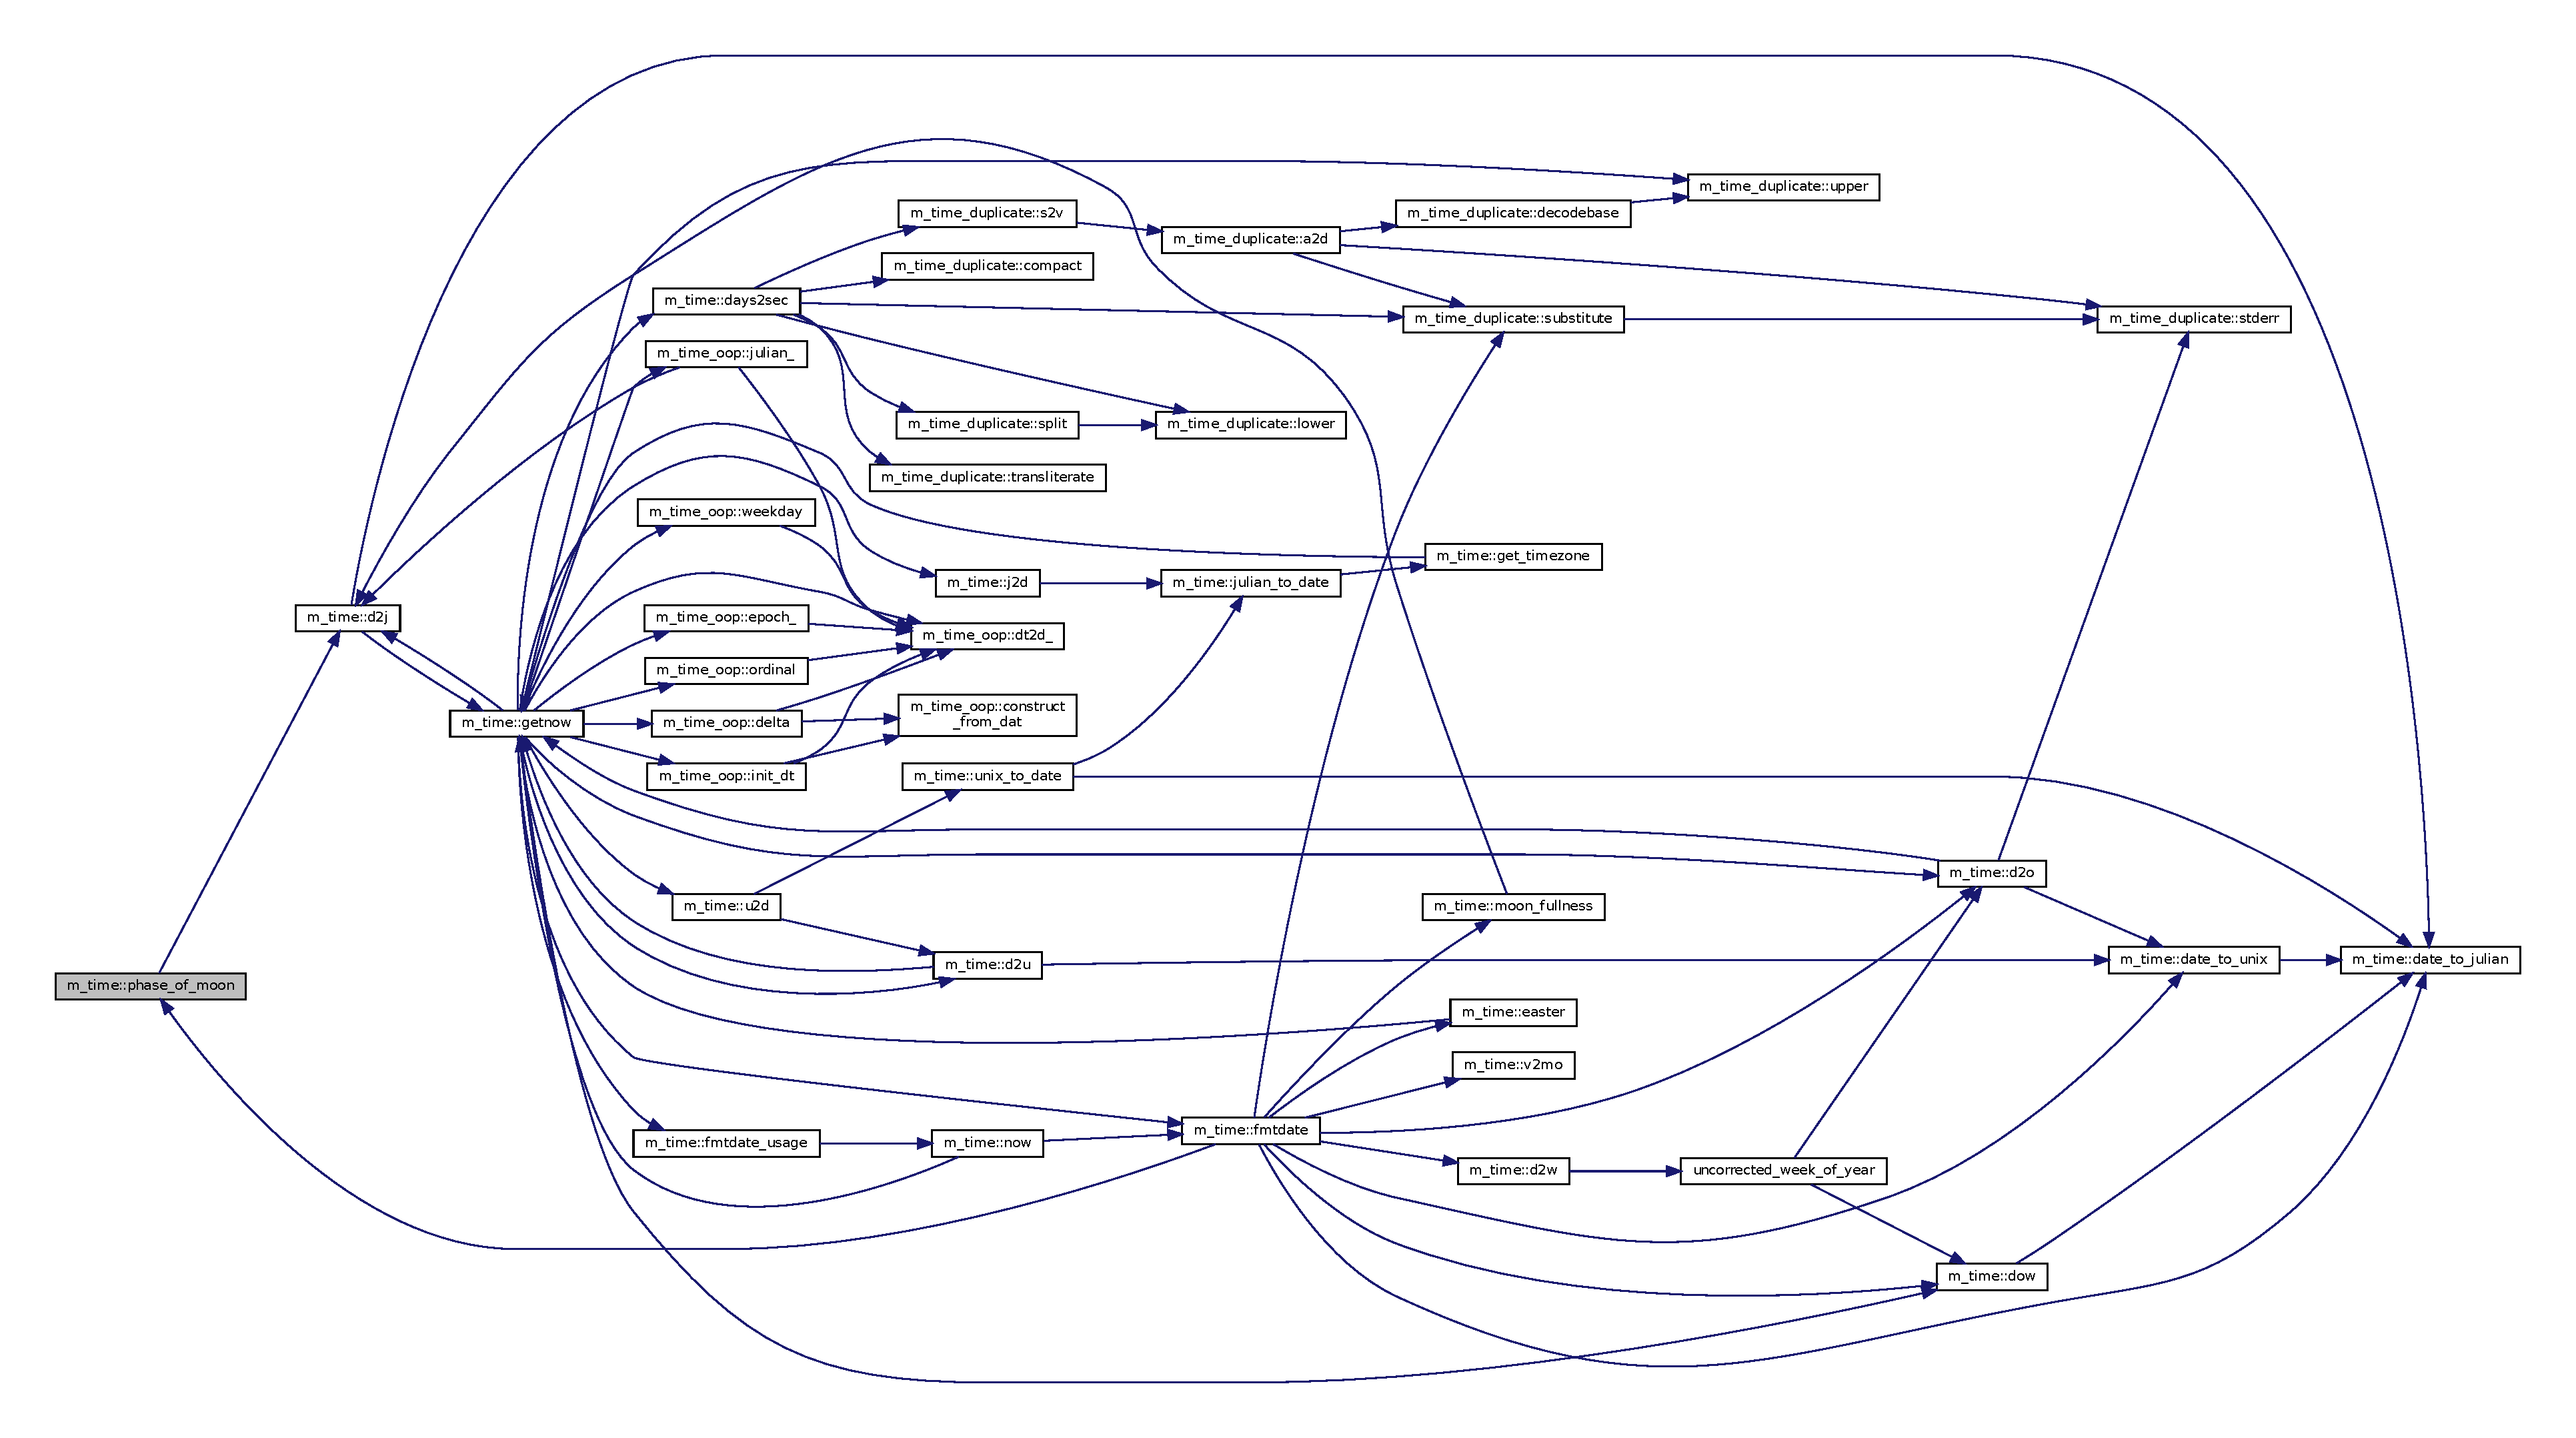
\includegraphics[width=350pt]{namespacem__time_ab8a976e2f113cc38b6df80974cee55dc_cgraph}
\end{center}
\end{figure}
Here is the caller graph for this function\+:\nopagebreak
\begin{figure}[H]
\begin{center}
\leavevmode
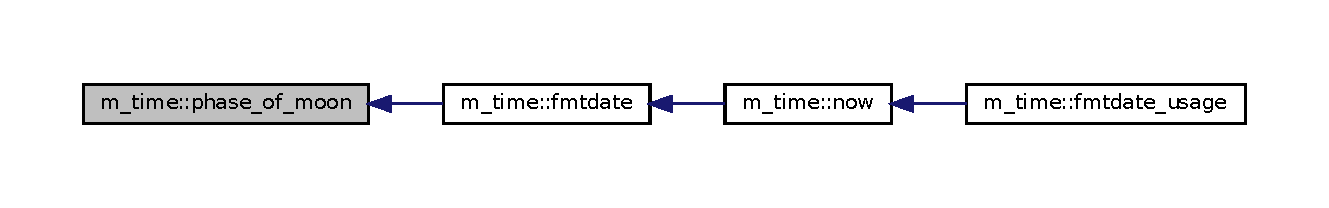
\includegraphics[width=350pt]{namespacem__time_ab8a976e2f113cc38b6df80974cee55dc_icgraph}
\end{center}
\end{figure}
\mbox{\Hypertarget{namespacem__time_a7788285d79b8d58323b05e9a30a2d992}\label{namespacem__time_a7788285d79b8d58323b05e9a30a2d992}} 
\index{m\_time@{m\_time}!sec2days@{sec2days}}
\index{sec2days@{sec2days}!m\_time@{m\_time}}
\doxysubsubsection{\texorpdfstring{sec2days()}{sec2days()}}
{\footnotesize\ttfamily character(len=\+:) function, allocatable, public m\+\_\+time\+::sec2days (\begin{DoxyParamCaption}\item[{class($\ast$), intent(in)}]{seconds,  }\item[{logical, intent(in), optional}]{crop }\end{DoxyParamCaption})}

\hypertarget{namespacem__time_autotoc_md192}{}\doxysubsubsection{N\+A\+ME}\label{namespacem__time_autotoc_md192}
sec2days(3f) -\/ \mbox{[}M\+\_\+time\+:D\+U\+R\+A\+T\+I\+ON\mbox{]} convert seconds to string of form dd-\/hh\+:mm\+:ss (L\+I\+C\+E\+N\+SE\+:PD)\hypertarget{namespacem__time_autotoc_md193}{}\doxysubsubsection{S\+Y\+N\+O\+P\+S\+IS}\label{namespacem__time_autotoc_md193}
\begin{DoxyVerb}function sec2days(seconds,crop) result(dhms)

 real(kind=realtime),intent(in) :: seconds
   or
 integer,intent(in)             :: seconds
   or
 real,intent(in)                :: seconds
   or
 character(len=*)               :: seconds

 logical,intent(in),optional    :: crop
 character(len=:),allocatable   :: dhms
\end{DoxyVerb}
\hypertarget{namespacem__time_autotoc_md194}{}\doxysubsubsection{D\+E\+S\+C\+R\+I\+P\+T\+I\+ON}\label{namespacem__time_autotoc_md194}
Given a number of seconds convert it to a string of the form \begin{DoxyVerb}dd-hh:mm:ss
\end{DoxyVerb}


where dd is days, hh hours, mm minutes and ss seconds.\hypertarget{namespacem__time_autotoc_md195}{}\doxysubsubsection{O\+P\+T\+I\+O\+NS}\label{namespacem__time_autotoc_md195}
seconds number of seconds to convert to string of form dd-\/hh\+:mm\+:ss. May be of type I\+N\+T\+E\+G\+ER, R\+E\+AL, R\+E\+AL(K\+I\+ND=R\+E\+A\+L\+T\+I\+ME), or C\+H\+A\+R\+A\+C\+T\+ER.

C\+H\+A\+R\+A\+C\+T\+ER strings may be of the form \mbox{[}N\+Nd\mbox{]}\mbox{[}N\+Nh\mbox{]}\mbox{[}N\+Nm\mbox{]}\mbox{[}N\+Ns\mbox{]}\mbox{[}N\+Nw\mbox{]}. Case,spaces and underscores are ignored. Allowed aliases for d,h,m, and s units are \begin{DoxyVerb}d -  days,day
m -  minutes,minute,min
h -  hours,hour,hrs,hr
s -  seconds,second,sec
\end{DoxyVerb}


The numeric values may represent floating point numbers.

crop if .true., remove leading zero day values or day and hour values. Optional, defaults to .false. . \hypertarget{namespacem__time_autotoc_md196}{}\doxysubsubsection{R\+E\+T\+U\+R\+NS}\label{namespacem__time_autotoc_md196}
dmhs the returned string of form \mbox{[}d\+:h\+:\mbox{]}m\+:s\hypertarget{namespacem__time_autotoc_md197}{}\doxysubsubsection{E\+X\+A\+M\+P\+LE}\label{namespacem__time_autotoc_md197}
\begin{DoxyVerb}Sample Program:

 program demo_sec2days
 use M_time, only : sec2days
 implicit none
    write(*,*)sec2days(129860)
    write(*,*)sec2days(80000.0d0)
    write(*,*)sec2days(80000.0,crop=.true.)
    write(*,*)sec2days('1 day 2.0hr 100 min 300.0seconds')
 end program demo_sec2days

results:

 1-12:04:20
 0-22:13:20
 22:13:20
 1-03:45:00
\end{DoxyVerb}
\hypertarget{namespacem__time_autotoc_md198}{}\doxysubsubsection{A\+U\+T\+H\+OR}\label{namespacem__time_autotoc_md198}
John S. Urban, 2015 \hypertarget{namespacem__time_autotoc_md199}{}\doxysubsubsection{L\+I\+C\+E\+N\+SE}\label{namespacem__time_autotoc_md199}
Public Domain 

References m\+\_\+time\+\_\+duplicate\+::compact(), m\+\_\+time\+\_\+duplicate\+::lower(), realtime, m\+\_\+time\+\_\+duplicate\+::s2v(), m\+\_\+time\+\_\+duplicate\+::split(), m\+\_\+time\+\_\+duplicate\+::substitute(), and m\+\_\+time\+\_\+duplicate\+::transliterate().

Here is the call graph for this function\+:\nopagebreak
\begin{figure}[H]
\begin{center}
\leavevmode
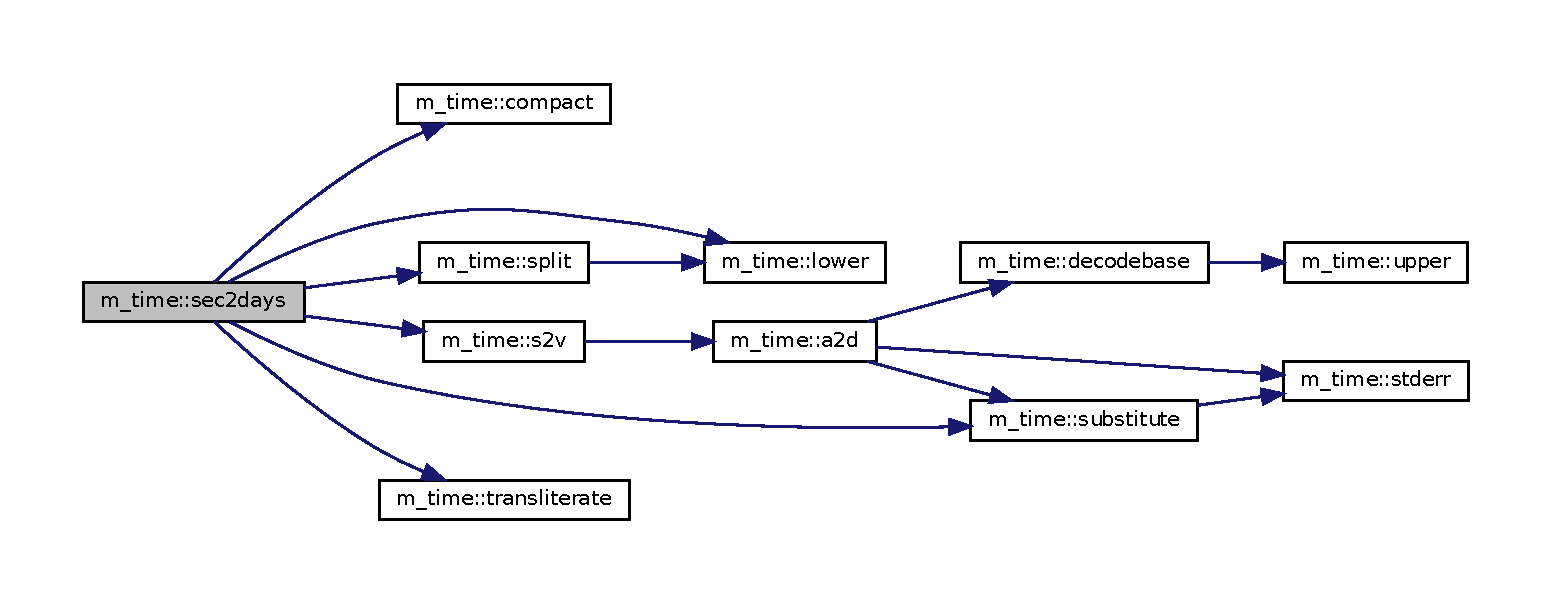
\includegraphics[width=350pt]{namespacem__time_a7788285d79b8d58323b05e9a30a2d992_cgraph}
\end{center}
\end{figure}
\mbox{\Hypertarget{namespacem__time_a7c5d028ae1e1e01162ffc7bb55dcbbb1}\label{namespacem__time_a7c5d028ae1e1e01162ffc7bb55dcbbb1}} 
\index{m\_time@{m\_time}!system\_sleep@{system\_sleep}}
\index{system\_sleep@{system\_sleep}!m\_time@{m\_time}}
\doxysubsubsection{\texorpdfstring{system\_sleep()}{system\_sleep()}}
{\footnotesize\ttfamily subroutine, public m\+\_\+time\+::system\+\_\+sleep (\begin{DoxyParamCaption}\item[{class($\ast$), intent(in)}]{seconds }\end{DoxyParamCaption})}

\hypertarget{namespacem__time_autotoc_md228}{}\doxysubsubsection{N\+A\+ME}\label{namespacem__time_autotoc_md228}
system\+\_\+sleep(3f) -\/ \mbox{[}M\+\_\+time\+:C\+\_\+\+I\+N\+T\+E\+R\+F\+A\+CE\mbox{]} call C sleep(3c) or usleep(3c) procedure (L\+I\+C\+E\+N\+SE\+:PD) \hypertarget{namespacem__time_autotoc_md229}{}\doxysubsubsection{S\+Y\+N\+O\+P\+S\+IS}\label{namespacem__time_autotoc_md229}
\begin{DoxyVerb}subroutine system_sleep(wait_seconds)

   integer,intent(in)  :: wait_seconds
      or
   real,intent(in)  :: wait_seconds
\end{DoxyVerb}
\hypertarget{namespacem__time_autotoc_md230}{}\doxysubsubsection{D\+E\+S\+C\+R\+I\+P\+T\+I\+ON}\label{namespacem__time_autotoc_md230}
The system\+\_\+sleep(3f) routine uses the intrinsic I\+S\+O\+\_\+\+C\+\_\+\+B\+I\+N\+D\+I\+NG interface to call the C sleep(3c) procedure or usleep(3c) routine.\hypertarget{namespacem__time_autotoc_md231}{}\doxysubsubsection{O\+P\+T\+I\+O\+NS}\label{namespacem__time_autotoc_md231}
wait\+\_\+seconds integer,real or doubleprecision number of seconds for process to sleep.\hypertarget{namespacem__time_autotoc_md232}{}\doxysubsubsection{E\+X\+A\+M\+P\+LE}\label{namespacem__time_autotoc_md232}
\begin{DoxyVerb}Sample program:

 program demo_system_sleep
 use M_time, only : system_sleep, now
 implicit none
 integer :: i
    !
    write(*,'(a)')"Time before integer call is: ",now()
    call system_sleep(4)
    write(*,'(a)')"Time after  integer call is: ",now()
    !
    write(*,'(a)')"Time before real call is: ",now()
    call system_sleep(4.0)
    write(*,'(a)')"Time after  real call is: ",now()
    !
    write(*,'(a)')"Time before loop is: ",now()
    do i=1,1000
       call system_sleep(4.0/1000.0)
    enddo
    write(*,'(a)')"Time after loop  is: ",now()
    !
 end program demo_system_sleep
\end{DoxyVerb}


results \begin{DoxyVerb}Time before integer call is:
Sunday, July 17th, 2016 2:29:45 AM UTC-0240
Time after integer call is:
Sunday, July 17th, 2016 2:29:49 AM UTC-0240
Time before real call is:
Sunday, July 17th, 2016 2:29:49 AM UTC-0240
Time after  real call is:
Sunday, July 17th, 2016 2:29:53 AM UTC-0240
Time before loop is:
Sunday, July 17th, 2016 2:29:53 AM UTC-0240
Time after loop  is:
Sunday, July 17th, 2016 2:30:09 AM UTC-0240
\end{DoxyVerb}
\hypertarget{namespacem__time_autotoc_md233}{}\doxysubsubsection{A\+U\+T\+H\+OR}\label{namespacem__time_autotoc_md233}
John S. Urban, 2015\hypertarget{namespacem__time_autotoc_md234}{}\doxysubsubsection{L\+I\+C\+E\+N\+SE}\label{namespacem__time_autotoc_md234}
Public Domain 

References call\+\_\+sleep(), call\+\_\+usleep(), and realtime.

Here is the call graph for this function\+:\nopagebreak
\begin{figure}[H]
\begin{center}
\leavevmode
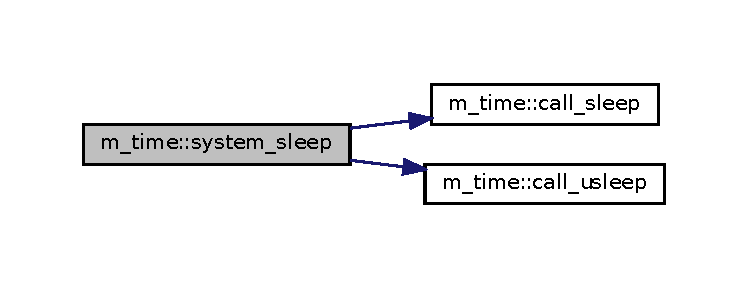
\includegraphics[width=350pt]{namespacem__time_a7c5d028ae1e1e01162ffc7bb55dcbbb1_cgraph}
\end{center}
\end{figure}
\mbox{\Hypertarget{namespacem__time_a083bc231f8ba1879d7f86ab424e77d6c}\label{namespacem__time_a083bc231f8ba1879d7f86ab424e77d6c}} 
\index{m\_time@{m\_time}!u2d@{u2d}}
\index{u2d@{u2d}!m\_time@{m\_time}}
\doxysubsubsection{\texorpdfstring{u2d()}{u2d()}}
{\footnotesize\ttfamily integer function, dimension(8), public m\+\_\+time\+::u2d (\begin{DoxyParamCaption}\item[{class($\ast$), intent(in), optional}]{unixtime }\end{DoxyParamCaption})}

\hypertarget{namespacem__time_autotoc_md184}{}\doxysubsubsection{N\+A\+ME}\label{namespacem__time_autotoc_md184}
u2d(3f) -\/ \mbox{[}M\+\_\+time\+:U\+N\+I\+X\+\_\+\+E\+P\+O\+CH\mbox{]} given Unix Epoch Time returns D\+AT date-\/time array (L\+I\+C\+E\+N\+SE\+:PD)\hypertarget{namespacem__time_autotoc_md185}{}\doxysubsubsection{S\+Y\+N\+O\+P\+S\+IS}\label{namespacem__time_autotoc_md185}
\begin{DoxyVerb}function u2d(unixtime) result (dat)

 class(*),intent(in),optional      :: unixtime
 ! integer
 ! real
 ! real(kind=realtime)

 integer                           :: dat(8)
\end{DoxyVerb}
\hypertarget{namespacem__time_autotoc_md186}{}\doxysubsubsection{D\+E\+S\+C\+R\+I\+P\+T\+I\+ON}\label{namespacem__time_autotoc_md186}
Given Unix Epoch Time returns D\+AT date-\/time array\hypertarget{namespacem__time_autotoc_md187}{}\doxysubsubsection{O\+P\+T\+I\+O\+NS}\label{namespacem__time_autotoc_md187}
unixtime The \char`\"{}\+Unix Epoch\char`\"{} time, or the number of seconds since 00\+:00\+:00 on January 1st, 1970, U\+TC. If not present, use current time.\hypertarget{namespacem__time_autotoc_md188}{}\doxysubsubsection{R\+E\+T\+U\+R\+NS}\label{namespacem__time_autotoc_md188}
dat Integer array holding a \char`\"{}\+D\+A\+T\char`\"{} array, similar in structure to the array returned by the intrinsic D\+A\+T\+E\+\_\+\+A\+N\+D\+\_\+\+T\+I\+M\+E(3f)\+:

dat=\mbox{[} year,month,day,timezone,hour,\& \& minutes,seconds,milliseconds\mbox{]}\hypertarget{namespacem__time_autotoc_md189}{}\doxysubsubsection{E\+X\+A\+M\+P\+LE}\label{namespacem__time_autotoc_md189}
\begin{DoxyVerb}Sample program:

 program demo_u2d
 use M_time, only : u2d, d2u, fmtdate, realtime
 implicit none
 real(kind=realtime) :: today
 integer :: dat(8)
    ! get the date using intrinsic
    call date_and_time(values=dat)
    ! convert today to Julian Date
    today=d2u(dat)
    write(*,*)'Today=',fmtdate(u2d(today))
    ! subtract day
    write(*,*)'Yesterday=',fmtdate(u2d(today-86400.0d0))
    ! add day
    write(*,*)'Tomorrow=',fmtdate(u2d(today+86400.0d0))
 end program demo_u2d

results:

 Today=Tuesday, July 19th, 2016 11:10:08 AM
 Yesterday=Monday, July 18th, 2016 11:10:08 AM
 Tomorrow=Wednesday, July 20th, 2016 11:10:08 AM
\end{DoxyVerb}
\hypertarget{namespacem__time_autotoc_md190}{}\doxysubsubsection{A\+U\+T\+H\+OR}\label{namespacem__time_autotoc_md190}
John S. Urban, 2015 \hypertarget{namespacem__time_autotoc_md191}{}\doxysubsubsection{L\+I\+C\+E\+N\+SE}\label{namespacem__time_autotoc_md191}
Public Domain 

References d2u(), realtime, and unix\+\_\+to\+\_\+date().

Here is the call graph for this function\+:\nopagebreak
\begin{figure}[H]
\begin{center}
\leavevmode
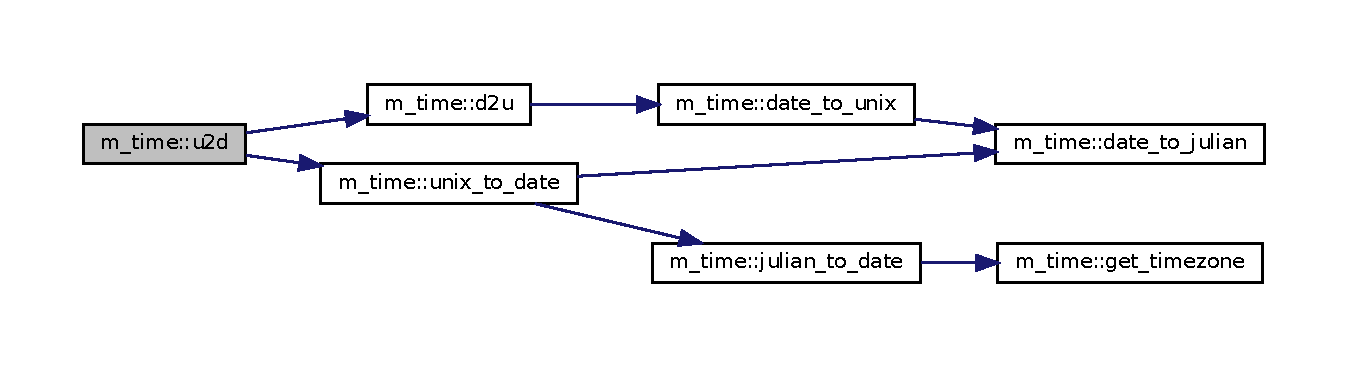
\includegraphics[width=350pt]{namespacem__time_a083bc231f8ba1879d7f86ab424e77d6c_cgraph}
\end{center}
\end{figure}
Here is the caller graph for this function\+:\nopagebreak
\begin{figure}[H]
\begin{center}
\leavevmode
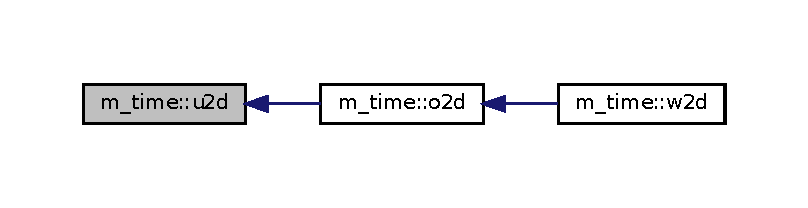
\includegraphics[width=350pt]{namespacem__time_a083bc231f8ba1879d7f86ab424e77d6c_icgraph}
\end{center}
\end{figure}
\mbox{\Hypertarget{namespacem__time_acc62ada23f8fa2fe67b428702fbcbf1c}\label{namespacem__time_acc62ada23f8fa2fe67b428702fbcbf1c}} 
\index{m\_time@{m\_time}!unix\_to\_date@{unix\_to\_date}}
\index{unix\_to\_date@{unix\_to\_date}!m\_time@{m\_time}}
\doxysubsubsection{\texorpdfstring{unix\_to\_date()}{unix\_to\_date()}}
{\footnotesize\ttfamily subroutine, public m\+\_\+time\+::unix\+\_\+to\+\_\+date (\begin{DoxyParamCaption}\item[{class($\ast$), intent(in)}]{unixtime,  }\item[{integer, dimension(8), intent(out)}]{dat,  }\item[{integer, intent(out)}]{ierr }\end{DoxyParamCaption})}

\hypertarget{namespacem__time_autotoc_md26}{}\doxysubsubsection{N\+A\+ME}\label{namespacem__time_autotoc_md26}
unix\+\_\+to\+\_\+date(3f) -\/ \mbox{[}M\+\_\+time\+:U\+N\+I\+X\+\_\+\+E\+P\+O\+CH\mbox{]} converts Unix Epoch Time to D\+AT date-\/time array (L\+I\+C\+E\+N\+SE\+:PD)\hypertarget{namespacem__time_autotoc_md27}{}\doxysubsubsection{S\+Y\+N\+O\+P\+S\+IS}\label{namespacem__time_autotoc_md27}
\begin{DoxyVerb}subroutine unix_to_date(unixtime,dat,ierr)

 real(kind=realtime),intent(in) :: unixtime
 integer,intent(out)            :: dat(8)
 integer,intent(out)            :: ierr
\end{DoxyVerb}
\hypertarget{namespacem__time_autotoc_md28}{}\doxysubsubsection{D\+E\+S\+C\+R\+I\+P\+T\+I\+ON}\label{namespacem__time_autotoc_md28}
Converts a Unix Epoch Time (U\+ET) to a D\+AT date-\/time array.\hypertarget{namespacem__time_autotoc_md29}{}\doxysubsubsection{O\+P\+T\+I\+O\+NS}\label{namespacem__time_autotoc_md29}
\begin{DoxyVerb}unixtime  The "Unix Epoch" time, or the number of seconds since
          00:00:00 on January 1st, 1970, UTC; of type
          real(kind=realtime).
\end{DoxyVerb}
\hypertarget{namespacem__time_autotoc_md30}{}\doxysubsubsection{R\+E\+T\+U\+R\+NS}\label{namespacem__time_autotoc_md30}
dat Integer array holding a \char`\"{}\+D\+A\+T\char`\"{} array, similar in structure to the array returned by the intrinsic D\+A\+T\+E\+\_\+\+A\+N\+D\+\_\+\+T\+I\+M\+E(3f)\+:

dat=\mbox{[} year,month,day,timezone,hour,\& \& minutes,seconds,milliseconds\mbox{]}

ierr Error code. If 0 no error occurred.\hypertarget{namespacem__time_autotoc_md31}{}\doxysubsubsection{E\+X\+A\+M\+P\+LE}\label{namespacem__time_autotoc_md31}
\begin{DoxyVerb} Sample program:

  program demo_unix_to_date
  use M_time, only : unix_to_date, u2d, fmtdate, realtime
  implicit none
  real(kind=realtime)           :: unixtime
  ! seconds in a day
  real(kind=realtime),parameter :: DAY=86400.0d0
  integer                       :: dat(8)
  integer                       :: ierr
     ! sample Unix Epoch time
     unixtime=1468939038.4639933d0
     ! create DAT array for today
     call unix_to_date(unixtime,dat,ierr)
     write(*,*)'Sample Date=',fmtdate(dat)
     ! go back one day
     call unix_to_date(unixtime-DAY,dat,ierr)
     ! subtract day and print
     write(*,*)'Day Before =',fmtdate(dat)
     ! go forward one day
     call unix_to_date(unixtime+DAY,dat,ierr)
     ! add day print
     write(*,*)'Day After  =',fmtdate(dat)
  end program demo_unix_to_date

Results:

 Sample Date=Tuesday, July 19th, 2016 10:37:18 AM
 Day Before =Monday, July 18th, 2016 10:37:18 AM
 Day After  =Wednesday, July 20th, 2016 10:37:18 AM
\end{DoxyVerb}
\hypertarget{namespacem__time_autotoc_md32}{}\doxysubsubsection{A\+U\+T\+H\+OR}\label{namespacem__time_autotoc_md32}
John S. Urban, 2015 \hypertarget{namespacem__time_autotoc_md33}{}\doxysubsubsection{L\+I\+C\+E\+N\+SE}\label{namespacem__time_autotoc_md33}
Public Domain 

References date\+\_\+to\+\_\+julian(), julian\+\_\+to\+\_\+date(), realtime, and secday.

Here is the call graph for this function\+:\nopagebreak
\begin{figure}[H]
\begin{center}
\leavevmode
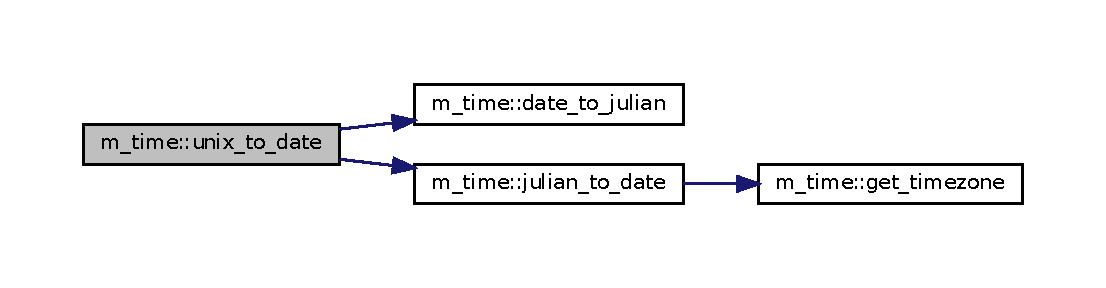
\includegraphics[width=350pt]{namespacem__time_acc62ada23f8fa2fe67b428702fbcbf1c_cgraph}
\end{center}
\end{figure}
Here is the caller graph for this function\+:\nopagebreak
\begin{figure}[H]
\begin{center}
\leavevmode
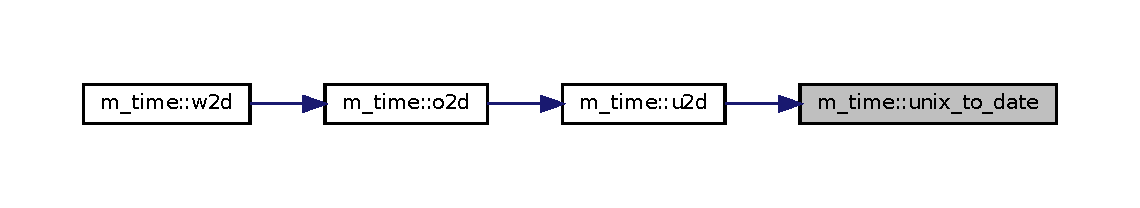
\includegraphics[width=350pt]{namespacem__time_acc62ada23f8fa2fe67b428702fbcbf1c_icgraph}
\end{center}
\end{figure}
\mbox{\Hypertarget{namespacem__time_a6f28cf00e4998bb50bb503f5e4bd3f77}\label{namespacem__time_a6f28cf00e4998bb50bb503f5e4bd3f77}} 
\index{m\_time@{m\_time}!v2mo@{v2mo}}
\index{v2mo@{v2mo}!m\_time@{m\_time}}
\doxysubsubsection{\texorpdfstring{v2mo()}{v2mo()}}
{\footnotesize\ttfamily character(len=\+:) function, allocatable, public m\+\_\+time\+::v2mo (\begin{DoxyParamCaption}\item[{integer, intent(in)}]{imonth }\end{DoxyParamCaption})}

\hypertarget{namespacem__time_autotoc_md62}{}\doxysubsubsection{N\+A\+ME}\label{namespacem__time_autotoc_md62}
v2mo(3f) -\/ \mbox{[}M\+\_\+time\+:M\+O\+N\+T\+H\+\_\+\+N\+A\+ME\mbox{]} returns the month name of a Common month number (L\+I\+C\+E\+N\+SE\+:PD)\hypertarget{namespacem__time_autotoc_md63}{}\doxysubsubsection{S\+Y\+N\+O\+P\+S\+IS}\label{namespacem__time_autotoc_md63}
\begin{DoxyVerb}function v2mo(imonth) result(month_name)

 integer,intent(in)           :: imonth      ! month number (1-12)
 character(len=:),allocatable :: month_name  ! month name
\end{DoxyVerb}
\hypertarget{namespacem__time_autotoc_md64}{}\doxysubsubsection{D\+E\+S\+C\+R\+I\+P\+T\+I\+ON}\label{namespacem__time_autotoc_md64}
Given a Common Calendar month number, return the name of the month as a string.\hypertarget{namespacem__time_autotoc_md65}{}\doxysubsubsection{O\+P\+T\+I\+O\+NS}\label{namespacem__time_autotoc_md65}
imonth Common month number (1-\/12). If out of the allowable range the month name returned will be \textquotesingle{}U\+N\+K\+N\+O\+WN\textquotesingle{}. \hypertarget{namespacem__time_autotoc_md66}{}\doxysubsubsection{R\+E\+T\+U\+R\+NS}\label{namespacem__time_autotoc_md66}
month\+\_\+name A string representing a month name or the word \textquotesingle{}U\+N\+K\+N\+O\+WN\textquotesingle{}\hypertarget{namespacem__time_autotoc_md67}{}\doxysubsubsection{E\+X\+A\+M\+P\+LE}\label{namespacem__time_autotoc_md67}
\begin{DoxyVerb}Sample program:

 program demo_v2mo
 use M_time, only : v2mo
 implicit none
 integer :: i
    write(*,*)(v2mo(i),i=1,13)
 end program demo_v2mo

results:

 January
 February
 March
 April
 May
 June
 July
 August
 September
 October
 November
 December
 UNKNOWN.
\end{DoxyVerb}
 \hypertarget{namespacem__time_autotoc_md68}{}\doxysubsubsection{A\+U\+T\+H\+OR}\label{namespacem__time_autotoc_md68}
John S. Urban, 2015 \hypertarget{namespacem__time_autotoc_md69}{}\doxysubsubsection{L\+I\+C\+E\+N\+SE}\label{namespacem__time_autotoc_md69}
Public Domain Here is the caller graph for this function\+:\nopagebreak
\begin{figure}[H]
\begin{center}
\leavevmode
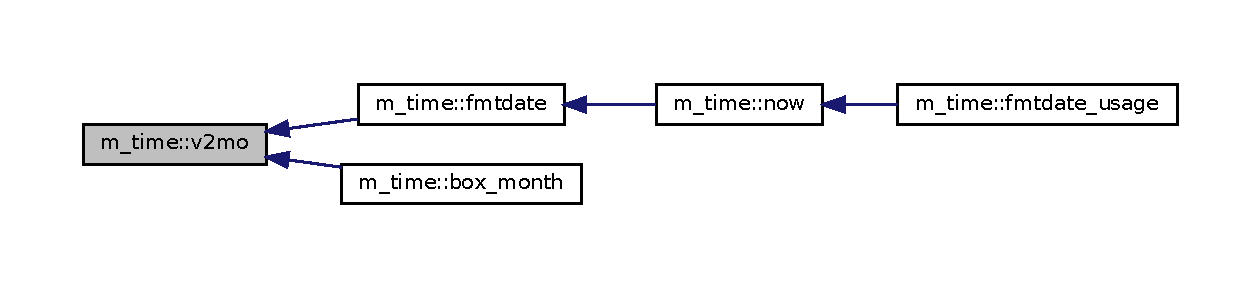
\includegraphics[width=350pt]{namespacem__time_a6f28cf00e4998bb50bb503f5e4bd3f77_icgraph}
\end{center}
\end{figure}
\mbox{\Hypertarget{namespacem__time_ac0ec48db8d508bfa23fe4b20c9d1c5a3}\label{namespacem__time_ac0ec48db8d508bfa23fe4b20c9d1c5a3}} 
\index{m\_time@{m\_time}!w2d@{w2d}}
\index{w2d@{w2d}!m\_time@{m\_time}}
\doxysubsubsection{\texorpdfstring{w2d()}{w2d()}}
{\footnotesize\ttfamily subroutine, public m\+\_\+time\+::w2d (\begin{DoxyParamCaption}\item[{integer, intent(in)}]{iso\+\_\+year,  }\item[{integer, intent(in)}]{iso\+\_\+week,  }\item[{integer, intent(in)}]{iso\+\_\+weekday,  }\item[{integer, dimension(8), intent(out)}]{dat }\end{DoxyParamCaption})}

\hypertarget{namespacem__time_autotoc_md136}{}\doxysubsubsection{N\+A\+ME}\label{namespacem__time_autotoc_md136}
w2d(3f) -\/ \mbox{[}M\+\_\+time\+:W\+E\+E\+K\+\_\+\+O\+F\+\_\+\+Y\+E\+AR\mbox{]} calculate D\+AT date-\/time array from iso-\/8601 Week-\/numbering year date yyyy-\/\+Www-\/d (L\+I\+C\+E\+N\+SE\+:PD)\hypertarget{namespacem__time_autotoc_md137}{}\doxysubsubsection{S\+Y\+N\+O\+P\+S\+IS}\label{namespacem__time_autotoc_md137}
\begin{DoxyVerb}subroutine w2d(iso_year,iso_week,iso_weekday,dat)

 integer,intent(in)      :: iso_year, iso_week, iso_weekday
 integer,intent(out)     :: dat(8)     ! output date array
\end{DoxyVerb}
\hypertarget{namespacem__time_autotoc_md138}{}\doxysubsubsection{D\+E\+S\+C\+R\+I\+P\+T\+I\+ON}\label{namespacem__time_autotoc_md138}
Given an I\+S\+O-\/8601 week return a \char`\"{}\+D\+A\+T\char`\"{} array defining a date and time, The I\+S\+O-\/8601 is supplied as three integer values defining the I\+SO year, week of year and weekday.\hypertarget{namespacem__time_autotoc_md139}{}\doxysubsubsection{O\+P\+T\+I\+O\+NS}\label{namespacem__time_autotoc_md139}
iso\+\_\+year I\+S\+O-\/8601 year number for the given date iso\+\_\+week I\+S\+O-\/8601 week number for the given date iso\+\_\+weekday I\+S\+O-\/8601 weekday number for the given date iso\+\_\+name I\+S\+O-\/8601 Week string for the data in the form \char`\"{}yyyy-\/\+Www-\/d\char`\"{}.\hypertarget{namespacem__time_autotoc_md140}{}\doxysubsubsection{R\+E\+T\+U\+R\+NS}\label{namespacem__time_autotoc_md140}
dat \char`\"{}\+D\+A\+T\char`\"{} array (an integer array of the same format as the array returned by the intrinsic D\+A\+T\+E\+\_\+\+A\+N\+D\+\_\+\+T\+I\+M\+E(3f)) describing the date to be used, which is the basic time description used by the other M\+\_\+time(3fm) module procedures.\hypertarget{namespacem__time_autotoc_md141}{}\doxysubsubsection{E\+X\+A\+M\+P\+LE}\label{namespacem__time_autotoc_md141}
Sample program\+:

program demo\+\_\+w2d use M\+\_\+time, only \+: w2d, fmtdate implicit none write($\ast$,\textquotesingle{}(a)\textquotesingle{})\& \& \textquotesingle{}Given Monday 29 December 2008 is written \char`\"{}2009-\/\+W01-\/1\char`\"{}\textquotesingle{} call printit(2009,1,1) write($\ast$,\textquotesingle{}(a)\textquotesingle{})\& \& \textquotesingle{}Given Sunday 3 January 2010 is written \char`\"{}2009-\/\+W53-\/7\char`\"{}\textquotesingle{} call printit(2009,53,7) write($\ast$,\textquotesingle{}(a)\textquotesingle{})\& \& \textquotesingle{}Given the Gregorian date Sun 31 December 2006 \& \&is written 2006-\/W52-\/7\textquotesingle{} call printit(2006,52,7) write($\ast$,\textquotesingle{}(a)\textquotesingle{})\& \& \textquotesingle{}Given 27 September 2008 is 2008-\/W39-\/6\textquotesingle{} call printit(2008,39,6) contains subroutine printit(iso\+\_\+year,iso\+\_\+week,iso\+\_\+weekday) ! I\+S\+O-\/8601 Week\+: 2016-\/W29-\/1 integer \+:: iso\+\_\+year, iso\+\_\+week, iso\+\_\+weekday ! input date array integer \+:: dat(8) call w2d(iso\+\_\+year,iso\+\_\+week,iso\+\_\+weekday,dat) write($\ast$,\textquotesingle{}(a,i0)\textquotesingle{})\textquotesingle{}G\+I\+V\+EN\+: \textquotesingle{} write($\ast$,\textquotesingle{}(a,i0)\textquotesingle{})\textquotesingle{}I\+S\+O-\/8601 year \textquotesingle{},iso\+\_\+year write($\ast$,\textquotesingle{}(a,i0)\textquotesingle{})\textquotesingle{}I\+S\+O-\/8601 week \textquotesingle{},iso\+\_\+week write($\ast$,\textquotesingle{}(a,i0)\textquotesingle{})\textquotesingle{}I\+S\+O-\/8601 weekday \textquotesingle{},iso\+\_\+weekday write($\ast$,\textquotesingle{}(a,i0)\textquotesingle{})\textquotesingle{}R\+E\+S\+U\+LT\+: \textquotesingle{} write($\ast$,\textquotesingle{}(a,$\ast$(i0\+:,\char`\"{},\char`\"{}))\textquotesingle{})\textquotesingle{} D\+AT array \textquotesingle{},dat write($\ast$,\textquotesingle{}(a,/,67(\char`\"{}=\char`\"{}))\textquotesingle{})\textquotesingle{} \textquotesingle{}//fmtdate(dat,\textquotesingle{}long\textquotesingle{}) end subroutine printit end program demo\+\_\+w2d

Results\+:

Given Monday 29 December 2008 is written \char`\"{}2009-\/\+W01-\/1\char`\"{} G\+I\+V\+EN\+: I\+S\+O-\/8601 year 2009 I\+S\+O-\/8601 week 1 I\+S\+O-\/8601 weekday 1 R\+E\+S\+U\+LT\+: D\+AT array 2008,12,29,-\/240,0,0,0,0 \hypertarget{namespacem__time_autotoc_md142}{}\doxysubsection{Monday, December 29th, 2008 12\+:00\+:00 A\+M U\+T\+C-\/04\+:00}\label{namespacem__time_autotoc_md142}
Given Sunday 3 January 2010 is written \char`\"{}2009-\/\+W53-\/7\char`\"{} G\+I\+V\+EN\+: I\+S\+O-\/8601 year 2009 I\+S\+O-\/8601 week 53 I\+S\+O-\/8601 weekday 7 R\+E\+S\+U\+LT\+: D\+AT array 2010,1,3,-\/240,0,0,0,0 \hypertarget{namespacem__time_autotoc_md143}{}\doxysubsection{Sunday, January 3rd, 2010 12\+:00\+:00 A\+M U\+T\+C-\/04\+:00}\label{namespacem__time_autotoc_md143}
Given the Gregorian date Sun 31 December 2006 is written 2006-\/W52-\/7 G\+I\+V\+EN\+: I\+S\+O-\/8601 year 2006 I\+S\+O-\/8601 week 52 I\+S\+O-\/8601 weekday 7 R\+E\+S\+U\+LT\+: D\+AT array 2006,12,31,-\/240,0,0,0,0 \hypertarget{namespacem__time_autotoc_md144}{}\doxysubsection{Sunday, December 31st, 2006 12\+:00\+:00 A\+M U\+T\+C-\/04\+:00}\label{namespacem__time_autotoc_md144}
Given 27 September 2008 is 2008-\/W39-\/6 G\+I\+V\+EN\+: I\+S\+O-\/8601 year 2008 I\+S\+O-\/8601 week 39 I\+S\+O-\/8601 weekday 6 R\+E\+S\+U\+LT\+: D\+AT array 2008,9,27,-\/240,0,0,0,0 \hypertarget{namespacem__time_autotoc_md145}{}\doxysubsection{Saturday, September 27th, 2008 12\+:00\+:00 A\+M U\+T\+C-\/04\+:00}\label{namespacem__time_autotoc_md145}
\hypertarget{namespacem__time_autotoc_md146}{}\doxysubsubsection{D\+E\+F\+I\+N\+I\+T\+I\+ON}\label{namespacem__time_autotoc_md146}
The I\+S\+O-\/8601 date and time standard was issued by the International Organization for Standardization (I\+SO). It is used (mainly) in government and business for fiscal years, as well as in timekeeping. The system specifies a week year atop the Gregorian calendar by defining a notation for ordinal weeks of the year.

An I\+SO week-\/numbering year (also called I\+SO year informally) has 52 or 53 full weeks. That is 364 or 371 days instead of the usual 365 or 366 days. The extra week is referred to here as a leap week, although I\+S\+O-\/8601 does not use this term. Weeks start with Monday. The first week of a year is the week that contains the first Thursday of the year (and, hence, always contains 4 January). I\+SO week year numbering therefore slightly deviates from the Gregorian for some days close to January 1st.\hypertarget{namespacem__time_autotoc_md147}{}\doxysubsubsection{M\+E\+T\+H\+OD}\label{namespacem__time_autotoc_md147}
Calculating a date given the year, week number and weekday

This method requires that one know the weekday of 4 January of the year in question. Add 3 to the number of this weekday, giving a correction to be used for dates within this year.

Method\+: Multiply the week number by 7, then add the weekday. From this sum subtract the correction for the year. The result is the ordinal date, which can be converted into a calendar date. If the ordinal date thus obtained is zero or negative, the date belongs to the previous calendar year; if greater than the number of days in the year, to the following year.

Example\+: year 2008, week 39, Saturday (day 6) Correction for 2008\+: 5 + 3 = 8 (39 x 7) + 6 = 279 279 -\/ 8 = 271 Ordinal day 271 of a leap year is day 271 -\/ 244 = 27 September Result\+: 27 September 2008\hypertarget{namespacem__time_autotoc_md148}{}\doxysubsubsection{I\+S\+O\+\_\+\+N\+A\+ME}\label{namespacem__time_autotoc_md148}
Week date representations are in the format Y\+Y\+Y\+Y\+Www-\/D.

o \mbox{[}Y\+Y\+YY\mbox{]} indicates the I\+SO week-\/numbering year which is slightly different from the traditional Gregorian calendar year. o \mbox{[}Www\mbox{]} is the week number prefixed by the letter W, from W01 through W53. o \mbox{[}D\mbox{]} is the weekday number, from 1 through 7, beginning with Monday and ending with Sunday.

For example, the Gregorian date 31 December 2006 corresponds to the Sunday of the 52nd week of 2006, and is written

2006-\/W52-\/7 (extended form) or 2006W527 (compact form).\hypertarget{namespacem__time_autotoc_md149}{}\doxysubsubsection{R\+E\+F\+E\+R\+E\+N\+CE}\label{namespacem__time_autotoc_md149}
From Wikipedia, the free encyclopedia 2016-\/08-\/08\hypertarget{namespacem__time_autotoc_md150}{}\doxysubsubsection{A\+U\+T\+H\+OR}\label{namespacem__time_autotoc_md150}
John S. Urban, 2015 \hypertarget{namespacem__time_autotoc_md151}{}\doxysubsubsection{L\+I\+C\+E\+N\+SE}\label{namespacem__time_autotoc_md151}
Public Domain 

References dow(), and o2d().

Here is the call graph for this function\+:\nopagebreak
\begin{figure}[H]
\begin{center}
\leavevmode
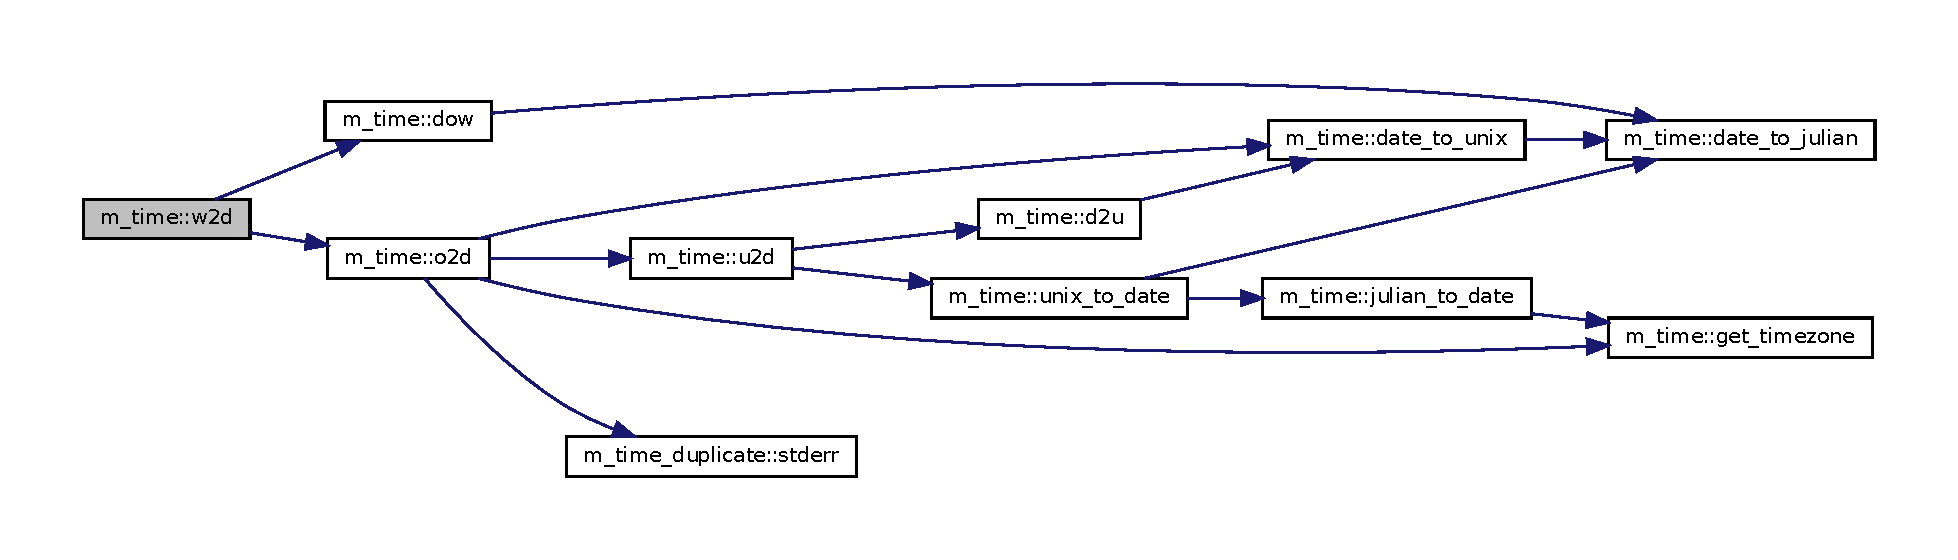
\includegraphics[width=350pt]{namespacem__time_ac0ec48db8d508bfa23fe4b20c9d1c5a3_cgraph}
\end{center}
\end{figure}


\doxysubsection{Variable Documentation}
\mbox{\Hypertarget{namespacem__time_a97725f8d657c24badff19a794f323a6b}\label{namespacem__time_a97725f8d657c24badff19a794f323a6b}} 
\index{m\_time@{m\_time}!dt\_day@{dt\_day}}
\index{dt\_day@{dt\_day}!m\_time@{m\_time}}
\doxysubsubsection{\texorpdfstring{dt\_day}{dt\_day}}
{\footnotesize\ttfamily real(kind=\mbox{\hyperlink{namespacem__time_ac10ea9e8d59ec74eaa7d89f2517d7422}{realtime}}), parameter, public m\+\_\+time\+::dt\+\_\+day =86400.\+0d0}

\mbox{\Hypertarget{namespacem__time_aa0ca2172092f5e7dcc9b8524e6516fd8}\label{namespacem__time_aa0ca2172092f5e7dcc9b8524e6516fd8}} 
\index{m\_time@{m\_time}!dt\_hour@{dt\_hour}}
\index{dt\_hour@{dt\_hour}!m\_time@{m\_time}}
\doxysubsubsection{\texorpdfstring{dt\_hour}{dt\_hour}}
{\footnotesize\ttfamily real(kind=\mbox{\hyperlink{namespacem__time_ac10ea9e8d59ec74eaa7d89f2517d7422}{realtime}}), parameter, public m\+\_\+time\+::dt\+\_\+hour =3600.\+0d0}

\mbox{\Hypertarget{namespacem__time_a9fe6fbb44e2779a2fcf96fba36c08918}\label{namespacem__time_a9fe6fbb44e2779a2fcf96fba36c08918}} 
\index{m\_time@{m\_time}!dt\_minute@{dt\_minute}}
\index{dt\_minute@{dt\_minute}!m\_time@{m\_time}}
\doxysubsubsection{\texorpdfstring{dt\_minute}{dt\_minute}}
{\footnotesize\ttfamily real(kind=\mbox{\hyperlink{namespacem__time_ac10ea9e8d59ec74eaa7d89f2517d7422}{realtime}}), parameter, public m\+\_\+time\+::dt\+\_\+minute =60.\+0d0}

\mbox{\Hypertarget{namespacem__time_a3d53519e90264faccdae67e389ffc003}\label{namespacem__time_a3d53519e90264faccdae67e389ffc003}} 
\index{m\_time@{m\_time}!dt\_week@{dt\_week}}
\index{dt\_week@{dt\_week}!m\_time@{m\_time}}
\doxysubsubsection{\texorpdfstring{dt\_week}{dt\_week}}
{\footnotesize\ttfamily real(kind=\mbox{\hyperlink{namespacem__time_ac10ea9e8d59ec74eaa7d89f2517d7422}{realtime}}), parameter, public m\+\_\+time\+::dt\+\_\+week =\mbox{\hyperlink{namespacem__time_a97725f8d657c24badff19a794f323a6b}{dt\+\_\+day}}$\ast$7.\+0d0}

\mbox{\Hypertarget{namespacem__time_ac10ea9e8d59ec74eaa7d89f2517d7422}\label{namespacem__time_ac10ea9e8d59ec74eaa7d89f2517d7422}} 
\index{m\_time@{m\_time}!realtime@{realtime}}
\index{realtime@{realtime}!m\_time@{m\_time}}
\doxysubsubsection{\texorpdfstring{realtime}{realtime}}
{\footnotesize\ttfamily integer, parameter, public m\+\_\+time\+::realtime =kind(0.\+0d0)}

\mbox{\Hypertarget{namespacem__time_a48130b5a95a3f2e776269dcee1426797}\label{namespacem__time_a48130b5a95a3f2e776269dcee1426797}} 
\index{m\_time@{m\_time}!secday@{secday}}
\index{secday@{secday}!m\_time@{m\_time}}
\doxysubsubsection{\texorpdfstring{secday}{secday}}
{\footnotesize\ttfamily real(kind=\mbox{\hyperlink{namespacem__time_ac10ea9e8d59ec74eaa7d89f2517d7422}{realtime}}), parameter, private m\+\_\+time\+::secday =86400.\+0d0\hspace{0.3cm}{\ttfamily [private]}}


\hypertarget{namespacem__time__duplicate}{}\doxysection{m\+\_\+time\+\_\+duplicate Module Reference}
\label{namespacem__time__duplicate}\index{m\_time\_duplicate@{m\_time\_duplicate}}
\doxysubsection*{Data Types}
\begin{DoxyCompactItemize}
\item 
interface \mbox{\hyperlink{interfacem__time__duplicate_1_1string__to__value}{string\+\_\+to\+\_\+value}}
\item 
interface \mbox{\hyperlink{interfacem__time__duplicate_1_1v2s}{v2s}}
\end{DoxyCompactItemize}
\doxysubsection*{Functions/\+Subroutines}
\begin{DoxyCompactItemize}
\item 
subroutine, public \mbox{\hyperlink{namespacem__time__duplicate_abc203f3a6afc1edeecbcdc58b187a5d5}{substitute}} (targetline, old, new, ierr, start, end)
\item 
elemental pure character(len(str)) function, public \mbox{\hyperlink{namespacem__time__duplicate_aabdd1a3e01b26e896bd06aee488de7c6}{upper}} (str, begin, end)
\item 
elemental pure character(len(str)) function, public \mbox{\hyperlink{namespacem__time__duplicate_af8b4555e0c47e2ec327f0434d84b9c56}{lower}} (str, begin, end)
\item 
subroutine \mbox{\hyperlink{namespacem__time__duplicate_aaf5c25d7bce4f2776df6c1e586b2e277}{stderr}} (string)
\item 
pure character(len=\+:) function, allocatable, public \mbox{\hyperlink{namespacem__time__duplicate_a487dbbb116d2c7022b39869d4990cf6f}{adjustc}} (string, length)
\item 
character(len=len(str)) function, public \mbox{\hyperlink{namespacem__time__duplicate_a20fc022f66383c65302e990c00432f38}{compact}} (str, char)
\item 
doubleprecision function, public \mbox{\hyperlink{namespacem__time__duplicate_a118f0d70fa6f319fbd773008c7f86ef9}{s2v}} (chars, ierr, onerr)
\item 
subroutine, public \mbox{\hyperlink{namespacem__time__duplicate_a326e0d62d92969a231864997eea2ab98}{split}} (input\+\_\+line, array, delimiters, order, nulls)
\item 
subroutine, public \mbox{\hyperlink{namespacem__time__duplicate_a1bfa9e4483f2452c89c0388971bb21bd}{string\+\_\+to\+\_\+values}} (line, iread, values, inums, delims, ierr)
\item 
pure character(len=len(instr)) function, public \mbox{\hyperlink{namespacem__time__duplicate_ac8388a45881cf7c2f9047b4d643ed3f2}{transliterate}} (instr, old\+\_\+set, new\+\_\+set)
\item 
character(len=\+:) function, allocatable \mbox{\hyperlink{namespacem__time__duplicate_a84f53c1e0d6c1c9fe70b19549921d14b}{d2s}} (dvalue, fmt)
\item 
character(len=\+:) function, allocatable \mbox{\hyperlink{namespacem__time__duplicate_a9d1f96975ddf101c13c2f7f0dbf92a02}{r2s}} (rvalue, fmt)
\item 
character(len=\+:) function, allocatable \mbox{\hyperlink{namespacem__time__duplicate_a7570c5a3b71c4ea4f376a38b285ccbd8}{i2s}} (ivalue, fmt)
\item 
character(len=\+:) function, allocatable \mbox{\hyperlink{namespacem__time__duplicate_a4bd5e96c3ed16383c576c4e362c16b82}{l2s}} (lvalue, fmt)
\item 
subroutine \mbox{\hyperlink{namespacem__time__duplicate_ab836a3b7c441e5b324639db734b7de9f}{value\+\_\+to\+\_\+string}} (gval, chars, length, err, fmt, trimz)
\item 
subroutine \mbox{\hyperlink{namespacem__time__duplicate_ae5ec641c9bdaa5d9377e47310e2165be}{trimzeros}} (string)
\item 
subroutine \mbox{\hyperlink{namespacem__time__duplicate_a9e2a87974ffb9b81dcfb0ecee076180f}{a2r}} (chars, valu, ierr)
\item 
subroutine \mbox{\hyperlink{namespacem__time__duplicate_aaf8891d2fdbd165fecbdf78335f926fc}{a2i}} (chars, valu, ierr)
\item 
subroutine \mbox{\hyperlink{namespacem__time__duplicate_ab86bb390cc56184faeef5543735eecc4}{a2d}} (chars, valu, ierr, onerr)
\item 
logical function \mbox{\hyperlink{namespacem__time__duplicate_a66a83a4b3d6324843c984658784b2c4e}{decodebase}} (string, basein, out\+\_\+baseten)
\end{DoxyCompactItemize}


\doxysubsection{Function/\+Subroutine Documentation}
\mbox{\Hypertarget{namespacem__time__duplicate_ab86bb390cc56184faeef5543735eecc4}\label{namespacem__time__duplicate_ab86bb390cc56184faeef5543735eecc4}} 
\index{m\_time\_duplicate@{m\_time\_duplicate}!a2d@{a2d}}
\index{a2d@{a2d}!m\_time\_duplicate@{m\_time\_duplicate}}
\doxysubsubsection{\texorpdfstring{a2d()}{a2d()}}
{\footnotesize\ttfamily subroutine m\+\_\+time\+\_\+duplicate\+::a2d (\begin{DoxyParamCaption}\item[{character(len=$\ast$), intent(in)}]{chars,  }\item[{doubleprecision, intent(out)}]{valu,  }\item[{integer, intent(out)}]{ierr,  }\item[{class($\ast$), intent(in), optional}]{onerr }\end{DoxyParamCaption})}



References decodebase(), stderr(), and substitute().

Here is the call graph for this function\+:\nopagebreak
\begin{figure}[H]
\begin{center}
\leavevmode
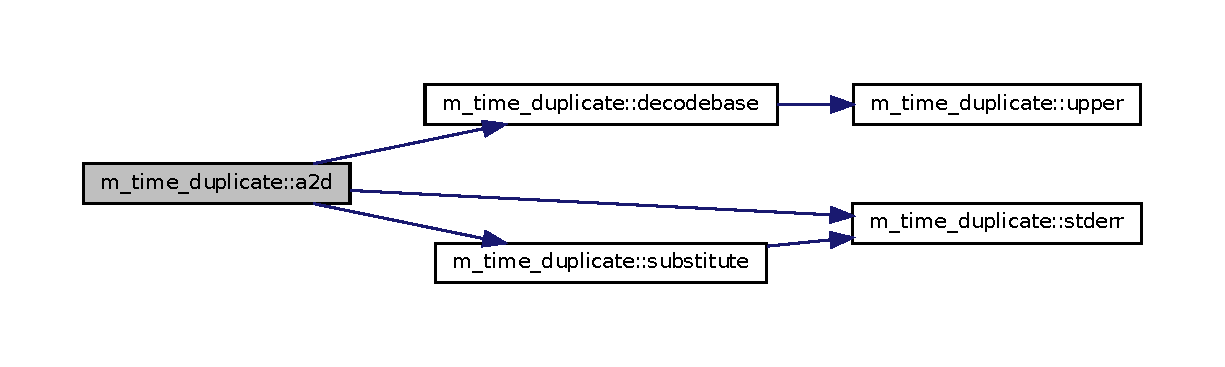
\includegraphics[width=350pt]{namespacem__time__duplicate_ab86bb390cc56184faeef5543735eecc4_cgraph}
\end{center}
\end{figure}
Here is the caller graph for this function\+:\nopagebreak
\begin{figure}[H]
\begin{center}
\leavevmode
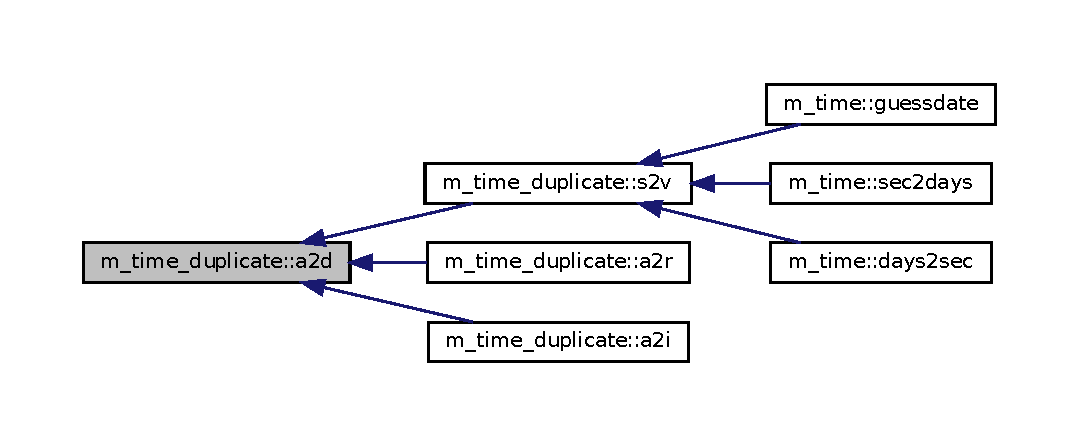
\includegraphics[width=350pt]{namespacem__time__duplicate_ab86bb390cc56184faeef5543735eecc4_icgraph}
\end{center}
\end{figure}
\mbox{\Hypertarget{namespacem__time__duplicate_aaf8891d2fdbd165fecbdf78335f926fc}\label{namespacem__time__duplicate_aaf8891d2fdbd165fecbdf78335f926fc}} 
\index{m\_time\_duplicate@{m\_time\_duplicate}!a2i@{a2i}}
\index{a2i@{a2i}!m\_time\_duplicate@{m\_time\_duplicate}}
\doxysubsubsection{\texorpdfstring{a2i()}{a2i()}}
{\footnotesize\ttfamily subroutine m\+\_\+time\+\_\+duplicate\+::a2i (\begin{DoxyParamCaption}\item[{character(len=$\ast$), intent(in)}]{chars,  }\item[{integer, intent(out)}]{valu,  }\item[{integer, intent(out)}]{ierr }\end{DoxyParamCaption})}



References a2d(), and stderr().

Here is the call graph for this function\+:\nopagebreak
\begin{figure}[H]
\begin{center}
\leavevmode
\includegraphics[width=350pt]{namespacem__time__duplicate_aaf8891d2fdbd165fecbdf78335f926fc_cgraph}
\end{center}
\end{figure}
\mbox{\Hypertarget{namespacem__time__duplicate_a9e2a87974ffb9b81dcfb0ecee076180f}\label{namespacem__time__duplicate_a9e2a87974ffb9b81dcfb0ecee076180f}} 
\index{m\_time\_duplicate@{m\_time\_duplicate}!a2r@{a2r}}
\index{a2r@{a2r}!m\_time\_duplicate@{m\_time\_duplicate}}
\doxysubsubsection{\texorpdfstring{a2r()}{a2r()}}
{\footnotesize\ttfamily subroutine m\+\_\+time\+\_\+duplicate\+::a2r (\begin{DoxyParamCaption}\item[{character(len=$\ast$), intent(in)}]{chars,  }\item[{real, intent(out)}]{valu,  }\item[{integer, intent(out)}]{ierr }\end{DoxyParamCaption})}

\hypertarget{namespacem__time__duplicate_autotoc_md334}{}\doxysubsubsection{N\+A\+ME}\label{namespacem__time__duplicate_autotoc_md334}
string\+\_\+to\+\_\+value(3f) -\/ \mbox{[}M\+\_\+strings\+:N\+U\+M\+E\+R\+IC\mbox{]} subroutine returns numeric value from string (L\+I\+C\+E\+N\+SE\+:PD)\hypertarget{namespacem__time__duplicate_autotoc_md335}{}\doxysubsubsection{S\+Y\+N\+O\+P\+S\+IS}\label{namespacem__time__duplicate_autotoc_md335}
\begin{DoxyVerb}subroutine string_to_value(chars,valu,ierr)

 character(len=*),intent(in)              :: chars   ! input string
 integer|real|doubleprecision,intent(out) :: valu
 integer,intent(out)                      :: ierr
\end{DoxyVerb}
 \hypertarget{namespacem__time__duplicate_autotoc_md336}{}\doxysubsubsection{D\+E\+S\+C\+R\+I\+P\+T\+I\+ON}\label{namespacem__time__duplicate_autotoc_md336}
returns a numeric value from a numeric character string.

works with any g-\/format input, including integer, real, and exponential. If the input string begins with \char`\"{}\+B\char`\"{}, \char`\"{}\+Z\char`\"{}, or \char`\"{}\+O\char`\"{} and otherwise represents a positive whole number it is assumed to be a binary, hexadecimal, or octal value. If the string contains commas they are removed. If the string is of the form NN\+:M\+MM... or N\+N\+::\+M\+MM then NN is assumed to be the base of the whole number.

if an error occurs in the R\+E\+AD, I\+O\+S\+T\+AT is returned in I\+E\+RR and value is set to zero. if no error occurs, I\+E\+RR=0. \hypertarget{namespacem__time__duplicate_autotoc_md337}{}\doxysubsubsection{O\+P\+T\+I\+O\+NS}\label{namespacem__time__duplicate_autotoc_md337}
C\+H\+A\+RS input string to read numeric value from \hypertarget{namespacem__time__duplicate_autotoc_md338}{}\doxysubsubsection{R\+E\+T\+U\+R\+NS}\label{namespacem__time__duplicate_autotoc_md338}
V\+A\+LU numeric value returned. May be I\+N\+T\+E\+G\+ER, R\+E\+AL, or D\+O\+U\+B\+L\+E\+P\+R\+E\+C\+I\+S\+I\+ON. I\+E\+RR error flag (0 == no error) \hypertarget{namespacem__time__duplicate_autotoc_md339}{}\doxysubsubsection{E\+X\+A\+M\+P\+LE}\label{namespacem__time__duplicate_autotoc_md339}
\begin{DoxyVerb}Sample Program:

 program demo_string_to_value
 use M_strings, only: string_to_value
 character(len=80) :: string
    string=' -40.5e-2 '
    call string_to_value(string,value,ierr)
    write(*,*) 'value of string ['//trim(string)//'] is ',value
 end program demo_string_to_value
\end{DoxyVerb}
 \hypertarget{namespacem__time__duplicate_autotoc_md340}{}\doxysubsubsection{A\+U\+T\+H\+OR}\label{namespacem__time__duplicate_autotoc_md340}
John S. Urban \hypertarget{namespacem__time__duplicate_autotoc_md341}{}\doxysubsubsection{L\+I\+C\+E\+N\+SE}\label{namespacem__time__duplicate_autotoc_md341}
Public Domain 

References a2d(), and stderr().

Here is the call graph for this function\+:\nopagebreak
\begin{figure}[H]
\begin{center}
\leavevmode
\includegraphics[width=350pt]{namespacem__time__duplicate_a9e2a87974ffb9b81dcfb0ecee076180f_cgraph}
\end{center}
\end{figure}
\mbox{\Hypertarget{namespacem__time__duplicate_a487dbbb116d2c7022b39869d4990cf6f}\label{namespacem__time__duplicate_a487dbbb116d2c7022b39869d4990cf6f}} 
\index{m\_time\_duplicate@{m\_time\_duplicate}!adjustc@{adjustc}}
\index{adjustc@{adjustc}!m\_time\_duplicate@{m\_time\_duplicate}}
\doxysubsubsection{\texorpdfstring{adjustc()}{adjustc()}}
{\footnotesize\ttfamily pure character(len=\+:) function, allocatable, public m\+\_\+time\+\_\+duplicate\+::adjustc (\begin{DoxyParamCaption}\item[{character(len=$\ast$), intent(in)}]{string,  }\item[{integer, intent(in), optional}]{length }\end{DoxyParamCaption})}

\hypertarget{namespacem__time__duplicate_autotoc_md260}{}\doxysubsubsection{N\+A\+ME}\label{namespacem__time__duplicate_autotoc_md260}
adjustc(3f) -\/ \mbox{[}M\+\_\+strings\+:W\+H\+I\+T\+E\+S\+P\+A\+CE\mbox{]} center text (L\+I\+C\+E\+N\+SE\+:PD)\hypertarget{namespacem__time__duplicate_autotoc_md261}{}\doxysubsubsection{S\+Y\+N\+O\+P\+S\+IS}\label{namespacem__time__duplicate_autotoc_md261}
pure function adjustc(string\mbox{[},length\mbox{]})

character(len=$\ast$),intent(in) \+:: string integer,intent(in),optional \+:: length character(len=\+:),allocatable \+:: adjustc \hypertarget{namespacem__time__duplicate_autotoc_md262}{}\doxysubsubsection{D\+E\+S\+C\+R\+I\+P\+T\+I\+ON}\label{namespacem__time__duplicate_autotoc_md262}
Centers input text in a string of the length specified. Returns a string of length L\+E\+N\+G\+TH if L\+E\+N\+G\+TH is present. Otherwise returns a string of the length of the input string. \hypertarget{namespacem__time__duplicate_autotoc_md263}{}\doxysubsubsection{O\+P\+T\+I\+O\+NS}\label{namespacem__time__duplicate_autotoc_md263}
string input string to trim and center length line length to center text in, optional. \hypertarget{namespacem__time__duplicate_autotoc_md264}{}\doxysubsubsection{R\+E\+T\+U\+R\+NS}\label{namespacem__time__duplicate_autotoc_md264}
adjustc centered output string\hypertarget{namespacem__time__duplicate_autotoc_md265}{}\doxysubsubsection{E\+X\+A\+M\+P\+L\+ES}\label{namespacem__time__duplicate_autotoc_md265}
\begin{DoxyVerb}Sample Program:

 program demo_adjustc
 use M_strings, only : adjustc
 !  using length of the input string
    write(*,'(a)')       '================================'
    write(*,'(a)')adjustc('centered string                 ')
    write(*,'(a)')adjustc('                 centered string')
    write(*,'(a)')adjustc('  centered string               ')
 !  using explicit output string length
    write(*,'(a)')repeat('=',50)
    write(*,'(a)')adjustc('this is a centered string',50)
    write(*,'(a)')repeat('=',50)
 end program demo_adjustc

Expected output:

 \================================
         centered string
         centered string
         centered string
 \==================================================
             this is a centered string
 \==================================================
\end{DoxyVerb}
 \hypertarget{namespacem__time__duplicate_autotoc_md266}{}\doxysubsubsection{A\+U\+T\+H\+OR}\label{namespacem__time__duplicate_autotoc_md266}
John S. Urban \hypertarget{namespacem__time__duplicate_autotoc_md267}{}\doxysubsubsection{L\+I\+C\+E\+N\+SE}\label{namespacem__time__duplicate_autotoc_md267}
Public Domain
\begin{DoxyParams}[1]{Parameters}
\mbox{\texttt{ in}}  & {\em string} & P\+R\+O\+C\+E\+D\+U\+RE adjustc(3f) D\+E\+S\+C\+R\+I\+P\+T\+I\+ON center text using implicit or explicit length \\
\hline
\end{DoxyParams}
\hypertarget{namespacem__time__duplicate_autotoc_md269}{}\doxysubsubsection{V\+E\+R\+S\+I\+O\+N     2.\+0, 20160711}\label{namespacem__time__duplicate_autotoc_md269}
A\+U\+T\+H\+OR John S. Urban Here is the caller graph for this function\+:\nopagebreak
\begin{figure}[H]
\begin{center}
\leavevmode
\includegraphics[width=350pt]{namespacem__time__duplicate_a487dbbb116d2c7022b39869d4990cf6f_icgraph}
\end{center}
\end{figure}
\mbox{\Hypertarget{namespacem__time__duplicate_a20fc022f66383c65302e990c00432f38}\label{namespacem__time__duplicate_a20fc022f66383c65302e990c00432f38}} 
\index{m\_time\_duplicate@{m\_time\_duplicate}!compact@{compact}}
\index{compact@{compact}!m\_time\_duplicate@{m\_time\_duplicate}}
\doxysubsubsection{\texorpdfstring{compact()}{compact()}}
{\footnotesize\ttfamily character(len=len(str)) function, public m\+\_\+time\+\_\+duplicate\+::compact (\begin{DoxyParamCaption}\item[{character(len=$\ast$), intent(in)}]{str,  }\item[{character(len=$\ast$), intent(in), optional}]{char }\end{DoxyParamCaption})}

\hypertarget{namespacem__time__duplicate_autotoc_md270}{}\doxysubsubsection{N\+A\+ME}\label{namespacem__time__duplicate_autotoc_md270}
compact(3f) -\/ \mbox{[}M\+\_\+strings\+:W\+H\+I\+T\+E\+S\+P\+A\+CE\mbox{]} converts contiguous whitespace to a single character (or nothing) (L\+I\+C\+E\+N\+SE\+:PD)\hypertarget{namespacem__time__duplicate_autotoc_md271}{}\doxysubsubsection{S\+Y\+N\+O\+P\+S\+IS}\label{namespacem__time__duplicate_autotoc_md271}
\begin{DoxyVerb}function compact(STR,CHAR) result (OUTSTR)

 character(len=*),intent(in)          :: STR
 character(len=*),intent(in),optional :: CHAR
 character(len=len(str))              :: OUTSTR
\end{DoxyVerb}
 \hypertarget{namespacem__time__duplicate_autotoc_md272}{}\doxysubsubsection{D\+E\+S\+C\+R\+I\+P\+T\+I\+ON}\label{namespacem__time__duplicate_autotoc_md272}
C\+O\+M\+P\+A\+C\+T(3f) converts multiple spaces, tabs and control characters (called \char`\"{}whitespace\char`\"{}) to a single character or nothing. Leading whitespace is removed.\hypertarget{namespacem__time__duplicate_autotoc_md273}{}\doxysubsubsection{O\+P\+T\+I\+O\+NS}\label{namespacem__time__duplicate_autotoc_md273}
S\+TR input string to reduce or remove whitespace from C\+H\+AR By default the character that replaces adjacent whitespace is a space. If the optional C\+H\+AR parameter is supplied it will be used to replace the whitespace. If a null character is supplied for C\+H\+AR whitespace is removed. \hypertarget{namespacem__time__duplicate_autotoc_md274}{}\doxysubsubsection{R\+E\+T\+U\+R\+NS}\label{namespacem__time__duplicate_autotoc_md274}
O\+U\+T\+S\+TR string of same length as input string but with all contiguous whitespace reduced to a single space and leading whitespace removed\hypertarget{namespacem__time__duplicate_autotoc_md275}{}\doxysubsubsection{E\+X\+A\+M\+P\+L\+ES}\label{namespacem__time__duplicate_autotoc_md275}
\begin{DoxyVerb}Sample Program:

 program demo_compact
 use M_strings, only : compact
 implicit none
 ! produces 'This is a test               '
 write(*,*)compact('  This     is      a     test  ')
 ! produces 'Thisisatest                  '
 write(*,*)compact('  This     is      a     test  ',char='')
 ! produces 'This:is:a:test               '
 write(*,*)compact('  This     is      a     test  ',char=':')
 ! note CHAR is used to replace the whitespace, but if CHAR is
 ! in the original string it is just copied
 write(*,*)compact('A  AA    A   AAAAA',char='A')
 ! produces (original A characters are left as-is) 'AAAAAAAAAAAA'
 ! not 'A'
 end program demo_compact

Expected output

 >This is a test
 >Thisisatest
 >This:is:a:test
 >AAAAAAAAAAAA
\end{DoxyVerb}
 \hypertarget{namespacem__time__duplicate_autotoc_md276}{}\doxysubsubsection{A\+U\+T\+H\+OR}\label{namespacem__time__duplicate_autotoc_md276}
John S. Urban \hypertarget{namespacem__time__duplicate_autotoc_md277}{}\doxysubsubsection{L\+I\+C\+E\+N\+SE}\label{namespacem__time__duplicate_autotoc_md277}
Public Domain Here is the caller graph for this function\+:\nopagebreak
\begin{figure}[H]
\begin{center}
\leavevmode
\includegraphics[width=350pt]{namespacem__time__duplicate_a20fc022f66383c65302e990c00432f38_icgraph}
\end{center}
\end{figure}
\mbox{\Hypertarget{namespacem__time__duplicate_a84f53c1e0d6c1c9fe70b19549921d14b}\label{namespacem__time__duplicate_a84f53c1e0d6c1c9fe70b19549921d14b}} 
\index{m\_time\_duplicate@{m\_time\_duplicate}!d2s@{d2s}}
\index{d2s@{d2s}!m\_time\_duplicate@{m\_time\_duplicate}}
\doxysubsubsection{\texorpdfstring{d2s()}{d2s()}}
{\footnotesize\ttfamily character(len=\+:) function, allocatable m\+\_\+time\+\_\+duplicate\+::d2s (\begin{DoxyParamCaption}\item[{doubleprecision, intent(in)}]{dvalue,  }\item[{character(len=$\ast$), intent(in), optional}]{fmt }\end{DoxyParamCaption})}

\hypertarget{namespacem__time__duplicate_autotoc_md311}{}\doxysubsubsection{N\+A\+ME}\label{namespacem__time__duplicate_autotoc_md311}
v2s(3f) -\/ \mbox{[}M\+\_\+strings\+:N\+U\+M\+E\+R\+IC\mbox{]} return numeric string from a numeric value (L\+I\+C\+E\+N\+SE\+:PD)\hypertarget{namespacem__time__duplicate_autotoc_md312}{}\doxysubsubsection{S\+Y\+N\+O\+P\+S\+IS}\label{namespacem__time__duplicate_autotoc_md312}
\begin{DoxyVerb}   function v2s(value) result(outstr)

    integer|real|doubleprecision|logical,intent(in ) :: value
    character(len=:),allocatable :: outstr
    character(len=*),optional,intent(in) :: fmt
\end{DoxyVerb}
\hypertarget{namespacem__time__duplicate_autotoc_md313}{}\doxysubsubsection{D\+E\+S\+C\+R\+I\+P\+T\+I\+ON}\label{namespacem__time__duplicate_autotoc_md313}
v2s(3f) returns a representation of a numeric value as a string when given a numeric value of type R\+E\+AL, D\+O\+U\+B\+L\+E\+P\+R\+E\+C\+I\+S\+I\+ON, I\+N\+T\+E\+G\+ER or L\+O\+G\+I\+C\+AL. It creates the strings using internal W\+R\+I\+T\+E() statements. Trailing zeros are removed from non-\/zero values, and the string is left-\/justified.\hypertarget{namespacem__time__duplicate_autotoc_md314}{}\doxysubsubsection{O\+P\+T\+I\+O\+NS}\label{namespacem__time__duplicate_autotoc_md314}
V\+A\+L\+UE input value to be converted to a string F\+MT format can be explicitly given, but is limited to generating a string of eighty or less characters.\hypertarget{namespacem__time__duplicate_autotoc_md315}{}\doxysubsubsection{R\+E\+T\+U\+R\+NS}\label{namespacem__time__duplicate_autotoc_md315}
O\+U\+T\+S\+TR returned string representing input value,\hypertarget{namespacem__time__duplicate_autotoc_md316}{}\doxysubsubsection{E\+X\+A\+M\+P\+LE}\label{namespacem__time__duplicate_autotoc_md316}
\begin{DoxyVerb}Sample Program:

 program demo_v2s
 use M_strings, only: v2s
 write(*,*) 'The value of 3.0/4.0 is ['//v2s(3.0/4.0)//']'
 write(*,*) 'The value of 1234    is ['//v2s(1234)//']'
 write(*,*) 'The value of 0d0     is ['//v2s(0d0)//']'
 write(*,*) 'The value of .false. is ['//v2s(.false.)//']'
 write(*,*) 'The value of .true. is  ['//v2s(.true.)//']'
 end program demo_v2s

Expected output

 The value of 3.0/4.0 is [0.75]
 The value of 1234    is [1234]
 The value of 0d0     is [0]
 The value of .false. is [F]
 The value of .true. is  [T]
\end{DoxyVerb}
\hypertarget{namespacem__time__duplicate_autotoc_md317}{}\doxysubsubsection{A\+U\+T\+H\+OR}\label{namespacem__time__duplicate_autotoc_md317}
John S. Urban \hypertarget{namespacem__time__duplicate_autotoc_md318}{}\doxysubsubsection{L\+I\+C\+E\+N\+SE}\label{namespacem__time__duplicate_autotoc_md318}
Public Domain 

References value\+\_\+to\+\_\+string().

Here is the call graph for this function\+:\nopagebreak
\begin{figure}[H]
\begin{center}
\leavevmode
\includegraphics[width=350pt]{namespacem__time__duplicate_a84f53c1e0d6c1c9fe70b19549921d14b_cgraph}
\end{center}
\end{figure}
\mbox{\Hypertarget{namespacem__time__duplicate_a66a83a4b3d6324843c984658784b2c4e}\label{namespacem__time__duplicate_a66a83a4b3d6324843c984658784b2c4e}} 
\index{m\_time\_duplicate@{m\_time\_duplicate}!decodebase@{decodebase}}
\index{decodebase@{decodebase}!m\_time\_duplicate@{m\_time\_duplicate}}
\doxysubsubsection{\texorpdfstring{decodebase()}{decodebase()}}
{\footnotesize\ttfamily logical function m\+\_\+time\+\_\+duplicate\+::decodebase (\begin{DoxyParamCaption}\item[{character(len=$\ast$), intent(in)}]{string,  }\item[{integer, intent(in)}]{basein,  }\item[{integer, intent(out)}]{out\+\_\+baseten }\end{DoxyParamCaption})}

\hypertarget{namespacem__time__duplicate_autotoc_md342}{}\doxysubsubsection{N\+A\+ME}\label{namespacem__time__duplicate_autotoc_md342}
decodebase(3f) -\/ \mbox{[}M\+\_\+strings\+:B\+A\+SE\mbox{]} convert whole number string in base \mbox{[}2-\/36\mbox{]} to base 10 number (L\+I\+C\+E\+N\+SE\+:PD)\hypertarget{namespacem__time__duplicate_autotoc_md343}{}\doxysubsubsection{S\+Y\+N\+O\+P\+S\+IS}\label{namespacem__time__duplicate_autotoc_md343}
\begin{DoxyVerb}logical function decodebase(string,basein,out10)

 character(len=*),intent(in)  :: string
 integer,intent(in)           :: basein
 integer,intent(out)          :: out10
\end{DoxyVerb}
 \hypertarget{namespacem__time__duplicate_autotoc_md344}{}\doxysubsubsection{D\+E\+S\+C\+R\+I\+P\+T\+I\+ON}\label{namespacem__time__duplicate_autotoc_md344}
Convert a numeric string representing a whole number in base B\+A\+S\+E\+IN to base 10. The function returns F\+A\+L\+SE if B\+A\+S\+E\+IN is not in the range \mbox{[}2..36\mbox{]} or if string S\+T\+R\+I\+NG contains invalid characters in base B\+A\+S\+E\+IN or if result O\+U\+T10 is too big

The letters A,B,...,Z represent 10,11,...,36 in the base $>$ 10.\hypertarget{namespacem__time__duplicate_autotoc_md345}{}\doxysubsubsection{O\+P\+T\+I\+O\+NS}\label{namespacem__time__duplicate_autotoc_md345}
string input string. It represents a whole number in the base specified by B\+A\+S\+E\+IN unless B\+A\+S\+E\+IN is set to zero. When B\+A\+S\+E\+IN is zero S\+T\+R\+I\+NG is assumed to be of the form B\+A\+S\+E\+::\+V\+A\+L\+UE where B\+A\+SE represents the function normally provided by B\+A\+S\+E\+IN. basein base of input string; either 0 or from 2 to 36. out10 output value in base 10\hypertarget{namespacem__time__duplicate_autotoc_md346}{}\doxysubsubsection{E\+X\+A\+M\+P\+LE}\label{namespacem__time__duplicate_autotoc_md346}
\begin{DoxyVerb}Sample program:

 program demo_decodebase
 use M_strings, only : codebase, decodebase
 implicit none
 integer           :: ba,bd
 character(len=40) :: x,y
 integer           :: r

 print *,' BASE CONVERSION'
 write(*,'("Start   Base (2 to 36): ")',advance='no'); read *, bd
 write(*,'("Arrival Base (2 to 36): ")',advance='no'); read *, ba
 INFINITE: do
    print *,''
    write(*,'("Enter number in start base: ")',advance='no'); read *, x
    if(x.eq.'0') exit INFINITE
    if(decodebase(x,bd,r)) then
       if(codebase(r,ba,y)) then
         write(*,'("In base ",I2,": ",A20)')  ba, y
       else
         print *,'Error in coding number.'
       endif
    else
       print *,'Error in decoding number.'
    endif
 enddo INFINITE

 end program demo_decodebase
\end{DoxyVerb}
\hypertarget{namespacem__time__duplicate_autotoc_md347}{}\doxysubsubsection{A\+U\+T\+H\+OR}\label{namespacem__time__duplicate_autotoc_md347}
John S. Urban

Ref.\+: "Math matiques en Turbo-\/\+Pascal by M. Ducamp and A. Reverchon (2), Eyrolles, Paris, 1988".

based on a F90 Version By J-\/P Moreau (www.\+jpmoreau.\+fr)\hypertarget{namespacem__time__duplicate_autotoc_md348}{}\doxysubsubsection{L\+I\+C\+E\+N\+SE}\label{namespacem__time__duplicate_autotoc_md348}
Public Domain 

References upper().

Here is the call graph for this function\+:\nopagebreak
\begin{figure}[H]
\begin{center}
\leavevmode
\includegraphics[width=350pt]{namespacem__time__duplicate_a66a83a4b3d6324843c984658784b2c4e_cgraph}
\end{center}
\end{figure}
Here is the caller graph for this function\+:\nopagebreak
\begin{figure}[H]
\begin{center}
\leavevmode
\includegraphics[width=350pt]{namespacem__time__duplicate_a66a83a4b3d6324843c984658784b2c4e_icgraph}
\end{center}
\end{figure}
\mbox{\Hypertarget{namespacem__time__duplicate_a7570c5a3b71c4ea4f376a38b285ccbd8}\label{namespacem__time__duplicate_a7570c5a3b71c4ea4f376a38b285ccbd8}} 
\index{m\_time\_duplicate@{m\_time\_duplicate}!i2s@{i2s}}
\index{i2s@{i2s}!m\_time\_duplicate@{m\_time\_duplicate}}
\doxysubsubsection{\texorpdfstring{i2s()}{i2s()}}
{\footnotesize\ttfamily character(len=\+:) function, allocatable m\+\_\+time\+\_\+duplicate\+::i2s (\begin{DoxyParamCaption}\item[{integer, intent(in)}]{ivalue,  }\item[{character(len=$\ast$), intent(in), optional}]{fmt }\end{DoxyParamCaption})}



References value\+\_\+to\+\_\+string().

Here is the call graph for this function\+:\nopagebreak
\begin{figure}[H]
\begin{center}
\leavevmode
\includegraphics[width=350pt]{namespacem__time__duplicate_a7570c5a3b71c4ea4f376a38b285ccbd8_cgraph}
\end{center}
\end{figure}
\mbox{\Hypertarget{namespacem__time__duplicate_a4bd5e96c3ed16383c576c4e362c16b82}\label{namespacem__time__duplicate_a4bd5e96c3ed16383c576c4e362c16b82}} 
\index{m\_time\_duplicate@{m\_time\_duplicate}!l2s@{l2s}}
\index{l2s@{l2s}!m\_time\_duplicate@{m\_time\_duplicate}}
\doxysubsubsection{\texorpdfstring{l2s()}{l2s()}}
{\footnotesize\ttfamily character(len=\+:) function, allocatable m\+\_\+time\+\_\+duplicate\+::l2s (\begin{DoxyParamCaption}\item[{logical, intent(in)}]{lvalue,  }\item[{character(len=$\ast$), intent(in), optional}]{fmt }\end{DoxyParamCaption})}



References value\+\_\+to\+\_\+string().

Here is the call graph for this function\+:\nopagebreak
\begin{figure}[H]
\begin{center}
\leavevmode
\includegraphics[width=350pt]{namespacem__time__duplicate_a4bd5e96c3ed16383c576c4e362c16b82_cgraph}
\end{center}
\end{figure}
\mbox{\Hypertarget{namespacem__time__duplicate_af8b4555e0c47e2ec327f0434d84b9c56}\label{namespacem__time__duplicate_af8b4555e0c47e2ec327f0434d84b9c56}} 
\index{m\_time\_duplicate@{m\_time\_duplicate}!lower@{lower}}
\index{lower@{lower}!m\_time\_duplicate@{m\_time\_duplicate}}
\doxysubsubsection{\texorpdfstring{lower()}{lower()}}
{\footnotesize\ttfamily elemental pure character(len(str)) function, public m\+\_\+time\+\_\+duplicate\+::lower (\begin{DoxyParamCaption}\item[{character($\ast$), intent(in)}]{str,  }\item[{integer, intent(in), optional}]{begin,  }\item[{integer, intent(in), optional}]{end }\end{DoxyParamCaption})}

\hypertarget{namespacem__time__duplicate_autotoc_md251}{}\doxysubsubsection{N\+A\+ME}\label{namespacem__time__duplicate_autotoc_md251}
lower(3f) -\/ \mbox{[}M\+\_\+strings\+:C\+A\+SE\mbox{]} changes a string to lowercase over specified range (L\+I\+C\+E\+N\+SE\+:PD)\hypertarget{namespacem__time__duplicate_autotoc_md252}{}\doxysubsubsection{S\+Y\+N\+O\+P\+S\+IS}\label{namespacem__time__duplicate_autotoc_md252}
\begin{DoxyVerb}elemental pure function lower(str,begin,end) result (string)

 character(*), intent(in) :: str
 integer,optional         :: begin, end
 character(len(str))      :: string  ! output string
\end{DoxyVerb}
 \hypertarget{namespacem__time__duplicate_autotoc_md253}{}\doxysubsubsection{D\+E\+S\+C\+R\+I\+P\+T\+I\+ON}\label{namespacem__time__duplicate_autotoc_md253}
lower(string) returns a copy of the input string with all characters converted to miniscule over the specified range, assuming A\+S\+C\+II character sets are being used. If no range is specified the entire string is converted to miniscule.\hypertarget{namespacem__time__duplicate_autotoc_md254}{}\doxysubsubsection{O\+P\+T\+I\+O\+NS}\label{namespacem__time__duplicate_autotoc_md254}
str string to convert to miniscule begin optional starting position in \char`\"{}str\char`\"{} to begin converting to miniscule end optional ending position in \char`\"{}str\char`\"{} to stop converting to miniscule\hypertarget{namespacem__time__duplicate_autotoc_md255}{}\doxysubsubsection{R\+E\+S\+U\+L\+TS}\label{namespacem__time__duplicate_autotoc_md255}
lower copy of the input string with all characters converted to miniscule over optionally specified range.\hypertarget{namespacem__time__duplicate_autotoc_md256}{}\doxysubsubsection{T\+R\+I\+V\+IA}\label{namespacem__time__duplicate_autotoc_md256}
The terms \char`\"{}uppercase\char`\"{} and \char`\"{}lowercase\char`\"{} date back to the early days of the mechanical printing press. Individual metal alloy casts of each needed letter, or punctuation symbol, were meticulously added to a press block, by hand, before rolling out copies of a page. These metal casts were stored and organized in wooden cases. The more often needed miniscule letters were placed closer to hand, in the lower cases of the work bench. The less often needed, capitalized, majuscule letters, ended up in the harder to reach upper cases.\hypertarget{namespacem__time__duplicate_autotoc_md257}{}\doxysubsubsection{E\+X\+A\+M\+P\+LE}\label{namespacem__time__duplicate_autotoc_md257}
\begin{DoxyVerb}Sample program:

 program demo_lower
 use M_time, only: lower
 implicit none
 character(len=:),allocatable  :: s
    s=' ABCDEFG abcdefg '
    write(*,*) 'mixed-case input string is ....',s
    write(*,*) 'lower-case output string is ...',lower(s)
 end program demo_lower

Expected output

   mixed-case input string is .... ABCDEFG abcdefg
   lower-case output string is ... abcdefg abcdefg
\end{DoxyVerb}
 \hypertarget{namespacem__time__duplicate_autotoc_md258}{}\doxysubsubsection{A\+U\+T\+H\+OR}\label{namespacem__time__duplicate_autotoc_md258}
John S. Urban \hypertarget{namespacem__time__duplicate_autotoc_md259}{}\doxysubsubsection{L\+I\+C\+E\+N\+SE}\label{namespacem__time__duplicate_autotoc_md259}
Public Domain Here is the caller graph for this function\+:\nopagebreak
\begin{figure}[H]
\begin{center}
\leavevmode
\includegraphics[width=350pt]{namespacem__time__duplicate_af8b4555e0c47e2ec327f0434d84b9c56_icgraph}
\end{center}
\end{figure}
\mbox{\Hypertarget{namespacem__time__duplicate_a9d1f96975ddf101c13c2f7f0dbf92a02}\label{namespacem__time__duplicate_a9d1f96975ddf101c13c2f7f0dbf92a02}} 
\index{m\_time\_duplicate@{m\_time\_duplicate}!r2s@{r2s}}
\index{r2s@{r2s}!m\_time\_duplicate@{m\_time\_duplicate}}
\doxysubsubsection{\texorpdfstring{r2s()}{r2s()}}
{\footnotesize\ttfamily character(len=\+:) function, allocatable m\+\_\+time\+\_\+duplicate\+::r2s (\begin{DoxyParamCaption}\item[{real, intent(in)}]{rvalue,  }\item[{character(len=$\ast$), intent(in), optional}]{fmt }\end{DoxyParamCaption})}



References value\+\_\+to\+\_\+string().

Here is the call graph for this function\+:\nopagebreak
\begin{figure}[H]
\begin{center}
\leavevmode
\includegraphics[width=350pt]{namespacem__time__duplicate_a9d1f96975ddf101c13c2f7f0dbf92a02_cgraph}
\end{center}
\end{figure}
\mbox{\Hypertarget{namespacem__time__duplicate_a118f0d70fa6f319fbd773008c7f86ef9}\label{namespacem__time__duplicate_a118f0d70fa6f319fbd773008c7f86ef9}} 
\index{m\_time\_duplicate@{m\_time\_duplicate}!s2v@{s2v}}
\index{s2v@{s2v}!m\_time\_duplicate@{m\_time\_duplicate}}
\doxysubsubsection{\texorpdfstring{s2v()}{s2v()}}
{\footnotesize\ttfamily doubleprecision function, public m\+\_\+time\+\_\+duplicate\+::s2v (\begin{DoxyParamCaption}\item[{character(len=$\ast$), intent(in)}]{chars,  }\item[{integer, optional}]{ierr,  }\item[{class($\ast$), intent(in), optional}]{onerr }\end{DoxyParamCaption})}

\hypertarget{namespacem__time__duplicate_autotoc_md278}{}\doxysubsubsection{N\+A\+ME}\label{namespacem__time__duplicate_autotoc_md278}
s2v(3f) -\/ \mbox{[}M\+\_\+strings\+:N\+U\+M\+E\+R\+IC\mbox{]} function returns doubleprecision numeric value from a string (L\+I\+C\+E\+N\+SE\+:PD)\hypertarget{namespacem__time__duplicate_autotoc_md279}{}\doxysubsubsection{S\+Y\+N\+O\+P\+S\+IS}\label{namespacem__time__duplicate_autotoc_md279}
\begin{DoxyVerb}function s2v(string[,ierr][,onerr])

 character(len=*)             :: string
 doubleprecision              :: s2v
 integer,intent(out),optional :: ierr
 class(*),intent(in),optional :: onerr
\end{DoxyVerb}
 \hypertarget{namespacem__time__duplicate_autotoc_md280}{}\doxysubsubsection{D\+E\+S\+C\+R\+I\+P\+T\+I\+ON}\label{namespacem__time__duplicate_autotoc_md280}
This function converts a string to a D\+O\+U\+B\+L\+E\+P\+R\+E\+C\+I\+S\+I\+ON numeric value.

The intrinsics I\+N\+T(3f), R\+E\+A\+L(3f), and D\+B\+L\+E(3f) are also extended to take C\+H\+A\+R\+A\+C\+T\+ER variables. The K\+I\+ND= keyword is not supported on the extensions. \hypertarget{namespacem__time__duplicate_autotoc_md281}{}\doxysubsubsection{O\+P\+T\+I\+O\+NS}\label{namespacem__time__duplicate_autotoc_md281}
\begin{DoxyVerb} string   holds string assumed to represent a numeric value
 ierr     If an error occurs the program is stopped if the optional
          parameter IERR is not present. If IERR returns a non-zero
          value an error occurred.
 onerr    The value to return on error. A value of zero (NaN) is
          returned on error by default.
\end{DoxyVerb}
 \hypertarget{namespacem__time__duplicate_autotoc_md282}{}\doxysubsubsection{R\+E\+T\+U\+R\+NS}\label{namespacem__time__duplicate_autotoc_md282}
s2v\hypertarget{namespacem__time__duplicate_autotoc_md283}{}\doxysubsubsection{E\+X\+A\+M\+P\+LE}\label{namespacem__time__duplicate_autotoc_md283}
\begin{DoxyVerb}Sample Program:

 program demo_s2v

 use M_strings, only: s2v, int, real, dble
 implicit none
 character(len=8)              :: s=' 10.345 '
 integer                       :: i
 character(len=14),allocatable :: strings(:)
 doubleprecision               :: dv
 integer                       :: errnum

 ! different strings representing INTEGER, REAL, and DOUBLEPRECISION
 strings=[&
 &' 10.345       ',&
 &'+10           ',&
 &'    -3        ',&
 &'    -4.94e-2  ',&
 &'0.1           ',&
 &'12345.678910d0',&
 &'              ',& ! Note: will return zero without an error message
 &'1 2 1 2 1 . 0 ',& ! Note: spaces will be ignored
 &'WHAT?         ']  ! Note: error messages will appear, zero returned

 ! a numeric value is returned, so it can be used in numeric expression
 write(*,*) '1/2 value of string is ',s2v(s)/2.0d0
 write(*,*)
 write(*,*)' STRING            VALUE                    ERROR_NUMBER'
 do i=1,size(strings)
    ! Note: not a good idea to use s2v(3f) in a WRITE(3f) statement,
    ! as it does I/O when errors occur, so called on a separate line
    dv=s2v(strings(i),errnum)
    write(*,*) strings(i)//'=',dv,errnum
 enddo
 write(*,*)"Extended intrinsics"
 write(*,*)'given inputs:',s,strings(:8)
 write(*,*)'INT(3f):',int(s),int(strings(:8))
 write(*,*)'REAL(3f):',real(s),real(strings(:8))
 write(*,*)'DBLE(3f):',dble(s),dble(strings(:8))
 write(*,*)"That's all folks!"

 end program demo_s2v

Expected output

 >1/2 value of string is    5.1725000000000003
 >
 > STRING            VALUE                    ERROR_NUMBER
 > 10.345       =   10.345000000000001                0
 >+10           =   10.000000000000000                0
 >    -3        =  -3.0000000000000000                0
 >    -4.94e-2  =  -4.9399999999999999E-002           0
 >0.1           =  0.10000000000000001                0
 >12345.678910d0=   12345.678910000001                0
 >              =   0.0000000000000000                0
 >1 2 1 2 1 . 0 =   12121.000000000000                0
 >*a2d* - cannot produce number from string [WHAT?]
 >*a2d* - [Bad value during floating point read]
 >WHAT?         =   0.0000000000000000             5010
 >Extended intrinsics
 >given inputs: 10.345 10.345 +10 -3 -4.94e-2 0.1 12345.678910d0 1 2 1 2 1 . 0
 >INT(3f): 10 10 10 -3 0 0 12345 0 12121
 >REAL(3f): 10.3450003 10.3450003 10.0000000 -3.00000000 -4.94000018E-02
 >          0.100000001 12345.6787 0.00000000 12121.0000
 >DBLE(3f): 10.345000000000001 10.345000000000001 10.000000000000000
 >          -3.0000000000000000 -4.9399999999999999E-002 0.10000000000000001
 >          12345.678910000001 0.0000000000000000 12121.000000000000
 >That's all folks!
\end{DoxyVerb}
 \hypertarget{namespacem__time__duplicate_autotoc_md284}{}\doxysubsubsection{A\+U\+T\+H\+OR}\label{namespacem__time__duplicate_autotoc_md284}
John S. Urban \hypertarget{namespacem__time__duplicate_autotoc_md285}{}\doxysubsubsection{L\+I\+C\+E\+N\+SE}\label{namespacem__time__duplicate_autotoc_md285}
Public Domain\hypertarget{namespacem__time__duplicate_autotoc_md286}{}\doxysubsubsection{P\+R\+O\+C\+E\+D\+U\+R\+E\+:}\label{namespacem__time__duplicate_autotoc_md286}
D\+E\+S\+C\+R\+I\+P\+T\+I\+ON\+: s2v(3f)\+: function returns doubleprecision number from string;zero if error occurs \hypertarget{namespacem__time__duplicate_autotoc_md287}{}\doxysubsubsection{V\+E\+R\+S\+I\+O\+N\+:     2.\+0, 20160704}\label{namespacem__time__duplicate_autotoc_md287}
A\+U\+T\+H\+OR\+: John S. Urban 

References a2d().

Here is the call graph for this function\+:\nopagebreak
\begin{figure}[H]
\begin{center}
\leavevmode
\includegraphics[width=350pt]{namespacem__time__duplicate_a118f0d70fa6f319fbd773008c7f86ef9_cgraph}
\end{center}
\end{figure}
Here is the caller graph for this function\+:\nopagebreak
\begin{figure}[H]
\begin{center}
\leavevmode
\includegraphics[width=350pt]{namespacem__time__duplicate_a118f0d70fa6f319fbd773008c7f86ef9_icgraph}
\end{center}
\end{figure}
\mbox{\Hypertarget{namespacem__time__duplicate_a326e0d62d92969a231864997eea2ab98}\label{namespacem__time__duplicate_a326e0d62d92969a231864997eea2ab98}} 
\index{m\_time\_duplicate@{m\_time\_duplicate}!split@{split}}
\index{split@{split}!m\_time\_duplicate@{m\_time\_duplicate}}
\doxysubsubsection{\texorpdfstring{split()}{split()}}
{\footnotesize\ttfamily subroutine, public m\+\_\+time\+\_\+duplicate\+::split (\begin{DoxyParamCaption}\item[{character(len=$\ast$), intent(in)}]{input\+\_\+line,  }\item[{character(len=\+:), dimension(\+:), intent(out), allocatable}]{array,  }\item[{character(len=$\ast$), intent(in), optional}]{delimiters,  }\item[{character(len=$\ast$), intent(in), optional}]{order,  }\item[{character(len=$\ast$), intent(in), optional}]{nulls }\end{DoxyParamCaption})}

\hypertarget{namespacem__time__duplicate_autotoc_md288}{}\doxysubsubsection{N\+A\+ME}\label{namespacem__time__duplicate_autotoc_md288}
split(3f) -\/ \mbox{[}M\+\_\+strings\+:T\+O\+K\+E\+NS\mbox{]} parse string into an array using specified delimiters (L\+I\+C\+E\+N\+SE\+:PD)\hypertarget{namespacem__time__duplicate_autotoc_md289}{}\doxysubsubsection{S\+Y\+N\+O\+P\+S\+IS}\label{namespacem__time__duplicate_autotoc_md289}
\begin{DoxyVerb}subroutine split(input_line,array,delimiters,order,nulls)

 character(len=*),intent(in)              :: input_line
 character(len=:),allocatable,intent(out) :: array(:)
 character(len=*),optional,intent(in)     :: delimiters
 character(len=*),optional,intent(in)     :: order
 character(len=*),optional,intent(in)     :: nulls
\end{DoxyVerb}
 \hypertarget{namespacem__time__duplicate_autotoc_md290}{}\doxysubsubsection{D\+E\+S\+C\+R\+I\+P\+T\+I\+ON}\label{namespacem__time__duplicate_autotoc_md290}
S\+P\+L\+I\+T(3f) parses a string using specified delimiter characters and store tokens into an allocatable array\hypertarget{namespacem__time__duplicate_autotoc_md291}{}\doxysubsubsection{O\+P\+T\+I\+O\+NS}\label{namespacem__time__duplicate_autotoc_md291}
\begin{DoxyVerb}INPUT_LINE  Input string to tokenize

ARRAY       Output array of tokens

DELIMITERS  List of delimiter characters.
            The default delimiters are the "whitespace" characters
            (space, tab,new line, vertical tab, formfeed, carriage
            return, and null). You may specify an alternate set of
            delimiter characters.

            Multi-character delimiters are not supported (Each
            character in the DELIMITERS list is considered to be
            a delimiter).

            Quoting of delimiter characters is not supported.

ORDER SEQUENTIAL|REVERSE|RIGHT  Order of output array.
            By default ARRAY contains the tokens having parsed
            the INPUT_LINE from left to right. If ORDER='RIGHT'
            or ORDER='REVERSE' the parsing goes from right to left.

NULLS IGNORE|RETURN|IGNOREEND  Treatment of null fields.
            By default adjacent delimiters in the input string
            do not create an empty string in the output array. if
            NULLS='return' adjacent delimiters create an empty element
            in the output ARRAY. If NULLS='ignoreend' then only
            trailing delimiters at the right of the string are ignored.
\end{DoxyVerb}
\hypertarget{namespacem__time__duplicate_autotoc_md292}{}\doxysubsubsection{E\+X\+A\+M\+P\+L\+ES}\label{namespacem__time__duplicate_autotoc_md292}
Sample program\+: \begin{DoxyVerb} program demo_split
 use M_strings, only: split
 character(len=*),parameter     :: &
 & line='  aBcdef   ghijklmnop qrstuvwxyz  1:|:2     333|333 a B cc    '
 character(len=:),allocatable :: array(:) ! output array of tokens
    write(*,*)'INPUT LINE:['//LINE//']'
    write(*,'(80("="))')
    write(*,*)'typical call:'
    CALL split(line,array)
    write(*,'(i0," ==> ",a)')(i,trim(array(i)),i=1,size(array))
    write(*,*)'SIZE:',SIZE(array)
    write(*,'(80("-"))')
    write(*,*)'custom list of delimiters (colon and vertical line):'
    CALL split(line,array,delimiters=':|',order='sequential',nulls='ignore')
    write(*,'(i0," ==> ",a)')(i,trim(array(i)),i=1,size(array))
    write(*,*)'SIZE:',SIZE(array)
    write(*,'(80("-"))')
    write(*,*)&
    &'custom list of delimiters, reverse array order and count null fields:'
    CALL split(line,array,delimiters=':|',order='reverse',nulls='return')
    write(*,'(i0," ==> ",a)')(i,trim(array(i)),i=1,size(array))
    write(*,*)'SIZE:',SIZE(array)
    write(*,'(80("-"))')
    write(*,*)'INPUT LINE:['//LINE//']'
    write(*,*)&
    &'default delimiters and reverse array order and return null fields:'
    CALL split(line,array,delimiters='',order='reverse',nulls='return')
    write(*,'(i0," ==> ",a)')(i,trim(array(i)),i=1,size(array))
    write(*,*)'SIZE:',SIZE(array)
end program demo_split
\end{DoxyVerb}


Output \begin{DoxyVerb} > INPUT LINE:[  aBcdef   ghijklmnop qrstuvwxyz  1:|:2     333|333 a B cc    ]
 > ===========================================================================
 >  typical call:
 > 1 ==> aBcdef
 > 2 ==> ghijklmnop
 > 3 ==> qrstuvwxyz
 > 4 ==> 1:|:2
 > 5 ==> 333|333
 > 6 ==> a
 > 7 ==> B
 > 8 ==> cc
 >  SIZE:           8
 > --------------------------------------------------------------------------
 >  custom list of delimiters (colon and vertical line):
 > 1 ==>   aBcdef   ghijklmnop qrstuvwxyz  1
 > 2 ==> 2     333
 > 3 ==> 333 a B cc
 >  SIZE:           3
 > --------------------------------------------------------------------------
 >  custom list of delimiters, reverse array order and return null fields:
 > 1 ==> 333 a B cc
 > 2 ==> 2     333
 > 3 ==>
 > 4 ==>
 > 5 ==>   aBcdef   ghijklmnop qrstuvwxyz  1
 >  SIZE:           5
 > --------------------------------------------------------------------------
 >  INPUT LINE:[  aBcdef   ghijklmnop qrstuvwxyz  1:|:2     333|333 a B cc    ]
 >  default delimiters and reverse array order and count null fields:
 > 1 ==>
 > 2 ==>
 > 3 ==>
 > 4 ==> cc
 > 5 ==> B
 > 6 ==> a
 > 7 ==> 333|333
 > 8 ==>
 > 9 ==>
 > 10 ==>
 > 11 ==>
 > 12 ==> 1:|:2
 > 13 ==>
 > 14 ==> qrstuvwxyz
 > 15 ==> ghijklmnop
 > 16 ==>
 > 17 ==>
 > 18 ==> aBcdef
 > 19 ==>
 > 20 ==>
 >  SIZE:          20
\end{DoxyVerb}
 \hypertarget{namespacem__time__duplicate_autotoc_md293}{}\doxysubsubsection{A\+U\+T\+H\+OR}\label{namespacem__time__duplicate_autotoc_md293}
John S. Urban \hypertarget{namespacem__time__duplicate_autotoc_md294}{}\doxysubsubsection{L\+I\+C\+E\+N\+SE}\label{namespacem__time__duplicate_autotoc_md294}
Public Domain 

References lower().

Here is the call graph for this function\+:\nopagebreak
\begin{figure}[H]
\begin{center}
\leavevmode
\includegraphics[width=350pt]{namespacem__time__duplicate_a326e0d62d92969a231864997eea2ab98_cgraph}
\end{center}
\end{figure}
Here is the caller graph for this function\+:\nopagebreak
\begin{figure}[H]
\begin{center}
\leavevmode
\includegraphics[width=350pt]{namespacem__time__duplicate_a326e0d62d92969a231864997eea2ab98_icgraph}
\end{center}
\end{figure}
\mbox{\Hypertarget{namespacem__time__duplicate_aaf5c25d7bce4f2776df6c1e586b2e277}\label{namespacem__time__duplicate_aaf5c25d7bce4f2776df6c1e586b2e277}} 
\index{m\_time\_duplicate@{m\_time\_duplicate}!stderr@{stderr}}
\index{stderr@{stderr}!m\_time\_duplicate@{m\_time\_duplicate}}
\doxysubsubsection{\texorpdfstring{stderr()}{stderr()}}
{\footnotesize\ttfamily subroutine m\+\_\+time\+\_\+duplicate\+::stderr (\begin{DoxyParamCaption}\item[{character(len=$\ast$)}]{string }\end{DoxyParamCaption})}

Here is the caller graph for this function\+:\nopagebreak
\begin{figure}[H]
\begin{center}
\leavevmode
\includegraphics[width=350pt]{namespacem__time__duplicate_aaf5c25d7bce4f2776df6c1e586b2e277_icgraph}
\end{center}
\end{figure}
\mbox{\Hypertarget{namespacem__time__duplicate_a1bfa9e4483f2452c89c0388971bb21bd}\label{namespacem__time__duplicate_a1bfa9e4483f2452c89c0388971bb21bd}} 
\index{m\_time\_duplicate@{m\_time\_duplicate}!string\_to\_values@{string\_to\_values}}
\index{string\_to\_values@{string\_to\_values}!m\_time\_duplicate@{m\_time\_duplicate}}
\doxysubsubsection{\texorpdfstring{string\_to\_values()}{string\_to\_values()}}
{\footnotesize\ttfamily subroutine, public m\+\_\+time\+\_\+duplicate\+::string\+\_\+to\+\_\+values (\begin{DoxyParamCaption}\item[{character(len=$\ast$), intent(in)}]{line,  }\item[{integer, intent(in)}]{iread,  }\item[{real, dimension(iread), intent(inout)}]{values,  }\item[{integer, intent(out)}]{inums,  }\item[{character(len=$\ast$), intent(in)}]{delims,  }\item[{integer, intent(out)}]{ierr }\end{DoxyParamCaption})}

\hypertarget{namespacem__time__duplicate_autotoc_md295}{}\doxysubsubsection{N\+A\+ME}\label{namespacem__time__duplicate_autotoc_md295}
string\+\_\+to\+\_\+values(3f) -\/ \mbox{[}M\+\_\+strings\+:N\+U\+M\+E\+R\+IC\mbox{]} read a string representing numbers into a numeric array (L\+I\+C\+E\+N\+SE\+:PD)\hypertarget{namespacem__time__duplicate_autotoc_md296}{}\doxysubsubsection{S\+Y\+N\+O\+P\+S\+IS}\label{namespacem__time__duplicate_autotoc_md296}
\begin{DoxyVerb}   subroutine string_to_values(line,iread,values,inums,delims,ierr)

    character(len=*) :: line
    integer          :: iread
    real             :: values(*)
    integer          :: inums
    character(len=*) :: delims
    integer          :: ierr
\end{DoxyVerb}
 \hypertarget{namespacem__time__duplicate_autotoc_md297}{}\doxysubsubsection{D\+E\+S\+C\+R\+I\+P\+T\+I\+ON}\label{namespacem__time__duplicate_autotoc_md297}
This routine can take a string representing a series of numbers and convert it to a numeric array and return how many numbers were found.\hypertarget{namespacem__time__duplicate_autotoc_md298}{}\doxysubsubsection{O\+P\+T\+I\+O\+NS}\label{namespacem__time__duplicate_autotoc_md298}
\begin{DoxyVerb}   LINE     Input string containing numbers
   IREAD    maximum number of values to try to read from input string
\end{DoxyVerb}
\hypertarget{namespacem__time__duplicate_autotoc_md299}{}\doxysubsubsection{R\+E\+S\+U\+L\+TS}\label{namespacem__time__duplicate_autotoc_md299}
\begin{DoxyVerb}   VALUES   real array to be filled with numbers
   INUMS    number of values successfully read (before error occurs
            if one does)
   DELIMS   delimiter character(s), usually a space. must not be a
            null string. If more than one character, a space must
            not be the last character or it will be ignored.
   IERR     error flag (0=no error, else column number string starts
            at that error occurred on).
\end{DoxyVerb}
\hypertarget{namespacem__time__duplicate_autotoc_md300}{}\doxysubsubsection{E\+X\+A\+M\+P\+LE}\label{namespacem__time__duplicate_autotoc_md300}
Sample Program\+: \begin{DoxyVerb} program demo_string_to_values
  use M_strings, only : string_to_values
  character(len=80)  :: s=' 10 20e3;3.45 -400.3e-2;1234; 5678 '
  integer,parameter  :: isz=10
  real               :: array(isz)

  call string_to_values(s,10,array,inums,' ;',ierr)
  call reportit()

  call string_to_values('10;2.3;3.1416',isz,array,inums,' ;',ierr)
  call reportit()

  contains
     subroutine reportit()
        write(*,*)'string_to_values:'
        write(*,*)'input string.............',trim(s)
        write(*,*)'number of values found...',inums
        write(*,*)'values...................',(array(ii),ii=1,inums)
     end subroutine reportit
 end program demo_string_to_values
\end{DoxyVerb}


Expected output \begin{DoxyVerb}string_to_values:
input string............. 10 20e3;3.45 -400.3e-2;1234; 5678
number of values found...           6
values...................   10.0000000  20000.0000  3.45000005  -4.00299978  1234.00000  5678.00000
string_to_values:
input string............. 10 20e3;3.45 -400.3e-2;1234; 5678
number of values found...           3
values...................   10.0000000  2.29999995  3.14159989
\end{DoxyVerb}
 \hypertarget{namespacem__time__duplicate_autotoc_md301}{}\doxysubsubsection{A\+U\+T\+H\+OR}\label{namespacem__time__duplicate_autotoc_md301}
John S. Urban \hypertarget{namespacem__time__duplicate_autotoc_md302}{}\doxysubsubsection{L\+I\+C\+E\+N\+SE}\label{namespacem__time__duplicate_autotoc_md302}
Public Domain 

References stderr().

Here is the call graph for this function\+:\nopagebreak
\begin{figure}[H]
\begin{center}
\leavevmode
\includegraphics[width=350pt]{namespacem__time__duplicate_a1bfa9e4483f2452c89c0388971bb21bd_cgraph}
\end{center}
\end{figure}
Here is the caller graph for this function\+:\nopagebreak
\begin{figure}[H]
\begin{center}
\leavevmode
\includegraphics[width=350pt]{namespacem__time__duplicate_a1bfa9e4483f2452c89c0388971bb21bd_icgraph}
\end{center}
\end{figure}
\mbox{\Hypertarget{namespacem__time__duplicate_abc203f3a6afc1edeecbcdc58b187a5d5}\label{namespacem__time__duplicate_abc203f3a6afc1edeecbcdc58b187a5d5}} 
\index{m\_time\_duplicate@{m\_time\_duplicate}!substitute@{substitute}}
\index{substitute@{substitute}!m\_time\_duplicate@{m\_time\_duplicate}}
\doxysubsubsection{\texorpdfstring{substitute()}{substitute()}}
{\footnotesize\ttfamily subroutine, public m\+\_\+time\+\_\+duplicate\+::substitute (\begin{DoxyParamCaption}\item[{character(len=$\ast$)}]{targetline,  }\item[{character(len=$\ast$), intent(in)}]{old,  }\item[{character(len=$\ast$), intent(in)}]{new,  }\item[{integer, intent(out), optional}]{ierr,  }\item[{integer, intent(in), optional}]{start,  }\item[{integer, intent(in), optional}]{end }\end{DoxyParamCaption})}

\hypertarget{namespacem__time__duplicate_autotoc_md235}{}\doxysubsubsection{N\+A\+ME}\label{namespacem__time__duplicate_autotoc_md235}
substitute(3f) -\/ \mbox{[}M\+\_\+strings\+:E\+D\+I\+T\+I\+NG\mbox{]} subroutine globally substitutes one substring for another in string (L\+I\+C\+E\+N\+SE\+:PD)\hypertarget{namespacem__time__duplicate_autotoc_md236}{}\doxysubsubsection{S\+Y\+N\+O\+P\+S\+IS}\label{namespacem__time__duplicate_autotoc_md236}
\begin{DoxyVerb}subroutine substitute(targetline,old,new,ierr,start,end)

 character(len=*)              :: targetline
 character(len=*),intent(in)   :: old
 character(len=*),intent(in)   :: new
 integer,intent(out),optional  :: ierr
 integer,intent(in),optional   :: start
 integer,intent(in),optional   :: end
\end{DoxyVerb}
 \hypertarget{namespacem__time__duplicate_autotoc_md237}{}\doxysubsubsection{D\+E\+S\+C\+R\+I\+P\+T\+I\+ON}\label{namespacem__time__duplicate_autotoc_md237}
Globally substitute one substring for another in string.\hypertarget{namespacem__time__duplicate_autotoc_md238}{}\doxysubsubsection{O\+P\+T\+I\+O\+NS}\label{namespacem__time__duplicate_autotoc_md238}
T\+A\+R\+G\+E\+T\+L\+I\+NE input line to be changed. Must be long enough to hold altered output. O\+LD substring to find and replace N\+EW replacement for O\+LD substring I\+E\+RR error code. If I\+ER = -\/1 bad directive, $>$= 0 then count of changes made. S\+T\+A\+RT sets the left margin to be scanned for O\+LD in T\+A\+R\+G\+E\+T\+L\+I\+NE. E\+ND sets the right margin to be scanned for O\+LD in T\+A\+R\+G\+E\+T\+L\+I\+NE.\hypertarget{namespacem__time__duplicate_autotoc_md239}{}\doxysubsubsection{E\+X\+A\+M\+P\+L\+ES}\label{namespacem__time__duplicate_autotoc_md239}
\begin{DoxyVerb}Sample Program:

 program demo_substitute
 use M_time, only : substitute
 implicit none
 ! must be long enough to hold changed line
 character(len=80) :: targetline

 targetline='this is the input string'
 write(*,*)'ORIGINAL    : '//trim(targetline)

 ! changes the input to 'THis is THe input string'
 call substitute(targetline,'th','TH')
 write(*,*)'th => TH    : '//trim(targetline)

 ! a null old substring means "at beginning of line"
 ! changes the input to 'BEFORE:this is the input string'
 call substitute(targetline,'','BEFORE:')
 write(*,*)'"" => BEFORE: '//trim(targetline)

 ! a null new string deletes occurrences of the old substring
 ! changes the input to 'ths s the nput strng'
 call substitute(targetline,'i','')
 write(*,*)'i => ""     : '//trim(targetline)

 end program demo_substitute

Expected output

 ORIGINAL    : this is the input string
 th => TH    : THis is THe input string
 "" => BEFORE: BEFORE:THis is THe input string
 i => ""     : BEFORE:THs s THe nput strng
\end{DoxyVerb}
 \hypertarget{namespacem__time__duplicate_autotoc_md240}{}\doxysubsubsection{A\+U\+T\+H\+OR}\label{namespacem__time__duplicate_autotoc_md240}
John S. Urban \hypertarget{namespacem__time__duplicate_autotoc_md241}{}\doxysubsubsection{L\+I\+C\+E\+N\+SE}\label{namespacem__time__duplicate_autotoc_md241}
Public Domain 

References stderr().

Here is the call graph for this function\+:\nopagebreak
\begin{figure}[H]
\begin{center}
\leavevmode
\includegraphics[width=350pt]{namespacem__time__duplicate_abc203f3a6afc1edeecbcdc58b187a5d5_cgraph}
\end{center}
\end{figure}
Here is the caller graph for this function\+:\nopagebreak
\begin{figure}[H]
\begin{center}
\leavevmode
\includegraphics[width=350pt]{namespacem__time__duplicate_abc203f3a6afc1edeecbcdc58b187a5d5_icgraph}
\end{center}
\end{figure}
\mbox{\Hypertarget{namespacem__time__duplicate_ac8388a45881cf7c2f9047b4d643ed3f2}\label{namespacem__time__duplicate_ac8388a45881cf7c2f9047b4d643ed3f2}} 
\index{m\_time\_duplicate@{m\_time\_duplicate}!transliterate@{transliterate}}
\index{transliterate@{transliterate}!m\_time\_duplicate@{m\_time\_duplicate}}
\doxysubsubsection{\texorpdfstring{transliterate()}{transliterate()}}
{\footnotesize\ttfamily pure character(len=len(instr)) function, public m\+\_\+time\+\_\+duplicate\+::transliterate (\begin{DoxyParamCaption}\item[{character(len=$\ast$), intent(in)}]{instr,  }\item[{character(len=$\ast$), intent(in)}]{old\+\_\+set,  }\item[{character(len=$\ast$), intent(in)}]{new\+\_\+set }\end{DoxyParamCaption})}

\hypertarget{namespacem__time__duplicate_autotoc_md303}{}\doxysubsubsection{N\+A\+ME}\label{namespacem__time__duplicate_autotoc_md303}
transliterate(3f) -\/ \mbox{[}M\+\_\+strings\+:E\+D\+I\+T\+I\+NG\mbox{]} replace characters from old set with new set (L\+I\+C\+E\+N\+SE\+:PD)\hypertarget{namespacem__time__duplicate_autotoc_md304}{}\doxysubsubsection{S\+Y\+N\+O\+P\+S\+IS}\label{namespacem__time__duplicate_autotoc_md304}
\begin{DoxyVerb}pure function transliterate(instr,old_set,new_set) result(outstr)

 character(len=*),intent(in)  :: instr
 character(len=*),intent(in)  :: old_set
 character(len=*),intent(in)  :: new_set
 character(len=len(instr))    :: outstr
\end{DoxyVerb}
 \hypertarget{namespacem__time__duplicate_autotoc_md305}{}\doxysubsubsection{D\+E\+S\+C\+R\+I\+P\+T\+I\+ON}\label{namespacem__time__duplicate_autotoc_md305}
Translate, squeeze, and/or delete characters from the input string.\hypertarget{namespacem__time__duplicate_autotoc_md306}{}\doxysubsubsection{O\+P\+T\+I\+O\+NS}\label{namespacem__time__duplicate_autotoc_md306}
instr input string to change old\+\_\+set list of letters to change in I\+N\+S\+TR if found \begin{DoxyVerb}     Each character in the input string that matches a character in
     the old set is replaced.
\end{DoxyVerb}
 new\+\_\+set list of letters to replace letters in O\+L\+D\+\_\+\+S\+ET with. \begin{DoxyVerb}     If the new_set is the empty set the matched characters are deleted.

     If the new_set is shorter than the old set the last character in the
     new set is used to replace the remaining characters in the new set.
\end{DoxyVerb}
 \hypertarget{namespacem__time__duplicate_autotoc_md307}{}\doxysubsubsection{R\+E\+T\+U\+R\+NS}\label{namespacem__time__duplicate_autotoc_md307}
outstr instr with substitutions applied\hypertarget{namespacem__time__duplicate_autotoc_md308}{}\doxysubsubsection{E\+X\+A\+M\+P\+L\+ES}\label{namespacem__time__duplicate_autotoc_md308}
\begin{DoxyVerb}Sample Program:

 program demo_transliterate

 use M_strings, only : transliterate
 implicit none
 character(len=80)   :: STRING

 STRING='aAbBcCdDeEfFgGhHiIjJkKlLmMnNoOpPqQrRsStTuUvVwWxXyYzZ'
 write(*,'(a)') STRING

 ! convert a string to uppercase:
 write(*,*) TRANSLITERATE(STRING,'abcdefghijklmnopqrstuvwxyz','ABCDEFGHIJKLMNOPQRSTUVWXYZ')

 ! change all miniscule letters to a colon (":"):
 write(*,*) TRANSLITERATE(STRING,'abcdefghijklmnopqrstuvwxyz',':')

 ! delete all miniscule letters
 write(*,*) TRANSLITERATE(STRING,'abcdefghijklmnopqrstuvwxyz','')

 end program demo_transliterate

Expected output

 > aAbBcCdDeEfFgGhHiIjJkKlLmMnNoOpPqQrRsStTuUvVwWxXyYzZ
 > AABBCCDDEEFFGGHHIIJJKKLLMMNNOOPPQQRRSSTTUUVVWWXXYYZZ
 > :A:B:C:D:E:F:G:H:I:J:K:L:M:N:O:P:Q:R:S:T:U:V:W:X:Y:Z
 > ABCDEFGHIJKLMNOPQRSTUVWXYZ
\end{DoxyVerb}
\hypertarget{namespacem__time__duplicate_autotoc_md309}{}\doxysubsubsection{A\+U\+T\+H\+OR}\label{namespacem__time__duplicate_autotoc_md309}
John S. Urban \hypertarget{namespacem__time__duplicate_autotoc_md310}{}\doxysubsubsection{L\+I\+C\+E\+N\+SE}\label{namespacem__time__duplicate_autotoc_md310}
Public Domain Here is the caller graph for this function\+:\nopagebreak
\begin{figure}[H]
\begin{center}
\leavevmode
\includegraphics[width=350pt]{namespacem__time__duplicate_ac8388a45881cf7c2f9047b4d643ed3f2_icgraph}
\end{center}
\end{figure}
\mbox{\Hypertarget{namespacem__time__duplicate_ae5ec641c9bdaa5d9377e47310e2165be}\label{namespacem__time__duplicate_ae5ec641c9bdaa5d9377e47310e2165be}} 
\index{m\_time\_duplicate@{m\_time\_duplicate}!trimzeros@{trimzeros}}
\index{trimzeros@{trimzeros}!m\_time\_duplicate@{m\_time\_duplicate}}
\doxysubsubsection{\texorpdfstring{trimzeros()}{trimzeros()}}
{\footnotesize\ttfamily subroutine m\+\_\+time\+\_\+duplicate\+::trimzeros (\begin{DoxyParamCaption}\item[{character(len=$\ast$)}]{string }\end{DoxyParamCaption})}

\hypertarget{namespacem__time__duplicate_autotoc_md327}{}\doxysubsubsection{N\+A\+ME}\label{namespacem__time__duplicate_autotoc_md327}
trimzeros(3fp) -\/ \mbox{[}M\+\_\+strings\+:N\+U\+M\+E\+R\+IC\mbox{]} Delete trailing zeros from numeric decimal string (L\+I\+C\+E\+N\+SE\+:PD) \hypertarget{namespacem__time__duplicate_autotoc_md328}{}\doxysubsubsection{S\+Y\+N\+O\+P\+S\+IS}\label{namespacem__time__duplicate_autotoc_md328}
\begin{DoxyVerb}subroutine trimzeros(str)

 character(len=*)  :: str
\end{DoxyVerb}
 \hypertarget{namespacem__time__duplicate_autotoc_md329}{}\doxysubsubsection{D\+E\+S\+C\+R\+I\+P\+T\+I\+ON}\label{namespacem__time__duplicate_autotoc_md329}
T\+R\+I\+M\+Z\+E\+R\+O\+S(3f) deletes trailing zeros from a string representing a number. If the resulting string would end in a decimal point, one trailing zero is added. \hypertarget{namespacem__time__duplicate_autotoc_md330}{}\doxysubsubsection{O\+P\+T\+I\+O\+NS}\label{namespacem__time__duplicate_autotoc_md330}
str input string will be assumed to be a numeric value and have trailing zeros removed \hypertarget{namespacem__time__duplicate_autotoc_md331}{}\doxysubsubsection{E\+X\+A\+M\+P\+L\+ES}\label{namespacem__time__duplicate_autotoc_md331}
\begin{DoxyVerb}Sample program:

   program demo_trimzeros
   use M_strings, only : trimzeros
   character(len=:),allocatable :: string
      write(*,*)trimzeros('123.450000000000')
      write(*,*)trimzeros('12345')
      write(*,*)trimzeros('12345.')
      write(*,*)trimzeros('12345.00e3')
   end program demo_trimzeros
\end{DoxyVerb}
\hypertarget{namespacem__time__duplicate_autotoc_md332}{}\doxysubsubsection{A\+U\+T\+H\+OR}\label{namespacem__time__duplicate_autotoc_md332}
John S. Urban \hypertarget{namespacem__time__duplicate_autotoc_md333}{}\doxysubsubsection{L\+I\+C\+E\+N\+SE}\label{namespacem__time__duplicate_autotoc_md333}
Public Domain Here is the caller graph for this function\+:\nopagebreak
\begin{figure}[H]
\begin{center}
\leavevmode
\includegraphics[width=350pt]{namespacem__time__duplicate_ae5ec641c9bdaa5d9377e47310e2165be_icgraph}
\end{center}
\end{figure}
\mbox{\Hypertarget{namespacem__time__duplicate_aabdd1a3e01b26e896bd06aee488de7c6}\label{namespacem__time__duplicate_aabdd1a3e01b26e896bd06aee488de7c6}} 
\index{m\_time\_duplicate@{m\_time\_duplicate}!upper@{upper}}
\index{upper@{upper}!m\_time\_duplicate@{m\_time\_duplicate}}
\doxysubsubsection{\texorpdfstring{upper()}{upper()}}
{\footnotesize\ttfamily elemental pure character(len(str)) function, public m\+\_\+time\+\_\+duplicate\+::upper (\begin{DoxyParamCaption}\item[{character($\ast$), intent(in)}]{str,  }\item[{integer, intent(in), optional}]{begin,  }\item[{integer, intent(in), optional}]{end }\end{DoxyParamCaption})}

\hypertarget{namespacem__time__duplicate_autotoc_md242}{}\doxysubsubsection{N\+A\+ME}\label{namespacem__time__duplicate_autotoc_md242}
upper(3f) -\/ \mbox{[}M\+\_\+strings\+:C\+A\+SE\mbox{]} changes a string to uppercase (L\+I\+C\+E\+N\+SE\+:PD)\hypertarget{namespacem__time__duplicate_autotoc_md243}{}\doxysubsubsection{S\+Y\+N\+O\+P\+S\+IS}\label{namespacem__time__duplicate_autotoc_md243}
\begin{DoxyVerb}elemental pure function upper(str,begin,end) result (string)

 character(*), intent(in)    :: str
 integer,optional,intent(in) :: begin,end
 character(len(str))         :: string  ! output string
\end{DoxyVerb}
 \hypertarget{namespacem__time__duplicate_autotoc_md244}{}\doxysubsubsection{D\+E\+S\+C\+R\+I\+P\+T\+I\+ON}\label{namespacem__time__duplicate_autotoc_md244}
upper(string) returns a copy of the input string with all characters converted in the optionally specified range to uppercase, assuming A\+S\+C\+II character sets are being used. If no range is specified the entire string is converted to uppercase.\hypertarget{namespacem__time__duplicate_autotoc_md245}{}\doxysubsubsection{O\+P\+T\+I\+O\+NS}\label{namespacem__time__duplicate_autotoc_md245}
str string to convert to uppercase begin optional starting position in \char`\"{}str\char`\"{} to begin converting to uppercase end optional ending position in \char`\"{}str\char`\"{} to stop converting to uppercase\hypertarget{namespacem__time__duplicate_autotoc_md246}{}\doxysubsubsection{R\+E\+S\+U\+L\+TS}\label{namespacem__time__duplicate_autotoc_md246}
upper copy of the input string with all characters converted to uppercase over optionally specified range.\hypertarget{namespacem__time__duplicate_autotoc_md247}{}\doxysubsubsection{T\+R\+I\+V\+IA}\label{namespacem__time__duplicate_autotoc_md247}
The terms \char`\"{}uppercase\char`\"{} and \char`\"{}lowercase\char`\"{} date back to the early days of the mechanical printing press. Individual metal alloy casts of each needed letter, or punctuation symbol, were meticulously added to a press block, by hand, before rolling out copies of a page. These metal casts were stored and organized in wooden cases. The more often needed miniscule letters were placed closer to hand, in the lower cases of the work bench. The less often needed, capitalized, majuscule letters, ended up in the harder to reach upper cases.\hypertarget{namespacem__time__duplicate_autotoc_md248}{}\doxysubsubsection{E\+X\+A\+M\+P\+LE}\label{namespacem__time__duplicate_autotoc_md248}
\begin{DoxyVerb}Sample program:

 program demo_upper
 use M_time, only: upper
 implicit none
 character(len=:),allocatable  :: s
    s=' ABCDEFG abcdefg '
    write(*,*) 'mixed-case input string is ....',s
    write(*,*) 'upper-case output string is ...',upper(s)
    write(*,*) 'make first character uppercase  ... ',upper('this is a sentence.',1,1)
    write(*,'(1x,a,*(a:,"+"))') 'upper(3f) is elemental ==>',upper(["abc","def","ghi"])
 end program demo_upper

Expected output

 mixed-case input string is .... ABCDEFG abcdefg
 upper-case output string is ... ABCDEFG ABCDEFG
 make first character uppercase  ... This is a sentence.
 upper(3f) is elemental ==>ABC+DEF+GHI
\end{DoxyVerb}
 \hypertarget{namespacem__time__duplicate_autotoc_md249}{}\doxysubsubsection{A\+U\+T\+H\+OR}\label{namespacem__time__duplicate_autotoc_md249}
John S. Urban \hypertarget{namespacem__time__duplicate_autotoc_md250}{}\doxysubsubsection{L\+I\+C\+E\+N\+SE}\label{namespacem__time__duplicate_autotoc_md250}
Public Domain Here is the caller graph for this function\+:\nopagebreak
\begin{figure}[H]
\begin{center}
\leavevmode
\includegraphics[width=350pt]{namespacem__time__duplicate_aabdd1a3e01b26e896bd06aee488de7c6_icgraph}
\end{center}
\end{figure}
\mbox{\Hypertarget{namespacem__time__duplicate_ab836a3b7c441e5b324639db734b7de9f}\label{namespacem__time__duplicate_ab836a3b7c441e5b324639db734b7de9f}} 
\index{m\_time\_duplicate@{m\_time\_duplicate}!value\_to\_string@{value\_to\_string}}
\index{value\_to\_string@{value\_to\_string}!m\_time\_duplicate@{m\_time\_duplicate}}
\doxysubsubsection{\texorpdfstring{value\_to\_string()}{value\_to\_string()}}
{\footnotesize\ttfamily subroutine m\+\_\+time\+\_\+duplicate\+::value\+\_\+to\+\_\+string (\begin{DoxyParamCaption}\item[{class($\ast$), intent(in)}]{gval,  }\item[{character(len=$\ast$), intent(out)}]{chars,  }\item[{integer, intent(out), optional}]{length,  }\item[{integer, optional}]{err,  }\item[{character(len=$\ast$), intent(in), optional}]{fmt,  }\item[{logical, intent(in), optional}]{trimz }\end{DoxyParamCaption})}

\hypertarget{namespacem__time__duplicate_autotoc_md319}{}\doxysubsubsection{N\+A\+ME}\label{namespacem__time__duplicate_autotoc_md319}
value\+\_\+to\+\_\+string(3f) -\/ \mbox{[}M\+\_\+strings\+:N\+U\+M\+E\+R\+IC\mbox{]} return numeric string from a numeric value (L\+I\+C\+E\+N\+SE\+:PD)\hypertarget{namespacem__time__duplicate_autotoc_md320}{}\doxysubsubsection{S\+Y\+N\+O\+P\+S\+IS}\label{namespacem__time__duplicate_autotoc_md320}
\begin{DoxyVerb}subroutine value_to_string(value,chars[,ilen,ierr,fmt,trimz])

 character(len=*) :: chars  ! minimum of 23 characters required
 !--------
 ! VALUE may be any <em>one</em> of the following types:
 doubleprecision,intent(in)               :: value
 real,intent(in)                          :: value
 integer,intent(in)                       :: value
 logical,intent(in)                       :: value
 !--------
 character(len=*),intent(out)             :: chars
 integer,intent(out),optional             :: ilen
 integer,optional                         :: ierr
 character(len=*),intent(in),optional     :: fmt
 logical,intent(in)                       :: trimz
\end{DoxyVerb}
 \hypertarget{namespacem__time__duplicate_autotoc_md321}{}\doxysubsubsection{D\+E\+S\+C\+R\+I\+P\+T\+I\+ON}\label{namespacem__time__duplicate_autotoc_md321}
value\+\_\+to\+\_\+string(3f) returns a numeric representation of a numeric value in a string given a numeric value of type R\+E\+AL, D\+O\+U\+B\+L\+E\+P\+R\+E\+C\+I\+S\+I\+ON, I\+N\+T\+E\+G\+ER or L\+O\+G\+I\+C\+AL. It creates the string using internal writes. It then removes trailing zeros from non-\/zero values, and left-\/justifies the string.\hypertarget{namespacem__time__duplicate_autotoc_md322}{}\doxysubsubsection{O\+P\+T\+I\+O\+NS}\label{namespacem__time__duplicate_autotoc_md322}
V\+A\+L\+UE input value to be converted to a string F\+MT You may specify a specific format that produces a string up to the length of C\+H\+A\+RS; optional. T\+R\+I\+MZ If a format is supplied the default is not to try to trim trailing zeros. Set T\+R\+I\+MZ to .true. to trim zeros from a string assumed to represent a simple numeric value.\hypertarget{namespacem__time__duplicate_autotoc_md323}{}\doxysubsubsection{R\+E\+T\+U\+R\+NS}\label{namespacem__time__duplicate_autotoc_md323}
C\+H\+A\+RS returned string representing input value, must be at least 23 characters long; or what is required by optional F\+MT if longer. I\+L\+EN position of last non-\/blank character in returned string; optional. I\+E\+RR If not zero, error occurred; optional. \hypertarget{namespacem__time__duplicate_autotoc_md324}{}\doxysubsubsection{E\+X\+A\+M\+P\+LE}\label{namespacem__time__duplicate_autotoc_md324}
\begin{DoxyVerb}Sample program:

  program demo_value_to_string
  use M_strings, only: value_to_string
  implicit none
  character(len=80) :: string
  integer           :: ilen
     call value_to_string(3.0/4.0,string,ilen)
     write(*,*) 'The value is [',string(:ilen),']'

     call value_to_string(3.0/4.0,string,ilen,fmt='')
     write(*,*) 'The value is [',string(:ilen),']'

     call value_to_string(3.0/4.0,string,ilen,fmt='("THE VALUE IS ",g0)')
     write(*,*) 'The value is [',string(:ilen),']'

     call value_to_string(1234,string,ilen)
     write(*,*) 'The value is [',string(:ilen),']'

     call value_to_string(1.0d0/3.0d0,string,ilen)
     write(*,*) 'The value is [',string(:ilen),']'

  end program demo_value_to_string

Expected output

 The value is [0.75]
 The value is [      0.7500000000]
 The value is [THE VALUE IS .750000000]
 The value is [1234]
 The value is [0.33333333333333331]
\end{DoxyVerb}
\hypertarget{namespacem__time__duplicate_autotoc_md325}{}\doxysubsubsection{A\+U\+T\+H\+OR}\label{namespacem__time__duplicate_autotoc_md325}
John S. Urban \hypertarget{namespacem__time__duplicate_autotoc_md326}{}\doxysubsubsection{L\+I\+C\+E\+N\+SE}\label{namespacem__time__duplicate_autotoc_md326}
Public Domain 

References stderr(), and trimzeros().

Here is the call graph for this function\+:\nopagebreak
\begin{figure}[H]
\begin{center}
\leavevmode
\includegraphics[width=350pt]{namespacem__time__duplicate_ab836a3b7c441e5b324639db734b7de9f_cgraph}
\end{center}
\end{figure}
Here is the caller graph for this function\+:\nopagebreak
\begin{figure}[H]
\begin{center}
\leavevmode
\includegraphics[width=350pt]{namespacem__time__duplicate_ab836a3b7c441e5b324639db734b7de9f_icgraph}
\end{center}
\end{figure}

\hypertarget{namespacem__time__oop}{}\doxysection{m\+\_\+time\+\_\+oop Module Reference}
\label{namespacem__time__oop}\index{m\_time\_oop@{m\_time\_oop}}
\doxysubsection*{Data Types}
\begin{DoxyCompactItemize}
\item 
interface \mbox{\hyperlink{structm__time__oop_1_1date__time}{date\+\_\+time}}
\end{DoxyCompactItemize}
\doxysubsection*{Functions/\+Subroutines}
\begin{DoxyCompactItemize}
\item 
type(\mbox{\hyperlink{structm__time__oop_1_1date__time}{date\+\_\+time}}) function \mbox{\hyperlink{namespacem__time__oop_ae43c4146d74863b5aee027ebc0103f48}{construct\+\_\+from\+\_\+dat}} (dat)
\item 
type(\mbox{\hyperlink{structm__time__oop_1_1date__time}{date\+\_\+time}}) function \mbox{\hyperlink{namespacem__time__oop_ac7d9aa1885c2b8df613541be8a147064}{construct\+\_\+from\+\_\+jed}} (jed)
\item 
type(\mbox{\hyperlink{structm__time__oop_1_1date__time}{date\+\_\+time}}) function \mbox{\hyperlink{namespacem__time__oop_ae952d7599526f1b2632452d00363add3}{construct\+\_\+from\+\_\+uet}} (uet)
\item 
integer function, dimension(8), private \mbox{\hyperlink{namespacem__time__oop_a93bafde872994fe68136d83195400e11}{dt2d\+\_\+}} (self)
\item 
real(kind=realtime) function, private \mbox{\hyperlink{namespacem__time__oop_ab4cc90bb587c2d3c2819bffc8f92cb59}{epoch\+\_\+}} (self)
\item 
character(len=\+:) function, allocatable, private \mbox{\hyperlink{namespacem__time__oop_a78bb598e3481faa48df9733a3f9ae060}{format}} (self, fmt)
\item 
real(kind=realtime) function, private \mbox{\hyperlink{namespacem__time__oop_a85c4d4edaa644bf22f68ffd724de036a}{julian\+\_\+}} (self)
\item 
integer function, private \mbox{\hyperlink{namespacem__time__oop_a7845f6da505dff53007df45b5c198081}{ordinal}} (self)
\item 
integer function, private \mbox{\hyperlink{namespacem__time__oop_ad290beea1dd0dc3d34486e8b4cd8a86c}{weekday}} (self)
\item 
type(\mbox{\hyperlink{structm__time__oop_1_1date__time}{date\+\_\+time}}) function, private \mbox{\hyperlink{namespacem__time__oop_aecd1edc1f6ca447d5381c8092eba7924}{delta}} (self, year, month, day, tz, hour, minute, second, millisecond, week, duration)
\item 
subroutine, private \mbox{\hyperlink{namespacem__time__oop_ac81ff1eb27f637a60530d3c5d442fc71}{init\+\_\+dt}} (self, year, month, day, tz, hour, minute, second, millisecond, type, dat)
\item 
type(\mbox{\hyperlink{structm__time__oop_1_1date__time}{date\+\_\+time}}) function \mbox{\hyperlink{namespacem__time__oop_a6830c1cce303ec401ac8e4333a5a73d4}{plus\+\_\+seconds}} (self, seconds)
\item 
type(\mbox{\hyperlink{structm__time__oop_1_1date__time}{date\+\_\+time}}) function \mbox{\hyperlink{namespacem__time__oop_a395fbf19c6617641aea39c33fd4b2087}{minus\+\_\+seconds}} (self, seconds)
\item 
real(kind=realtime) function \mbox{\hyperlink{namespacem__time__oop_a3da83a42a8f957db9bd2f6f0b942ab99}{minus\+\_\+date\+\_\+time}} (self, other)
\item 
logical function \mbox{\hyperlink{namespacem__time__oop_afcc34853af3eda020eb5ff802e04964d}{eq}} (self, other)
\item 
logical function \mbox{\hyperlink{namespacem__time__oop_ab0c5ce86d25993804501d59a8106818f}{lt}} (self, other)
\item 
logical function \mbox{\hyperlink{namespacem__time__oop_a753692f18b6cd100401603d0b88d7c3c}{gt}} (self, other)
\item 
logical function \mbox{\hyperlink{namespacem__time__oop_a5e04ff772ac6d72f68031ec43c1e6c84}{le}} (self, other)
\item 
logical function \mbox{\hyperlink{namespacem__time__oop_aeea1131ab511b897168f00a908b75458}{ge}} (self, other)
\item 
logical function \mbox{\hyperlink{namespacem__time__oop_a7707a7cbd4869301a613ceeb12ed2384}{ne}} (self, other)
\end{DoxyCompactItemize}
\doxysubsection*{Variables}
\begin{DoxyCompactItemize}
\item 
integer, parameter \mbox{\hyperlink{namespacem__time__oop_a212adf058af3afd9f46817077416875b}{dp}} =kind(0.\+0d0)
\end{DoxyCompactItemize}


\doxysubsection{Detailed Description}
\hypertarget{namespacem__time__oop_autotoc_md114}{}\doxysubsubsection{N\+A\+ME}\label{namespacem__time__oop_autotoc_md114}
M\+\_\+time\+\_\+oop(3fm) -\/ \mbox{[}M\+\_\+time\+::\+I\+N\+T\+R\+O\+::\+O\+O\+PS\mbox{]} O\+OP interface for M\+\_\+time(3fm) (L\+I\+C\+E\+N\+SE\+:PD)\hypertarget{namespacem__time__oop_autotoc_md115}{}\doxysubsubsection{S\+Y\+N\+O\+P\+S\+IS}\label{namespacem__time__oop_autotoc_md115}
use M\+\_\+time\+\_\+oop, only \+: \mbox{\hyperlink{structm__time__oop_1_1date__time}{date\+\_\+time}}

use M\+\_\+time\+\_\+oop,only \+: operator(+),operator(-\/),operator($>$),operator($<$) use M\+\_\+time\+\_\+oop,only \+: operator($<$=),operator($>$=),operator(==),operator(/=)

T\+Y\+P\+E(date\+\_\+time) \+:: mydate

mydateyear mydatemonth mydateday mydatetz mydatehour mydateminute mydatesecond mydatemillisecond

call mydateinit()

mydateformat(\textquotesingle{}\textquotesingle{}) mydateordinal() mydateweekday() mydateepoch() mydatejulian() dat=mydatedatout() mydatedelta(year=NN, month=NN, day=NN, tz=NN, hour=NN, minute=NN, second=NN, millisecond=NN, week=NN, duration=\textquotesingle{}D\+D-\/\+HH\+:MM\+:S\+S.\+XX\textquotesingle{})\hypertarget{namespacem__time__oop_autotoc_md116}{}\doxysubsubsection{D\+E\+S\+C\+R\+I\+P\+T\+I\+ON}\label{namespacem__time__oop_autotoc_md116}
An object-\/oriented interface to the M\+\_\+time module. The following example program demonstrates and documents the interface\hypertarget{namespacem__time__oop_autotoc_md117}{}\doxysubsubsection{E\+X\+A\+M\+P\+LE}\label{namespacem__time__oop_autotoc_md117}
sample program

program demo\+\_\+\+M\+\_\+time\+\_\+oop ! ! This is an example using the object-\/oriented class/type model ! This is essentially the same functionality as the procedures ! in the procedural module M\+\_\+time(3fm), but allows for Object ! Oriented syntax\+: ! use M\+\_\+time\+\_\+oop,only \+: \mbox{\hyperlink{structm__time__oop_1_1date__time}{date\+\_\+time}} !!use M\+\_\+time\+\_\+oop,only \+: operator(+),operator(-\/),operator($>$),operator($<$) !!use M\+\_\+time\+\_\+oop,only \+: operator($<$=),operator($>$=),operator(==),operator(/=) implicit none integer,parameter \+:: dp=kind(0.\+0d0) integer \+:: dat(8) T\+Y\+P\+E(date\+\_\+time) \+:: event T\+Y\+P\+E(date\+\_\+time) \+:: otherdate T\+Y\+P\+E(date\+\_\+time) \+:: answer

character(len=$\ast$),parameter \+:: iso\+\_\+fmt=\textquotesingle{}Y-\/M-\/DTh\+:m\+:s.xz\textquotesingle{} ! D\+I\+F\+F\+E\+R\+E\+NT I\+N\+I\+T\+I\+A\+L\+I\+Z\+A\+T\+I\+ON S\+T\+Y\+L\+ES ! (Still debating on how best to do this) write($\ast$,$\ast$) write($\ast$,\textquotesingle{}(a)\textquotesingle{})\textquotesingle{}Various initialization styles\textquotesingle{}

! D\+E\+F\+I\+NE type(date\+\_\+time) W\+I\+TH C\+O\+N\+S\+T\+R\+U\+C\+T\+OR otherdate=date\+\_\+time() print $\ast$,\textquotesingle{}D\+E\+F\+A\+U\+LT C\+O\+N\+S\+T\+R\+U\+C\+T\+OR format() \textquotesingle{},\& \& otherdateformat() print $\ast$,\textquotesingle{}D\+E\+F\+A\+U\+LT C\+O\+N\+S\+T\+R\+U\+C\+T\+OR format(\char`\"{}\char`\"{}) \textquotesingle{},\& \& otherdateformat(\char`\"{}\char`\"{}) print $\ast$,\textquotesingle{}D\+E\+F\+A\+U\+LT C\+O\+N\+S\+T\+R\+U\+C\+T\+OR format(user-\/specified) \textquotesingle{},\& \& otherdateformat(iso\+\_\+fmt) print $\ast$,\textquotesingle{}D\+E\+F\+A\+U\+LT C\+O\+N\+S\+T\+R\+U\+C\+T\+OR format(\char`\"{}\+U\+S\+A\char`\"{}) \textquotesingle{},\& \& otherdateformat(\char`\"{}\+U\+S\+A\char`\"{})

otherdate=date\+\_\+time(1492,10,12,0,0,0,0,0) print $\ast$,\textquotesingle{}D\+E\+F\+A\+U\+LT C\+O\+N\+S\+T\+R\+U\+C\+T\+OR setting values \textquotesingle{},\& \& otherdateformat()

otherdate=date\+\_\+time(2016,6,11) print $\ast$,\textquotesingle{}D\+E\+F\+A\+U\+LT C\+O\+N\+S\+T\+R\+U\+C\+T\+OR with partial values \textquotesingle{},\& \& otherdateformat()

otherdate=\mbox{\hyperlink{structm__time__oop_1_1date__time}{date\+\_\+time}}(year=2016,month=6,day=11,tz=-\/240,\& \& hour=21,minute=09,second=11,millisecond=500) print $\ast$,\textquotesingle{}D\+E\+F\+A\+U\+LT C\+O\+N\+S\+T\+R\+U\+C\+T\+OR with values by name \textquotesingle{},\& \& otherdateformat()

otherdate=date\+\_\+time(\mbox{[}1776,7,4,0,0,0,0,0\mbox{]}) print $\ast$,\textquotesingle{}C\+O\+N\+S\+T\+R\+U\+C\+T\+OR with a dat array \textquotesingle{},\& \& otherdateformat()

otherdate=date\+\_\+time(\mbox{[}1776,7,4\mbox{]}) print $\ast$,\textquotesingle{}C\+O\+N\+S\+T\+R\+U\+C\+T\+OR with a partial dat array \textquotesingle{},\& \& otherdateformat()

! the init() method supports several methods ! initialize to current time using I\+N\+IT call otherdateinit() ! initialize to current time using I\+N\+IT call otherdateinit(type=\char`\"{}now\char`\"{})

! initialize to beginning of Unix Epoch Time call otherdateinit(type=\char`\"{}epoch\char`\"{}) ! Note ! currently, D\+A\+T\+E\+\_\+\+T\+I\+ME D\+A\+TE array is set to Unix Epoch ! start U\+S\+I\+NG L\+O\+C\+AL T\+I\+M\+E\+Z\+O\+NE ! whereas default constructor is using default of Unix Epoch ! start using Z time (G\+MT or U\+TC time)

! initialize with a D\+AT array using I\+N\+IT, ! compatible with D\+A\+T\+E\+\_\+\+A\+N\+D\+\_\+\+T\+I\+ME V\+A\+L\+U\+E\+S(8) call otherdateinit(dat=\mbox{[}1970,1,1,0,0,0,0,0\mbox{]}) ! using I\+N\+IT with ordered values call otherdateinit(2016,6,11,-\/300,23,1,0,0) ! using I\+N\+IT with names call otherdateinit(year=2016,month=6,day=11,\& \& tz=-\/300,hour=23,minute=1,second=0,millisecond=0) ! ! take current date and exercise the O\+OP interface ! initialize to current time using I\+N\+IT call eventinit() write($\ast$,$\ast$) write($\ast$,$\ast$)\textquotesingle{}Print members of type(\+D\+A\+T\+E\+\_\+\+T\+I\+M\+E)\textquotesingle{} ! show derived type write($\ast$,404)\textquotesingle{}E\+V\+E\+NT=\textquotesingle{},event 404 format(1x,a,i0,$\ast$(\char`\"{},\char`\"{},i0\+:))

! M\+E\+M\+B\+E\+RS ( basic time values are all integers) ! print members of type write($\ast$,101)\textquotesingle{}year Year................... \textquotesingle{},eventyear write($\ast$,101)\textquotesingle{}month Month.................. \textquotesingle{},eventmonth write($\ast$,101)\textquotesingle{}day Day.................... \textquotesingle{},eventday write($\ast$,101)\textquotesingle{}tz Timezone............... \textquotesingle{},eventtz write($\ast$,101)\textquotesingle{}hour Hour................... \textquotesingle{},eventhour write($\ast$,101)\textquotesingle{}minute Minute................. \textquotesingle{},eventminute write($\ast$,101)\textquotesingle{}second Second................. \textquotesingle{},eventsecond write($\ast$,101)\textquotesingle{}millisecond Millisecond............ \textquotesingle{},eventmillisecond

! P\+R\+I\+NT M\+E\+T\+H\+O\+DS OF T\+Y\+PE write($\ast$,$\ast$)\textquotesingle{}Print methods of type(\+D\+A\+T\+E\+\_\+\+T\+I\+M\+E)\textquotesingle{} write($\ast$,101)\textquotesingle{}ordinal Ordinal day of year.... \textquotesingle{}, eventordinal() write($\ast$,101)\textquotesingle{}weekday Weekday................ \textquotesingle{}, eventweekday() 101 format(1x,a,i0) ! D\+O\+U\+B\+LE P\+R\+E\+C\+I\+S\+I\+ON V\+A\+L\+U\+ES E\+A\+S\+I\+LY M\+A\+N\+I\+P\+U\+L\+A\+T\+ED M\+A\+T\+H\+E\+M\+A\+T\+I\+C\+A\+L\+LY write($\ast$,202)\textquotesingle{}epoch Unix epoch time........ \textquotesingle{}, eventepoch() write($\ast$,202)\textquotesingle{}julian Julian date............ \textquotesingle{}, eventjulian() 202 format(1x,a,g0)

! F\+O\+R\+M\+A\+T\+T\+ED S\+T\+R\+I\+N\+GS (many strings possible. ! Takes the same format string as fmtdate(3f)) write($\ast$,$\ast$) write($\ast$,\textquotesingle{}(a)\textquotesingle{})\textquotesingle{} Formatted Strings (format(\char`\"{}\+S\+T\+R\+I\+N\+G\char`\"{}) \& \& -- see fmtdate(3f) for format descriptions\textquotesingle{} ! abbreviated month name l Dec write($\ast$,303)\textquotesingle{}Short month............ \textquotesingle{},\& \& eventformat(\char`\"{}\%l\char`\"{}) ! ! full month name L December write($\ast$,303)\textquotesingle{}Month.................. \textquotesingle{},\& \& eventformat(\char`\"{}\%\+L\char`\"{}) ! ! first three characters of weekday w Sat write($\ast$,303)\textquotesingle{}Short week............. \textquotesingle{},\& \& eventformat(\char`\"{}\%w\char`\"{}) ! ! weekday name W Saturday write($\ast$,303)\textquotesingle{}Week .................. \textquotesingle{},\& \& eventformat(\char`\"{}\%\+W\char`\"{}) ! ! with no percent (\%) characters write($\ast$,303)\textquotesingle{}Calendar Time ......... \textquotesingle{},\& \& eventformat(\char`\"{}\+Y-\/\+M-\/\+D h\+:m\+:s.\+x z\char`\"{}) ! ! keywords with no percent (\%) characters write($\ast$,303)\textquotesingle{}Calendar Time ......... \textquotesingle{},\& \& eventformat(\textquotesingle{}\char`\"{}year-\/month-\/day \&
        \& hour\+:minute\+:second.\+millisecond timezone\char`\"{}\textquotesingle{}) ! write($\ast$,$\ast$)eventformat(\textquotesingle{}Longer format.......... \& \&\char`\"{}\%\+W, \%\+L \%d, \%\+Y \%\+H\+:\%m\+:\%s \%\+N\char`\"{}\textquotesingle{}) ! a nice friendly format ! 303 format(1x,a,\textquotesingle{}\char`\"{}\textquotesingle{},a,\textquotesingle{}\char`\"{}\textquotesingle{})

! convert \mbox{\hyperlink{structm__time__oop_1_1date__time}{date\+\_\+time}} to integer array ! (maybe to use with module M\+\_\+\+T\+I\+ME base procedures) dat=eventdatout() write($\ast$,$\ast$) write($\ast$,404)\textquotesingle{}D\+AT=\textquotesingle{},dat

! O\+V\+E\+R\+L\+O\+A\+D\+ED O\+P\+E\+R\+A\+T\+O\+RS (add and subtract) ! a \mbox{\hyperlink{structm__time__oop_1_1date__time}{date\+\_\+time}} object can have seconds added answer=event+1$\ast$86400.0\+\_\+dp ! ! a nice friendly format write($\ast$,$\ast$)answerformat(\textquotesingle{}T\+O\+M\+O\+R\+R\+OW=\char`\"{}\%\+W, \%\+L \%d, \%\+Y \%\+H\+:\%m\+:\%s \%\+N\char`\"{}\textquotesingle{}) ! ! a \mbox{\hyperlink{structm__time__oop_1_1date__time}{date\+\_\+time}} object can have seconds subtracted answer=event-\/1$\ast$86400.0\+\_\+dp ! a nice friendly format write($\ast$,$\ast$)answerformat(\textquotesingle{}Y\+E\+S\+T\+E\+R\+D\+AY=\char`\"{}\%\+W, \%\+L \%d, \%\+Y \%\+H\+:\%m\+:\%s \%\+N\char`\"{}\textquotesingle{}) ! ! if both operands are D\+A\+T\+E\+\_\+\+T\+I\+ME objects a subtraction ! finds the time in seconds between the two dates write($\ast$,$\ast$)\textquotesingle{}D\+I\+F\+F\+E\+R\+E\+N\+CE (subtracting one \mbox{\hyperlink{structm__time__oop_1_1date__time}{date\+\_\+time}} from another)=\textquotesingle{},\& \& answer-\/event

! O\+V\+E\+R\+L\+O\+A\+D\+ED O\+P\+E\+R\+A\+T\+O\+RS (logical comparisons) ! N\+O\+TE C\+O\+M\+P\+A\+R\+I\+S\+O\+NS A\+RE P\+E\+R\+F\+O\+R\+M\+ED BY ! C\+O\+N\+V\+E\+R\+T\+I\+NG T\+I\+M\+ES TO I\+N\+T\+E\+G\+ER S\+E\+C\+O\+N\+DS write($\ast$,$\ast$)\textquotesingle{}$>$ \textquotesingle{},event.\+eq.\+event ,event.\+lt.\+event ,event.\+gt.\+event \& \& ,event.\+le.\+event ,event.\+ge.\+event ,event.\+ne.\+event ! write($\ast$,$\ast$)\textquotesingle{}$>$ \textquotesingle{},event.\+eq.\+answer ,event.\+lt.\+answer ,event.\+gt.\+answer \& \& ,event.\+le.\+answer ,event.\+ge.\+answer ,event.\+ne.\+answer ! write($\ast$,$\ast$)\textquotesingle{}$>$ \textquotesingle{},answer.\+eq.\+event ,answer.\+lt.\+event ,answer.\+gt.\+event \& \& ,answer.\+le.\+event ,answer.\+ge.\+event ,answer.\+ne.\+event

! D\+E\+L\+TA easily lets you change dates by common increments write($\ast$,$\ast$) write($\ast$,404)\textquotesingle{}D\+E\+L\+TA tests starting with date \textquotesingle{},eventdelta() ! write($\ast$,$\ast$) eventformat(\char`\"{}                             \&
        \&\%\+W, \%\+L \%d, \%\+Y \%\+H\+:\%m\+:\%s \%\+N\char`\"{})

write($\ast$,$\ast$)\textquotesingle{}Remember years and months are not constant units\textquotesingle{}

answer=eventdelta(year=1) write($\ast$,$\ast$)answerformat(\& \& \char`\"{}\+F\+O\+R \%\%\+D\+E\+L\+T\+A(\+Y\+E\+A\+R=+1)            \%\+W, \%\+L \%d, \%\+Y \%\+H\+:\%m\+:\%s \%\+N\char`\"{}) answer=eventdelta(year=-\/1) write($\ast$,$\ast$)answerformat(\& \& \char`\"{}\+F\+O\+R \%\%\+D\+E\+L\+T\+A(\+Y\+E\+A\+R=-\/1)            \%\+W, \%\+L \%d, \%\+Y \%\+H\+:\%m\+:\%s \%\+N\char`\"{})

answer=eventdelta(month=24) write($\ast$,$\ast$)answerformat(\& \& \char`\"{}\+F\+O\+R \%\%\+D\+E\+L\+T\+A(\+M\+O\+N\+T\+H=+24)          \%\+W, \%\+L \%d, \%\+Y \%\+H\+:\%m\+:\%s \%\+N\char`\"{}) ! answer=eventdelta(month=-\/24) write($\ast$,$\ast$)answerformat(\& \& \char`\"{}\+F\+O\+R \%\%\+D\+E\+L\+T\+A(\+M\+O\+N\+T\+H=-\/24)          \%\+W, \%\+L \%d, \%\+Y \%\+H\+:\%m\+:\%s \%\+N\char`\"{})

answer=eventdelta(week=1) write($\ast$,$\ast$)answerformat(\& \& \char`\"{}\+F\+O\+R \%\%\+D\+E\+L\+T\+A(\+W\+E\+E\+K=+1)            \%\+W, \%\+L \%d, \%\+Y \%\+H\+:\%m\+:\%s \%\+N\char`\"{}) ! answer=eventdelta(week=-\/1) write($\ast$,$\ast$)answerformat(\& \& \char`\"{}\+F\+O\+R \%\%\+D\+E\+L\+T\+A(\+W\+E\+E\+K=-\/1)            \%\+W, \%\+L \%d, \%\+Y \%\+H\+:\%m\+:\%s \%\+N\char`\"{})

answer=eventdelta(day=1) write($\ast$,$\ast$)answerformat(\& \& \char`\"{}\+F\+O\+R \%\%\+D\+E\+L\+T\+A(\+D\+A\+Y=+1)             \%\+W, \%\+L \%d, \%\+Y \%\+H\+:\%m\+:\%s \%\+N\char`\"{}) ! answer=eventdelta(day=-\/1) write($\ast$,$\ast$)answerformat(\& \& \char`\"{}\+F\+O\+R \%\%\+D\+E\+L\+T\+A(\+D\+A\+Y=-\/1)             \%\+W, \%\+L \%d, \%\+Y \%\+H\+:\%m\+:\%s \%\+N\char`\"{})

answer=eventdelta(hour=4) write($\ast$,$\ast$)answerformat(\& ! \& \char`\"{}\+F\+O\+R \%\%\+D\+E\+L\+T\+A(\+H\+O\+U\+R=+4)            \%\+W, \%\+L \%d, \%\+Y \%\+H\+:\%m\+:\%s \%\+N\char`\"{}) answer=eventdelta(hour=-\/4) write($\ast$,$\ast$)answerformat(\& \& \char`\"{}\+F\+O\+R \%\%\+D\+E\+L\+T\+A(\+H\+O\+U\+R=-\/4)            \%\+W, \%\+L \%d, \%\+Y \%\+H\+:\%m\+:\%s \%\+N\char`\"{})

answer=eventdelta(minute=180) write($\ast$,$\ast$)answerformat(\& \& \char`\"{}\+F\+O\+R \%\%\+D\+E\+L\+T\+A(\+M\+I\+N\+U\+T\+E=+180)        \%\+W, \%\+L \%d, \%\+Y \%\+H\+:\%m\+:\%s \%\+N\char`\"{}) ! answer=eventdelta(minute=-\/180) write($\ast$,$\ast$)answerformat(\& \& \char`\"{}\+F\+O\+R \%\%\+D\+E\+L\+T\+A(\+M\+I\+N\+U\+T\+E=-\/180)        \%\+W, \%\+L \%d, \%\+Y \%\+H\+:\%m\+:\%s \%\+N\char`\"{})

answer=eventdelta(second=1800) write($\ast$,$\ast$)answerformat(\& \& \char`\"{}\+F\+O\+R \%\%\+D\+E\+L\+T\+A(\+S\+E\+C\+O\+N\+D=+1800)       \%\+W, \%\+L \%d, \%\+Y \%\+H\+:\%m\+:\%s \%\+N\char`\"{}) ! answer=eventdelta(second=-\/1800) write($\ast$,$\ast$)answerformat(\& \& \char`\"{}\+F\+O\+R \%\%\+D\+E\+L\+T\+A(\+S\+E\+C\+O\+N\+D=-\/1800)       \%\+W, \%\+L \%d, \%\+Y \%\+H\+:\%m\+:\%s \%\+N\char`\"{})

answer=eventdelta(millisecond=10000) write($\ast$,$\ast$)answerformat(\& \& \char`\"{}\+F\+O\+R \%\%\+D\+E\+L\+T\+A(\+M\+I\+L\+L\+I\+S\+E\+C\+O\+N\+D=+10000) \%\+W, \%\+L \%d, \%\+Y \%\+H\+:\%m\+:\%s \%\+N\char`\"{}) ! answer=eventdelta(millisecond=-\/10000) write($\ast$,$\ast$)answerformat(\& \& \char`\"{}\+F\+O\+R \%\%\+D\+E\+L\+T\+A(\+M\+I\+L\+L\+I\+S\+E\+C\+O\+N\+D=-\/10000) \%\+W, \%\+L \%d, \%\+Y \%\+H\+:\%m\+:\%s \%\+N\char`\"{})

answer=eventdelta(year=3,month=2,day=100,hour=200,\& \& week=-\/1,minute=300,second=1000,millisecond=-\/10000) write($\ast$,$\ast$)answerformat(\& ! \&"F\+OR \%D\+E\+L\+TA(year=3,month=2,day=100,hour=200,\& \&week=-\/1,minute=300,second=1000,millisecond=100000)\& \& W, L d, Y H\+:m\+:s N")

answer=eventdelta(duration=\char`\"{}1-\/20\+:30\+:40.\+50\char`\"{}) write($\ast$,$\ast$)answerformat(\& \& \char`\"{}\+F\+O\+R \%\%\+D\+E\+L\+T\+A(\+D\+U\+R\+A\+T\+I\+O\+N=\textquotesingle{}1-\/20\+:30\+:40.\+50\textquotesingle{})\&
        \& \%\+W, \%\+L \%d, \%\+Y \%\+H\+:\%m\+:\%s \%\+N\char`\"{})

end program demo\+\_\+\+M\+\_\+time\+\_\+oop

Sample output\+:

Various initialization styes D\+E\+F\+A\+U\+LT C\+O\+N\+S\+T\+R\+U\+C\+T\+OR format() 1970-\/01-\/01T00\+:00\+:00.\+000+00\+:00 D\+E\+F\+A\+U\+LT C\+O\+N\+S\+T\+R\+U\+C\+T\+OR format(\char`\"{}\char`\"{}) 1970-\/01-\/01T00\+:00\+:00.\+000+00\+:00 D\+E\+F\+A\+U\+LT C\+O\+N\+S\+T\+R\+U\+C\+T\+OR format(user-\/specified) 1970-\/01-\/01T00\+:00\+:00.\+000+00\+:00 D\+E\+F\+A\+U\+LT C\+O\+N\+S\+T\+R\+U\+C\+T\+OR format(\char`\"{}\+U\+S\+A\char`\"{}) Thursday, January 1st, 1970 12\+:00\+:00 AM D\+E\+F\+A\+U\+LT C\+O\+N\+S\+T\+R\+U\+C\+T\+OR setting values 1492-\/10-\/12T00\+:00\+:00.\+000+00\+:00 D\+E\+F\+A\+U\+LT C\+O\+N\+S\+T\+R\+U\+C\+T\+OR with partial values 2016-\/06-\/11T00\+:00\+:00.\+000+00\+:00 D\+E\+F\+A\+U\+LT C\+O\+N\+S\+T\+R\+U\+C\+T\+OR with values by name 2016-\/06-\/11T21\+:09\+:11.\+500-\/04\+:00 C\+O\+N\+S\+T\+R\+U\+C\+T\+OR with a dat array 1776-\/07-\/04T00\+:00\+:00.\+000+00\+:00 C\+O\+N\+S\+T\+R\+U\+C\+T\+OR with a partial dat array 1776-\/07-\/04T20\+:00\+:00.\+000-\/04\+:00

Print members of type(\+D\+A\+T\+E\+\_\+\+T\+I\+M\+E) E\+V\+E\+NT=2020,10,24,-\/240,21,49,54,105 year Year................... 2020 month Month.................. 10 day Day.................... 24 tz Timezone............... -\/240 hour Hour................... 21 minute Minute................. 49 second Second................. 54 millisecond Millisecond............ 105 Print methods of type(\+D\+A\+T\+E\+\_\+\+T\+I\+M\+E) ordinal Ordinal day of year.... 298 weekday Weekday................ 6 epoch Unix epoch time........ 1603590594.\+1049695 julian Julian date............ 2459147.\+5763206594

Formatted Strings (format(\char`\"{}\+S\+T\+R\+I\+N\+G\char`\"{}) -- see fmtdate(3f) for format descriptions Short month............ \char`\"{}\+Oct\char`\"{} Month.................. \char`\"{}\+October\char`\"{} Short week............. \char`\"{}\+Sat\char`\"{} Week .................. \char`\"{}\+Saturday\char`\"{} Calendar Time ......... \char`\"{}2020-\/10-\/24 21\+:49\+:54.\+105 -\/04\+:00\char`\"{} Calendar Time ......... \char`\"{}\char`\"{}2020-\/10-\/24 21\+:49\+:54.\+105 -\/0400\char`\"{}\char`\"{} Longer format.......... \char`\"{}\+Saturday, October 24th, 2020 9\+:49\+:54 P\+M\char`\"{}

D\+AT=2020,10,24,-\/240,21,49,54,105 T\+O\+M\+O\+R\+R\+OW=\char`\"{}\+Sunday, October 25th, 2020 9\+:49\+:54 P\+M\char`\"{} Y\+E\+S\+T\+E\+R\+D\+AY=\char`\"{}\+Friday, October 23rd, 2020 9\+:49\+:54 P\+M\char`\"{} D\+I\+F\+F\+E\+R\+E\+N\+CE (subtracting one \mbox{\hyperlink{structm__time__oop_1_1date__time}{date\+\_\+time}} from another)= -\/86400.\+000000000000 \begin{quote}
T F F T T F F F T F T T F T F T F T \end{quote}


D\+E\+L\+TA tests starting with date 2020,10,24,-\/240,21,49,54,105 Saturday, October 24th, 2020 9\+:49\+:54 PM Remember years and months are not constant units F\+OR D\+E\+L\+TA(Y\+E\+AR=+1) Sunday, October 24th, 2021 9\+:49\+:54 PM F\+OR D\+E\+L\+TA(Y\+E\+AR=-\/1) Thursday, October 24th, 2019 9\+:49\+:54 PM F\+OR D\+E\+L\+TA(M\+O\+N\+TH=+24) Wednesday, October 26th, 2022 9\+:49\+:54 PM F\+OR D\+E\+L\+TA(M\+O\+N\+TH=-\/24) Wednesday, October 24th, 2018 9\+:49\+:54 PM F\+OR D\+E\+L\+TA(W\+E\+EK=+1) Saturday, October 31st, 2020 9\+:49\+:54 PM F\+OR D\+E\+L\+TA(W\+E\+EK=-\/1) Saturday, October 17th, 2020 9\+:49\+:54 PM F\+OR D\+E\+L\+TA(D\+AY=+1) Sunday, October 25th, 2020 9\+:49\+:54 PM F\+OR D\+E\+L\+TA(D\+AY=-\/1) Friday, October 23rd, 2020 9\+:49\+:54 PM F\+OR D\+E\+L\+TA(H\+O\+UR=+4) Sunday, October 25th, 2020 1\+:49\+:54 AM F\+OR D\+E\+L\+TA(H\+O\+UR=-\/4) Saturday, October 24th, 2020 5\+:49\+:54 PM F\+OR D\+E\+L\+TA(M\+I\+N\+U\+TE=+180) Sunday, October 25th, 2020 12\+:49\+:54 AM F\+OR D\+E\+L\+TA(M\+I\+N\+U\+TE=-\/180) Saturday, October 24th, 2020 6\+:49\+:54 PM F\+OR D\+E\+L\+TA(S\+E\+C\+O\+ND=+1800) Saturday, October 24th, 2020 10\+:19\+:54 PM F\+OR D\+E\+L\+TA(S\+E\+C\+O\+ND=-\/1800) Saturday, October 24th, 2020 9\+:19\+:54 PM F\+OR D\+E\+L\+TA(M\+I\+L\+L\+I\+S\+E\+C\+O\+ND=+10000) Saturday, October 24th, 2020 9\+:50\+:04 PM F\+OR D\+E\+L\+TA(M\+I\+L\+L\+I\+S\+E\+C\+O\+ND=-\/10000) Saturday, October 24th, 2020 9\+:49\+:44 PM F\+OR D\+E\+L\+TA(year=3,month=2,day=100,hour=200,week=-\/1,minute=300, second=1000,millisecond=100000) Thursday, April 4th, 2024 11\+:06\+:24 AM F\+OR D\+E\+L\+TA(D\+U\+R\+A\+T\+I\+ON=\textquotesingle{}1-\/20\+:30\+:40.\+50\textquotesingle{}) Monday, October 26th, 2020 6\+:20\+:34 PM 

\doxysubsection{Function/\+Subroutine Documentation}
\mbox{\Hypertarget{namespacem__time__oop_ae43c4146d74863b5aee027ebc0103f48}\label{namespacem__time__oop_ae43c4146d74863b5aee027ebc0103f48}} 
\index{m\_time\_oop@{m\_time\_oop}!construct\_from\_dat@{construct\_from\_dat}}
\index{construct\_from\_dat@{construct\_from\_dat}!m\_time\_oop@{m\_time\_oop}}
\doxysubsubsection{\texorpdfstring{construct\_from\_dat()}{construct\_from\_dat()}}
{\footnotesize\ttfamily type(\mbox{\hyperlink{structm__time__oop_1_1date__time}{date\+\_\+time}}) function m\+\_\+time\+\_\+oop\+::construct\+\_\+from\+\_\+dat (\begin{DoxyParamCaption}\item[{integer, dimension(\+:), intent(in)}]{dat }\end{DoxyParamCaption})\hspace{0.3cm}{\ttfamily [private]}}

Here is the caller graph for this function\+:\nopagebreak
\begin{figure}[H]
\begin{center}
\leavevmode
\includegraphics[width=350pt]{namespacem__time__oop_ae43c4146d74863b5aee027ebc0103f48_icgraph}
\end{center}
\end{figure}
\mbox{\Hypertarget{namespacem__time__oop_ac7d9aa1885c2b8df613541be8a147064}\label{namespacem__time__oop_ac7d9aa1885c2b8df613541be8a147064}} 
\index{m\_time\_oop@{m\_time\_oop}!construct\_from\_jed@{construct\_from\_jed}}
\index{construct\_from\_jed@{construct\_from\_jed}!m\_time\_oop@{m\_time\_oop}}
\doxysubsubsection{\texorpdfstring{construct\_from\_jed()}{construct\_from\_jed()}}
{\footnotesize\ttfamily type(\mbox{\hyperlink{structm__time__oop_1_1date__time}{date\+\_\+time}}) function m\+\_\+time\+\_\+oop\+::construct\+\_\+from\+\_\+jed (\begin{DoxyParamCaption}\item[{real(kind=realtime), intent(in)}]{jed }\end{DoxyParamCaption})\hspace{0.3cm}{\ttfamily [private]}}



References construct\+\_\+from\+\_\+dat().

Here is the call graph for this function\+:
\nopagebreak
\begin{figure}[H]
\begin{center}
\leavevmode
\includegraphics[width=350pt]{namespacem__time__oop_ac7d9aa1885c2b8df613541be8a147064_cgraph}
\end{center}
\end{figure}
\mbox{\Hypertarget{namespacem__time__oop_ae952d7599526f1b2632452d00363add3}\label{namespacem__time__oop_ae952d7599526f1b2632452d00363add3}} 
\index{m\_time\_oop@{m\_time\_oop}!construct\_from\_uet@{construct\_from\_uet}}
\index{construct\_from\_uet@{construct\_from\_uet}!m\_time\_oop@{m\_time\_oop}}
\doxysubsubsection{\texorpdfstring{construct\_from\_uet()}{construct\_from\_uet()}}
{\footnotesize\ttfamily type(\mbox{\hyperlink{structm__time__oop_1_1date__time}{date\+\_\+time}}) function m\+\_\+time\+\_\+oop\+::construct\+\_\+from\+\_\+uet (\begin{DoxyParamCaption}\item[{integer, intent(in)}]{uet }\end{DoxyParamCaption})\hspace{0.3cm}{\ttfamily [private]}}



References construct\+\_\+from\+\_\+dat().

Here is the call graph for this function\+:\nopagebreak
\begin{figure}[H]
\begin{center}
\leavevmode
\includegraphics[width=350pt]{namespacem__time__oop_ae952d7599526f1b2632452d00363add3_cgraph}
\end{center}
\end{figure}
\mbox{\Hypertarget{namespacem__time__oop_aecd1edc1f6ca447d5381c8092eba7924}\label{namespacem__time__oop_aecd1edc1f6ca447d5381c8092eba7924}} 
\index{m\_time\_oop@{m\_time\_oop}!delta@{delta}}
\index{delta@{delta}!m\_time\_oop@{m\_time\_oop}}
\doxysubsubsection{\texorpdfstring{delta()}{delta()}}
{\footnotesize\ttfamily type(\mbox{\hyperlink{structm__time__oop_1_1date__time}{date\+\_\+time}}) function, private m\+\_\+time\+\_\+oop\+::delta (\begin{DoxyParamCaption}\item[{class(\mbox{\hyperlink{structm__time__oop_1_1date__time}{date\+\_\+time}}), intent(in)}]{self,  }\item[{integer, intent(in), optional}]{year,  }\item[{integer, intent(in), optional}]{month,  }\item[{integer, intent(in), optional}]{day,  }\item[{integer, intent(in), optional}]{tz,  }\item[{integer, intent(in), optional}]{hour,  }\item[{integer, intent(in), optional}]{minute,  }\item[{integer, intent(in), optional}]{second,  }\item[{integer, intent(in), optional}]{millisecond,  }\item[{integer, intent(in), optional}]{week,  }\item[{character(len=$\ast$), intent(in), optional}]{duration }\end{DoxyParamCaption})\hspace{0.3cm}{\ttfamily [private]}}



References construct\+\_\+from\+\_\+dat(), and dt2d\+\_\+().

Here is the call graph for this function\+:\nopagebreak
\begin{figure}[H]
\begin{center}
\leavevmode
\includegraphics[width=350pt]{namespacem__time__oop_aecd1edc1f6ca447d5381c8092eba7924_cgraph}
\end{center}
\end{figure}
\mbox{\Hypertarget{namespacem__time__oop_a93bafde872994fe68136d83195400e11}\label{namespacem__time__oop_a93bafde872994fe68136d83195400e11}} 
\index{m\_time\_oop@{m\_time\_oop}!dt2d\_@{dt2d\_}}
\index{dt2d\_@{dt2d\_}!m\_time\_oop@{m\_time\_oop}}
\doxysubsubsection{\texorpdfstring{dt2d\_()}{dt2d\_()}}
{\footnotesize\ttfamily integer function, dimension(8), private m\+\_\+time\+\_\+oop\+::dt2d\+\_\+ (\begin{DoxyParamCaption}\item[{class(\mbox{\hyperlink{structm__time__oop_1_1date__time}{date\+\_\+time}}), intent(in)}]{self }\end{DoxyParamCaption})\hspace{0.3cm}{\ttfamily [private]}}

Here is the caller graph for this function\+:\nopagebreak
\begin{figure}[H]
\begin{center}
\leavevmode
\includegraphics[width=350pt]{namespacem__time__oop_a93bafde872994fe68136d83195400e11_icgraph}
\end{center}
\end{figure}
\mbox{\Hypertarget{namespacem__time__oop_ab4cc90bb587c2d3c2819bffc8f92cb59}\label{namespacem__time__oop_ab4cc90bb587c2d3c2819bffc8f92cb59}} 
\index{m\_time\_oop@{m\_time\_oop}!epoch\_@{epoch\_}}
\index{epoch\_@{epoch\_}!m\_time\_oop@{m\_time\_oop}}
\doxysubsubsection{\texorpdfstring{epoch\_()}{epoch\_()}}
{\footnotesize\ttfamily real(kind=realtime) function, private m\+\_\+time\+\_\+oop\+::epoch\+\_\+ (\begin{DoxyParamCaption}\item[{class(\mbox{\hyperlink{structm__time__oop_1_1date__time}{date\+\_\+time}}), intent(in)}]{self }\end{DoxyParamCaption})\hspace{0.3cm}{\ttfamily [private]}}



References dt2d\+\_\+().

Here is the call graph for this function\+:\nopagebreak
\begin{figure}[H]
\begin{center}
\leavevmode
\includegraphics[width=344pt]{namespacem__time__oop_ab4cc90bb587c2d3c2819bffc8f92cb59_cgraph}
\end{center}
\end{figure}
\mbox{\Hypertarget{namespacem__time__oop_afcc34853af3eda020eb5ff802e04964d}\label{namespacem__time__oop_afcc34853af3eda020eb5ff802e04964d}} 
\index{m\_time\_oop@{m\_time\_oop}!eq@{eq}}
\index{eq@{eq}!m\_time\_oop@{m\_time\_oop}}
\doxysubsubsection{\texorpdfstring{eq()}{eq()}}
{\footnotesize\ttfamily logical function m\+\_\+time\+\_\+oop\+::eq (\begin{DoxyParamCaption}\item[{class(\mbox{\hyperlink{structm__time__oop_1_1date__time}{date\+\_\+time}}), intent(in)}]{self,  }\item[{type(\mbox{\hyperlink{structm__time__oop_1_1date__time}{date\+\_\+time}}), intent(in)}]{other }\end{DoxyParamCaption})\hspace{0.3cm}{\ttfamily [private]}}



References dt2d\+\_\+().

Here is the call graph for this function\+:\nopagebreak
\begin{figure}[H]
\begin{center}
\leavevmode
\includegraphics[width=321pt]{namespacem__time__oop_afcc34853af3eda020eb5ff802e04964d_cgraph}
\end{center}
\end{figure}
Here is the caller graph for this function\+:\nopagebreak
\begin{figure}[H]
\begin{center}
\leavevmode
\includegraphics[width=344pt]{namespacem__time__oop_afcc34853af3eda020eb5ff802e04964d_icgraph}
\end{center}
\end{figure}
\mbox{\Hypertarget{namespacem__time__oop_a78bb598e3481faa48df9733a3f9ae060}\label{namespacem__time__oop_a78bb598e3481faa48df9733a3f9ae060}} 
\index{m\_time\_oop@{m\_time\_oop}!format@{format}}
\index{format@{format}!m\_time\_oop@{m\_time\_oop}}
\doxysubsubsection{\texorpdfstring{format()}{format()}}
{\footnotesize\ttfamily character(len=\+:) function, allocatable, private m\+\_\+time\+\_\+oop\+::format (\begin{DoxyParamCaption}\item[{class(\mbox{\hyperlink{structm__time__oop_1_1date__time}{date\+\_\+time}}), intent(in)}]{self,  }\item[{character(len=$\ast$), intent(in), optional}]{fmt }\end{DoxyParamCaption})\hspace{0.3cm}{\ttfamily [private]}}



References dt2d\+\_\+(), and m\+\_\+time\+\_\+duplicate\+::upper().

Here is the call graph for this function\+:\nopagebreak
\begin{figure}[H]
\begin{center}
\leavevmode
\includegraphics[width=350pt]{namespacem__time__oop_a78bb598e3481faa48df9733a3f9ae060_cgraph}
\end{center}
\end{figure}
\mbox{\Hypertarget{namespacem__time__oop_aeea1131ab511b897168f00a908b75458}\label{namespacem__time__oop_aeea1131ab511b897168f00a908b75458}} 
\index{m\_time\_oop@{m\_time\_oop}!ge@{ge}}
\index{ge@{ge}!m\_time\_oop@{m\_time\_oop}}
\doxysubsubsection{\texorpdfstring{ge()}{ge()}}
{\footnotesize\ttfamily logical function m\+\_\+time\+\_\+oop\+::ge (\begin{DoxyParamCaption}\item[{class(\mbox{\hyperlink{structm__time__oop_1_1date__time}{date\+\_\+time}}), intent(in)}]{self,  }\item[{type(\mbox{\hyperlink{structm__time__oop_1_1date__time}{date\+\_\+time}}), intent(in)}]{other }\end{DoxyParamCaption})\hspace{0.3cm}{\ttfamily [private]}}



References dt2d\+\_\+().

Here is the call graph for this function\+:\nopagebreak
\begin{figure}[H]
\begin{center}
\leavevmode
\includegraphics[width=321pt]{namespacem__time__oop_aeea1131ab511b897168f00a908b75458_cgraph}
\end{center}
\end{figure}
Here is the caller graph for this function\+:\nopagebreak
\begin{figure}[H]
\begin{center}
\leavevmode
\includegraphics[width=344pt]{namespacem__time__oop_aeea1131ab511b897168f00a908b75458_icgraph}
\end{center}
\end{figure}
\mbox{\Hypertarget{namespacem__time__oop_a753692f18b6cd100401603d0b88d7c3c}\label{namespacem__time__oop_a753692f18b6cd100401603d0b88d7c3c}} 
\index{m\_time\_oop@{m\_time\_oop}!gt@{gt}}
\index{gt@{gt}!m\_time\_oop@{m\_time\_oop}}
\doxysubsubsection{\texorpdfstring{gt()}{gt()}}
{\footnotesize\ttfamily logical function m\+\_\+time\+\_\+oop\+::gt (\begin{DoxyParamCaption}\item[{class(\mbox{\hyperlink{structm__time__oop_1_1date__time}{date\+\_\+time}}), intent(in)}]{self,  }\item[{type(\mbox{\hyperlink{structm__time__oop_1_1date__time}{date\+\_\+time}}), intent(in)}]{other }\end{DoxyParamCaption})\hspace{0.3cm}{\ttfamily [private]}}



References dt2d\+\_\+().

Here is the call graph for this function\+:\nopagebreak
\begin{figure}[H]
\begin{center}
\leavevmode
\includegraphics[width=319pt]{namespacem__time__oop_a753692f18b6cd100401603d0b88d7c3c_cgraph}
\end{center}
\end{figure}
Here is the caller graph for this function\+:\nopagebreak
\begin{figure}[H]
\begin{center}
\leavevmode
\includegraphics[width=342pt]{namespacem__time__oop_a753692f18b6cd100401603d0b88d7c3c_icgraph}
\end{center}
\end{figure}
\mbox{\Hypertarget{namespacem__time__oop_ac81ff1eb27f637a60530d3c5d442fc71}\label{namespacem__time__oop_ac81ff1eb27f637a60530d3c5d442fc71}} 
\index{m\_time\_oop@{m\_time\_oop}!init\_dt@{init\_dt}}
\index{init\_dt@{init\_dt}!m\_time\_oop@{m\_time\_oop}}
\doxysubsubsection{\texorpdfstring{init\_dt()}{init\_dt()}}
{\footnotesize\ttfamily subroutine, private m\+\_\+time\+\_\+oop\+::init\+\_\+dt (\begin{DoxyParamCaption}\item[{class(\mbox{\hyperlink{structm__time__oop_1_1date__time}{date\+\_\+time}})}]{self,  }\item[{integer, intent(in), optional}]{year,  }\item[{integer, intent(in), optional}]{month,  }\item[{integer, intent(in), optional}]{day,  }\item[{integer, intent(in), optional}]{tz,  }\item[{integer, intent(in), optional}]{hour,  }\item[{integer, intent(in), optional}]{minute,  }\item[{integer, intent(in), optional}]{second,  }\item[{integer, intent(in), optional}]{millisecond,  }\item[{character(len=$\ast$), intent(in), optional}]{type,  }\item[{integer, dimension(8), intent(in), optional}]{dat }\end{DoxyParamCaption})\hspace{0.3cm}{\ttfamily [private]}}



References construct\+\_\+from\+\_\+dat(), and dt2d\+\_\+().

Here is the call graph for this function\+:\nopagebreak
\begin{figure}[H]
\begin{center}
\leavevmode
\includegraphics[width=350pt]{namespacem__time__oop_ac81ff1eb27f637a60530d3c5d442fc71_cgraph}
\end{center}
\end{figure}
\mbox{\Hypertarget{namespacem__time__oop_a85c4d4edaa644bf22f68ffd724de036a}\label{namespacem__time__oop_a85c4d4edaa644bf22f68ffd724de036a}} 
\index{m\_time\_oop@{m\_time\_oop}!julian\_@{julian\_}}
\index{julian\_@{julian\_}!m\_time\_oop@{m\_time\_oop}}
\doxysubsubsection{\texorpdfstring{julian\_()}{julian\_()}}
{\footnotesize\ttfamily real(kind=realtime) function, private m\+\_\+time\+\_\+oop\+::julian\+\_\+ (\begin{DoxyParamCaption}\item[{class(\mbox{\hyperlink{structm__time__oop_1_1date__time}{date\+\_\+time}}), intent(in)}]{self }\end{DoxyParamCaption})\hspace{0.3cm}{\ttfamily [private]}}



References dt2d\+\_\+().

Here is the call graph for this function\+:
\nopagebreak
\begin{figure}[H]
\begin{center}
\leavevmode
\includegraphics[width=342pt]{namespacem__time__oop_a85c4d4edaa644bf22f68ffd724de036a_cgraph}
\end{center}
\end{figure}
\mbox{\Hypertarget{namespacem__time__oop_a5e04ff772ac6d72f68031ec43c1e6c84}\label{namespacem__time__oop_a5e04ff772ac6d72f68031ec43c1e6c84}} 
\index{m\_time\_oop@{m\_time\_oop}!le@{le}}
\index{le@{le}!m\_time\_oop@{m\_time\_oop}}
\doxysubsubsection{\texorpdfstring{le()}{le()}}
{\footnotesize\ttfamily logical function m\+\_\+time\+\_\+oop\+::le (\begin{DoxyParamCaption}\item[{class(\mbox{\hyperlink{structm__time__oop_1_1date__time}{date\+\_\+time}}), intent(in)}]{self,  }\item[{type(\mbox{\hyperlink{structm__time__oop_1_1date__time}{date\+\_\+time}}), intent(in)}]{other }\end{DoxyParamCaption})\hspace{0.3cm}{\ttfamily [private]}}



References dt2d\+\_\+().

Here is the call graph for this function\+:\nopagebreak
\begin{figure}[H]
\begin{center}
\leavevmode
\includegraphics[width=318pt]{namespacem__time__oop_a5e04ff772ac6d72f68031ec43c1e6c84_cgraph}
\end{center}
\end{figure}
Here is the caller graph for this function\+:\nopagebreak
\begin{figure}[H]
\begin{center}
\leavevmode
\includegraphics[width=341pt]{namespacem__time__oop_a5e04ff772ac6d72f68031ec43c1e6c84_icgraph}
\end{center}
\end{figure}
\mbox{\Hypertarget{namespacem__time__oop_ab0c5ce86d25993804501d59a8106818f}\label{namespacem__time__oop_ab0c5ce86d25993804501d59a8106818f}} 
\index{m\_time\_oop@{m\_time\_oop}!lt@{lt}}
\index{lt@{lt}!m\_time\_oop@{m\_time\_oop}}
\doxysubsubsection{\texorpdfstring{lt()}{lt()}}
{\footnotesize\ttfamily logical function m\+\_\+time\+\_\+oop\+::lt (\begin{DoxyParamCaption}\item[{class(\mbox{\hyperlink{structm__time__oop_1_1date__time}{date\+\_\+time}}), intent(in)}]{self,  }\item[{type(\mbox{\hyperlink{structm__time__oop_1_1date__time}{date\+\_\+time}}), intent(in)}]{other }\end{DoxyParamCaption})\hspace{0.3cm}{\ttfamily [private]}}



References dt2d\+\_\+().

Here is the call graph for this function\+:\nopagebreak
\begin{figure}[H]
\begin{center}
\leavevmode
\includegraphics[width=316pt]{namespacem__time__oop_ab0c5ce86d25993804501d59a8106818f_cgraph}
\end{center}
\end{figure}
Here is the caller graph for this function\+:\nopagebreak
\begin{figure}[H]
\begin{center}
\leavevmode
\includegraphics[width=339pt]{namespacem__time__oop_ab0c5ce86d25993804501d59a8106818f_icgraph}
\end{center}
\end{figure}
\mbox{\Hypertarget{namespacem__time__oop_a3da83a42a8f957db9bd2f6f0b942ab99}\label{namespacem__time__oop_a3da83a42a8f957db9bd2f6f0b942ab99}} 
\index{m\_time\_oop@{m\_time\_oop}!minus\_date\_time@{minus\_date\_time}}
\index{minus\_date\_time@{minus\_date\_time}!m\_time\_oop@{m\_time\_oop}}
\doxysubsubsection{\texorpdfstring{minus\_date\_time()}{minus\_date\_time()}}
{\footnotesize\ttfamily real(kind=realtime) function m\+\_\+time\+\_\+oop\+::minus\+\_\+date\+\_\+time (\begin{DoxyParamCaption}\item[{class(\mbox{\hyperlink{structm__time__oop_1_1date__time}{date\+\_\+time}}), intent(in)}]{self,  }\item[{type(\mbox{\hyperlink{structm__time__oop_1_1date__time}{date\+\_\+time}}), intent(in)}]{other }\end{DoxyParamCaption})\hspace{0.3cm}{\ttfamily [private]}}



References dt2d\+\_\+().

Here is the call graph for this function\+:\nopagebreak
\begin{figure}[H]
\begin{center}
\leavevmode
\includegraphics[width=350pt]{namespacem__time__oop_a3da83a42a8f957db9bd2f6f0b942ab99_cgraph}
\end{center}
\end{figure}
Here is the caller graph for this function\+:\nopagebreak
\begin{figure}[H]
\begin{center}
\leavevmode
\includegraphics[width=350pt]{namespacem__time__oop_a3da83a42a8f957db9bd2f6f0b942ab99_icgraph}
\end{center}
\end{figure}
\mbox{\Hypertarget{namespacem__time__oop_a395fbf19c6617641aea39c33fd4b2087}\label{namespacem__time__oop_a395fbf19c6617641aea39c33fd4b2087}} 
\index{m\_time\_oop@{m\_time\_oop}!minus\_seconds@{minus\_seconds}}
\index{minus\_seconds@{minus\_seconds}!m\_time\_oop@{m\_time\_oop}}
\doxysubsubsection{\texorpdfstring{minus\_seconds()}{minus\_seconds()}}
{\footnotesize\ttfamily type(\mbox{\hyperlink{structm__time__oop_1_1date__time}{date\+\_\+time}}) function m\+\_\+time\+\_\+oop\+::minus\+\_\+seconds (\begin{DoxyParamCaption}\item[{class(\mbox{\hyperlink{structm__time__oop_1_1date__time}{date\+\_\+time}}), intent(in)}]{self,  }\item[{real(kind=realtime), intent(in)}]{seconds }\end{DoxyParamCaption})\hspace{0.3cm}{\ttfamily [private]}}



References construct\+\_\+from\+\_\+dat(), and dt2d\+\_\+().

Here is the call graph for this function\+:\nopagebreak
\begin{figure}[H]
\begin{center}
\leavevmode
\includegraphics[width=350pt]{namespacem__time__oop_a395fbf19c6617641aea39c33fd4b2087_cgraph}
\end{center}
\end{figure}
Here is the caller graph for this function\+:\nopagebreak
\begin{figure}[H]
\begin{center}
\leavevmode
\includegraphics[width=350pt]{namespacem__time__oop_a395fbf19c6617641aea39c33fd4b2087_icgraph}
\end{center}
\end{figure}
\mbox{\Hypertarget{namespacem__time__oop_a7707a7cbd4869301a613ceeb12ed2384}\label{namespacem__time__oop_a7707a7cbd4869301a613ceeb12ed2384}} 
\index{m\_time\_oop@{m\_time\_oop}!ne@{ne}}
\index{ne@{ne}!m\_time\_oop@{m\_time\_oop}}
\doxysubsubsection{\texorpdfstring{ne()}{ne()}}
{\footnotesize\ttfamily logical function m\+\_\+time\+\_\+oop\+::ne (\begin{DoxyParamCaption}\item[{class(\mbox{\hyperlink{structm__time__oop_1_1date__time}{date\+\_\+time}}), intent(in)}]{self,  }\item[{type(\mbox{\hyperlink{structm__time__oop_1_1date__time}{date\+\_\+time}}), intent(in)}]{other }\end{DoxyParamCaption})\hspace{0.3cm}{\ttfamily [private]}}



References dt2d\+\_\+().

Here is the call graph for this function\+:\nopagebreak
\begin{figure}[H]
\begin{center}
\leavevmode
\includegraphics[width=321pt]{namespacem__time__oop_a7707a7cbd4869301a613ceeb12ed2384_cgraph}
\end{center}
\end{figure}
Here is the caller graph for this function\+:\nopagebreak
\begin{figure}[H]
\begin{center}
\leavevmode
\includegraphics[width=344pt]{namespacem__time__oop_a7707a7cbd4869301a613ceeb12ed2384_icgraph}
\end{center}
\end{figure}
\mbox{\Hypertarget{namespacem__time__oop_a7845f6da505dff53007df45b5c198081}\label{namespacem__time__oop_a7845f6da505dff53007df45b5c198081}} 
\index{m\_time\_oop@{m\_time\_oop}!ordinal@{ordinal}}
\index{ordinal@{ordinal}!m\_time\_oop@{m\_time\_oop}}
\doxysubsubsection{\texorpdfstring{ordinal()}{ordinal()}}
{\footnotesize\ttfamily integer function, private m\+\_\+time\+\_\+oop\+::ordinal (\begin{DoxyParamCaption}\item[{class(\mbox{\hyperlink{structm__time__oop_1_1date__time}{date\+\_\+time}}), intent(in)}]{self }\end{DoxyParamCaption})\hspace{0.3cm}{\ttfamily [private]}}



References dt2d\+\_\+().

Here is the call graph for this function\+:\nopagebreak
\begin{figure}[H]
\begin{center}
\leavevmode
\includegraphics[width=343pt]{namespacem__time__oop_a7845f6da505dff53007df45b5c198081_cgraph}
\end{center}
\end{figure}
\mbox{\Hypertarget{namespacem__time__oop_a6830c1cce303ec401ac8e4333a5a73d4}\label{namespacem__time__oop_a6830c1cce303ec401ac8e4333a5a73d4}} 
\index{m\_time\_oop@{m\_time\_oop}!plus\_seconds@{plus\_seconds}}
\index{plus\_seconds@{plus\_seconds}!m\_time\_oop@{m\_time\_oop}}
\doxysubsubsection{\texorpdfstring{plus\_seconds()}{plus\_seconds()}}
{\footnotesize\ttfamily type(\mbox{\hyperlink{structm__time__oop_1_1date__time}{date\+\_\+time}}) function m\+\_\+time\+\_\+oop\+::plus\+\_\+seconds (\begin{DoxyParamCaption}\item[{class(\mbox{\hyperlink{structm__time__oop_1_1date__time}{date\+\_\+time}}), intent(in)}]{self,  }\item[{real(kind=realtime), intent(in)}]{seconds }\end{DoxyParamCaption})\hspace{0.3cm}{\ttfamily [private]}}



References construct\+\_\+from\+\_\+dat(), and dt2d\+\_\+().

Here is the call graph for this function\+:\nopagebreak
\begin{figure}[H]
\begin{center}
\leavevmode
\includegraphics[width=350pt]{namespacem__time__oop_a6830c1cce303ec401ac8e4333a5a73d4_cgraph}
\end{center}
\end{figure}
Here is the caller graph for this function\+:\nopagebreak
\begin{figure}[H]
\begin{center}
\leavevmode
\includegraphics[width=350pt]{namespacem__time__oop_a6830c1cce303ec401ac8e4333a5a73d4_icgraph}
\end{center}
\end{figure}
\mbox{\Hypertarget{namespacem__time__oop_ad290beea1dd0dc3d34486e8b4cd8a86c}\label{namespacem__time__oop_ad290beea1dd0dc3d34486e8b4cd8a86c}} 
\index{m\_time\_oop@{m\_time\_oop}!weekday@{weekday}}
\index{weekday@{weekday}!m\_time\_oop@{m\_time\_oop}}
\doxysubsubsection{\texorpdfstring{weekday()}{weekday()}}
{\footnotesize\ttfamily integer function, private m\+\_\+time\+\_\+oop\+::weekday (\begin{DoxyParamCaption}\item[{class(\mbox{\hyperlink{structm__time__oop_1_1date__time}{date\+\_\+time}}), intent(in)}]{self }\end{DoxyParamCaption})\hspace{0.3cm}{\ttfamily [private]}}



References dt2d\+\_\+().

Here is the call graph for this function\+:\nopagebreak
\begin{figure}[H]
\begin{center}
\leavevmode
\includegraphics[width=350pt]{namespacem__time__oop_ad290beea1dd0dc3d34486e8b4cd8a86c_cgraph}
\end{center}
\end{figure}


\doxysubsection{Variable Documentation}
\mbox{\Hypertarget{namespacem__time__oop_a212adf058af3afd9f46817077416875b}\label{namespacem__time__oop_a212adf058af3afd9f46817077416875b}} 
\index{m\_time\_oop@{m\_time\_oop}!dp@{dp}}
\index{dp@{dp}!m\_time\_oop@{m\_time\_oop}}
\doxysubsubsection{\texorpdfstring{dp}{dp}}
{\footnotesize\ttfamily integer, parameter m\+\_\+time\+\_\+oop\+::dp =kind(0.\+0d0)}


\chapter{Data Type Documentation}
\hypertarget{structm__time__oop_1_1date__time}{}\section{m\+\_\+time\+\_\+oop\+:\+:date\+\_\+time Interface Reference}
\label{structm__time__oop_1_1date__time}\index{m\+\_\+time\+\_\+oop\+::date\+\_\+time@{m\+\_\+time\+\_\+oop\+::date\+\_\+time}}
\subsection*{Private Member Functions}
\begin{DoxyCompactItemize}
\item 
procedure \mbox{\hyperlink{structm__time__oop_1_1date__time_a67bacacb7e3d87a100e5f013a6a92f6b}{datout}} =$>$ \mbox{\hyperlink{namespacem__time__oop_a93bafde872994fe68136d83195400e11}{dt2d\+\_\+}}
\item 
procedure \mbox{\hyperlink{structm__time__oop_1_1date__time_a090bcc7ca5b66296a63917c4ed6524c1}{epoch}} =$>$ \mbox{\hyperlink{namespacem__time__oop_ab4cc90bb587c2d3c2819bffc8f92cb59}{epoch\+\_\+}}
\item 
procedure \mbox{\hyperlink{structm__time__oop_1_1date__time_a3ead9166ebc7ef39fb37a8468849763f}{julian}} =$>$ \mbox{\hyperlink{namespacem__time__oop_a85c4d4edaa644bf22f68ffd724de036a}{julian\+\_\+}}
\item 
procedure \mbox{\hyperlink{structm__time__oop_1_1date__time_aa096a6bd2457e5a9370f89e5e067dc27}{ordinal}}
\item 
procedure \mbox{\hyperlink{structm__time__oop_1_1date__time_a921079cbc082ff2705cebdf330df3270}{weekday}}
\item 
procedure \mbox{\hyperlink{structm__time__oop_1_1date__time_a72439bf18aad8469effe0271bc9c64c9}{format}}
\item 
procedure \mbox{\hyperlink{structm__time__oop_1_1date__time_abb4e1f51226cf6adc9c1b4de56144b99}{delta}}
\item 
procedure \mbox{\hyperlink{structm__time__oop_1_1date__time_ad53d814cb29600d3bf038415dad3d316}{init}} =$>$ \mbox{\hyperlink{namespacem__time__oop_ac81ff1eb27f637a60530d3c5d442fc71}{init\+\_\+dt}}
\item 
procedure, private \mbox{\hyperlink{structm__time__oop_1_1date__time_a86c3ebbfa03eaab62d536e6d01ad67dd}{plus\+\_\+seconds}}
\item 
generic \mbox{\hyperlink{structm__time__oop_1_1date__time_adee559f2f476e1167eb7846a582154ae}{operator}} =$>$ \mbox{\hyperlink{structm__time__oop_1_1date__time_a86c3ebbfa03eaab62d536e6d01ad67dd}{plus\+\_\+seconds}}
\item 
procedure, private \mbox{\hyperlink{structm__time__oop_1_1date__time_a1215616f84b038aca246197e9ad28a48}{eq}}
\item 
generic \mbox{\hyperlink{structm__time__oop_1_1date__time_a33e80b5e54eec6e02c3a9dc0bc30e31a}{operator}} =$>$ \mbox{\hyperlink{structm__time__oop_1_1date__time_a1215616f84b038aca246197e9ad28a48}{eq}}
\item 
procedure, private \mbox{\hyperlink{structm__time__oop_1_1date__time_a857db372657e3293e452f862fff6ce1d}{lt}}
\item 
generic \mbox{\hyperlink{structm__time__oop_1_1date__time_a0ec512d8349ac86358a3effcaead9de6}{operator}} =$>$ \mbox{\hyperlink{structm__time__oop_1_1date__time_a857db372657e3293e452f862fff6ce1d}{lt}}
\item 
procedure, private \mbox{\hyperlink{structm__time__oop_1_1date__time_ab3f696e46c40b46d67eafac09e79a190}{gt}}
\item 
generic \mbox{\hyperlink{structm__time__oop_1_1date__time_abcf0f17b4e6ba71f0777dc4e4e47de7f}{operator}} =$>$ \mbox{\hyperlink{structm__time__oop_1_1date__time_ab3f696e46c40b46d67eafac09e79a190}{gt}}
\item 
procedure, private \mbox{\hyperlink{structm__time__oop_1_1date__time_ad98935041c3935fddf79b90b4e81e6d3}{ge}}
\item 
generic \mbox{\hyperlink{structm__time__oop_1_1date__time_a4c84e88433b8d8bde7671ea0c71cea1f}{operator}} =$>$ \mbox{\hyperlink{structm__time__oop_1_1date__time_ad98935041c3935fddf79b90b4e81e6d3}{ge}}
\item 
procedure, private \mbox{\hyperlink{structm__time__oop_1_1date__time_a8cec9fe36f455aa1adb573ff1a74fd14}{le}}
\item 
generic \mbox{\hyperlink{structm__time__oop_1_1date__time_ae2bdcddfab20c4859d6d36ff30b5b778}{operator}} =$>$ \mbox{\hyperlink{structm__time__oop_1_1date__time_a8cec9fe36f455aa1adb573ff1a74fd14}{le}}
\item 
procedure, private \mbox{\hyperlink{structm__time__oop_1_1date__time_aa7a546d067f65edf2ef694ed12eb9533}{ne}}
\item 
generic \mbox{\hyperlink{structm__time__oop_1_1date__time_ab7cce18fa0856dab47620629af1eda32}{operator}} =$>$ \mbox{\hyperlink{structm__time__oop_1_1date__time_aa7a546d067f65edf2ef694ed12eb9533}{ne}}
\item 
procedure, private \mbox{\hyperlink{structm__time__oop_1_1date__time_a249eca2a35ca6e19bc97e023545260ea}{minus\+\_\+seconds}}
\item 
procedure, private \mbox{\hyperlink{structm__time__oop_1_1date__time_a17a93aedcafb0f53d434cd5acda5afbe}{minus\+\_\+date\+\_\+time}}
\item 
generic \mbox{\hyperlink{structm__time__oop_1_1date__time_a1bc7a5d0ab4bd7539e7ec7bafd6dc572}{operator}} =$>$ \mbox{\hyperlink{structm__time__oop_1_1date__time_a249eca2a35ca6e19bc97e023545260ea}{minus\+\_\+seconds}}
\item 
generic \mbox{\hyperlink{structm__time__oop_1_1date__time_a4c3515896bef8d410b6e010b033296c0}{operator}} =$>$ \mbox{\hyperlink{structm__time__oop_1_1date__time_a17a93aedcafb0f53d434cd5acda5afbe}{minus\+\_\+date\+\_\+time}}
\item 
type(\mbox{\hyperlink{structm__time__oop_1_1date__time}{date\+\_\+time}}) function \mbox{\hyperlink{structm__time__oop_1_1date__time_a7f2959e5ec90cec4912df6ec3df9a5f5}{construct\+\_\+from\+\_\+dat}} (dat)
\end{DoxyCompactItemize}
\subsection*{Private Attributes}
\begin{DoxyCompactItemize}
\item 
integer \mbox{\hyperlink{structm__time__oop_1_1date__time_a5dfd54357865af0909ec68dff0326306}{year}} =1970
\item 
integer \mbox{\hyperlink{structm__time__oop_1_1date__time_a72c52c8c8474563233a3661177a8e745}{month}} =1
\item 
integer \mbox{\hyperlink{structm__time__oop_1_1date__time_a0f87e80bd7957cdb79d1ae870d2b791a}{day}} =1
\item 
integer \mbox{\hyperlink{structm__time__oop_1_1date__time_ad0338a670b1fa55ff5da4ece0762bd4e}{tz}} =0
\item 
integer \mbox{\hyperlink{structm__time__oop_1_1date__time_a399cdf34783e31997a3d56fda5c318cf}{hour}} =0
\item 
integer \mbox{\hyperlink{structm__time__oop_1_1date__time_a3f16e3293366410be6af1b905d321bba}{minute}} =0
\item 
integer \mbox{\hyperlink{structm__time__oop_1_1date__time_ab1361dc651eb8faf1b176c175f308ba1}{second}} =0
\item 
integer \mbox{\hyperlink{structm__time__oop_1_1date__time_a1c760217b22efc06b23944d464c57907}{millisecond}} =0
\end{DoxyCompactItemize}


\subsection{Member Function/\+Subroutine Documentation}
\mbox{\Hypertarget{structm__time__oop_1_1date__time_a7f2959e5ec90cec4912df6ec3df9a5f5}\label{structm__time__oop_1_1date__time_a7f2959e5ec90cec4912df6ec3df9a5f5}} 
\index{m\+\_\+time\+\_\+oop\+::date\+\_\+time@{m\+\_\+time\+\_\+oop\+::date\+\_\+time}!construct\+\_\+from\+\_\+dat@{construct\+\_\+from\+\_\+dat}}
\index{construct\+\_\+from\+\_\+dat@{construct\+\_\+from\+\_\+dat}!m\+\_\+time\+\_\+oop\+::date\+\_\+time@{m\+\_\+time\+\_\+oop\+::date\+\_\+time}}
\subsubsection{\texorpdfstring{construct\+\_\+from\+\_\+dat()}{construct\_from\_dat()}}
{\footnotesize\ttfamily type(\mbox{\hyperlink{structm__time__oop_1_1date__time}{date\+\_\+time}}) function m\+\_\+time\+\_\+oop\+::date\+\_\+time\+::construct\+\_\+from\+\_\+dat (\begin{DoxyParamCaption}\item[{integer, dimension(\+:), intent(in)}]{dat }\end{DoxyParamCaption})\hspace{0.3cm}{\ttfamily [private]}}

\mbox{\Hypertarget{structm__time__oop_1_1date__time_a67bacacb7e3d87a100e5f013a6a92f6b}\label{structm__time__oop_1_1date__time_a67bacacb7e3d87a100e5f013a6a92f6b}} 
\index{m\+\_\+time\+\_\+oop\+::date\+\_\+time@{m\+\_\+time\+\_\+oop\+::date\+\_\+time}!datout@{datout}}
\index{datout@{datout}!m\+\_\+time\+\_\+oop\+::date\+\_\+time@{m\+\_\+time\+\_\+oop\+::date\+\_\+time}}
\subsubsection{\texorpdfstring{datout()}{datout()}}
{\footnotesize\ttfamily procedure m\+\_\+time\+\_\+oop\+::date\+\_\+time\+::datout (\begin{DoxyParamCaption}{ }\end{DoxyParamCaption})\hspace{0.3cm}{\ttfamily [private]}}

\mbox{\Hypertarget{structm__time__oop_1_1date__time_abb4e1f51226cf6adc9c1b4de56144b99}\label{structm__time__oop_1_1date__time_abb4e1f51226cf6adc9c1b4de56144b99}} 
\index{m\+\_\+time\+\_\+oop\+::date\+\_\+time@{m\+\_\+time\+\_\+oop\+::date\+\_\+time}!delta@{delta}}
\index{delta@{delta}!m\+\_\+time\+\_\+oop\+::date\+\_\+time@{m\+\_\+time\+\_\+oop\+::date\+\_\+time}}
\subsubsection{\texorpdfstring{delta()}{delta()}}
{\footnotesize\ttfamily procedure m\+\_\+time\+\_\+oop\+::date\+\_\+time\+::delta (\begin{DoxyParamCaption}{ }\end{DoxyParamCaption})\hspace{0.3cm}{\ttfamily [private]}}

\mbox{\Hypertarget{structm__time__oop_1_1date__time_a090bcc7ca5b66296a63917c4ed6524c1}\label{structm__time__oop_1_1date__time_a090bcc7ca5b66296a63917c4ed6524c1}} 
\index{m\+\_\+time\+\_\+oop\+::date\+\_\+time@{m\+\_\+time\+\_\+oop\+::date\+\_\+time}!epoch@{epoch}}
\index{epoch@{epoch}!m\+\_\+time\+\_\+oop\+::date\+\_\+time@{m\+\_\+time\+\_\+oop\+::date\+\_\+time}}
\subsubsection{\texorpdfstring{epoch()}{epoch()}}
{\footnotesize\ttfamily procedure m\+\_\+time\+\_\+oop\+::date\+\_\+time\+::epoch (\begin{DoxyParamCaption}{ }\end{DoxyParamCaption})\hspace{0.3cm}{\ttfamily [private]}}

\mbox{\Hypertarget{structm__time__oop_1_1date__time_a1215616f84b038aca246197e9ad28a48}\label{structm__time__oop_1_1date__time_a1215616f84b038aca246197e9ad28a48}} 
\index{m\+\_\+time\+\_\+oop\+::date\+\_\+time@{m\+\_\+time\+\_\+oop\+::date\+\_\+time}!eq@{eq}}
\index{eq@{eq}!m\+\_\+time\+\_\+oop\+::date\+\_\+time@{m\+\_\+time\+\_\+oop\+::date\+\_\+time}}
\subsubsection{\texorpdfstring{eq()}{eq()}}
{\footnotesize\ttfamily procedure, private m\+\_\+time\+\_\+oop\+::date\+\_\+time\+::eq (\begin{DoxyParamCaption}{ }\end{DoxyParamCaption})\hspace{0.3cm}{\ttfamily [private]}}

\mbox{\Hypertarget{structm__time__oop_1_1date__time_a72439bf18aad8469effe0271bc9c64c9}\label{structm__time__oop_1_1date__time_a72439bf18aad8469effe0271bc9c64c9}} 
\index{m\+\_\+time\+\_\+oop\+::date\+\_\+time@{m\+\_\+time\+\_\+oop\+::date\+\_\+time}!format@{format}}
\index{format@{format}!m\+\_\+time\+\_\+oop\+::date\+\_\+time@{m\+\_\+time\+\_\+oop\+::date\+\_\+time}}
\subsubsection{\texorpdfstring{format()}{format()}}
{\footnotesize\ttfamily procedure m\+\_\+time\+\_\+oop\+::date\+\_\+time\+::format (\begin{DoxyParamCaption}{ }\end{DoxyParamCaption})\hspace{0.3cm}{\ttfamily [private]}}

\mbox{\Hypertarget{structm__time__oop_1_1date__time_ad98935041c3935fddf79b90b4e81e6d3}\label{structm__time__oop_1_1date__time_ad98935041c3935fddf79b90b4e81e6d3}} 
\index{m\+\_\+time\+\_\+oop\+::date\+\_\+time@{m\+\_\+time\+\_\+oop\+::date\+\_\+time}!ge@{ge}}
\index{ge@{ge}!m\+\_\+time\+\_\+oop\+::date\+\_\+time@{m\+\_\+time\+\_\+oop\+::date\+\_\+time}}
\subsubsection{\texorpdfstring{ge()}{ge()}}
{\footnotesize\ttfamily procedure, private m\+\_\+time\+\_\+oop\+::date\+\_\+time\+::ge (\begin{DoxyParamCaption}{ }\end{DoxyParamCaption})\hspace{0.3cm}{\ttfamily [private]}}

\mbox{\Hypertarget{structm__time__oop_1_1date__time_ab3f696e46c40b46d67eafac09e79a190}\label{structm__time__oop_1_1date__time_ab3f696e46c40b46d67eafac09e79a190}} 
\index{m\+\_\+time\+\_\+oop\+::date\+\_\+time@{m\+\_\+time\+\_\+oop\+::date\+\_\+time}!gt@{gt}}
\index{gt@{gt}!m\+\_\+time\+\_\+oop\+::date\+\_\+time@{m\+\_\+time\+\_\+oop\+::date\+\_\+time}}
\subsubsection{\texorpdfstring{gt()}{gt()}}
{\footnotesize\ttfamily procedure, private m\+\_\+time\+\_\+oop\+::date\+\_\+time\+::gt (\begin{DoxyParamCaption}{ }\end{DoxyParamCaption})\hspace{0.3cm}{\ttfamily [private]}}

\mbox{\Hypertarget{structm__time__oop_1_1date__time_ad53d814cb29600d3bf038415dad3d316}\label{structm__time__oop_1_1date__time_ad53d814cb29600d3bf038415dad3d316}} 
\index{m\+\_\+time\+\_\+oop\+::date\+\_\+time@{m\+\_\+time\+\_\+oop\+::date\+\_\+time}!init@{init}}
\index{init@{init}!m\+\_\+time\+\_\+oop\+::date\+\_\+time@{m\+\_\+time\+\_\+oop\+::date\+\_\+time}}
\subsubsection{\texorpdfstring{init()}{init()}}
{\footnotesize\ttfamily procedure m\+\_\+time\+\_\+oop\+::date\+\_\+time\+::init (\begin{DoxyParamCaption}{ }\end{DoxyParamCaption})\hspace{0.3cm}{\ttfamily [private]}}

\mbox{\Hypertarget{structm__time__oop_1_1date__time_a3ead9166ebc7ef39fb37a8468849763f}\label{structm__time__oop_1_1date__time_a3ead9166ebc7ef39fb37a8468849763f}} 
\index{m\+\_\+time\+\_\+oop\+::date\+\_\+time@{m\+\_\+time\+\_\+oop\+::date\+\_\+time}!julian@{julian}}
\index{julian@{julian}!m\+\_\+time\+\_\+oop\+::date\+\_\+time@{m\+\_\+time\+\_\+oop\+::date\+\_\+time}}
\subsubsection{\texorpdfstring{julian()}{julian()}}
{\footnotesize\ttfamily procedure m\+\_\+time\+\_\+oop\+::date\+\_\+time\+::julian (\begin{DoxyParamCaption}{ }\end{DoxyParamCaption})\hspace{0.3cm}{\ttfamily [private]}}

\mbox{\Hypertarget{structm__time__oop_1_1date__time_a8cec9fe36f455aa1adb573ff1a74fd14}\label{structm__time__oop_1_1date__time_a8cec9fe36f455aa1adb573ff1a74fd14}} 
\index{m\+\_\+time\+\_\+oop\+::date\+\_\+time@{m\+\_\+time\+\_\+oop\+::date\+\_\+time}!le@{le}}
\index{le@{le}!m\+\_\+time\+\_\+oop\+::date\+\_\+time@{m\+\_\+time\+\_\+oop\+::date\+\_\+time}}
\subsubsection{\texorpdfstring{le()}{le()}}
{\footnotesize\ttfamily procedure, private m\+\_\+time\+\_\+oop\+::date\+\_\+time\+::le (\begin{DoxyParamCaption}{ }\end{DoxyParamCaption})\hspace{0.3cm}{\ttfamily [private]}}

\mbox{\Hypertarget{structm__time__oop_1_1date__time_a857db372657e3293e452f862fff6ce1d}\label{structm__time__oop_1_1date__time_a857db372657e3293e452f862fff6ce1d}} 
\index{m\+\_\+time\+\_\+oop\+::date\+\_\+time@{m\+\_\+time\+\_\+oop\+::date\+\_\+time}!lt@{lt}}
\index{lt@{lt}!m\+\_\+time\+\_\+oop\+::date\+\_\+time@{m\+\_\+time\+\_\+oop\+::date\+\_\+time}}
\subsubsection{\texorpdfstring{lt()}{lt()}}
{\footnotesize\ttfamily procedure, private m\+\_\+time\+\_\+oop\+::date\+\_\+time\+::lt (\begin{DoxyParamCaption}{ }\end{DoxyParamCaption})\hspace{0.3cm}{\ttfamily [private]}}

\mbox{\Hypertarget{structm__time__oop_1_1date__time_a17a93aedcafb0f53d434cd5acda5afbe}\label{structm__time__oop_1_1date__time_a17a93aedcafb0f53d434cd5acda5afbe}} 
\index{m\+\_\+time\+\_\+oop\+::date\+\_\+time@{m\+\_\+time\+\_\+oop\+::date\+\_\+time}!minus\+\_\+date\+\_\+time@{minus\+\_\+date\+\_\+time}}
\index{minus\+\_\+date\+\_\+time@{minus\+\_\+date\+\_\+time}!m\+\_\+time\+\_\+oop\+::date\+\_\+time@{m\+\_\+time\+\_\+oop\+::date\+\_\+time}}
\subsubsection{\texorpdfstring{minus\+\_\+date\+\_\+time()}{minus\_date\_time()}}
{\footnotesize\ttfamily procedure, private m\+\_\+time\+\_\+oop\+::date\+\_\+time\+::minus\+\_\+date\+\_\+time (\begin{DoxyParamCaption}{ }\end{DoxyParamCaption})\hspace{0.3cm}{\ttfamily [private]}}

\mbox{\Hypertarget{structm__time__oop_1_1date__time_a249eca2a35ca6e19bc97e023545260ea}\label{structm__time__oop_1_1date__time_a249eca2a35ca6e19bc97e023545260ea}} 
\index{m\+\_\+time\+\_\+oop\+::date\+\_\+time@{m\+\_\+time\+\_\+oop\+::date\+\_\+time}!minus\+\_\+seconds@{minus\+\_\+seconds}}
\index{minus\+\_\+seconds@{minus\+\_\+seconds}!m\+\_\+time\+\_\+oop\+::date\+\_\+time@{m\+\_\+time\+\_\+oop\+::date\+\_\+time}}
\subsubsection{\texorpdfstring{minus\+\_\+seconds()}{minus\_seconds()}}
{\footnotesize\ttfamily procedure, private m\+\_\+time\+\_\+oop\+::date\+\_\+time\+::minus\+\_\+seconds (\begin{DoxyParamCaption}{ }\end{DoxyParamCaption})\hspace{0.3cm}{\ttfamily [private]}}

\mbox{\Hypertarget{structm__time__oop_1_1date__time_aa7a546d067f65edf2ef694ed12eb9533}\label{structm__time__oop_1_1date__time_aa7a546d067f65edf2ef694ed12eb9533}} 
\index{m\+\_\+time\+\_\+oop\+::date\+\_\+time@{m\+\_\+time\+\_\+oop\+::date\+\_\+time}!ne@{ne}}
\index{ne@{ne}!m\+\_\+time\+\_\+oop\+::date\+\_\+time@{m\+\_\+time\+\_\+oop\+::date\+\_\+time}}
\subsubsection{\texorpdfstring{ne()}{ne()}}
{\footnotesize\ttfamily procedure, private m\+\_\+time\+\_\+oop\+::date\+\_\+time\+::ne (\begin{DoxyParamCaption}{ }\end{DoxyParamCaption})\hspace{0.3cm}{\ttfamily [private]}}

\mbox{\Hypertarget{structm__time__oop_1_1date__time_adee559f2f476e1167eb7846a582154ae}\label{structm__time__oop_1_1date__time_adee559f2f476e1167eb7846a582154ae}} 
\index{m\+\_\+time\+\_\+oop\+::date\+\_\+time@{m\+\_\+time\+\_\+oop\+::date\+\_\+time}!operator@{operator}}
\index{operator@{operator}!m\+\_\+time\+\_\+oop\+::date\+\_\+time@{m\+\_\+time\+\_\+oop\+::date\+\_\+time}}
\subsubsection{\texorpdfstring{operator()}{operator()}\hspace{0.1cm}{\footnotesize\ttfamily [1/9]}}
{\footnotesize\ttfamily generic m\+\_\+time\+\_\+oop\+::date\+\_\+time\+::operator (\begin{DoxyParamCaption}{ }\end{DoxyParamCaption})\hspace{0.3cm}{\ttfamily [private]}}



References m\+\_\+time\+\_\+oop\+::plus\+\_\+seconds().

Here is the call graph for this function\+:\nopagebreak
\begin{figure}[H]
\begin{center}
\leavevmode
\includegraphics[width=350pt]{structm__time__oop_1_1date__time_adee559f2f476e1167eb7846a582154ae_cgraph}
\end{center}
\end{figure}
\mbox{\Hypertarget{structm__time__oop_1_1date__time_a33e80b5e54eec6e02c3a9dc0bc30e31a}\label{structm__time__oop_1_1date__time_a33e80b5e54eec6e02c3a9dc0bc30e31a}} 
\index{m\+\_\+time\+\_\+oop\+::date\+\_\+time@{m\+\_\+time\+\_\+oop\+::date\+\_\+time}!operator@{operator}}
\index{operator@{operator}!m\+\_\+time\+\_\+oop\+::date\+\_\+time@{m\+\_\+time\+\_\+oop\+::date\+\_\+time}}
\subsubsection{\texorpdfstring{operator()}{operator()}\hspace{0.1cm}{\footnotesize\ttfamily [2/9]}}
{\footnotesize\ttfamily generic m\+\_\+time\+\_\+oop\+::date\+\_\+time\+::operator (\begin{DoxyParamCaption}{ }\end{DoxyParamCaption})\hspace{0.3cm}{\ttfamily [private]}}



References m\+\_\+time\+\_\+oop\+::eq().

Here is the call graph for this function\+:\nopagebreak
\begin{figure}[H]
\begin{center}
\leavevmode
\includegraphics[width=350pt]{structm__time__oop_1_1date__time_a33e80b5e54eec6e02c3a9dc0bc30e31a_cgraph}
\end{center}
\end{figure}
\mbox{\Hypertarget{structm__time__oop_1_1date__time_a0ec512d8349ac86358a3effcaead9de6}\label{structm__time__oop_1_1date__time_a0ec512d8349ac86358a3effcaead9de6}} 
\index{m\+\_\+time\+\_\+oop\+::date\+\_\+time@{m\+\_\+time\+\_\+oop\+::date\+\_\+time}!operator@{operator}}
\index{operator@{operator}!m\+\_\+time\+\_\+oop\+::date\+\_\+time@{m\+\_\+time\+\_\+oop\+::date\+\_\+time}}
\subsubsection{\texorpdfstring{operator()}{operator()}\hspace{0.1cm}{\footnotesize\ttfamily [3/9]}}
{\footnotesize\ttfamily generic m\+\_\+time\+\_\+oop\+::date\+\_\+time\+::operator (\begin{DoxyParamCaption}{ }\end{DoxyParamCaption})\hspace{0.3cm}{\ttfamily [private]}}



References m\+\_\+time\+\_\+oop\+::lt().

Here is the call graph for this function\+:\nopagebreak
\begin{figure}[H]
\begin{center}
\leavevmode
\includegraphics[width=350pt]{structm__time__oop_1_1date__time_a0ec512d8349ac86358a3effcaead9de6_cgraph}
\end{center}
\end{figure}
\mbox{\Hypertarget{structm__time__oop_1_1date__time_abcf0f17b4e6ba71f0777dc4e4e47de7f}\label{structm__time__oop_1_1date__time_abcf0f17b4e6ba71f0777dc4e4e47de7f}} 
\index{m\+\_\+time\+\_\+oop\+::date\+\_\+time@{m\+\_\+time\+\_\+oop\+::date\+\_\+time}!operator@{operator}}
\index{operator@{operator}!m\+\_\+time\+\_\+oop\+::date\+\_\+time@{m\+\_\+time\+\_\+oop\+::date\+\_\+time}}
\subsubsection{\texorpdfstring{operator()}{operator()}\hspace{0.1cm}{\footnotesize\ttfamily [4/9]}}
{\footnotesize\ttfamily generic m\+\_\+time\+\_\+oop\+::date\+\_\+time\+::operator (\begin{DoxyParamCaption}{ }\end{DoxyParamCaption})\hspace{0.3cm}{\ttfamily [private]}}



References m\+\_\+time\+\_\+oop\+::gt().

Here is the call graph for this function\+:\nopagebreak
\begin{figure}[H]
\begin{center}
\leavevmode
\includegraphics[width=350pt]{structm__time__oop_1_1date__time_abcf0f17b4e6ba71f0777dc4e4e47de7f_cgraph}
\end{center}
\end{figure}
\mbox{\Hypertarget{structm__time__oop_1_1date__time_a4c84e88433b8d8bde7671ea0c71cea1f}\label{structm__time__oop_1_1date__time_a4c84e88433b8d8bde7671ea0c71cea1f}} 
\index{m\+\_\+time\+\_\+oop\+::date\+\_\+time@{m\+\_\+time\+\_\+oop\+::date\+\_\+time}!operator@{operator}}
\index{operator@{operator}!m\+\_\+time\+\_\+oop\+::date\+\_\+time@{m\+\_\+time\+\_\+oop\+::date\+\_\+time}}
\subsubsection{\texorpdfstring{operator()}{operator()}\hspace{0.1cm}{\footnotesize\ttfamily [5/9]}}
{\footnotesize\ttfamily generic m\+\_\+time\+\_\+oop\+::date\+\_\+time\+::operator (\begin{DoxyParamCaption}{ }\end{DoxyParamCaption})\hspace{0.3cm}{\ttfamily [private]}}



References m\+\_\+time\+\_\+oop\+::ge().

Here is the call graph for this function\+:\nopagebreak
\begin{figure}[H]
\begin{center}
\leavevmode
\includegraphics[width=350pt]{structm__time__oop_1_1date__time_a4c84e88433b8d8bde7671ea0c71cea1f_cgraph}
\end{center}
\end{figure}
\mbox{\Hypertarget{structm__time__oop_1_1date__time_ae2bdcddfab20c4859d6d36ff30b5b778}\label{structm__time__oop_1_1date__time_ae2bdcddfab20c4859d6d36ff30b5b778}} 
\index{m\+\_\+time\+\_\+oop\+::date\+\_\+time@{m\+\_\+time\+\_\+oop\+::date\+\_\+time}!operator@{operator}}
\index{operator@{operator}!m\+\_\+time\+\_\+oop\+::date\+\_\+time@{m\+\_\+time\+\_\+oop\+::date\+\_\+time}}
\subsubsection{\texorpdfstring{operator()}{operator()}\hspace{0.1cm}{\footnotesize\ttfamily [6/9]}}
{\footnotesize\ttfamily generic m\+\_\+time\+\_\+oop\+::date\+\_\+time\+::operator (\begin{DoxyParamCaption}{ }\end{DoxyParamCaption})\hspace{0.3cm}{\ttfamily [private]}}



References m\+\_\+time\+\_\+oop\+::le().

Here is the call graph for this function\+:\nopagebreak
\begin{figure}[H]
\begin{center}
\leavevmode
\includegraphics[width=350pt]{structm__time__oop_1_1date__time_ae2bdcddfab20c4859d6d36ff30b5b778_cgraph}
\end{center}
\end{figure}
\mbox{\Hypertarget{structm__time__oop_1_1date__time_ab7cce18fa0856dab47620629af1eda32}\label{structm__time__oop_1_1date__time_ab7cce18fa0856dab47620629af1eda32}} 
\index{m\+\_\+time\+\_\+oop\+::date\+\_\+time@{m\+\_\+time\+\_\+oop\+::date\+\_\+time}!operator@{operator}}
\index{operator@{operator}!m\+\_\+time\+\_\+oop\+::date\+\_\+time@{m\+\_\+time\+\_\+oop\+::date\+\_\+time}}
\subsubsection{\texorpdfstring{operator()}{operator()}\hspace{0.1cm}{\footnotesize\ttfamily [7/9]}}
{\footnotesize\ttfamily generic m\+\_\+time\+\_\+oop\+::date\+\_\+time\+::operator (\begin{DoxyParamCaption}{ }\end{DoxyParamCaption})\hspace{0.3cm}{\ttfamily [private]}}



References m\+\_\+time\+\_\+oop\+::ne().

Here is the call graph for this function\+:\nopagebreak
\begin{figure}[H]
\begin{center}
\leavevmode
\includegraphics[width=350pt]{structm__time__oop_1_1date__time_ab7cce18fa0856dab47620629af1eda32_cgraph}
\end{center}
\end{figure}
\mbox{\Hypertarget{structm__time__oop_1_1date__time_a1bc7a5d0ab4bd7539e7ec7bafd6dc572}\label{structm__time__oop_1_1date__time_a1bc7a5d0ab4bd7539e7ec7bafd6dc572}} 
\index{m\+\_\+time\+\_\+oop\+::date\+\_\+time@{m\+\_\+time\+\_\+oop\+::date\+\_\+time}!operator@{operator}}
\index{operator@{operator}!m\+\_\+time\+\_\+oop\+::date\+\_\+time@{m\+\_\+time\+\_\+oop\+::date\+\_\+time}}
\subsubsection{\texorpdfstring{operator()}{operator()}\hspace{0.1cm}{\footnotesize\ttfamily [8/9]}}
{\footnotesize\ttfamily generic m\+\_\+time\+\_\+oop\+::date\+\_\+time\+::operator (\begin{DoxyParamCaption}{ }\end{DoxyParamCaption})\hspace{0.3cm}{\ttfamily [private]}}



References m\+\_\+time\+\_\+oop\+::minus\+\_\+seconds().

Here is the call graph for this function\+:\nopagebreak
\begin{figure}[H]
\begin{center}
\leavevmode
\includegraphics[width=350pt]{structm__time__oop_1_1date__time_a1bc7a5d0ab4bd7539e7ec7bafd6dc572_cgraph}
\end{center}
\end{figure}
\mbox{\Hypertarget{structm__time__oop_1_1date__time_a4c3515896bef8d410b6e010b033296c0}\label{structm__time__oop_1_1date__time_a4c3515896bef8d410b6e010b033296c0}} 
\index{m\+\_\+time\+\_\+oop\+::date\+\_\+time@{m\+\_\+time\+\_\+oop\+::date\+\_\+time}!operator@{operator}}
\index{operator@{operator}!m\+\_\+time\+\_\+oop\+::date\+\_\+time@{m\+\_\+time\+\_\+oop\+::date\+\_\+time}}
\subsubsection{\texorpdfstring{operator()}{operator()}\hspace{0.1cm}{\footnotesize\ttfamily [9/9]}}
{\footnotesize\ttfamily generic m\+\_\+time\+\_\+oop\+::date\+\_\+time\+::operator (\begin{DoxyParamCaption}{ }\end{DoxyParamCaption})\hspace{0.3cm}{\ttfamily [private]}}



References m\+\_\+time\+\_\+oop\+::construct\+\_\+from\+\_\+dat(), and m\+\_\+time\+\_\+oop\+::minus\+\_\+date\+\_\+time().

Here is the call graph for this function\+:\nopagebreak
\begin{figure}[H]
\begin{center}
\leavevmode
\includegraphics[width=350pt]{structm__time__oop_1_1date__time_a4c3515896bef8d410b6e010b033296c0_cgraph}
\end{center}
\end{figure}
\mbox{\Hypertarget{structm__time__oop_1_1date__time_aa096a6bd2457e5a9370f89e5e067dc27}\label{structm__time__oop_1_1date__time_aa096a6bd2457e5a9370f89e5e067dc27}} 
\index{m\+\_\+time\+\_\+oop\+::date\+\_\+time@{m\+\_\+time\+\_\+oop\+::date\+\_\+time}!ordinal@{ordinal}}
\index{ordinal@{ordinal}!m\+\_\+time\+\_\+oop\+::date\+\_\+time@{m\+\_\+time\+\_\+oop\+::date\+\_\+time}}
\subsubsection{\texorpdfstring{ordinal()}{ordinal()}}
{\footnotesize\ttfamily procedure m\+\_\+time\+\_\+oop\+::date\+\_\+time\+::ordinal (\begin{DoxyParamCaption}{ }\end{DoxyParamCaption})\hspace{0.3cm}{\ttfamily [private]}}

\mbox{\Hypertarget{structm__time__oop_1_1date__time_a86c3ebbfa03eaab62d536e6d01ad67dd}\label{structm__time__oop_1_1date__time_a86c3ebbfa03eaab62d536e6d01ad67dd}} 
\index{m\+\_\+time\+\_\+oop\+::date\+\_\+time@{m\+\_\+time\+\_\+oop\+::date\+\_\+time}!plus\+\_\+seconds@{plus\+\_\+seconds}}
\index{plus\+\_\+seconds@{plus\+\_\+seconds}!m\+\_\+time\+\_\+oop\+::date\+\_\+time@{m\+\_\+time\+\_\+oop\+::date\+\_\+time}}
\subsubsection{\texorpdfstring{plus\+\_\+seconds()}{plus\_seconds()}}
{\footnotesize\ttfamily procedure, private m\+\_\+time\+\_\+oop\+::date\+\_\+time\+::plus\+\_\+seconds (\begin{DoxyParamCaption}{ }\end{DoxyParamCaption})\hspace{0.3cm}{\ttfamily [private]}}

\mbox{\Hypertarget{structm__time__oop_1_1date__time_a921079cbc082ff2705cebdf330df3270}\label{structm__time__oop_1_1date__time_a921079cbc082ff2705cebdf330df3270}} 
\index{m\+\_\+time\+\_\+oop\+::date\+\_\+time@{m\+\_\+time\+\_\+oop\+::date\+\_\+time}!weekday@{weekday}}
\index{weekday@{weekday}!m\+\_\+time\+\_\+oop\+::date\+\_\+time@{m\+\_\+time\+\_\+oop\+::date\+\_\+time}}
\subsubsection{\texorpdfstring{weekday()}{weekday()}}
{\footnotesize\ttfamily procedure m\+\_\+time\+\_\+oop\+::date\+\_\+time\+::weekday (\begin{DoxyParamCaption}{ }\end{DoxyParamCaption})\hspace{0.3cm}{\ttfamily [private]}}



\subsection{Member Data Documentation}
\mbox{\Hypertarget{structm__time__oop_1_1date__time_a0f87e80bd7957cdb79d1ae870d2b791a}\label{structm__time__oop_1_1date__time_a0f87e80bd7957cdb79d1ae870d2b791a}} 
\index{m\+\_\+time\+\_\+oop\+::date\+\_\+time@{m\+\_\+time\+\_\+oop\+::date\+\_\+time}!day@{day}}
\index{day@{day}!m\+\_\+time\+\_\+oop\+::date\+\_\+time@{m\+\_\+time\+\_\+oop\+::date\+\_\+time}}
\subsubsection{\texorpdfstring{day}{day}}
{\footnotesize\ttfamily integer m\+\_\+time\+\_\+oop\+::date\+\_\+time\+::day =1\hspace{0.3cm}{\ttfamily [private]}}

\mbox{\Hypertarget{structm__time__oop_1_1date__time_a399cdf34783e31997a3d56fda5c318cf}\label{structm__time__oop_1_1date__time_a399cdf34783e31997a3d56fda5c318cf}} 
\index{m\+\_\+time\+\_\+oop\+::date\+\_\+time@{m\+\_\+time\+\_\+oop\+::date\+\_\+time}!hour@{hour}}
\index{hour@{hour}!m\+\_\+time\+\_\+oop\+::date\+\_\+time@{m\+\_\+time\+\_\+oop\+::date\+\_\+time}}
\subsubsection{\texorpdfstring{hour}{hour}}
{\footnotesize\ttfamily integer m\+\_\+time\+\_\+oop\+::date\+\_\+time\+::hour =0\hspace{0.3cm}{\ttfamily [private]}}

\mbox{\Hypertarget{structm__time__oop_1_1date__time_a1c760217b22efc06b23944d464c57907}\label{structm__time__oop_1_1date__time_a1c760217b22efc06b23944d464c57907}} 
\index{m\+\_\+time\+\_\+oop\+::date\+\_\+time@{m\+\_\+time\+\_\+oop\+::date\+\_\+time}!millisecond@{millisecond}}
\index{millisecond@{millisecond}!m\+\_\+time\+\_\+oop\+::date\+\_\+time@{m\+\_\+time\+\_\+oop\+::date\+\_\+time}}
\subsubsection{\texorpdfstring{millisecond}{millisecond}}
{\footnotesize\ttfamily integer m\+\_\+time\+\_\+oop\+::date\+\_\+time\+::millisecond =0\hspace{0.3cm}{\ttfamily [private]}}

\mbox{\Hypertarget{structm__time__oop_1_1date__time_a3f16e3293366410be6af1b905d321bba}\label{structm__time__oop_1_1date__time_a3f16e3293366410be6af1b905d321bba}} 
\index{m\+\_\+time\+\_\+oop\+::date\+\_\+time@{m\+\_\+time\+\_\+oop\+::date\+\_\+time}!minute@{minute}}
\index{minute@{minute}!m\+\_\+time\+\_\+oop\+::date\+\_\+time@{m\+\_\+time\+\_\+oop\+::date\+\_\+time}}
\subsubsection{\texorpdfstring{minute}{minute}}
{\footnotesize\ttfamily integer m\+\_\+time\+\_\+oop\+::date\+\_\+time\+::minute =0\hspace{0.3cm}{\ttfamily [private]}}

\mbox{\Hypertarget{structm__time__oop_1_1date__time_a72c52c8c8474563233a3661177a8e745}\label{structm__time__oop_1_1date__time_a72c52c8c8474563233a3661177a8e745}} 
\index{m\+\_\+time\+\_\+oop\+::date\+\_\+time@{m\+\_\+time\+\_\+oop\+::date\+\_\+time}!month@{month}}
\index{month@{month}!m\+\_\+time\+\_\+oop\+::date\+\_\+time@{m\+\_\+time\+\_\+oop\+::date\+\_\+time}}
\subsubsection{\texorpdfstring{month}{month}}
{\footnotesize\ttfamily integer m\+\_\+time\+\_\+oop\+::date\+\_\+time\+::month =1\hspace{0.3cm}{\ttfamily [private]}}

\mbox{\Hypertarget{structm__time__oop_1_1date__time_ab1361dc651eb8faf1b176c175f308ba1}\label{structm__time__oop_1_1date__time_ab1361dc651eb8faf1b176c175f308ba1}} 
\index{m\+\_\+time\+\_\+oop\+::date\+\_\+time@{m\+\_\+time\+\_\+oop\+::date\+\_\+time}!second@{second}}
\index{second@{second}!m\+\_\+time\+\_\+oop\+::date\+\_\+time@{m\+\_\+time\+\_\+oop\+::date\+\_\+time}}
\subsubsection{\texorpdfstring{second}{second}}
{\footnotesize\ttfamily integer m\+\_\+time\+\_\+oop\+::date\+\_\+time\+::second =0\hspace{0.3cm}{\ttfamily [private]}}

\mbox{\Hypertarget{structm__time__oop_1_1date__time_ad0338a670b1fa55ff5da4ece0762bd4e}\label{structm__time__oop_1_1date__time_ad0338a670b1fa55ff5da4ece0762bd4e}} 
\index{m\+\_\+time\+\_\+oop\+::date\+\_\+time@{m\+\_\+time\+\_\+oop\+::date\+\_\+time}!tz@{tz}}
\index{tz@{tz}!m\+\_\+time\+\_\+oop\+::date\+\_\+time@{m\+\_\+time\+\_\+oop\+::date\+\_\+time}}
\subsubsection{\texorpdfstring{tz}{tz}}
{\footnotesize\ttfamily integer m\+\_\+time\+\_\+oop\+::date\+\_\+time\+::tz =0\hspace{0.3cm}{\ttfamily [private]}}

\mbox{\Hypertarget{structm__time__oop_1_1date__time_a5dfd54357865af0909ec68dff0326306}\label{structm__time__oop_1_1date__time_a5dfd54357865af0909ec68dff0326306}} 
\index{m\+\_\+time\+\_\+oop\+::date\+\_\+time@{m\+\_\+time\+\_\+oop\+::date\+\_\+time}!year@{year}}
\index{year@{year}!m\+\_\+time\+\_\+oop\+::date\+\_\+time@{m\+\_\+time\+\_\+oop\+::date\+\_\+time}}
\subsubsection{\texorpdfstring{year}{year}}
{\footnotesize\ttfamily integer m\+\_\+time\+\_\+oop\+::date\+\_\+time\+::year =1970\hspace{0.3cm}{\ttfamily [private]}}



The documentation for this interface was generated from the following file\+:\begin{DoxyCompactItemize}
\item 
/home/urbanjs/venus/\+V600/github/\+M\+\_\+time/src/\mbox{\hyperlink{M__time__oop_8f90}{M\+\_\+time\+\_\+oop.\+f90}}\end{DoxyCompactItemize}

\hypertarget{interfacem__time__duplicate_1_1string__to__value}{}\section{m\+\_\+time\+\_\+duplicate\+:\+:string\+\_\+to\+\_\+value Interface Reference}
\label{interfacem__time__duplicate_1_1string__to__value}\index{m\+\_\+time\+\_\+duplicate\+::string\+\_\+to\+\_\+value@{m\+\_\+time\+\_\+duplicate\+::string\+\_\+to\+\_\+value}}
\subsection*{Public Member Functions}
\begin{DoxyCompactItemize}
\item 
subroutine \mbox{\hyperlink{interfacem__time__duplicate_1_1string__to__value_a81a491b89a4fe7003a90feb4a9bf1963}{a2d}} (chars, valu, ierr, onerr)
\item 
subroutine \mbox{\hyperlink{interfacem__time__duplicate_1_1string__to__value_a88d08758f4f106adce30c34597a53fd1}{a2r}} (chars, valu, ierr)
\begin{DoxyCompactList}\small\item\em \subsubsection*{N\+A\+ME}

string\+\_\+to\+\_\+value(3f) -\/ \mbox{[}M\+\_\+strings\+:N\+U\+M\+E\+R\+IC\mbox{]} subroutine returns numeric value from string (L\+I\+C\+E\+N\+SE\+:PD) \end{DoxyCompactList}\item 
subroutine \mbox{\hyperlink{interfacem__time__duplicate_1_1string__to__value_ac7694e67b91618807e4334ae33700335}{a2i}} (chars, valu, ierr)
\end{DoxyCompactItemize}


\subsection{Member Function/\+Subroutine Documentation}
\mbox{\Hypertarget{interfacem__time__duplicate_1_1string__to__value_a81a491b89a4fe7003a90feb4a9bf1963}\label{interfacem__time__duplicate_1_1string__to__value_a81a491b89a4fe7003a90feb4a9bf1963}} 
\index{m\+\_\+time\+\_\+duplicate\+::string\+\_\+to\+\_\+value@{m\+\_\+time\+\_\+duplicate\+::string\+\_\+to\+\_\+value}!a2d@{a2d}}
\index{a2d@{a2d}!m\+\_\+time\+\_\+duplicate\+::string\+\_\+to\+\_\+value@{m\+\_\+time\+\_\+duplicate\+::string\+\_\+to\+\_\+value}}
\subsubsection{\texorpdfstring{a2d()}{a2d()}}
{\footnotesize\ttfamily subroutine m\+\_\+time\+\_\+duplicate\+::string\+\_\+to\+\_\+value\+::a2d (\begin{DoxyParamCaption}\item[{character(len=$\ast$), intent(in)}]{chars,  }\item[{doubleprecision, intent(out)}]{valu,  }\item[{integer, intent(out)}]{ierr,  }\item[{class($\ast$), intent(in), optional}]{onerr }\end{DoxyParamCaption})}

\mbox{\Hypertarget{interfacem__time__duplicate_1_1string__to__value_ac7694e67b91618807e4334ae33700335}\label{interfacem__time__duplicate_1_1string__to__value_ac7694e67b91618807e4334ae33700335}} 
\index{m\+\_\+time\+\_\+duplicate\+::string\+\_\+to\+\_\+value@{m\+\_\+time\+\_\+duplicate\+::string\+\_\+to\+\_\+value}!a2i@{a2i}}
\index{a2i@{a2i}!m\+\_\+time\+\_\+duplicate\+::string\+\_\+to\+\_\+value@{m\+\_\+time\+\_\+duplicate\+::string\+\_\+to\+\_\+value}}
\subsubsection{\texorpdfstring{a2i()}{a2i()}}
{\footnotesize\ttfamily subroutine m\+\_\+time\+\_\+duplicate\+::string\+\_\+to\+\_\+value\+::a2i (\begin{DoxyParamCaption}\item[{character(len=$\ast$), intent(in)}]{chars,  }\item[{integer, intent(out)}]{valu,  }\item[{integer, intent(out)}]{ierr }\end{DoxyParamCaption})}

\mbox{\Hypertarget{interfacem__time__duplicate_1_1string__to__value_a88d08758f4f106adce30c34597a53fd1}\label{interfacem__time__duplicate_1_1string__to__value_a88d08758f4f106adce30c34597a53fd1}} 
\index{m\+\_\+time\+\_\+duplicate\+::string\+\_\+to\+\_\+value@{m\+\_\+time\+\_\+duplicate\+::string\+\_\+to\+\_\+value}!a2r@{a2r}}
\index{a2r@{a2r}!m\+\_\+time\+\_\+duplicate\+::string\+\_\+to\+\_\+value@{m\+\_\+time\+\_\+duplicate\+::string\+\_\+to\+\_\+value}}
\subsubsection{\texorpdfstring{a2r()}{a2r()}}
{\footnotesize\ttfamily subroutine m\+\_\+time\+\_\+duplicate\+::string\+\_\+to\+\_\+value\+::a2r (\begin{DoxyParamCaption}\item[{character(len=$\ast$), intent(in)}]{chars,  }\item[{real, intent(out)}]{valu,  }\item[{integer, intent(out)}]{ierr }\end{DoxyParamCaption})}



\subsubsection*{N\+A\+ME}

string\+\_\+to\+\_\+value(3f) -\/ \mbox{[}M\+\_\+strings\+:N\+U\+M\+E\+R\+IC\mbox{]} subroutine returns numeric value from string (L\+I\+C\+E\+N\+SE\+:PD) 

\subsubsection*{S\+Y\+N\+O\+P\+S\+IS}

\begin{DoxyVerb}subroutine string_to_value(chars,valu,ierr)

 character(len=*),intent(in)              :: chars   ! input string
 integer|real|doubleprecision,intent(out) :: valu
 integer,intent(out)                      :: ierr
\end{DoxyVerb}
 \subsubsection*{D\+E\+S\+C\+R\+I\+P\+T\+I\+ON}

returns a numeric value from a numeric character string.

works with any g-\/format input, including integer, real, and exponential. If the input string begins with \char`\"{}\+B\char`\"{}, \char`\"{}\+Z\char`\"{}, or \char`\"{}\+O\char`\"{} and otherwise represents a positive whole number it is assumed to be a binary, hexadecimal, or octal value. If the string contains commas they are removed. If the string is of the form NN\+:M\+MM... or N\+N\+::\+M\+MM then NN is assumed to be the base of the whole number.

if an error occurs in the R\+E\+AD, I\+O\+S\+T\+AT is returned in I\+E\+RR and value is set to zero. if no error occurs, I\+E\+RR=0. \subsubsection*{O\+P\+T\+I\+O\+NS}

C\+H\+A\+RS input string to read numeric value from \subsubsection*{R\+E\+T\+U\+R\+NS}

V\+A\+LU numeric value returned. May be I\+N\+T\+E\+G\+ER, R\+E\+AL, or D\+O\+U\+B\+L\+E\+P\+R\+E\+C\+I\+S\+I\+ON. I\+E\+RR error flag (0 == no error) \subsubsection*{E\+X\+A\+M\+P\+LE}

\begin{DoxyVerb}Sample Program:

 program demo_string_to_value
 use M_strings, only: string_to_value
 character(len=80) :: string
    string=' -40.5e-2 '
    call string_to_value(string,value,ierr)
    write(*,*) 'value of string ['//trim(string)//'] is ',value
 end program demo_string_to_value
\end{DoxyVerb}
 \subsubsection*{A\+U\+T\+H\+OR}

John S. Urban \subsubsection*{L\+I\+C\+E\+N\+SE}

Public Domain 

The documentation for this interface was generated from the following file\+:\begin{DoxyCompactItemize}
\item 
/home/urbanjs/venus/\+V600/github/\+M\+\_\+time/src/\mbox{\hyperlink{M__time__duplicate_8f90}{M\+\_\+time\+\_\+duplicate.\+f90}}\end{DoxyCompactItemize}

\hypertarget{interfacem__time__duplicate_1_1v2s}{}\doxysection{m\+\_\+time\+\_\+duplicate\+::v2s Interface Reference}
\label{interfacem__time__duplicate_1_1v2s}\index{m\_time\_duplicate::v2s@{m\_time\_duplicate::v2s}}
\doxysubsection*{Public Member Functions}
\begin{DoxyCompactItemize}
\item 
character(len=\+:) function, allocatable \mbox{\hyperlink{interfacem__time__duplicate_1_1v2s_a553980ae13272c0ec94f3809ce0c38f2}{d2s}} (dvalue, fmt)
\item 
character(len=\+:) function, allocatable \mbox{\hyperlink{interfacem__time__duplicate_1_1v2s_aef0eec8516ef796d42f060d25c7e9dc3}{r2s}} (rvalue, fmt)
\item 
character(len=\+:) function, allocatable \mbox{\hyperlink{interfacem__time__duplicate_1_1v2s_a753dd0a1757b4090937356a377849b13}{i2s}} (ivalue, fmt)
\item 
character(len=\+:) function, allocatable \mbox{\hyperlink{interfacem__time__duplicate_1_1v2s_ae0e736d40ed72468d824df5b0b70ea66}{l2s}} (lvalue, fmt)
\end{DoxyCompactItemize}


\doxysubsection{Member Function/\+Subroutine Documentation}
\mbox{\Hypertarget{interfacem__time__duplicate_1_1v2s_a553980ae13272c0ec94f3809ce0c38f2}\label{interfacem__time__duplicate_1_1v2s_a553980ae13272c0ec94f3809ce0c38f2}} 
\index{m\_time\_duplicate::v2s@{m\_time\_duplicate::v2s}!d2s@{d2s}}
\index{d2s@{d2s}!m\_time\_duplicate::v2s@{m\_time\_duplicate::v2s}}
\doxysubsubsection{\texorpdfstring{d2s()}{d2s()}}
{\footnotesize\ttfamily character(len=\+:) function, allocatable m\+\_\+time\+\_\+duplicate\+::v2s\+::d2s (\begin{DoxyParamCaption}\item[{doubleprecision, intent(in)}]{dvalue,  }\item[{character(len=$\ast$), intent(in), optional}]{fmt }\end{DoxyParamCaption})}

\hypertarget{namespacem__time__duplicate_autotoc_md76}{}\doxysubsubsection{N\+A\+ME}\label{namespacem__time__duplicate_autotoc_md76}
v2s(3f) -\/ \mbox{[}M\+\_\+strings\+:N\+U\+M\+E\+R\+IC\mbox{]} return numeric string from a numeric value (L\+I\+C\+E\+N\+SE\+:PD)\hypertarget{namespacem__time__duplicate_autotoc_md77}{}\doxysubsubsection{S\+Y\+N\+O\+P\+S\+IS}\label{namespacem__time__duplicate_autotoc_md77}
\begin{DoxyVerb}   function v2s(value) result(outstr)

    integer|real|doubleprecision|logical,intent(in ) :: value
    character(len=:),allocatable :: outstr
    character(len=*),optional,intent(in) :: fmt
\end{DoxyVerb}
\hypertarget{namespacem__time__duplicate_autotoc_md78}{}\doxysubsubsection{D\+E\+S\+C\+R\+I\+P\+T\+I\+ON}\label{namespacem__time__duplicate_autotoc_md78}
v2s(3f) returns a representation of a numeric value as a string when given a numeric value of type R\+E\+AL, D\+O\+U\+B\+L\+E\+P\+R\+E\+C\+I\+S\+I\+ON, I\+N\+T\+E\+G\+ER or L\+O\+G\+I\+C\+AL. It creates the strings using internal W\+R\+I\+T\+E() statements. Trailing zeros are removed from non-\/zero values, and the string is left-\/justified.\hypertarget{namespacem__time__duplicate_autotoc_md79}{}\doxysubsubsection{O\+P\+T\+I\+O\+NS}\label{namespacem__time__duplicate_autotoc_md79}
V\+A\+L\+UE input value to be converted to a string F\+MT format can be explicitly given, but is limited to generating a string of eighty or less characters.\hypertarget{namespacem__time__duplicate_autotoc_md80}{}\doxysubsubsection{R\+E\+T\+U\+R\+NS}\label{namespacem__time__duplicate_autotoc_md80}
O\+U\+T\+S\+TR returned string representing input value,\hypertarget{namespacem__time__duplicate_autotoc_md81}{}\doxysubsubsection{E\+X\+A\+M\+P\+LE}\label{namespacem__time__duplicate_autotoc_md81}
\begin{DoxyVerb}Sample Program:

 program demo_v2s
 use M_strings, only: v2s
 write(*,*) 'The value of 3.0/4.0 is ['//v2s(3.0/4.0)//']'
 write(*,*) 'The value of 1234    is ['//v2s(1234)//']'
 write(*,*) 'The value of 0d0     is ['//v2s(0d0)//']'
 write(*,*) 'The value of .false. is ['//v2s(.false.)//']'
 write(*,*) 'The value of .true. is  ['//v2s(.true.)//']'
 end program demo_v2s

Expected output

 The value of 3.0/4.0 is [0.75]
 The value of 1234    is [1234]
 The value of 0d0     is [0]
 The value of .false. is [F]
 The value of .true. is  [T]
\end{DoxyVerb}
\hypertarget{namespacem__time__duplicate_autotoc_md82}{}\doxysubsubsection{A\+U\+T\+H\+OR}\label{namespacem__time__duplicate_autotoc_md82}
John S. Urban \hypertarget{namespacem__time__duplicate_autotoc_md83}{}\doxysubsubsection{L\+I\+C\+E\+N\+SE}\label{namespacem__time__duplicate_autotoc_md83}
Public Domain \mbox{\Hypertarget{interfacem__time__duplicate_1_1v2s_a753dd0a1757b4090937356a377849b13}\label{interfacem__time__duplicate_1_1v2s_a753dd0a1757b4090937356a377849b13}} 
\index{m\_time\_duplicate::v2s@{m\_time\_duplicate::v2s}!i2s@{i2s}}
\index{i2s@{i2s}!m\_time\_duplicate::v2s@{m\_time\_duplicate::v2s}}
\doxysubsubsection{\texorpdfstring{i2s()}{i2s()}}
{\footnotesize\ttfamily character(len=\+:) function, allocatable m\+\_\+time\+\_\+duplicate\+::v2s\+::i2s (\begin{DoxyParamCaption}\item[{integer, intent(in)}]{ivalue,  }\item[{character(len=$\ast$), intent(in), optional}]{fmt }\end{DoxyParamCaption})}

\mbox{\Hypertarget{interfacem__time__duplicate_1_1v2s_ae0e736d40ed72468d824df5b0b70ea66}\label{interfacem__time__duplicate_1_1v2s_ae0e736d40ed72468d824df5b0b70ea66}} 
\index{m\_time\_duplicate::v2s@{m\_time\_duplicate::v2s}!l2s@{l2s}}
\index{l2s@{l2s}!m\_time\_duplicate::v2s@{m\_time\_duplicate::v2s}}
\doxysubsubsection{\texorpdfstring{l2s()}{l2s()}}
{\footnotesize\ttfamily character(len=\+:) function, allocatable m\+\_\+time\+\_\+duplicate\+::v2s\+::l2s (\begin{DoxyParamCaption}\item[{logical, intent(in)}]{lvalue,  }\item[{character(len=$\ast$), intent(in), optional}]{fmt }\end{DoxyParamCaption})}

\mbox{\Hypertarget{interfacem__time__duplicate_1_1v2s_aef0eec8516ef796d42f060d25c7e9dc3}\label{interfacem__time__duplicate_1_1v2s_aef0eec8516ef796d42f060d25c7e9dc3}} 
\index{m\_time\_duplicate::v2s@{m\_time\_duplicate::v2s}!r2s@{r2s}}
\index{r2s@{r2s}!m\_time\_duplicate::v2s@{m\_time\_duplicate::v2s}}
\doxysubsubsection{\texorpdfstring{r2s()}{r2s()}}
{\footnotesize\ttfamily character(len=\+:) function, allocatable m\+\_\+time\+\_\+duplicate\+::v2s\+::r2s (\begin{DoxyParamCaption}\item[{real, intent(in)}]{rvalue,  }\item[{character(len=$\ast$), intent(in), optional}]{fmt }\end{DoxyParamCaption})}



The documentation for this interface was generated from the following file\+:\begin{DoxyCompactItemize}
\item 
/home/urbanjs/venus/\+V600/github/\+M\+\_\+time/src/\mbox{\hyperlink{M__time__duplicate_8f90}{M\+\_\+time\+\_\+duplicate.\+f90}}\end{DoxyCompactItemize}

\chapter{File Documentation}
\hypertarget{M__time_8f90}{}\section{/home/urbanjs/venus/\+V600/github/\+M\+\_\+time/src/\+M\+\_\+time.f90 File Reference}
\label{M__time_8f90}\index{/home/urbanjs/venus/\+V600/github/\+M\+\_\+time/src/\+M\+\_\+time.\+f90@{/home/urbanjs/venus/\+V600/github/\+M\+\_\+time/src/\+M\+\_\+time.\+f90}}
\subsection*{Modules}
\begin{DoxyCompactItemize}
\item 
module \mbox{\hyperlink{namespacem__time}{m\+\_\+time}}
\end{DoxyCompactItemize}
\subsection*{Functions/\+Subroutines}
\begin{DoxyCompactItemize}
\item 
subroutine, public \mbox{\hyperlink{namespacem__time_acfdc970b4154b0c15bd33727636e3992}{m\+\_\+time\+::date\+\_\+to\+\_\+julian}} (dat, julian, ierr)
\begin{DoxyCompactList}\small\item\em \subsubsection*{N\+A\+ME}

date\+\_\+to\+\_\+julian(3f) -\/ \mbox{[}M\+\_\+time\+:J\+U\+L\+I\+AN\mbox{]} converts D\+AT date-\/time array to Julian Date (L\+I\+C\+E\+N\+SE\+:PD) \end{DoxyCompactList}\item 
subroutine, public \mbox{\hyperlink{namespacem__time_abb44cf18cd0a3e420c20469efb056203}{m\+\_\+time\+::julian\+\_\+to\+\_\+date}} (julian, dat, ierr)
\begin{DoxyCompactList}\small\item\em \subsubsection*{N\+A\+ME}

julian\+\_\+to\+\_\+date(3f) -\/ \mbox{[}M\+\_\+time\+:J\+U\+L\+I\+AN\mbox{]} converts a J\+E\+D(\+Julian Ephemeris Date) to a D\+AT date-\/time array. (L\+I\+C\+E\+N\+SE\+:PD) \end{DoxyCompactList}\item 
subroutine, public \mbox{\hyperlink{namespacem__time_aed245c691853279ebf0ce899dec9caa9}{m\+\_\+time\+::date\+\_\+to\+\_\+unix}} (dat, unixtime, ierr)
\begin{DoxyCompactList}\small\item\em \subsubsection*{N\+A\+ME}

date\+\_\+to\+\_\+unix(3f) -\/ \mbox{[}M\+\_\+time\+:U\+N\+I\+X\+\_\+\+E\+P\+O\+CH\mbox{]} converts D\+AT date-\/time array to Unix Epoch Time (L\+I\+C\+E\+N\+SE\+:PD) \end{DoxyCompactList}\item 
subroutine, public \mbox{\hyperlink{namespacem__time_acc62ada23f8fa2fe67b428702fbcbf1c}{m\+\_\+time\+::unix\+\_\+to\+\_\+date}} (unixtime, dat, ierr)
\begin{DoxyCompactList}\small\item\em \subsubsection*{N\+A\+ME}

unix\+\_\+to\+\_\+date(3f) -\/ \mbox{[}M\+\_\+time\+:U\+N\+I\+X\+\_\+\+E\+P\+O\+CH\mbox{]} converts Unix Epoch Time to D\+AT date-\/time array (L\+I\+C\+E\+N\+SE\+:PD) \end{DoxyCompactList}\item 
integer function, public \mbox{\hyperlink{namespacem__time_a727dd77bbd4a5d0e3947c5d303845947}{m\+\_\+time\+::d2o}} (dat)
\begin{DoxyCompactList}\small\item\em \subsubsection*{N\+A\+ME}

d2o(3f) -\/ \mbox{[}M\+\_\+time\+:O\+R\+D\+I\+N\+A\+L\+\_\+\+D\+AY\mbox{]} converts D\+AT date-\/time array to Ordinal day (L\+I\+C\+E\+N\+SE\+:PD) \end{DoxyCompactList}\item 
integer function, public \mbox{\hyperlink{namespacem__time_ab8960d2aa60e134bcf77247d8b257963}{m\+\_\+time\+::ordinal\+\_\+seconds}} ()
\begin{DoxyCompactList}\small\item\em \subsubsection*{N\+A\+ME}

ordinal\+\_\+seconds(3f) -\/ \mbox{[}M\+\_\+time\+:O\+R\+D\+I\+N\+A\+L\+\_\+\+D\+AY\mbox{]} seconds since beginning of year (L\+I\+C\+E\+N\+SE\+:PD) \subsubsection*{S\+Y\+N\+O\+P\+S\+IS}\end{DoxyCompactList}\item 
subroutine, public \mbox{\hyperlink{namespacem__time_aa4dca4409bf20a011bb04988c1335d63}{m\+\_\+time\+::ordinal\+\_\+to\+\_\+date}} (yyyy, ddd, dat)
\begin{DoxyCompactList}\small\item\em \subsubsection*{N\+A\+ME}

ordinal\+\_\+to\+\_\+date(3f) -\/ \mbox{[}M\+\_\+time\+:O\+R\+D\+I\+N\+A\+L\+\_\+\+D\+AY\mbox{]} when given a valid year and day of the year returns the D\+AT array for the date (L\+I\+C\+E\+N\+SE\+:PD) \subsubsection*{S\+Y\+N\+O\+P\+S\+IS}\end{DoxyCompactList}\item 
integer function, dimension(8), public \mbox{\hyperlink{namespacem__time_a55e2cb9efc9d4d209ae2864f073d4f19}{m\+\_\+time\+::o2d}} (ordinal, year)
\begin{DoxyCompactList}\small\item\em \subsubsection*{N\+A\+ME}

o2d(3f) -\/ \mbox{[}M\+\_\+time\+:O\+R\+D\+I\+N\+A\+L\+\_\+\+D\+AY\mbox{]} converts Ordinal day to D\+AT date-\/time array (L\+I\+C\+E\+N\+SE\+:PD) \end{DoxyCompactList}\item 
character(len=\+:) function, allocatable, public \mbox{\hyperlink{namespacem__time_a6f28cf00e4998bb50bb503f5e4bd3f77}{m\+\_\+time\+::v2mo}} (imonth)
\begin{DoxyCompactList}\small\item\em \subsubsection*{N\+A\+ME}

v2mo(3f) -\/ \mbox{[}M\+\_\+time\+:M\+O\+N\+T\+H\+\_\+\+N\+A\+ME\mbox{]} returns the month name of a Common month number (L\+I\+C\+E\+N\+SE\+:PD) \end{DoxyCompactList}\item 
integer function, dimension(8), public \mbox{\hyperlink{namespacem__time_a8188c7ed4e592c4f2388d28c75486726}{m\+\_\+time\+::mo2d}} (month\+\_\+name, year)
\begin{DoxyCompactList}\small\item\em \subsubsection*{N\+A\+ME}

mo2d(3f) -\/ \mbox{[}M\+\_\+time\+:M\+O\+N\+T\+H\+\_\+\+N\+A\+ME\mbox{]} given month name return D\+AT date-\/time array for beginning of that month in specified year (L\+I\+C\+E\+N\+SE\+:PD) \end{DoxyCompactList}\item 
integer function, public \mbox{\hyperlink{namespacem__time_ad7bf0886754757e8961e562f06cf3bb7}{m\+\_\+time\+::mo2v}} (month\+\_\+name)
\begin{DoxyCompactList}\small\item\em \subsubsection*{N\+A\+ME}

mo2v(3f) -\/ \mbox{[}M\+\_\+time\+:M\+O\+N\+T\+H\+\_\+\+N\+A\+ME\mbox{]} given month name return month number (1-\/12) of that month (L\+I\+C\+E\+N\+SE\+:PD) \end{DoxyCompactList}\item 
character(len=\+:) function, allocatable, public \mbox{\hyperlink{namespacem__time_a6b5e87be0e510ff268c1ecfbf67a3bdb}{m\+\_\+time\+::now}} (format)
\begin{DoxyCompactList}\small\item\em \subsubsection*{N\+A\+ME}

now(3f) -\/ \mbox{[}M\+\_\+time\+:D\+A\+T\+E\+\_\+\+P\+R\+I\+N\+T\+I\+NG\mbox{]} return string representing current time given format (L\+I\+C\+E\+N\+SE\+:PD) \end{DoxyCompactList}\item 
character(len=\+:) function, allocatable, public \mbox{\hyperlink{namespacem__time_a2cb84c9b8af4f395b76aed76e1431328}{m\+\_\+time\+::fmtdate}} (values, format)
\begin{DoxyCompactList}\small\item\em \subsubsection*{N\+A\+ME}

fmtdate(3f) -\/ \mbox{[}M\+\_\+time\+:D\+A\+T\+E\+\_\+\+P\+R\+I\+N\+T\+I\+NG\mbox{]} given D\+AT date-\/time array return date as string using specified format (L\+I\+C\+E\+N\+SE\+:PD) \end{DoxyCompactList}\item 
subroutine, public \mbox{\hyperlink{namespacem__time_a914927f70fb9495af1be2e484b967111}{m\+\_\+time\+::fmtdate\+\_\+usage}} (indent)
\begin{DoxyCompactList}\small\item\em \subsubsection*{N\+A\+ME}

fmtdate\+\_\+usage(3f) -\/ \mbox{[}M\+\_\+time\+:D\+A\+T\+E\+\_\+\+P\+R\+I\+N\+T\+I\+NG\mbox{]} display macros recognized by fmtdate(3f) and now(3f) (L\+I\+C\+E\+N\+SE\+:PD) \end{DoxyCompactList}\item 
subroutine, public \mbox{\hyperlink{namespacem__time_aa5198c7aa4f3d8411c8ce93046ce3794}{m\+\_\+time\+::guessdate}} (datestring, dat, ier)
\begin{DoxyCompactList}\small\item\em \subsubsection*{N\+A\+ME}

guessdate(3f) -\/ \mbox{[}M\+\_\+time\+:R\+E\+A\+D\+I\+N\+G\+\_\+\+D\+A\+T\+ES\mbox{]} reads in a date, in various formats (L\+I\+C\+E\+N\+SE\+:PD) \end{DoxyCompactList}\item 
subroutine, public \mbox{\hyperlink{namespacem__time_adfda8a89820b8d0ad4581a14896e4ce5}{m\+\_\+time\+::dow}} (values, weekday, day, ierr)
\begin{DoxyCompactList}\small\item\em \subsubsection*{N\+A\+ME}

dow(3f) -\/ \mbox{[}M\+\_\+time\+:D\+A\+Y\+\_\+\+O\+F\+\_\+\+W\+E\+EK\mbox{]} given a date-\/time array D\+AT return the day of the week (L\+I\+C\+E\+N\+SE\+:PD) \end{DoxyCompactList}\item 
subroutine, public \mbox{\hyperlink{namespacem__time_ad4ff99ad6f6d5282c4b65ad636a2a627}{m\+\_\+time\+::d2w}} (dat, iso\+\_\+year, iso\+\_\+week, iso\+\_\+weekday, iso\+\_\+name)
\begin{DoxyCompactList}\small\item\em \subsubsection*{N\+A\+ME}

d2w(3f) -\/ \mbox{[}M\+\_\+time\+:W\+E\+E\+K\+\_\+\+O\+F\+\_\+\+Y\+E\+AR\mbox{]} calculate iso-\/8601 Week-\/numbering year date yyyy-\/\+Www-\/d given D\+AT date-\/time array (L\+I\+C\+E\+N\+SE\+:PD) \end{DoxyCompactList}\item 
integer function \mbox{\hyperlink{M__time_8f90_a4a68c5e906616f64da0c3d165fc41479}{uncorrected\+\_\+week\+\_\+of\+\_\+year}} (datin)
\item 
subroutine, public \mbox{\hyperlink{namespacem__time_ac0ec48db8d508bfa23fe4b20c9d1c5a3}{m\+\_\+time\+::w2d}} (iso\+\_\+year, iso\+\_\+week, iso\+\_\+weekday, dat)
\begin{DoxyCompactList}\small\item\em \subsubsection*{N\+A\+ME}

w2d(3f) -\/ \mbox{[}M\+\_\+time\+:W\+E\+E\+K\+\_\+\+O\+F\+\_\+\+Y\+E\+AR\mbox{]} calculate D\+AT date-\/time array from iso-\/8601 Week-\/numbering year date yyyy-\/\+Www-\/d (L\+I\+C\+E\+N\+SE\+:PD) \end{DoxyCompactList}\item 
subroutine, public \mbox{\hyperlink{namespacem__time_a0fe7540912df30d3578f3c469413aea8}{m\+\_\+time\+::box\+\_\+month}} (dat, calen)
\begin{DoxyCompactList}\small\item\em \subsubsection*{N\+A\+ME}

box\+\_\+month(3f) -\/ \mbox{[}M\+\_\+time\+:D\+A\+T\+E\+\_\+\+P\+R\+I\+N\+T\+I\+NG\mbox{]} create specified month in a character array (L\+I\+C\+E\+N\+SE\+:PD) \end{DoxyCompactList}\item 
real(kind=realtime) function, public \mbox{\hyperlink{namespacem__time_a3fccc53c2650104eff084c7998d18f54}{m\+\_\+time\+::d2j}} (dat)
\begin{DoxyCompactList}\small\item\em \subsubsection*{N\+A\+ME}

d2j(3f) -\/ \mbox{[}M\+\_\+time\+:J\+U\+L\+I\+AN\mbox{]} given D\+AT date-\/time array returns Julian Date (L\+I\+C\+E\+N\+SE\+:PD) \end{DoxyCompactList}\item 
integer function, dimension(8), public \mbox{\hyperlink{namespacem__time_a3ad5cad6df02c53e0429c3602a072e3c}{m\+\_\+time\+::j2d}} (julian)
\begin{DoxyCompactList}\small\item\em \subsubsection*{N\+A\+ME}

j2d(3f) -\/ \mbox{[}M\+\_\+time\+:J\+U\+L\+I\+AN\mbox{]} given a J\+ED (Julian Ephemeris Date) returns a date-\/time array D\+AT. (L\+I\+C\+E\+N\+SE\+:PD) \end{DoxyCompactList}\item 
real(kind=realtime) function, public \mbox{\hyperlink{namespacem__time_a1506e2889a156387df4481ed0534be81}{m\+\_\+time\+::d2u}} (dat)
\begin{DoxyCompactList}\small\item\em \subsubsection*{N\+A\+ME}

d2u(3f) -\/ \mbox{[}M\+\_\+time\+:U\+N\+I\+X\+\_\+\+E\+P\+O\+CH\mbox{]} given D\+AT date-\/time array returns Unix Epoch Time (U\+ET starts at 0000 on 1 Jan. 1970, U\+TC) (L\+I\+C\+E\+N\+SE\+:PD) \end{DoxyCompactList}\item 
integer function, dimension(8), public \mbox{\hyperlink{namespacem__time_a083bc231f8ba1879d7f86ab424e77d6c}{m\+\_\+time\+::u2d}} (unixtime)
\begin{DoxyCompactList}\small\item\em \subsubsection*{N\+A\+ME}

u2d(3f) -\/ \mbox{[}M\+\_\+time\+:U\+N\+I\+X\+\_\+\+E\+P\+O\+CH\mbox{]} given Unix Epoch Time returns D\+AT date-\/time array (L\+I\+C\+E\+N\+SE\+:PD) \end{DoxyCompactList}\item 
integer function \mbox{\hyperlink{namespacem__time_a7903410a1d28bcdf3d33ab0c2d74b124}{m\+\_\+time\+::get\+\_\+timezone}} ()
\item 
character(len=\+:) function, allocatable, public \mbox{\hyperlink{namespacem__time_a7788285d79b8d58323b05e9a30a2d992}{m\+\_\+time\+::sec2days}} (seconds, crop)
\begin{DoxyCompactList}\small\item\em \subsubsection*{N\+A\+ME}

sec2days(3f) -\/ \mbox{[}M\+\_\+time\+:D\+U\+R\+A\+T\+I\+ON\mbox{]} convert seconds to string of form dd-\/hh\+:mm\+:ss (L\+I\+C\+E\+N\+SE\+:PD) \end{DoxyCompactList}\item 
real(kind=realtime) function, public \mbox{\hyperlink{namespacem__time_a99393c7906f1989f90ece03969224938}{m\+\_\+time\+::days2sec}} (str)
\begin{DoxyCompactList}\small\item\em \subsubsection*{N\+A\+ME}

days2sec(3f) -\/ \mbox{[}M\+\_\+time\+:D\+U\+R\+A\+T\+I\+ON\mbox{]} convert string of form \mbox{[}\mbox{[}-\/\mbox{]}dd-\/\mbox{]}hh\+:mm\+:ss.\+nn to seconds (L\+I\+C\+E\+N\+SE\+:PD) \end{DoxyCompactList}\item 
character(len=\+:) function, allocatable, public \mbox{\hyperlink{namespacem__time_ab8a976e2f113cc38b6df80974cee55dc}{m\+\_\+time\+::phase\+\_\+of\+\_\+moon}} (datin)
\begin{DoxyCompactList}\small\item\em \subsubsection*{N\+A\+ME}

phase\+\_\+of\+\_\+moon(3f) -\/ \mbox{[}M\+\_\+time\+:A\+S\+T\+R\+O\+L\+O\+G\+I\+C\+AL\mbox{]} return name for phase of moon for given date (L\+I\+C\+E\+N\+SE\+:PD) \subsubsection*{S\+Y\+N\+O\+P\+S\+IS}\end{DoxyCompactList}\item 
integer function, public \mbox{\hyperlink{namespacem__time_a702b39998a769b8f60070c0bec975ee2}{m\+\_\+time\+::moon\+\_\+fullness}} (datin)
\begin{DoxyCompactList}\small\item\em \subsubsection*{N\+A\+ME}

moon\+\_\+fullness(3f) -\/ \mbox{[}M\+\_\+time\+:A\+S\+T\+R\+O\+L\+O\+G\+I\+C\+AL\mbox{]} return percentage of moon phase from new to full (L\+I\+C\+E\+N\+SE\+:PD) \subsubsection*{S\+Y\+N\+O\+P\+S\+IS}\end{DoxyCompactList}\item 
subroutine, public \mbox{\hyperlink{namespacem__time_a5ccb70e20160fcf26bb403dbff1f138a}{m\+\_\+time\+::easter}} (year, dat)
\begin{DoxyCompactList}\small\item\em \subsubsection*{N\+A\+ME}

easter(3f) -\/ \mbox{[}M\+\_\+time\+:A\+S\+T\+R\+O\+L\+O\+G\+I\+C\+AL\mbox{]} calculate date for Easter given a year (L\+I\+C\+E\+N\+SE\+:PD) \end{DoxyCompactList}\item 
subroutine, public \mbox{\hyperlink{namespacem__time_a7c5d028ae1e1e01162ffc7bb55dcbbb1}{m\+\_\+time\+::system\+\_\+sleep}} (seconds)
\begin{DoxyCompactList}\small\item\em \subsubsection*{N\+A\+ME}

system\+\_\+sleep(3f) -\/ \mbox{[}M\+\_\+time\+:C\+\_\+\+I\+N\+T\+E\+R\+F\+A\+CE\mbox{]} call C sleep(3c) or usleep(3c) procedure (L\+I\+C\+E\+N\+SE\+:PD) \subsubsection*{S\+Y\+N\+O\+P\+S\+IS}\end{DoxyCompactList}\item 
subroutine, private \mbox{\hyperlink{namespacem__time_af558bfc1fd5b13a6b879b3969866956f}{m\+\_\+time\+::call\+\_\+sleep}} (wait\+\_\+seconds)
\item 
subroutine, private \mbox{\hyperlink{namespacem__time_ae63783f7479d2f5093c8031d38ce4304}{m\+\_\+time\+::call\+\_\+usleep}} (wait\+\_\+seconds)
\item 
character(len=\+:) function, allocatable \mbox{\hyperlink{M__time_8f90_a09223e2da0c23850fad035407582fd68}{now\+\_\+ex}} (format)
\end{DoxyCompactItemize}
\subsection*{Variables}
\begin{DoxyCompactItemize}
\item 
integer, parameter, public \mbox{\hyperlink{namespacem__time_ac10ea9e8d59ec74eaa7d89f2517d7422}{m\+\_\+time\+::realtime}} =kind(0.\+0d0)
\item 
real(kind=realtime), parameter, private \mbox{\hyperlink{namespacem__time_a48130b5a95a3f2e776269dcee1426797}{m\+\_\+time\+::secday}} =86400.\+0d0
\item 
real(kind=realtime), parameter, public \mbox{\hyperlink{namespacem__time_a9fe6fbb44e2779a2fcf96fba36c08918}{m\+\_\+time\+::dt\+\_\+minute}} =60.\+0d0
\item 
real(kind=realtime), parameter, public \mbox{\hyperlink{namespacem__time_aa0ca2172092f5e7dcc9b8524e6516fd8}{m\+\_\+time\+::dt\+\_\+hour}} =3600.\+0d0
\item 
real(kind=realtime), parameter, public \mbox{\hyperlink{namespacem__time_a97725f8d657c24badff19a794f323a6b}{m\+\_\+time\+::dt\+\_\+day}} =86400.\+0d0
\item 
real(kind=realtime), parameter, public \mbox{\hyperlink{namespacem__time_a3d53519e90264faccdae67e389ffc003}{m\+\_\+time\+::dt\+\_\+week}} =dt\+\_\+day$\ast$7.\+0d0
\end{DoxyCompactItemize}


\subsection{Function/\+Subroutine Documentation}
\mbox{\Hypertarget{M__time_8f90_a09223e2da0c23850fad035407582fd68}\label{M__time_8f90_a09223e2da0c23850fad035407582fd68}} 
\index{M\+\_\+time.\+f90@{M\+\_\+time.\+f90}!now\+\_\+ex@{now\+\_\+ex}}
\index{now\+\_\+ex@{now\+\_\+ex}!M\+\_\+time.\+f90@{M\+\_\+time.\+f90}}
\subsubsection{\texorpdfstring{now\+\_\+ex()}{now\_ex()}}
{\footnotesize\ttfamily character(len=\+:) function, allocatable now\+\_\+ex (\begin{DoxyParamCaption}\item[{character(len=$\ast$), intent(in), optional}]{format }\end{DoxyParamCaption})\hspace{0.3cm}{\ttfamily [private]}}



References m\+\_\+time\+::now().

Here is the call graph for this function\+:\nopagebreak
\begin{figure}[H]
\begin{center}
\leavevmode
\includegraphics[width=350pt]{M__time_8f90_a09223e2da0c23850fad035407582fd68_cgraph}
\end{center}
\end{figure}
\mbox{\Hypertarget{M__time_8f90_a4a68c5e906616f64da0c3d165fc41479}\label{M__time_8f90_a4a68c5e906616f64da0c3d165fc41479}} 
\index{M\+\_\+time.\+f90@{M\+\_\+time.\+f90}!uncorrected\+\_\+week\+\_\+of\+\_\+year@{uncorrected\+\_\+week\+\_\+of\+\_\+year}}
\index{uncorrected\+\_\+week\+\_\+of\+\_\+year@{uncorrected\+\_\+week\+\_\+of\+\_\+year}!M\+\_\+time.\+f90@{M\+\_\+time.\+f90}}
\subsubsection{\texorpdfstring{uncorrected\+\_\+week\+\_\+of\+\_\+year()}{uncorrected\_week\_of\_year()}}
{\footnotesize\ttfamily integer function d2w\+::uncorrected\+\_\+week\+\_\+of\+\_\+year (\begin{DoxyParamCaption}\item[{integer, dimension(8), intent(in)}]{datin }\end{DoxyParamCaption})\hspace{0.3cm}{\ttfamily [private]}}



References m\+\_\+time\+::d2o(), and m\+\_\+time\+::dow().

Here is the call graph for this function\+:\nopagebreak
\begin{figure}[H]
\begin{center}
\leavevmode
\includegraphics[width=350pt]{M__time_8f90_a4a68c5e906616f64da0c3d165fc41479_cgraph}
\end{center}
\end{figure}
Here is the caller graph for this function\+:\nopagebreak
\begin{figure}[H]
\begin{center}
\leavevmode
\includegraphics[width=350pt]{M__time_8f90_a4a68c5e906616f64da0c3d165fc41479_icgraph}
\end{center}
\end{figure}

\hypertarget{M__time__duplicate_8f90}{}\doxysection{/home/urbanjs/venus/\+V600/github/\+M\+\_\+time/src/\+M\+\_\+time\+\_\+duplicate.f90 File Reference}
\label{M__time__duplicate_8f90}\index{/home/urbanjs/venus/V600/github/M\_time/src/M\_time\_duplicate.f90@{/home/urbanjs/venus/V600/github/M\_time/src/M\_time\_duplicate.f90}}
\doxysubsection*{Data Types}
\begin{DoxyCompactItemize}
\item 
interface \mbox{\hyperlink{interfacem__time__duplicate_1_1v2s}{m\+\_\+time\+\_\+duplicate\+::v2s}}
\item 
interface \mbox{\hyperlink{interfacem__time__duplicate_1_1string__to__value}{m\+\_\+time\+\_\+duplicate\+::string\+\_\+to\+\_\+value}}
\end{DoxyCompactItemize}
\doxysubsection*{Modules}
\begin{DoxyCompactItemize}
\item 
module \mbox{\hyperlink{namespacem__time__duplicate}{m\+\_\+time\+\_\+duplicate}}
\end{DoxyCompactItemize}
\doxysubsection*{Functions/\+Subroutines}
\begin{DoxyCompactItemize}
\item 
subroutine, public \mbox{\hyperlink{namespacem__time__duplicate_abc203f3a6afc1edeecbcdc58b187a5d5}{m\+\_\+time\+\_\+duplicate\+::substitute}} (targetline, old, new, ierr, start, end)
\item 
elemental pure character(len(str)) function, public \mbox{\hyperlink{namespacem__time__duplicate_aabdd1a3e01b26e896bd06aee488de7c6}{m\+\_\+time\+\_\+duplicate\+::upper}} (str, begin, end)
\item 
elemental pure character(len(str)) function, public \mbox{\hyperlink{namespacem__time__duplicate_af8b4555e0c47e2ec327f0434d84b9c56}{m\+\_\+time\+\_\+duplicate\+::lower}} (str, begin, end)
\item 
subroutine \mbox{\hyperlink{namespacem__time__duplicate_aaf5c25d7bce4f2776df6c1e586b2e277}{m\+\_\+time\+\_\+duplicate\+::stderr}} (string)
\item 
pure character(len=\+:) function, allocatable, public \mbox{\hyperlink{namespacem__time__duplicate_a487dbbb116d2c7022b39869d4990cf6f}{m\+\_\+time\+\_\+duplicate\+::adjustc}} (string, length)
\item 
character(len=len(str)) function, public \mbox{\hyperlink{namespacem__time__duplicate_a20fc022f66383c65302e990c00432f38}{m\+\_\+time\+\_\+duplicate\+::compact}} (str, char)
\item 
doubleprecision function, public \mbox{\hyperlink{namespacem__time__duplicate_a118f0d70fa6f319fbd773008c7f86ef9}{m\+\_\+time\+\_\+duplicate\+::s2v}} (chars, ierr, onerr)
\item 
subroutine, public \mbox{\hyperlink{namespacem__time__duplicate_a326e0d62d92969a231864997eea2ab98}{m\+\_\+time\+\_\+duplicate\+::split}} (input\+\_\+line, array, delimiters, order, nulls)
\item 
subroutine, public \mbox{\hyperlink{namespacem__time__duplicate_a1bfa9e4483f2452c89c0388971bb21bd}{m\+\_\+time\+\_\+duplicate\+::string\+\_\+to\+\_\+values}} (line, iread, values, inums, delims, ierr)
\item 
pure character(len=len(instr)) function, public \mbox{\hyperlink{namespacem__time__duplicate_ac8388a45881cf7c2f9047b4d643ed3f2}{m\+\_\+time\+\_\+duplicate\+::transliterate}} (instr, old\+\_\+set, new\+\_\+set)
\item 
character(len=\+:) function, allocatable \mbox{\hyperlink{namespacem__time__duplicate_a84f53c1e0d6c1c9fe70b19549921d14b}{m\+\_\+time\+\_\+duplicate\+::d2s}} (dvalue, fmt)
\item 
character(len=\+:) function, allocatable \mbox{\hyperlink{namespacem__time__duplicate_a9d1f96975ddf101c13c2f7f0dbf92a02}{m\+\_\+time\+\_\+duplicate\+::r2s}} (rvalue, fmt)
\item 
character(len=\+:) function, allocatable \mbox{\hyperlink{namespacem__time__duplicate_a7570c5a3b71c4ea4f376a38b285ccbd8}{m\+\_\+time\+\_\+duplicate\+::i2s}} (ivalue, fmt)
\item 
character(len=\+:) function, allocatable \mbox{\hyperlink{namespacem__time__duplicate_a4bd5e96c3ed16383c576c4e362c16b82}{m\+\_\+time\+\_\+duplicate\+::l2s}} (lvalue, fmt)
\item 
subroutine \mbox{\hyperlink{namespacem__time__duplicate_ab836a3b7c441e5b324639db734b7de9f}{m\+\_\+time\+\_\+duplicate\+::value\+\_\+to\+\_\+string}} (gval, chars, length, err, fmt, trimz)
\item 
subroutine \mbox{\hyperlink{namespacem__time__duplicate_ae5ec641c9bdaa5d9377e47310e2165be}{m\+\_\+time\+\_\+duplicate\+::trimzeros}} (string)
\item 
subroutine \mbox{\hyperlink{namespacem__time__duplicate_a9e2a87974ffb9b81dcfb0ecee076180f}{m\+\_\+time\+\_\+duplicate\+::a2r}} (chars, valu, ierr)
\item 
subroutine \mbox{\hyperlink{namespacem__time__duplicate_aaf8891d2fdbd165fecbdf78335f926fc}{m\+\_\+time\+\_\+duplicate\+::a2i}} (chars, valu, ierr)
\item 
subroutine \mbox{\hyperlink{namespacem__time__duplicate_ab86bb390cc56184faeef5543735eecc4}{m\+\_\+time\+\_\+duplicate\+::a2d}} (chars, valu, ierr, onerr)
\item 
logical function \mbox{\hyperlink{namespacem__time__duplicate_a66a83a4b3d6324843c984658784b2c4e}{m\+\_\+time\+\_\+duplicate\+::decodebase}} (string, basein, out\+\_\+baseten)
\end{DoxyCompactItemize}

\hypertarget{M__time__oop_8f90}{}\doxysection{/home/urbanjs/venus/\+V600/github/\+M\+\_\+time/src/\+M\+\_\+time\+\_\+oop.f90 File Reference}
\label{M__time__oop_8f90}\index{/home/urbanjs/venus/V600/github/M\_time/src/M\_time\_oop.f90@{/home/urbanjs/venus/V600/github/M\_time/src/M\_time\_oop.f90}}
\doxysubsection*{Data Types}
\begin{DoxyCompactItemize}
\item 
interface \mbox{\hyperlink{structm__time__oop_1_1date__time}{m\+\_\+time\+\_\+oop\+::date\+\_\+time}}
\item 
interface \mbox{\hyperlink{structm__time__oop_1_1date__time}{m\+\_\+time\+\_\+oop\+::date\+\_\+time}}
\end{DoxyCompactItemize}
\doxysubsection*{Modules}
\begin{DoxyCompactItemize}
\item 
module \mbox{\hyperlink{namespacem__time__oop}{m\+\_\+time\+\_\+oop}}
\end{DoxyCompactItemize}
\doxysubsection*{Functions/\+Subroutines}
\begin{DoxyCompactItemize}
\item 
type(date\+\_\+time) function \mbox{\hyperlink{namespacem__time__oop_ae43c4146d74863b5aee027ebc0103f48}{m\+\_\+time\+\_\+oop\+::construct\+\_\+from\+\_\+dat}} (dat)
\item 
type(date\+\_\+time) function \mbox{\hyperlink{namespacem__time__oop_ac7d9aa1885c2b8df613541be8a147064}{m\+\_\+time\+\_\+oop\+::construct\+\_\+from\+\_\+jed}} (jed)
\item 
type(date\+\_\+time) function \mbox{\hyperlink{namespacem__time__oop_ae952d7599526f1b2632452d00363add3}{m\+\_\+time\+\_\+oop\+::construct\+\_\+from\+\_\+uet}} (uet)
\item 
integer function, dimension(8), private \mbox{\hyperlink{namespacem__time__oop_a93bafde872994fe68136d83195400e11}{m\+\_\+time\+\_\+oop\+::dt2d\+\_\+}} (self)
\item 
real(kind=realtime) function, private \mbox{\hyperlink{namespacem__time__oop_ab4cc90bb587c2d3c2819bffc8f92cb59}{m\+\_\+time\+\_\+oop\+::epoch\+\_\+}} (self)
\item 
character(len=\+:) function, allocatable, private \mbox{\hyperlink{namespacem__time__oop_a78bb598e3481faa48df9733a3f9ae060}{m\+\_\+time\+\_\+oop\+::format}} (self, fmt)
\item 
real(kind=realtime) function, private \mbox{\hyperlink{namespacem__time__oop_a85c4d4edaa644bf22f68ffd724de036a}{m\+\_\+time\+\_\+oop\+::julian\+\_\+}} (self)
\item 
integer function, private \mbox{\hyperlink{namespacem__time__oop_a7845f6da505dff53007df45b5c198081}{m\+\_\+time\+\_\+oop\+::ordinal}} (self)
\item 
integer function, private \mbox{\hyperlink{namespacem__time__oop_ad290beea1dd0dc3d34486e8b4cd8a86c}{m\+\_\+time\+\_\+oop\+::weekday}} (self)
\item 
type(date\+\_\+time) function, private \mbox{\hyperlink{namespacem__time__oop_aecd1edc1f6ca447d5381c8092eba7924}{m\+\_\+time\+\_\+oop\+::delta}} (self, year, month, day, tz, hour, minute, second, millisecond, week, duration)
\item 
subroutine, private \mbox{\hyperlink{namespacem__time__oop_ac81ff1eb27f637a60530d3c5d442fc71}{m\+\_\+time\+\_\+oop\+::init\+\_\+dt}} (self, year, month, day, tz, hour, minute, second, millisecond, type, dat)
\item 
type(date\+\_\+time) function \mbox{\hyperlink{namespacem__time__oop_a6830c1cce303ec401ac8e4333a5a73d4}{m\+\_\+time\+\_\+oop\+::plus\+\_\+seconds}} (self, seconds)
\item 
type(date\+\_\+time) function \mbox{\hyperlink{namespacem__time__oop_a395fbf19c6617641aea39c33fd4b2087}{m\+\_\+time\+\_\+oop\+::minus\+\_\+seconds}} (self, seconds)
\item 
real(kind=realtime) function \mbox{\hyperlink{namespacem__time__oop_a3da83a42a8f957db9bd2f6f0b942ab99}{m\+\_\+time\+\_\+oop\+::minus\+\_\+date\+\_\+time}} (self, other)
\item 
logical function \mbox{\hyperlink{namespacem__time__oop_afcc34853af3eda020eb5ff802e04964d}{m\+\_\+time\+\_\+oop\+::eq}} (self, other)
\item 
logical function \mbox{\hyperlink{namespacem__time__oop_ab0c5ce86d25993804501d59a8106818f}{m\+\_\+time\+\_\+oop\+::lt}} (self, other)
\item 
logical function \mbox{\hyperlink{namespacem__time__oop_a753692f18b6cd100401603d0b88d7c3c}{m\+\_\+time\+\_\+oop\+::gt}} (self, other)
\item 
logical function \mbox{\hyperlink{namespacem__time__oop_a5e04ff772ac6d72f68031ec43c1e6c84}{m\+\_\+time\+\_\+oop\+::le}} (self, other)
\item 
logical function \mbox{\hyperlink{namespacem__time__oop_aeea1131ab511b897168f00a908b75458}{m\+\_\+time\+\_\+oop\+::ge}} (self, other)
\item 
logical function \mbox{\hyperlink{namespacem__time__oop_a7707a7cbd4869301a613ceeb12ed2384}{m\+\_\+time\+\_\+oop\+::ne}} (self, other)
\end{DoxyCompactItemize}

\doxysection{/home/runner/work/\+M\+\_\+time/\+M\+\_\+time/src/mainpage.txt File Reference}
\hypertarget{mainpage_8txt}{}\label{mainpage_8txt}\index{/home/runner/work/M\_time/M\_time/src/mainpage.txt@{/home/runner/work/M\_time/M\_time/src/mainpage.txt}}

%--- End generated contents ---

% Index
\backmatter
\newpage
\phantomsection
\clearemptydoublepage
\addcontentsline{toc}{chapter}{Index}
\printindex

\end{document}
